% Appendix of main.tex: complete proofs, the separate NTH benchmark,
% experimental protocols and additional experiments, and earlier illustrations.
\section{Proof roadmap}
\label{cp:roadmap}

The appendices are self-contained. They first establish fitting and finite
residual activity without a source approximation
(\Cref{cp:fitting-section}). A common probabilistic source lemma then
controls forward and backward responses on the two analytic domains
(\Cref{cp:foundations}). Legendre approximates their history integrals
(\Cref{cp:legendre-section}). A quantitative source argument and a
third-order Legendre history estimate supply the polynomial width refinement
(\Cref{cp:poly:width-section}). Harmonic and Taylor share one
geometry-preserving selection and one corrected nonlinear optimizer; only
their finite source bases differ (\Cref{cp:selected-section}). Numerical
source construction and a two-direction Gaussian sampler prove
\Cref{cp:initialization} (\Cref{cp:init:proof}).
\Cref{sec:nonlinear-learning-proof} proves the nonlinear feature-learning
theorem. A last-layer innovation and a deterministic analytic estimate give
a dense lower bound at a training input, and \Cref{cp:assembly} combines
these ingredients into \Cref{cp:headline}. \Cref{cp:nth:storage} proves the
separate neural tangent hierarchy benchmark. \Cref{cp:app:experiments}
records the experimental protocols and additional experiments, and
\Cref{cp:figures} preserves earlier numerical illustrations.

\section{Initialization, fitting, and a signed perturbation estimate}
\label{cp:fitting-section}

\begin{lemma}[Initialization and real fitting]
\label{cp:fit}
For this lemma put
\[
 H=\max_{0\le j\le L}\sqrt{Q^{(j)}_{11}},\qquad
 \mathsf H(t)=[h^{(L)}(t,v_1),\ldots,h^{(L)}(t,v_m)].
\]
For the parameter tuple
$\theta=(W^{(1)},\ldots,W^{(L)},w)$ use the norm
\[
\|\theta\|_{\mathrm{par}}^2
 =\|W^{(1)}\|_F^2/n+\sum_{j=2}^L\|W^{(j)}\|_F^2+\|w\|^2/n.
\]
The initialized training Grams satisfy
\begin{equation}
 \left(\frac{h_0^{(j)}(v_a)^\top h_0^{(j)}(v_b)}n\right)_{a,b=1}^m
 \xrightarrow{\mathbb P}Q^{(j)}
 \qquad(1\le j\le L).
 \label{cp:eq-initial-gram-limit}
\end{equation}
With probability tending to one,
\begin{equation}
 \begin{gathered}
 \frac{\|W_0^{(1)}\|_{\mathrm{op}}}{\sqrt n}\le8,\qquad
 \max_{2\le j\le L}\|W_0^{(j)}\|_{\mathrm{op}}\le8,\\
 \sup_{\|v\|=1,\,1\le j\le L}\frac{\|h_0^{(j)}(v)\|}{\sqrt n}
 \le\frac{3H}{2},\qquad
 \frac{\mathsf H_0^\top\mathsf H_0}{mn}\succeq\frac{\gamma}{2m}I_m.
 \end{gathered}
 \label{cp:eq-initialization-event}
\end{equation}
On this event the flow is global, converges in parameters, fits the labels,
and satisfies, for all $t\ge0$,
\begin{gather}
 \begin{gathered}
 \frac{\|W^{(1)}(t)\|_{\mathrm{op}}}{\sqrt n}<9,\qquad
 \max_{2\le j\le L}\|W^{(j)}(t)\|_{\mathrm{op}}<9,\\
 \sup_{\|v\|=1,\,1\le j\le L}\frac{\|h^{(j)}(t,v)\|}{\sqrt n}<2H,\qquad
 \frac{\mathsf H(t)^\top\mathsf H(t)}{mn}\succeq\frac{\gamma}{4m}I_m
 \end{gathered}
 \label{cp:eq-real-tube}\\
 \begin{gathered}
 \frac{\|r(t)\|_2}{\sqrt m}\le Ye^{-\gamma t/(2m)},\qquad
 \frac{\|w(t)\|}{\sqrt n}\le2Y\sqrt{\frac m\gamma},\\
 \int_t^\infty\|\dot\theta(u)\|_{\mathrm{par}}\,du
       \le\frac{2\|r(t)\|_2}{\sqrt\gamma}.
 \end{gathered}
 \label{cp:eq-dense-tail}
\end{gather}
The output converges uniformly on the sphere, with
\begin{equation}
 \sup_{\|v\|=1}|f_n(\infty,v)-f_n(t,v)|
 \le C\frac m\gamma\frac{\|r(t)\|_2}{\sqrt m}.
 \label{cp:eq-dense-output-tail}
\end{equation}
These assertions hold jointly for all rectangular cavities deleting any
fixed bounded number of coordinates per layer, with the original width-$n$
variances, flow factors, and denominators unchanged.
\end{lemma}

\begin{proof}
All auxiliary coefficients in this proof are local. Put
$\lambda=\gamma/m$, $\rho=\|r\|_2/\sqrt m$,
\[
 s=\max\left\{1,\max_j\sup_{|\operatorname{Im}z|\le a/2}
 |\phi_j'(z)|\right\},\qquad b=\max_j|\phi_j(0)|,
\]
and retain $H$ as defined in this lemma's statement. Thus
$|\phi_j(z)|\le b+s|z|$ on the half strip. Define
\begin{align}
 D_j&=s(9s)^{L-j},&
 U_1&=D_1,& U_j&=2HD_j\quad(j\ge2),\nonumber\\
 F_1&=sU_1,&F_j&=s(2HU_j+9F_{j-1}),&F&=F_L.
 \label{cp:eq-fitting-coefficients}
\end{align}
Equal input norms give $Q^{(j)}_{aa}=Q^{(j)}_{11}$, hence
$\lambda\le H^2$. The coefficients satisfy
\begin{equation}
 H\le(2\beta)^L,\qquad
 F=s^2\left[(9s)^{2L-2}+4H^2\sum_{j=0}^{L-2}(9s)^{2j}\right],
 \qquad8H\sqrt F\le\beta^{5L}.
 \label{cp:eq-fitting-powers}
\end{equation}
The first inequality follows from Minkowski's inequality and
$\sqrt{Q^{(j)}_{11}}\le b+s\sqrt{Q^{(j-1)}_{11}}$.
For the last, summing the geometric series gives
$F\le(21/20)H^2s^2(9s)^{2L-2}$, and then
$8H\sqrt F\le H^2(9s)^L\le36^L\beta^{3L}\le\beta^{5L}$.
Consequently the assumed cap
$Y\le\lambda\beta^{-30L}$ implies
$Y\le\lambda/(8H\sqrt F)$, which will close the real-flow estimates.

A maximal $1/4$-separated subset of the unit sphere in $\mathbb R^k$
has at most $9^k$ points: disjoint radius-$1/8$ balls fit inside the
radius-$9/8$ ball.  Approximating each side of a maximizing bilinear
pair gives $\|M\|_{\mathrm{op}}\le2\max|u^\top Mv|$ over these nets.
Each pairing for $W_0^{(\ell)}$, $\ell\ge2$, or
$W_0^{(1)}/\sqrt n$ is $N(0,1/n)$.  The exponential Gaussian tail and
a union bound prove the operator assertions, with failure bounded by
$2(L-1)e^{-(8-2\log9)n}+2e^{-(8-\log9)n+d\log9}$.

On any fixed finite query list, condition on the preceding initialized
layers.  Each next empirical Gram is an average of independent
Gaussian-row feature products, with conditional mean
$\Psi_\ell(C)_{ab}=\mathbb E\phi_\ell(Z_a)\phi_\ell(Z_b)$,
$Z\sim N(0,C)$.  On bounded covariance sets the conditional variances
are bounded, by linear growth and Gaussian fourth moments.  Moreover
$\Psi_\ell$ is continuous on the entire positive semidefinite cone:
write $Z=C^{1/2}G$ with a standard Gaussian vector $G$ of the matching
dimension, use continuity of the positive square root, and
dominate by a fixed Gaussian polynomial.  Conditional Chebyshev and
induction therefore prove convergence of each empirical Gram to
$Q^{(\ell)}$, including when intermediate covariances are singular.
Apply this to the training inputs and a fixed sphere net of mesh
$h\le H/[4(8s)^L]$.  On the operator event the initialized layer-$\ell$
feature map, in neuron RMS, is $(8s)^\ell$-Lipschitz.  Its norm at net
points is eventually at most $\sqrt{5/4}H$, with probability tending to
one; the off-net increment is at most $H/4$.  This proves the sphere
bound and the training Gram assertion in
\eqref{cp:eq-initialization-event}.

Here is also a uniform justification for the cavity assertion, without
a union bound over deletion sets.  On a sphere net of mesh $n^{-2}$,
the preceding RMS bounds and conditional Gaussian tails give
$\max_{i,\ell,v}|h_{0,i}^{(\ell)}(v)|=O(\sqrt{\log(en)})$
with probability tending to one.  The net has only a fixed power of $n$
points; the coordinate Lipschitz bound is at most
$\sqrt n(8s)^\ell$, so the same bound holds off the net.  Zero-extend
each cavity's features into $\mathbb R^n$.  At a deleted layer, at most
a fixed number of original coordinates are removed.  At an undeleted
coordinate the activation difference is at most $s$ times the
preactivation difference.  Thus successive RMS differences are bounded
by $8s$ times the preceding difference plus
$O(\sqrt{\log(en)/n})$.  At fixed depth their supremum, simultaneously
over all such cavities and sphere queries, tends to zero.  Submatrix
operator norms do not increase.  Taking strictly smaller initial
feature and Gram margins before this comparison gives
\eqref{cp:eq-initialization-event} for every cavity.  This also shows
directly that each cavity's training Gram has the same limit $Q^{(L)}$.

Stop any one of these flows at the first failure of
\eqref{cp:eq-real-tube}.  Backward propagation gives
$\|\delta_a^{(\ell)}\|/\sqrt n\le D_\ell\|w\|/\sqrt n$.
In Euclidean mobility coordinates
$(W^{(1)}/\sqrt n,W^{(2)},\ldots,W^{(L)},w/\sqrt n)$,
the vector field is minus the gradient of $\rho^2$.  Consequently
\[
 -\partial_t\rho^2=\|\dot\theta\|_{\mathrm{par}}^2
 \ge\lambda\rho^2.
\]
The last inequality uses only the readout contribution and the stopped
Gram gap.  For any stopped interval $[t,T]$, Cauchy--Schwarz gives
\[
 \left(\int_t^T\|\dot\theta\|_{\mathrm{par}}\right)^2
 \le\left(\int_t^T\frac{\|\dot\theta\|_{\mathrm{par}}^2}{\rho}\right)
      \left(\int_t^T\rho\right)
 \le2\rho(t)\,\frac{2\rho(t)}\lambda.
\]
If a residual vanishes, all velocities vanish, so the estimate extends
without division by zero.  In particular $\|w\|/\sqrt n\le2Y/\sqrt\lambda$.
Sample Cauchy--Schwarz bounds each normalized hidden-block velocity by
$2\rho U_\ell\|w\|/\sqrt n$.  Integration and forward subtraction give
\begin{gather}
 \frac{\|W^{(1)}-W_0^{(1)}\|_F}{\sqrt n}
       \le\frac{8U_1Y^2}{\lambda^{3/2}},\qquad
 \|W^{(\ell)}-W_0^{(\ell)}\|_F
       \le\frac{8U_\ell Y^2}{\lambda^{3/2}},\nonumber\\
 \sup_v\frac{\|h^{(\ell)}-h_0^{(\ell)}\|}{\sqrt n}
       \le\frac{8F_\ell Y^2}{\lambda^{3/2}}.
 \label{cp:eq-dense-displacements}
\end{gather}
Indeed each later feature difference is bounded by $s$ times
$2H\|W^{(\ell)}-W_0^{(\ell)}\|_F$ plus nine times the preceding
feature difference, which is exactly the recursion defining $F_\ell$.
The label restriction implies
$8FY^2/\lambda^{3/2}\le\sqrt\lambda/(8H^2)\le1/(8H)$.
Thus the operators remain below $8+1/8$, the features below
$3H/2+H/8$, and the smallest singular value of
$\mathsf H/\sqrt{mn}$ above
$(1/\sqrt2-1/8)\sqrt\lambda>\sqrt\lambda/2$.
Every stop has a strict margin.  At fixed width the bounded parameters
and locally Lipschitz vector field give global continuation.  The
finite parameter length proves convergence, and residual decay proves
fitting.  The argument uses only the retained dimensions and the
original denominators $n$, and hence also proves cavity fitting.

Finally the same forward recursion gives
\[
 \|\dot w\|/\sqrt n\le4H\rho,\qquad
 \sup_v\|\dot h^{(L)}(v)\|/\sqrt n\le2F\rho\|w\|/\sqrt n.
\]
Therefore
\[
 \sup_{\|v\|=1}|f_n(\infty,v)-f_n(t,v)|
 \le\frac{16}{\lambda}
       \left(H^2+\frac{FY^2}{\lambda}\right)\rho(t).
\]
The coefficients $H,F$ depend only on activations and depth, and the
headline cap with $\lambda\le1$ gives $Y^2/\lambda\le1$.
This proves \eqref{cp:eq-dense-output-tail}, including its uniform endpoint.
\end{proof}

\begin{lemma}[Signed perturbation estimate]
\label{cp:signed}
Let a differentiable prediction map $F$ take Euclidean parameter space
to sample space with inner product
$\langle u,v\rangle_m=m^{-1}u^\top v$.  Write $r=F(\theta)-y$,
$r'=F(\theta')-y$, $\rho=\|r\|_m$, $\rho'=\|r'\|_m$, and
$J=DF(\theta)$, $J'=DF(\theta')$.  Suppose
$\dot\theta=-2J^*r+\mathcal E$ and
$\dot\theta'=-2J'^*r'$. Here $J^*$ and $J'^*$ are adjoints for the
stated parameter and sample inner products. If a constant $K\ge0$
satisfies, for $e=\|\theta-\theta'\|$,
\[
 \|r-r'-J'(\theta-\theta')\|_m\le Ke^2/2,
 \qquad\|(J-J')(\theta-\theta')\|_m\le Ke^2,
\]
then, on every finite interval,
\begin{equation}
 e(t)\le
 \left(e(0)+\int_0^t\|\mathcal E(u)\|\,du\right)
 \exp\left\{K\int_0^t(\rho'+3\rho)\,du\right\}.
 \label{cp:eq-signed-stability}
\end{equation}
\end{lemma}
\begin{proof}
Put $d=\theta-\theta'$ and
$R=r-r'-J'd$.  Exact subtraction gives
\[
 \tfrac12\partial_t e^2
 =-2\|r-r'\|_m^2+2\langle r-r',R\rangle_m
   -2\langle r,(J-J')d\rangle_m+\langle d,\mathcal E\rangle
 \le K(\rho'+3\rho)e^2+e\|\mathcal E\|.
\]
Apply the integrating factor to $\sqrt{e^2+\epsilon^2}$ and let
$\epsilon\downarrow0$.  This proves the assertion also through zeros
of the parameter discrepancy.
\end{proof}

\section{One source argument on two analytic domains}
\label{cp:foundations}

The following interface supplies the analytic approximation domains and
real-time bounds used by the compression constructions.  Its proof contains
the stopped-cavity argument and all its auxiliary coefficient estimates.

\begin{proposition}[Analytic sources and real-time response bounds]
\label{cp:source}
Fix the finite query lists below before initialization. Eventually at each
fixed confidence, the following hold on one event. In this proposition put
\[
 T=32\frac m\gamma\log(en),\qquad
 r_t=\frac{\gamma}{\beta^{30L}Y^2m\sqrt{(d+3)\log(en)}},\qquad
 r_q=\frac1{\beta^{3L}\sqrt{(d+3)\log(en)}}.
\]
Write \(k^{(L)}=w\), \(k^{(j)}=W^{(j+1)\top}\delta^{(j+1)}\) (\(j<L\)) for
the backward responses before the activation derivative. The four source
families are
\begin{equation}
 h^{(j)},\qquad W^{(j)}(0)h^{(j-1)},\qquad
 \delta^{(j)},\qquad W^{(j+1)}(0)^\top\delta^{(j+1)},
 \label{cp:source-families}
\end{equation}
omitting the forward image for \(j=1\) and reverse image for \(j=L\).

\begin{enumerate}[label=(\roman*)]
\item The forward and backward fields are holomorphic on a neighborhood of
\[
 ([-r_t,T+r_t]+i[-r_t,r_t])\times
 \{v\in\mathbb C^d:v^\top v=1,
                      \|\operatorname{Im}v\|_2\le\sinh r_q\}.
\]
Query holomorphy is relative to the quadric; for \(d=1\) use \(\{-1,1\}\).
Here and for \(t\in[0,\infty]\) over the real sphere, the first-layer
operator divided by \(\sqrt n\) and all hidden operators have norm at most
ten, and
\begin{equation}
 \frac{\|h^{(j)}\|_2}{\sqrt n}\le\beta^{3L},\qquad
 \frac{\max\{\|\delta^{(j)}\|_2,\|k^{(j)}\|_2\}}{\sqrt n}
 \le16\beta^{4L}\frac{Ym}{\gamma}.
 \label{cp:source-rms}
\end{equation}
Each source coordinate has modulus at most \(\beta^{6L}\sqrt n\)
on the complex domain.

\item On each fixed finite query list, the predictions are holomorphic near
\([-r,T+r]+i[-r,r]\), where
\begin{equation}
 r=\frac m{\gamma\sqrt{\log(en)}},\qquad
 |f_n(t,\sqrt d\,v)|\le16\beta^{6L}\frac{Ym}{\gamma}.
 \label{cp:finite-time}
\end{equation}
On the entire real training trajectory,
\begin{equation}
 \sup_{t\in[0,\infty]}\max_{a,j,i}|k_{a,i}^{(j)}(t)|
 \le32\beta^{21L}\frac{Ym}{\gamma}\sqrt{\log(en)}.
 \label{cp:carrier}
\end{equation}

\item For a declared finite panel containing the training inputs, there are
\(0=t_0<\cdots<t_J=T\) and \(r_b>0\), \(0\le b<J\), with
\(t_{b+1}-t_b\le r_b/2\). The sources are holomorphic near
\(|t-t_b|\le r_b\), with the operator, RMS and coordinate bounds in (i):
forward queries range over the panel, backward queries over training inputs.
The partition and radii depend deterministically only on
\(n,m,\gamma,Y\), activations and depth, and
\begin{equation}
 J\le1+\beta^{30L}\left(\frac{Ym}{\gamma}\right)^2\sqrt{\log(en)}
       +\beta^{16L}\frac m\gamma
             \log\left(1+\frac{4\log(en)}{\log2}\right).
 \label{cp:panel-source}
\end{equation}
\end{enumerate}
\end{proposition}

\begin{proof}
We prove stronger intermediate domains with explicitly calculated bounds,
then compare them with the displayed interface.  All symbols introduced
from here through the end of this proof are local to this argument.
The quantitative width and initialization proofs explicitly recall the
coefficient recurrences they additionally use; other constructions use
the proposition's stated bounds.
All probability statements concern one sufficiently large width, with the
data, depth, activations and confidence fixed.  Write
\(\lambda=\gamma/m\), \(Y=\|y\|_2/\sqrt m\),
\(S=16Y/\lambda\), and \(\ell=\log(en)\).  We treat \(Y>0\);
zero labels give the stationary zero predictor.  For each full or cavity
trajectory write \(\rho=\|r\|_2/\sqrt m\), also at complex times using
the Euclidean norm of the complex residual vector.  Write
\(W_0^{(j)}=W^{(j)}(0)\) for initialized matrices.  Put
\[
 b=\max_j|\phi_j(0)|,\qquad
 s=\max\{1,\sup_{j,|\operatorname{Im}z|\le a/2}|\phi'_j(z)|\},
 \qquad
 t_2=\max\{1,\sup_{j,|\operatorname{Im}z|\le a/2}|\phi''_j(z)|\}.
\]
Thus \(1+b,s,t_2,16/a\le\beta\), and the bound used for
activation values is \(|\phi_j(z)|\le b+s|z|\), not boundedness.
Write \(v=x/\sqrt d\).  Backward fields at a passive input are defined
by the same algebraic recursion as at a training input,
\[
 k^{(L)}(t,v)=w(t),\qquad
 \delta^{(j)}(t,v)=\phi'_j(z^{(j)}(t,v))\odot k^{(j)}(t,v),
 \qquad k^{(j)}=W^{(j+1)\top}\delta^{(j+1)}.
\]
This definition uses no passive label and does not add a training term.

\paragraph{1. Local coefficient estimates and working domains.}
\label{cp:src-coefficients}

The following scalars are bounds, not coordinates of a model:
\begin{align}
 H_1&=\max(1,b+20s),& H_j&=\max(1,b+10sH_{j-1}),\nonumber\\
 k_L&=H_L,& k_j&=10sk_{j+1},& \tau_j&=sk_j,\nonumber\\
 P_1&=3,&P_j&=H_{j-1}+10sP_{j-1}+1,&f_j&=sP_j,\nonumber\\
 A_*&=2sP_L+2s^2\sum_{j=2}^Lk_jP_{j-1},&
 D_*&=t_2\sum_{j=1}^LP_j^2,&
 H_*&=A_*+t_2\sum_{j=1}^LP_j^2k_j. \label{cp:src-basic}
\end{align}
Set \(f_* =\max_jf_j\), \(k_* =\max_jk_j\),
\(H_{\max}=\max_jH_j\), and define
\begin{align}
 E_*&=t_2\sum_{j=1}^L(10s)^{2(j-1)}k_j,&
 T_*&=2H_*^2+4A_*^2(e^2-1),\nonumber\\
 D_0&=(1+b+s)(1+T_*+E_*+s^2k_*^2),&
 D_1&=576e^3(1+b+s)D_*^3,\nonumber\\
 C_F&=s(8f_*^2+H_{\max}^2+1),&
 C_{\rm abs}&=8(D_0+1),\nonumber\\
 V_1^0&=\tau_1,&V_j^0&=\tau_jH_{j-1}^2+10sV_{j-1}^0,\nonumber\\
 G_L^0&=sH_L+14t_2V_L^0+s,&
 G_j^0&=10sG_{j+1}^0+s^3k_{j+1}^2H_j+14t_2V_j^0+s,\nonumber\\
 W_G&=128(1+H_{\max}+s\max_jV_j^0+\max_jG_j^0).
 \label{cp:src-absorption-coefficients}
\end{align}
Choose the exponential-budget constants in this order:
\begin{align}
 \eta_*&=\min\{1,(1024C_{\rm abs}W_G)^{-1}\},&
 \mathcal B&=1024e^2L,&
 \Lambda_*&=\log(e+\mathcal B)+\log(1/\eta_*).\nonumber
\end{align}
\begin{equation}
\begin{split}
 S_*={}&\min\left\{1,(4A_*)^{-1},
 \sqrt{\frac{\eta_*}{4000D_*}},
 \sqrt{\frac{\eta_*}{16eD_*\sqrt{2\mathcal B}}},\right.\\
 &\hspace{19mm}\left.\sqrt{\frac{\eta_*}{\Lambda_*}},
 \left(\frac{\eta_*^3}{D_1\mathcal B}\right)^{1/4},
 (8D_0C_F)^{-1/2}\right\}. \label{cp:src-allowance}
\end{split}
\end{equation}
These quantities depend only on the activation bounds and depth.
Further put
\begin{align}
 C_G&=32\max(1,H_{\max},\max_j\tau_j),&
 K_{\rm src}&=16C_{\rm abs}(1+C_G),\nonumber\\
 g_*&=\tau_1+\sum_{j=2}^L\tau_jH_{j-1},&
 r_j^*&=P_jg_*,&q_j^*&=f_jg_*,\nonumber\\
 j_j^*&=20(10s)^{j-1},&b_j^*&=sj_j^*,\nonumber\\
 e_1&=t_2r_1^*P_1,&
 e_j&=t_2r_j^*P_j+s(q_{j-1}^*+\tau_jH_{j-1}f_{j-1}+10e_{j-1}),\nonumber\\
 a_1^*&=t_2j_1^*P_1+2s,&
 a_j^*&=t_2j_j^*P_j+s(b_{j-1}^*+10a_{j-1}^*),\nonumber\\
 T_Q&=8f_*\max_j(f_jH_*+e_j),&T_J&=8f_*\max_ja_j^*.
 \label{cp:src-response-coefficients}
\end{align}
For a Gaussian multiplier \(G\), define
\begin{align}
 U_1(G)&=4sK_{\rm src},\nonumber\\
 U_j(G)&=2\{sK_{\rm src}(H_{j-1}^2+f_{j-1}^2+ST_Q
                  +S^2H_{j-1}q_{j-1}^*)+Gq_{j-1}^*+1\},\nonumber\\
 V_1(G)&=2(2G+2sK_{\rm src}S^2+1),\nonumber\\
 V_j(G)&=2\{Gb_{j-1}^*+sK_{\rm src}S^2
                    (T_J+H_{j-1}b_{j-1}^*)+1\}. \label{cp:src-UV}
\end{align}
Use \(U=\max_jU_j(16\sqrt{d+3})\),
\(V=\max_jV_j(16\sqrt{d+3})\) for the sphere, and
\(U_{\rm fin}=\max_jU_j(64)\) for a fixed finite list of inputs.
Finally let
\begin{equation}
 \mathcal K=H_L^2+S^2\left(\tau_1^2+
            \sum_{j=2}^L\tau_j^2H_{j-1}^2\right),\qquad
 D_W=\max\{\tau_1,\max_{j\ge2}\tau_jH_{j-1}\}.
 \label{cp:src-K}
\end{equation}

\begin{claim}[Local power bounds]
\label{cp:src-powers}
If \(Y/\lambda\le\beta^{-30L}\), then \(S\le\beta^{-26L}\le S_*\).
Moreover
\begin{gather}
 H_j\le3\beta^{2j},\quad P_j\le\beta^{3j-2},\quad
 k_j\le3\beta^{4L-2j},\quad\tau_j\le3\beta^{4L-2j+1},
 \quad K_{\rm src}\le\beta^{21L},\label{cp:src-powers-basic}\\
 U\le\beta^{26L}\sqrt{d+3},\qquad
 V\le\beta^{2L}\sqrt{d+3},\qquad
 U_{\rm fin}\le\beta^{26L},\qquad
 \mathcal K\le\beta^{14L}. \label{cp:src-powers-UV}
\end{gather}
\end{claim}
\begin{proof}
Unroll the affine recurrences using \(10s\le\beta^2\),
\(4j\le\beta^j\), \(L,L+1\le\beta^{L-1}\), and
\(\sum_{j=1}^L\beta^{cj}\le\beta^{cL}/(1-\beta^{-c})\).
They give \(H_j\le22\beta(10\beta)^{j-1}\le3\beta^{2j}\)
and \(P_j\le4j(10\beta)^{j-1}\le\beta^{3j-2}\).
Substitution gives the following bounds; both columns are included to
account for the numerical factors.
\begin{center}\small
\begin{tabular}{c|c|c}
quantity& intermediate bound&power bound\\\hline
\(A_*\)&\(7\beta^{5L-3}\)&\(\beta^{5L-2}\)\\
\(D_*\)&\(2\beta^{6L-3}\)&\(\beta^{6L-2}\)\\
\(H_*\)&\(4\beta^{8L-3}\)&\(\beta^{8L-2}\)\\
\(E_*\)&\(4\beta^{6L-3}\)&\(\beta^{6L-2}\)\\
\(T_*\)&\(3\beta^{16L-4}\)&\(\beta^{16L-3}\)\\
\(D_0\)&\(8\beta^{16L-3}\)&\(\beta^{16L-2}\)\\
\(D_1\)&\(9216e^3\beta^{18L-8}\)&\(\beta^{18L-2}\)\\
\(C_F\)&\(9\beta^{6L-1}\)&\(\beta^{6L}\)\\
\(C_{\rm abs}\)&\(65\beta^{16L-3}\)&\(\beta^{16L-1}\)
\end{tabular}\end{center}
For instance, the summands of \(A_*\)'s mixed part, \(H_*\)'s
curvature part, and \(E_*\) are at most
\(6\beta^{4L+j-3},3\beta^{4L+4j-3},3\beta^{4L+2j-3}\).
The inner sum in \(D_0\) is at most
\(1+3\beta^{16L-4}+4\beta^{6L-3}+9\beta^{8L-2}
\le4\beta^{16L-4}\), and \(9216e^3<\beta^6\).
Unrolling the two activity recurrences gives
\[
 V_j^0\le27j\beta^{4L+2j-3},\quad \max_jV_j^0\le\beta^{7L-2},
 \quad G_j^0\le66L\beta^{8L-2j-1},\quad
 W_G\le\beta^{9L+1}.
\]
In the reverse recurrence the propagated terminal, mixer and curvature
contributions are bounded respectively by
\(380L\beta^{8L-2j-2},27L\beta^{8L-2j-1},
379L\beta^{8L-2j-6}\); the constant contribution is at most
\(2\beta^{2L-2j-1}\).  Hence
\(\eta_*^{-1}\le\beta^{25L+4}\),
\(\mathcal B\le\beta^{L+3}\), and \(\Lambda_*\le\beta^{2L}\).
The six nonconstant entries of \eqref{cp:src-allowance} are at least
\(\beta^{-c}\), with exponents
\[
 5L-1,\quad(31L+6)/2,\quad(63L+12)/4,\quad
 (27L+4)/2,\quad(94L+13)/4,\quad(22L-1)/2.
\]
All are at most \(26L\).  Also \(16\beta^{-30L}\le\beta^{-26L}\).
The remaining recurrences give
\begin{gather*}
 g_*\le\beta^{5L-1},\qquad r_j^*\le\beta^{5L+3j-3},\qquad
 q_j^*\le\beta^{5L+3j-2},\\
 e_j\le2\beta^{5L+6j-4},\qquad a_j^*\le3\beta^{5j-2},
 \qquad T_Q\le\beta^{14L-3},\qquad T_J\le\beta^{8L-1}.
\end{gather*}
For \(e_j\), its three forcing exponents are at most
\(5L+6j-4,5L+3j-4,4L+3j-4\), with coefficient nine
in the last term; geometric propagation by \(\beta^2\) gives the
displayed factor two.  The same calculation gives the factor three
for \(a_j^*\).  Further
\(K_{\rm src}\le1552\beta^{20L-2}\le\beta^{20L+2}\).
Now \(ST_Q,S^2H_{j-1}q_{j-1}^*\le1\), and the bracket in
\eqref{cp:src-UV} is at most \(11\beta^{6L-8}\).
Thus for \(j\ge2\)
\[
 U_j(16\sqrt{d+3})\le22\beta^{26L-5}
       +32\sqrt{d+3}\beta^{8L-5}+2,
 \quad U_j(64)\le22\beta^{26L-5}+128\beta^{8L-5}+2.
\]
The first-layer bound is \(4\beta^{20L+3}\).  These give the
asserted bounds on \(U,U_{\rm fin}\).  In \(V_j\), the term
containing \(S^2\) is at most one, giving
\(V_j\le64\sqrt{d+3}\beta^{2L-2}+4\) for \(j\ge2\);
the first value is at most \(67\sqrt{d+3}\).
Finally substitute \eqref{cp:src-powers-basic} in
\eqref{cp:src-K}; \(S\le1\) and the same geometric sum give
\(\mathcal K\le\beta^{14L}\).  Every comparison above holds
already at \(L=2,\beta=10\), and improves as either increases.
\end{proof}

\paragraph{Working whole-sphere estimates.}
The estimates below in fact require only the conclusion of the fitting
lemma and \(S\le S_*\), both already implied by the headline assumptions.
For the remainder of this proof redefine the working radii by
\[
 T=32\ell/\lambda,\quad c_t=\frac a{64YSU},\quad
 c_q=\min\{1/8,a/(8V)\},\quad r_t=c_t/\sqrt\ell,
 \quad r_q=c_q/\sqrt\ell.
\]
For every fixed confidence, eventually with that confidence all forward
and backward fields extend holomorphically to a neighborhood of
\[
 ([-r_t,T+r_t]+i[-r_t,r_t])\times\mathcal Q_{r_q},\qquad
 \mathcal Q_r=\{v\in\mathbb C^d:v^\top v=1,
                           \|\operatorname{Im}v\|_2\le\sinh r\}.
\]
For \(d=1\), replace \(\mathcal Q_r\) by the two points \(\{-1,1\}\).
Holomorphy in the query is relative to the complex quadric.
Normalized first-layer and hidden operator norms are at most ten, and
\[
 \|h^{(j)}\|_2/\sqrt n\le H_j,\qquad
 \|k^{(j)}\|_2/\sqrt n\le Sk_j,\qquad
 \|\delta^{(j)}\|_2/\sqrt n\le S\tau_j.
\]
For training points,
\(\max|z_{a,i}^{(j)}|\le K_{\rm src}\sqrt\ell\) and
\(\max|k_{a,i}^{(j)}|\le SK_{\rm src}\sqrt\ell\).
In mobility coordinates
\(\Theta=(W^{(1)},\sqrt nW^{(2)},\ldots,\sqrt nW^{(L)},w)\),
put \(F_a=nf_n(v_a)\).  Then
\[
 \max_{a,j,i,v}|(D_\Theta z^{(j)}(v)\nabla_\Theta F_a)_i|
       \le SU\sqrt\ell,\qquad
 \max_{j,i}|\partial_\zeta z_i^{(j)}(u\cos\zeta+v\sin\zeta)|
       \le V\sqrt\ell
\]
for real orthonormal frames \((u,v)\) in the query tube.
All four source families
\[
 h^{(j)},\qquad W_0^{(j)}h^{(j-1)},\qquad\delta^{(j)},\qquad
 W_0^{(j+1)\top}\delta^{(j+1)},
\]
omitting boundary images, have
coordinate modulus at most \(M_0\sqrt n\), where
\(M_0=10\max_j(H_j,\tau_j)\).  The real fitting trajectory and its
endpoint are those of Lemma~\ref{cp:fit}.
The proof below also establishes the finite-query and expanding-domain
variants.  Its probability step is shared; the domain verifications are
given last.

\paragraph{2. Independent stops and deterministic differentiation.}
\label{cp:src-local}

Delete a fixed number \(u\) of neurons at one layer, preserving the
original normalization \(n\) in every rectangular matrix.  For each
deleted interior neuron, its initialized incoming row transpose \(y_i\)
and outgoing column \(x_i\) are independent \(N(0,I/n)\), independent
of the retained initialization and other omitted pairs.  At the first
layer the incoming row instead has covariance \(I_d\) and evaluates
only its own initial preactivation; at the top there is no outgoing
root.  Use a separate initial test for each cavity, and set its
reference coefficient paths identically zero if it fails.  All such
paths are defined before integrating an omitted root.

For a nested domain \(D_s\), stop each cavity at its own first exit
level.  Stop every training sample's budget
\begin{equation}
 \mathcal H_a=\frac1n\sum_{j,i}
 \exp\{\eta_*(Z_{a,i}^{(j)}+K_{a,i}^{(j)}/S)\},\quad
 Z_{a,i}^{(j)}=\sup_{D_s}|z_{a,i}^{(j)}|,\quad
 K_{a,i}^{(j)}=\sup_{D_s}|k_{a,i}^{(j)}|,
 \label{cp:src-budget}
\end{equation}
at \(\mathcal B\) for the full network and \(2\mathcal B\) for
cavities.  Also stop operators at ten, contour activity at
\(2\int\rho|dt|=S\), and imaginary preactivations at \(3a/8\)
and \(7a/16\), respectively.  Impose provisional coordinate and
response maxima twice the claimed full bounds and four times the
cavity bounds, as well as the passive size and row bounds used below.
These have strict margins on the successful prefix.

For rectangles use \(D_s=sD_1\) and coordinate clipping \(P_s\).
For the query tube also clip its imaginary great-circle coordinate,
retaining every real frame.  If a cavity stops at \(s_c\), extend a
coefficient by \(b_c(P_{s_c}z)\).  With
\(a_0(z)=\operatorname{clip}_{[0,T]}\operatorname{Re}z\),
\begin{equation}
 P_{s_c}a_0(z)=a_0(P_{s_c}z),\qquad
 b_c(P_{s_c}z)-b_c(P_{s_c}a_0(z))
   =b_c(P_{s_c}z)-b_c(a_0(P_{s_c}z)).
 \label{cp:src-clipped}
\end{equation}
Clipping is measurable in retained initialization, is Lipschitz, and
fixes the successful prefix.  Its real anchors traverse a monotone
interval and then freeze.  Different cavities are extended separately
before subtraction.  The expanding domain below has the same
properties with a uniformly bounded Lipschitz constant.  These
extensions need not be holomorphic outside their own domains.

Write \(\Theta_0=\Theta(0)\), \(\bar u=(\Theta-\Theta_0)/S\),
\(\bar F_a=F_a(\Theta_0+S\bar u,e_a)/S\),
\(\bar r_a=\bar F_a/n-y_a/S\), and put bars on backward
fields divided by \(S\).  Here \(e_a\) is an additive forward port.
The two actual ports of a deletion are
\(e_a=\sum_iW_{:,i}^{(j+1)}h_{a,i}^{(j)}\) and
\(\bar q_a=\sum_iW_{i,:}^{(j)\top}\bar\delta_{a,i}^{(j)}\).
The exact retained equation is
\begin{equation}
 \dot{\bar u}=-\frac2m\sum_a\bar r_a
   \left(\nabla_{\bar u}\bar F_a+
           D_{\bar u}h_a^{(j-1)\top}\bar q_a\right).
 \label{cp:src-retained}
\end{equation}
At the top add \(n^{-1}\sum_i\bar u_{w,i}h_{a,i}^{(L)}\)
to \(\bar r_a\), multiplying both terms.  The reverse port does
not enter the forward residual.  The gradient blocks of \(\bar F_a\)
are \(S\bar\delta_a^{(1)}v_a^\top\),
\(S\bar\delta_a^{(j)}h_a^{(j-1)\top}/\sqrt n\), and
\(h_a^{(L)}\).

The physical recurrences and linear activation growth give
\eqref{cp:src-basic}'s RMS bounds whenever the operator and activity
stops hold.  For augmented mobility/port directions \(U\), write
\(Z_a^{(j)}U=Dz_a^{(j)}[U]\).  The exact derivative recursion is
\begin{align}
 Z_a^{(1)}U&=U_{W^{(1)}}v_a+U_{e^{(1)}},\nonumber\\
 Z_a^{(j)}U&=U_{\sqrt nW^{(j)}}h_a^{(j-1)}/\sqrt n
       +W^{(j)}\operatorname{diag}(\phi'_{j-1})Z_a^{(j-1)}U
       +U_{e^{(j)}}. \label{cp:src-first-derivative}
\end{align}
It is bounded by \(P_j\); its activated version is bounded by \(f_j\).
The Hessian, with all activations evaluated at the reference state, is
\begin{align}
 D^2F_a[U,V]={}&U_w^\top\operatorname{diag}(\phi'_L)Z_a^{(L)}V
 +V_w^\top\operatorname{diag}(\phi'_L)Z_a^{(L)}U\nonumber\\
 &+\sum_j(Z_a^{(j)}U)^\top
       \operatorname{diag}(k_a^{(j)}\phi_j'')Z_a^{(j)}V\nonumber\\
 &+\sum_{j\ge2}\frac{\delta_a^{(j)\top}}{\sqrt n}
 \{U_{\sqrt nW^{(j)}}\operatorname{diag}(\phi'_{j-1})Z_a^{(j-1)}V
 +(U\leftrightarrow V)\}. \label{cp:src-Hessian}
\end{align}
For a rectangular matrix let
\(\|B\|_{p,n}=n^{-1/p}(\sum_i\sigma_i(B)^p)^{1/p}\).
The budget implies
\(\|k_a^{(j)}\|_p/n^{1/p}\le(S/\eta_*)p(2\mathcal B)^{1/p}\),
because \(x^p\le(p/e)^pe^x\).  Each noncurvature Hessian block
factors through at most \(n\) coordinates, and each curvature block
contains one carrier diagonal.  Matrix ideal inequalities in
\eqref{cp:src-Hessian} therefore give
\begin{align}
 \|D^2F_a\|_{p,n}&\le A_*+(SD_*/\eta_*)p(2\mathcal B)^{1/p},
 \qquad \|D^2F_a\|_{\rm HS}/\sqrt n\le H_*,\nonumber\\
 \|D^2F_a\|_{\rm op}&\le A_*+(SD_*/\eta_*)\log(2n\mathcal B).
 \label{cp:src-Schatten}
\end{align}
These bounds also cover \(D_\Theta\delta\), since
\(\partial_{e^{(j)}}F_a=\delta_a^{(j)}\).  Residual mixtures
preserve the bounds by \(\sum_a|r_a|/(m\rho)\le1\).

Suppose for now that products of the negative-Gram propagators on
ordered disjoint contour pieces have norm at most two, and
\(\rho/S\le\lambda/8\).  The variational generator is
\[
 -\frac2{mn}\sum_ag_ag_a^\top-\frac2m\sum_ar_aD^2F_a,
 \qquad g_a=\nabla_\Theta F_a.
\]
Its full propagator obeys
\begin{equation}
 \|J(t,s)\|\le2\exp\{SA_*+(S^2D_*/\eta_*)\log(2n\mathcal B)\}
 \le Cn^{\kappa},\qquad \kappa=1/4000.
 \label{cp:src-propagator}
\end{equation}
Here and only in qualitative local estimates, \(C\) and powers of
\(\ell\) may depend on the fixed problem and deletion count.
The coefficient of \(\log n\) is bounded by
\eqref{cp:src-allowance}; it has not been hidden in a width threshold.

\begin{claim}[Local maps, remainders, and passive observables]
\label{cp:src-local-lemma}
On the independent stops just specified, with contours of length
\(O(\ell)\), all first insertion maps have norm
\(n^\kappa\operatorname{poly}(\ell)\).  Their dependence on the
supremum norm of scalar controls is Lipschitz with that bound, and
their raw terminal/time/frame derivatives are bounded by
\(\sqrt n n^\kappa\operatorname{poly}(\ell)\).
On the uniform Gaussian event proved below, the retained full/cavity
differences in preactivations, scaled carriers, responses and angular
derivatives are at most \(n^{-1/30}\) per coordinate and at most
\(2n^{1/100}\) in Euclidean norm, for every fixed deletion count.
\end{claim}
\begin{proof}
For deterministic controls \(\alpha_{a,i},b_{a,i}\), use ports
\(e_a=\sum_ix_i\alpha_{a,i}\), \(\bar q_a=\sum_iy_ib_{a,i}\).
The three port derivatives of \eqref{cp:src-retained} at zero ports are
\[
 -\frac2{mn}\nabla_{\bar u}\bar F_a\bar\delta_a^{(j+1)\top},
 \qquad -\frac2m\bar r_a(D_{\bar u}\bar\delta_a^{(j+1)})^\top,
 \qquad -\frac2m\bar r_a(D_{\bar u}h_a^{(j-1)})^\top.
\]
The first term accounts for the changed residual.  Integrating them
against \eqref{cp:src-propagator}, using gradient norm
\(O(\sqrt n)\), response RMS, and contour length \(O(\ell)\),
gives an insertion-map bound \(\sqrt u n^\kappa O(\ell^2)\).
The differentiated forward/backward recursions are exactly
\begin{align*}
 z_{[1]}^{(j)}&=SV_{\sqrt nW^{(j)}}h^{(j-1)}/\sqrt n
                      +W^{(j)}h_{[1]}^{(j-1)}+e_{[1]}^{(j)},\\
 h_{[1]}^{(j)}&=\phi'_j\odot z_{[1]}^{(j)},\\
 \bar k_{[1]}^{(j)}&=W^{(j+1)\top}\bar\delta_{[1]}^{(j+1)}
       +SV_{\sqrt nW^{(j+1)}}^\top\bar\delta^{(j+1)}/\sqrt n
       +\bar q_{[1]}^{(j)},\\
 \bar\delta_{[1]}^{(j)}&=\phi'_j\odot\bar k_{[1]}^{(j)}
       +\phi_j''\odot\bar k^{(j)}\odot z_{[1]}^{(j)}.
\end{align*}
At the first layer replace the matrix product by \(SV_{W^{(1)}}v\);
at the top \(\bar k_{[1]}=V_w\).  A reference carrier costs
\(O(\ell)\) once in the inhomogeneous last term.  Homogeneous
propagation costs \(10s\).  Induction gives the asserted map bounds;
subtracting controls gives their Lipschitz bounds because the linear
variational equation is linear in these controls.  Differentiating
these displayed recursions introduces only the terms
\(\phi''z_t\),
\(\phi'''z_tz_{[1]}\bar k+\phi''z_{[1]}\bar k_t
+\phi''\bar k z_{[1],t}\), and ordinary product derivatives.
There is at most one raw reference coordinate derivative, bounded by
\(\sqrt n\operatorname{poly}(\ell)\).  This proves the derivative
claim without a width power depending on depth.  Cauchy's formula on
the strict strip bounds \(\phi'''\) by \(4\beta^2\).

Here are the nonlinear estimates needed to justify this linearization.
Decompose the augmented displacement into \((V,e)+(U,0)\), and let
\(N\) bound its linear Euclidean variations, \(d_0\) their coordinate
maxima, and \(u_0\) bound \(\|U\|\).  Put
\[
 R=d_0N+d_0u_0+u_0^2,\qquad P=(N+u_0)^2/\sqrt n.
\]
Assume \(N\ge1\), \(d_0,u_0\le1\), \(N+u_0\le\sqrt n\),
and \(u_0+R+P\le1\).  If \(E_g=g_1-g_0-Dg_0(V+U,e)\)
and \(g_i=\phi'(z_i)\) in the third line below, the exact identities are
\begin{align}
 E_{z^{(j)}}&=W_1^{(j)}E_{h^{(j-1)}}+
              S\Delta\bar u_{\sqrt nW^{(j)}}h_{[1]}^{(j-1)}/\sqrt n,
 \nonumber\\
 E_{\bar k^{(j)}}&=W_1^{(j+1)\top}E_{\bar\delta^{(j+1)}}+
 S\Delta\bar u_{\sqrt nW^{(j+1)}}^\top\bar\delta_{[1]}^{(j+1)}/\sqrt n,
 \nonumber\\
 E_{\bar\delta}&=g_1\odot E_{\bar k}
 +(g_1-g_0)\odot\bar k_{[1]}
 +\bar k_0\odot(g_1-g_0-\phi''(z_0)z_{[1]}).
 \label{cp:src-exact-remainders}
\end{align}
The first and top boundary remainders vanish.  Forward and backward
first derivatives are bounded by \(J_f=\beta^{10L}\) and
\(J_b=\beta^{20L}(1+M)\), where \(M\ge1\) is a common
provisional bound for the absolute preactivations and scaled carriers
of the reference and full paths, including the deleted-neuron values
that define the scalar controls. Such an envelope is
\(\operatorname{poly}(\ell)\) under the stated stops.
The localized product estimate is
\(\|z_{[1]}^{\odot2}\|_2\le3J_f^2R\).
Insert \(z_0+z_{[1]}\) into activation subtraction.  Taylor's formula
and \eqref{cp:src-exact-remainders}, summed by geometric propagation,
give
\begin{equation}
 \max(\|E_z\|_2,\|E_h\|_2)\le\beta^{30L}(R+P),\qquad
 \max(\|E_{\bar k}\|_2,\|E_{\bar\delta}\|_2)
       \le\beta^{60L}(1+M)(R+P).
 \label{cp:src-remainder-bounds}
\end{equation}
Indeed the two gate cross terms cost at most
\(\beta[3J_fJ_bR+\beta^{30L}(R+P)(d_0+J_bu_0)]\) and
\(M[\beta\|E_z\|+\beta^2\|z_{[1]}^{\odot2}\|/2]\);
the matrix cross term costs \(J_bP\).  No changed carrier is used
as a presumed reference bound.

The hidden gradient remainder is
\[
 \frac S{\sqrt n}
 [E_{\bar\delta}h_1^\top+
       \bar\delta_{[1]}(h_1-h_0)^\top+\bar\delta_0E_h^\top],
\]
bounded by \(\beta^{70L}(1+M)(R+P)\).
The Hessian identity along partial joining segments bounds the
residual difference by \(\beta^{13L}(N+u_0)/\sqrt n\) and its
linearization error by
\(\beta^{87L}(1+M)(N+u_0)^2/(2n)\).
For a product of residual and gradient, its exact remainder is
\(\bar r_0E_g+(\Delta\bar r-D\bar r_0\Delta)g_0
+\Delta\bar r(g_1-g_0)\).

For the reverse force one additionally needs a lower adjoint probe.
For an omitted root \(y_i\), include all derivatives of
\(y_i^\top h^{(j-1)}\) in the Gaussian coordinate event.
For \(q=\sum_iy_ib_{a,i}\), let \(Q=2u\beta M\),
\(P_q=u\beta Md_0\).  Subtracting its adjoint recursion gives
\[
 \max_j\|k_{q,1}^{(j)}-k_{q,0}^{(j)}\|_2
 \le\beta^{20L}(P_q+Q/\sqrt n)(N+u_0),
\]
since the changed gate multiplies the reference probe maximum, the
changed matrix costs \(Q(N+u_0)/\sqrt n\), and propagation costs
\(11s\).  Integrating the corresponding Hessian gives
\[
 \|(Dh_1-Dh_0)^\top q\|_2
 \le\beta^{50L}(P_q+Q/\sqrt n)[N+u_0+(N+u_0)^2].
\]
Combining these estimates in \eqref{cp:src-retained} yields the
vector-field remainder bound
\begin{equation}
 \beta^{240L}(1+u)(1+M)
 \{\bar\rho[R+d_0(N^2+Nu_0+u_0^2)]+(1+\bar\rho)P\},
 \qquad \bar\rho=\rho/S. \label{cp:src-force-remainder}
\end{equation}
This also holds on the complex joining segments: the sufficient gate
\(d_0+\beta^{10L}u_0+\beta^{30L}(R+P)<a/32\)
keeps the segments and auxiliary Taylor points inside \(15a/32\).
A first-exit argument proves the gate's use before Taylor expansion;
the factor \(\beta^{240L}\) pays for the Cauchy third-derivative
bound.  Scaling introduced no inverse power of \(S\): in the
effective network with readout \(\bar u_w\), the affine change of
variables multiplies hidden directions by \(S\le1\).

For every existing outgoing column, and for an incoming row at a
layer \(j\ge2\), integrating the omitted-parameter equations gives
\[
 \|\Delta W^{(j+1)}_{:,i}\|
       \le S^2(\max_r\tau_r)(b+sM)/\sqrt n,
 \qquad
 \|\Delta W^{(j)}_{i,:}\|
       \le S^2H_{\max}sM/\sqrt n.
\]
At the first layer the incoming-row estimate is instead
\(\|\Delta W^{(1)}_{i,:}\|\le sS^2M\).
There is no retained reverse port below that layer: this row's
motion is included in the deleted neuron's scalar controls, rather
than in the learned retained-port remainder. Thus every existing
learned port entering the retained equation still induces a force
at most
\(S^2\beta^{260L}(1+u)^2(1+M)^3(1+\bar\rho)/\sqrt n\).
The top residual offset is at most \(uM(b+sM)/n\); its product
with both retained terms has the same enclosing bound.

It remains to specify all passive quantities in the local claim.
For evaluated input \(q\) and training driver \(a\), let
\(C_q^{(j)}=D_\Theta h_q^{(j)}\),
\(\bar R_{qa}^{(j)}=S^{-1}D_\Theta z_q^{(j)}g_a\), and
\(\bar Q_{qa}^{(j)}=\phi'_j\odot\bar R_{qa}^{(j)}\).  Then
\begin{align}
 \bar R_{qa}^{(1)}&=\bar\delta_a^{(1)}v_a^\top q,&
 \bar R_{qa}^{(j)}&=\bar\delta_a^{(j)}c_{aq}^{(j-1)}
                         +W^{(j)}\bar Q_{qa}^{(j-1)},&
 c_{aq}^{(j-1)}&=h_a^{(j-1)\top}h_q^{(j-1)}/n.\label{cp:src-response-recursion}
\end{align}
Angular fields satisfy \(J^{(1)}=W^{(1)}q'\),
\(J^{(j)}=W^{(j)}I^{(j-1)}\), \(I=\phi'\odot J\).
Differentiate these product formulas: the four response terms are
\(\bar\delta_{[1]}c+\bar\delta c_{[1]}\),
\(SV_{\sqrt nW}\bar Q/\sqrt n\), and
\(W\bar Q_{[1]}\), together with the omitted port
\(\sum_ix_i\bar Q_{qa,i}\).  The activated variation adds
\(\phi''\bar R z_{[1]}\).  Angular variations have the same
matrix and gate terms, with omitted port \(\sum_ix_iI_i\).
Below a deletion there is also the direct reverse observable
\begin{equation}
 S^{-1}(Q_{qa,\mathrm{full}}-C_qg_a)=C_qC_a^\top\bar q_a.
 \label{cp:src-direct-reverse}
\end{equation}
Include the forward images of \(C_a^{0\top}y_i\) in the Gaussian
event; their coefficient maps are independent of that root.

Product subtraction gives
\[
 |c_{[1]}|\le\beta^{10L}(N+u_0)/\sqrt n,\qquad
 |E_c|\le\beta^{40L}[(R+P)/\sqrt n+(N+u_0)^2/n].
\]
The exact response remainder is
\(E_{\bar\delta}c_1+\bar\delta_{[1]}(c_1-c_0)
+\bar\delta_0E_c+W_1E_{\bar Q}+\Delta W\bar Q_{[1]}
+E_{\rm ports}\); its gate remainder is the third line of
\eqref{cp:src-exact-remainders} with \(\bar k\) replaced by
\(\bar R\).  The angular case uses that same identity with \(J\).
Reference response RMS cancels the \(1/\sqrt n\) in \(E_c\).
For \(\xi=C_a^{0\top}y_i\), forward directional subtraction gives
\(\|(C_q^1-C_q^0)\xi\|\le
\beta^{50L}(d_0+n^{-1/2})(N+u_0)\).
The other changed factor in \eqref{cp:src-direct-reverse} uses the
adjoint-probe estimate above.  Their sum is bounded by
\[
 \beta^{70L}(1+u)(1+M)(d_0+n^{-1/2})
                       [N+u_0+(N+u_0)^2].
\]
Missing feature products cost \(u(b+sM)^2/n\), and learned ports
cost \(n^{-1/2}\operatorname{poly}(\ell)\).  These enumerate all
additional remainders.  Their time and frame derivatives have the
same product structure already checked.  The probabilistic and
first-exit conclusion follows in the next paragraph.
\end{proof}

\paragraph{The uniform Gaussian event and closing the local comparison.}
For fixed controls, a pairing of an omitted root with a linear
variation has the form \(g^\top Rg\), where
\(R=(E_i^\top L+L^\top E_i)/2\).  Consequently
\(\|R\|\le\|L\|\), and only its same-root diagonal block has a
mean \(\operatorname{tr}R/n\).  Cross-root forms are centered.
On \(\|g\|\le2\sqrt{2u}\), interpolation of a centered form costs
at most \(10u\|\Delta R\|\), including its trace.
All stopped scalar controls have polynomial-logarithmic amplitudes
and speeds \(\sqrt n\operatorname{poly}(\ell)\); this follows by
differentiating the forward, backward and response recursions above.
A scalar control with amplitude \(M_c\), speed \(D_c\sqrt n\)
on a contour of length \(T_c\) has an \(n^{-1/8}\)-net of
logarithmic cardinality at most
\[
 (2+8T_cD_cn^{5/8})\log(1+8M_cn^{1/8}).
\]
Indeed sample it at spacing \(n^{-1/8}/(8D_c\sqrt n)\), round
on mesh \(n^{-1/8}/4\), and interpolate.  Apply this separately to
the finitely many real and imaginary controls.  They are deterministic
one-dimensional histories on a prescribed contour; no arbitrary
two-dimensional analytic continuation of controls is assumed.

After eventual absorption of the fixed logarithmic factors, all
linear and quadratic maps have norm at most \(n^{1/200}\).
A linear coordinate has variance at most \(n^{-99/100}\).
For a real symmetric form, diagonalization and
\[
 \mathbb E e^{t(G^\top RG-\operatorname{tr}R)}
 =\prod_i e^{-t\lambda_i}(1-2t\lambda_i)^{-1/2},\qquad
 -\log(1-v)-v\le\frac{v^2}{2(1-|v|)}
\]
give, for \(g\sim N(0,I/n)\),
\[
 \Pr\{|g^\top Rg-\operatorname{tr}R/n|>t\}
 \le2\exp\left[-c\min\left\{
       \frac{n^2t^2}{\|R\|_{\rm HS}^2},
       \frac{nt}{\|R\|_{\rm op}}\right\}\right]
\]
with an absolute \(c>0\), by applying exponential Markov with
\(|2t\lambda_i|\le1/2\) and optimizing the parameter.
Here \(\|R\|_{\rm HS}\le\sqrt{2un}\|R\|\).  At threshold
\(n^{-1/10}/8\), real/imaginary splitting gives
\(4e^{-n^{.78}}\) eventually.  Root-norm failure is at most
\(e^{-un}\).  The control interpolation error is
\(n^{-1/8+1/200}\operatorname{poly}(\ell)=o(n^{-1/10})\).
A terminal/time/frame mesh of spacing
\(n^{-2}/\operatorname{poly}(\ell)\) has polynomial size;
the sphere frame has \(2d\) ambient coordinates.  Together with
all coordinates, probes and at most \(uLn^u\) deletion sets, the
logarithmic union cost is eventually less than \(n^{.65}\).
Thus the uniform event fails with probability at most \(e^{-n^{.7}}\).
Only after this event is established are the actual adaptive controls
substituted.  Root-norm bounds also make the total linear vector
variation at most \(n^{1/100}\), distributing a fixed share among
the finitely many components.

Let \(U\) be the retained scaled displacement minus its linear
variation.  It satisfies Duhamel's formula with
\eqref{cp:src-force-remainder}, the learned ports, and the top offset.
Set \(N=n^{1/100}\), \(d_0=n^{-1/10}\), \(u_0=n^{-1/25}\).
On a first-exit prefix \(\|U\|\le u_0\),
\begin{equation}
 \|U\|\le n^\kappa\operatorname{poly}(\ell)
 [n^{-.08}+u_0^2+n^{-.48}+n^{-1/2}]=o(u_0).
 \label{cp:src-local-close}
\end{equation}
The activity integral bounds the residual-weighted terms and the
contour length bounds the others.  This strictly improves the stop.
The explicit remainders then give coordinate discrepancies
\(n^{-1/30}\) and vector discrepancies \(2n^{1/100}\), including
passive responses and angular fields.  The joining-strip gate also
holds eventually. For every deterministic frozen control history, the
retained linear variations are centered Gaussian images conditional on
the cavity. After substituting adaptive controls, we use only the
uniform bounds already proved; we assert neither Gaussianity nor
centering of the resulting variations. Pairing a frozen-control
variation again with an omitted root produces a quadratic form. Its
nonzero trace is retained before adaptive substitution, as treated next.
This completes Claim~\ref{cp:src-local-lemma}.

\paragraph{3. Trace absorption and Gaussian moments.}
\label{cp:src-moments}

\paragraph{Every noncentered contraction.}
Throughout this paragraph, conditional means and centered forms refer
to deterministic frozen controls, conditional on the cavity. The
resulting trace bounds hold uniformly over those controls and are
then evaluated at the actual adaptive controls.
For one interior omitted neuron work in unscaled mobility coordinates,
and set \(C_a=D_\Theta h_a^{(j-1)}\),
\(B_a=D_\Theta\delta_a^{(j+1)}\),
\(E_a=D_{e_a^{(j+1)}}\delta_a^{(j+1)}\), all at the zero-source
cavity.  With \(\alpha_b=h_{b,i}^{(j)}\),
\(b_b=\delta_{b,i}^{(j)}\), and \(d_b=\delta_b^{(j+1)}\),
the linear parameter variation is
\[
 V(t)=-\frac2m\sum_b\int_0^tJ(t,s)
 \{g_b(s)d_b(s)^\top x_i\alpha_b(s)/n
       +r_b(s)B_b(s)^\top x_i\alpha_b(s)
       +r_b(s)C_b(s)^\top y_i b_b(s)\}\,ds.
\]
The scalar expansions are
\[
 z_{a,i}=y_i^\top h_a^0+y_i^\top C_aV
                      +(\Delta W_{i,:})h_a+o(1),\qquad
 k_{a,i}=x_i^\top\delta_a^0+x_i^\top B_aV
                  +x_i^\top E_ax_i\alpha_a
                  +(\Delta W_{:,i})^\top\delta_a+o(S).
\]
The errors follow in scaled coordinates from
Claim~\ref{cp:src-local-lemma}.  The four nonzero conditional means are
\begin{align}
 &-\frac2m\sum_b\int r_bb_b
           \frac{\operatorname{tr}(C_aJ C_b^\top)}n\,ds,
 &&-\frac2m\sum_b\int r_b\alpha_b
           \frac{\operatorname{tr}(B_aJ B_b^\top)}n\,ds,\nonumber\\
 &\alpha_a\operatorname{tr}(E_a)/n,
 &&-\frac2{mn^2}\sum_b\int\alpha_b d_b^\top B_aJg_b\,ds.
 \label{cp:src-traces}
\end{align}
All other forms are centered same-root or independent-root forms
covered by the uniform Gaussian event.  The last displayed mean is
\(n^{-1+\kappa}\operatorname{poly}(\ell)=o(1)\), since
\(\|d_b\|,\|g_b\|=O(\sqrt n)\).

Expand \(J\) around its negative-Gram base.  A term with \(h\)
residual-Hessian insertions has ordered activity integral at most
\(S^h/h!\).  The product of its base propagators costs at most two.
Normalized Schatten H\"older, with exponent \(h+2\) on both
endpoint Hessian blocks and the \(h\) insertions, gives
\[
 \frac{2S^h}{h!}
 [A_*+(SD_*/\eta_*)(h+2)(2\mathcal B)^{1/(h+2)}]^{h+2}.
\]
The zero-insertion term is at most \(2H_*^2\).  Split the other
powers by \((x+y)^{h+2}\le2^{h+1}(x^{h+2}+y^{h+2})\).
The bounded part sums to \(4A_*^2(e^{2SA_*}-1)\); the carrier part is
\[
 \frac{8e^2D_*^2S^2\mathcal B}{\eta_*^2}
 \sum_{h\ge1}(2eD_*S^2/\eta_*)^h(h+2)^2
 \le\frac{576e^3D_*^3\mathcal B S^4}{\eta_*^3}.
\]
Indeed \(h!\ge(h/e)^h\), \((1+2/h)^h\le e^2\), and
\(\sum_{h\ge1}q^h(h+2)^2\le36q\) for \(q\le1/2\), by
differentiating the geometric series.  The allowance gives this last
condition.  For forward endpoints give one exponent two, the other
infinity, and the \(h\) Hessians exponent \(2h\).  The two series
are bounded by \(e^{2SA_*}-1\) and
\(\sqrt{2\mathcal B}\sum_{h\ge1}(4eD_*S^2/\eta_*)^h\),
each at most one by \eqref{cp:src-allowance}.  Including the zero term,
\begin{equation}
 |\operatorname{tr}(C_aJC_b^\top)|/n\le8f_*^2.
 \label{cp:src-forward-trace}
\end{equation}
Reciprocal exponents sum to one, giving normalization exactly
\(n^{-1}\), independent of parameter-space dimension.
The direct port Hessian is
\(E_a=\sum_{r>j}T_{r,j+1}^\top
\operatorname{diag}(k_a^{(r)}\phi_r'')T_{r,j+1}\), with
\(\|T_{r,j+1}\|\le(10s)^{r-j-1}\); hence carrier RMS gives
\(|\operatorname{tr}E_a|/n\le SE_*\).

Let \(G_{h,a,i}\), \(G_{\delta,a,i}\) denote suprema of the
corresponding cavity Gaussian pairings.  Set
\(Z_i=(m^{-1}\sum_aZ_{a,i}^2)^{1/2}\) and
\(U_i=(m^{-1}\sum_a(K_{a,i}/S)^2)^{1/2}\).
At every driving time Cauchy--Schwarz gives
\(m^{-1}\sum_b|r_bh_{b,i}|\le\rho(b+sZ_i)\) and
\(m^{-1}\sum_b|r_b\delta_{b,i}|\le\rho sSU_i\).
Integrating the rank-one updates and pairing retained factors in RMS,
the learned outgoing column costs \(s^2k_*^2S^3\) times its driving
amplitude, and the learned incoming row costs
\(sS^2U_iH_{j-1}^2\); at the first layer the latter is \(sS^2U_i\).
Thus \eqref{cp:src-traces} gives
\begin{align}
 K_{a,i}/S&\le G_{\delta,a,i}/S+
 (D_0+D_1\mathcal BS^4/\eta_*^3)(1+Z_{a,i}+Z_i)+o(1),\nonumber\\
 Z_{a,i}&\le G_{h,a,i}+C_FS^2U_i+o(1).
 \label{cp:src-scalar-feedback}
\end{align}
The direct external trace keeps the evaluated sample's amplitude
\(Z_{a,i}\); only integrated terms use the driving-sample RMS.
At the first layer \(G_{h,a,i}=|W_{0,i}^{(1)}v_a|\); at the top
\(\sup|w_i|/S\le b+sZ_i\) and there is no outgoing root.
These endpoint formulas obey the same enclosing inequalities.

Put \(\overline G_h=(m^{-1}\sum_aG_{h,a,i}^2)^{1/2}\) and
\(\overline G_\delta=(m^{-1}\sum_a(G_{\delta,a,i}/S)^2)^{1/2}\).
The backward coefficient is at most \(2D_0\) and
\(D=C_FS^2\le1/(8D_0)\).  Taking sample RMS gives
\[
 U_i\le\overline G_\delta+2D_0(1+2Z_i)+o(1),\qquad
 Z_i\le\overline G_h+DU_i+o(1).
\]
Since \(4D_0D\le1/2\), solve these two inequalities and substitute
back sample by sample to obtain
\begin{equation}
 Z_{a,i}+K_{a,i}/S\le C_{\rm abs}
 (1+G_{h,a,i}+G_{\delta,a,i}/S+
                     \overline G_h+\overline G_\delta)+o(1).
 \label{cp:src-scalar-absorption}
\end{equation}
This coefficient is independent of sample and deletion counts.

\paragraph{Real reference moments.}
Parameterize a real stopped cavity by its own normalized activity
\(u=2\int_0^t\rho/S\in[0,1]\), freezing after its endpoint.
For \(v=|u-u'|\), integrating the updates gives
\begin{gather*}
 \|\Delta w\|_2/\sqrt n\le H_LSv,\qquad
 \|\Delta W^{(1)}\|_F/\sqrt n\le\tau_1S^2v,\\
 \|\Delta W^{(j)}\|_F\le\tau_jH_{j-1}S^2v,\qquad
 \|\Delta z_a^{(j)}\|_2/\sqrt n\le V_j^0S^2v.
\end{gather*}
The feature difference has the last bound multiplied by \(s\).
Split a reference carrier at \(SR\).  Its high part satisfies
\(\|k\mathbf1_{|k|>SR}\|_2/\sqrt n
\le(4S/\eta_*)\sqrt{2\mathcal B}e^{-\eta_*R/4}\), by the
budget and \(x^2e^{-x/2}\le16\).
Choose \(R=(4/\eta_*)\log[8\sqrt{2\mathcal B}/(\eta_*v)]\)
when \(v>0\).  The high changed-gate part is at most \(sSv\);
the low part is at most \(t_2V_j^0S^3Rv\).  Since
\(R\le\eta_*^{-1}(10\Lambda_*+4\log(1/v))\),
\(S^2\Lambda_*/\eta_*\le1\), and
\(v\log(1/v)\le2\sqrt v/e\), the low part is bounded by
\(14t_2V_j^0S\sqrt v\).  At the top add \(sH_LSv\);
below it add the changed-matrix term
\(s^3k_{j+1}^2H_jS^3v\) and propagated difference.  This proves
\begin{equation}
 \|\delta_a^{(j)}(u)-\delta_a^{(j)}(u')\|_2/(S\sqrt n)
                 \le G_j^0\sqrt{|u-u'|}.
 \label{cp:src-real-modulus}
\end{equation}
The top carrier was included; no coordinate readout bound was used.

Conditioned on the cavity, a Gaussian reference has bounded initial
variance and this square-root activity modulus.  Grids of spacing
\(4^{-q}\) have at most \(2\cdot4^q\) increments of standard
deviation at most \(2G2^{-q}\).  Gaussian tails at thresholds
proportional to \(2^{-q}\sqrt{z^2+4(q+1)}\), summed over levels
and the initial value, give
\[
 \Pr\{X>W_G(1+z)\mid\text{cavity}\}\le4e^{-z^2},\qquad
 \mathbb E[e^{X^2/(16W_G^2)}\mid\text{cavity}]<2.
\]
The factor 128 in \(W_G\) bounds the geometric threshold sums.
For the moment, \((1+z)^2\le2(1+z^2)\) and tail integration give
\(\mathbb E e^{Z^2/8}\le1+4/7\), with
\(e^{1/8}(1+4/7)<2\).  Jensen gives the same bound for sample RMS:
\(e^{\overline X^2/(16W_G^2)}\le
m^{-1}\sum_ae^{X_a^2/(16W_G^2)}\), without sample independence.
Completing the square and H\"older for the four terms in
\eqref{cp:src-scalar-absorption} give the one-neuron moment base
\begin{equation}
 2\exp\{qC_{\rm abs}+64q^2C_{\rm abs}^2W_G^2\}<4,
                    \qquad 0\le q\le8\eta_*.
 \label{cp:src-main-moment}
\end{equation}
The chosen \(\eta_*\) verifies the last inequality.

\begin{claim}[Local Gaussian rectangle bound]
\label{cp:src-Gaussian}
Let a deterministic complex coefficient map on a rectangle of sides at
most \(H\) satisfy \(\sup_z\|b_z\|\le D\) and
\(\|b_z-b_{z'}\|\le K\|z-z'\|\).  For a standard real Gaussian
vector \(G\), put \(X=\sup_z|G^\top b_z|\).  Then
\[
 M=256D\sqrt{\log(e+HK/D)},\qquad
 \log\mathbb E e^{qX}\le qM+2q^2D^2\quad(q\ge0).
\]
For sample RMS with the same bounds, replace \(M\) by \(M+2D\).
If \(D=0\), the process is zero.  For covariance \(I/n\), divide
coefficient norms by \(\sqrt n\).
\end{claim}
\begin{proof}
Use dyadic coefficient meshes with spacing proportional to
\(D2^{-j}/K\), having at most \(4(1+HK/D)^2 4^j\) points.
Connect each point to the preceding mesh; increment standard deviations
are at most \(3D2^{-j}\).  Gaussian exponential moments give
\(\mathbb E\max_{r\le N}|Z_r|\le\sigma\sqrt{2\log(2N)}\)
when standard deviations are at most \(\sigma\).  Summing uses
\(\sum_{j\ge1}2^{-j}=1\), \(\sum_{j\ge1}2^{-j}\sqrt j\le2\).
A factor 128 covers the real process, and real/imaginary splitting
gives 256.

An \(a\)-Lipschitz Gaussian function satisfies
\(\log\mathbb E e^{t(F-\mathbb EF)}\le a^2t^2/2\) and
\(\operatorname{Var}F\le a^2\).  Here is a derivation.
For \(P_tg(x)=\mathbb E g(e^{-t}x+\sqrt{1-e^{-2t}}G)\),
differentiating invariant entropy and Gaussian integration by parts give
\[
 \operatorname{Ent}_\gamma(g)
 =\int_0^\infty\mathbb E\frac{|\nabla P_tg|^2}{P_tg}\,dt
 \le\tfrac12\mathbb E\frac{|\nabla g|^2}{g}.
\]
Use \(\nabla P_tg=e^{-t}P_t\nabla g\) and weighted
Cauchy--Schwarz for the inequality.  Apply it to \(g=e^{uF}\) and
integrate the resulting derivative inequality for
\(u^{-1}\log\mathbb E e^{uF}\).  Truncation and smoothing extend
the calculation to Lipschitz functions; their linear growth supplies
exponential integrability.  Differentiating at zero gives the variance.
Here \(X\) is at most \(2D\)-Lipschitz, proving the estimate.
The sample RMS is also \(2D\)-Lipschitz; its mean is at most
\(M+2D\) by the variance bound and Cauchy--Schwarz.  Independence
among sample processes is unnecessary.
\end{proof}

\paragraph{Initial cavities and maximum improvements.}
The initialization event of Lemma~\ref{cp:fit} applies jointly to
fixed-size rectangular cavities.  To see why weak covariance estimates
need not be union-bounded over deletion sets, zero-embed their features.
On the full initial operator event, conditional fresh-row Gaussian
tails give initial training maxima \(Z_0=C\sqrt\ell\) with
probability tending to one.  Deleting \(u\) coordinates changes each
later initialized feature vector by at most
\[
 D_{\rm init}=(8s)^L\sqrt u(b+sZ_0)=O_u(\sqrt\ell).
\]
Normalized feature and singular-value changes therefore vanish
uniformly over deletion sets, transferring the strict fitting margins.
For coordinate localization above a deletion, project the complete
lower feature difference onto this deterministic ball before pairing
with the independent current row.  At threshold \(n^{-1/10}\),
the tail \(2\exp[-n^{4/5}/(2D_{\rm init}^2)]\) pays for the
\(O_u(n^{u+1})\) tests.  A cavity's covariance retains normalization
\(n\); it is not identified with the full covariance.
Initial budgets are below \(\mathcal B/2\) with probability tending
to one: their conditional means are below
\(2e^{\eta_*^2H_{\max}^2/2}<3\), their second exponential
moments are bounded, and conditional Chebyshev applies layer by layer.
The coordinate-small deletion comparison transfers this event to all
cavities.  Their own initial tests remain part of each globally
extended reference's definition.

Under the provisional stops, Gaussian coefficient RMS is bounded by
\(H_{\max}\) or \(S\max_j\tau_j\).  A mesh of spacing \(n^{-2}\)
has polynomial size, with vanishing off-grid error from the normalized
coefficient derivative bounds.  Complex Gaussian splitting has tail
\(4e^{-u^2/(4\sigma^2)}\).  The multiplier \(C_G\), followed by
\eqref{cp:src-scalar-absorption}, improves the full training stops to
\begin{equation}
 \max|z_{a,i}^{(j)}|\le K_{\rm src}\sqrt\ell,
 \qquad\max|k_{a,i}^{(j)}|\le SK_{\rm src}\sqrt\ell.
 \label{cp:src-improved-maxima}
\end{equation}
There are at most \(n^7\) tests eventually on the original rectangle
and \(n^{10}\) on the expanding finite-panel rectangle; the factor
32 leaves strict margin.  This step uses Gaussian tails on a mesh,
not already removed budgets or Gaussian supremum moments.

For response and angular stops, differentiate \(Q_{qa}=C_qg_a\):
\(DQ_{qa}=C_qDg_a+(DC_q)[\cdot]g_a\).
The first term has normalized Hilbert--Schmidt norm at most \(f_jH_*\).
Curvature, changed matrix, changed feature and propagation in the
second give respectively
\(t_2r_j^*P_j,sq_{j-1}^*,s\tau_jH_{j-1}f_{j-1},10se_{j-1}\).
These are the recurrence for \(e_j\).  Angular fields give the
recurrence for \(a_j^*\), including the first-layer map
\(U_{W^{(1)}}q'\) of normalized norm at most two.
Apply \eqref{cp:src-forward-trace} with these endpoints.  The four
noncentered response terms are exactly the direct feature pairing,
the direct reverse term \eqref{cp:src-direct-reverse}, the integrated
mixed endpoint, and the learned incoming row.  After division by \(S\),
their coefficients are
\[
 sK_{\rm src}H_{j-1}^2,\quad sK_{\rm src}f_{j-1}^2,\quad
 sK_{\rm src}ST_Q,\quad sK_{\rm src}S^2H_{j-1}q_{j-1}^*.
\]
The centered incoming pairing contributes \(Gq_{j-1}^*\).
Angular terms are \(Gb_{j-1}^*\) and
\(sK_{\rm src}S^2(T_J+H_{j-1}b_{j-1}^*)\).
Thus the factor two in \eqref{cp:src-UV} strictly improves these stops.
For sphere frames, at most \(n^{4d+10}\) mesh points require
\(G=16\sqrt{d+3}\); polar normalization of nearby frames gives
bounded frame derivatives for interpolation.  A fixed finite input
list has no frame mesh and at most \(n^{10}\) tests eventually;
\(G=64\) gives failure \(4n^{10}e^{-1024\ell}\).
The number of passive inputs affects only the qualifying width.

Use the provisional passive-preactivation cap
\(2(GH_{\max}+1+U_0S^2+a)\ell^2\), where \(U_0\) is the
applicable response bound.  Its initial maximum is
\((GH_{\max}+1)\sqrt\ell\), by the same fresh-row argument;
real activity adds at most \(U_0S^2\sqrt\ell\).
The domain checks below control the complex displacement and improve
this stop without a passive exponential budget.

\begin{claim}[Local time derivative under provisional stops]
\label{cp:src-time-derivative}
Let \(U_0=U\) or \(U_{\rm fin}\), as appropriate, and put
\(N_* =\max_j\{r_j^*,4U_0\}\),
\(B_n=1+(S^2/\eta_*)\log(e+\ell)\).  Define
\[
 J_L=2sH_L+4et_2N_*,\qquad
 J_j=10sJ_{j+1}+2s^3k_{j+1}^2H_j+4et_2N_*,\qquad J_* =\max_jJ_j.
\]
For \(\ell\ge\max(e^2,2\mathcal B)\), on each independently
stopped cavity,
\[
 \|\dot h_a^{(j)}\|_2/\sqrt n\le2\rho Sq_j^*,\qquad
 \|\dot\delta_a^{(j)}\|_2/\sqrt n\le J_*B_n\rho.
\]
These bounds use the provisional response stops, not their improvement.
\end{claim}
\begin{proof}
The exact response identity gives
\(\|\dot z\|_2/\sqrt n\le2\rho Sr_j^*\),
\(\|\dot z\|_\infty\le8\rho SU_0\sqrt\ell\).
Interpolate to exponent \(2v/(v-2)\) and use the carrier
\(v\)-norm supplied by \eqref{cp:src-budget}.  For \(v\ge4\),
\[
 \|k\odot\dot z\|_2/\sqrt n
 \le(2\rho S^2N_*/\eta_*)v(2\mathcal B\ell)^{1/v}.
\]
Choose \(v=\max(4,\log(2\mathcal B\ell))\).  The exponential
factor is at most \(e\), and \(v\le2\log(e+\ell)\).
Backward differentiation now gives the readout term \(2sH_L\),
propagated derivative, changed-matrix term
\(2s^3k_{j+1}^2H_j\), and changed-gate term \(4et_2N_*\).
They are the displayed recursion.  Forward differentiation gives the
first bound.  This growing real exponent is a deterministic budget
inequality and does not use growing deletion sets.
\end{proof}

\paragraph{Removing budgets on complete independently stopped paths.}
The domain checks below will supply a bounding rectangle of side
\(O(\ell)\), uniformly Lipschitz retractions commuting with real
anchors, and normalized complex-minus-real coefficient radius
\(D_n=O(B_n/\sqrt\ell)\) with global modulus \(O(B_n)\).
Claim~\ref{cp:src-Gaussian} then gives mean
\(O((\log(e+\ell))^{3/2}/\sqrt\ell)\) and vanishing tail radius.
Every fixed exponential moment of these corrections tends to one.
Fixed squared-exponential moments do also, by integrating the
sub-Gaussian tail; sample RMS uses Jensen.  Notice that the modulus
here is polylogarithmic, not an arbitrary polynomial in \(n\).

For singleton/common-cavity differences, first extend each path by
its own retraction, then project their difference onto the deterministic
ball of radius \(4n^{1/100}\).  Both paths omit the paired root.
Projection preserves this independence and equals the actual difference
on the successful prefix.  Its normalized Gaussian radius is
\(4n^{-49/100}\), and its modulus is at most a fixed power of
\(n\), by the already proved derivative bounds.  The Gaussian
rectangle claim again gives moments tending to one at every fixed
order.  The two coefficient paths need not be independent of each other.

Fix a positive integer moment order \(u\), a sample and a layer.
Distinct roots in an empirical \(u\)th moment are independent given
their common cavity.  Apply Cauchy--Schwarz to separate products of
main real references from products of corrections, and then H\"older
over the finitely many roots and four reference families for the
corrections.  Main moments use exponent at most \(8\eta_*\) in
\eqref{cp:src-main-moment}; corrections use fixed orders proportional
to \(u\) and tend to one.  The limiting per-root base is therefore
below sixteen.  Drop full-event indicators only after dominating by
these nonnegative, globally defined cavity bounds.  A tuple with
\(k<u\) distinct roots has normalized multiplicity
\(O_u(n^{k-u})\).  On \eqref{cp:src-improved-maxima}, repeated
weights cost at most \(e^{2u\eta_*K_{\rm src}\sqrt\ell}=n^{o(1)}\),
so collision contributions vanish.  Local exceptional events are
superpolynomially small, and the stopped budgets are bounded.

Cavities cannot stop first on the successful full prefix: their
coordinate differences are \(n^{-1/30}\), maxima and poles have
strict transferred margins, and
\[
 \mathcal H_a^{\rm cavity}\le
 e^{2\eta_*n^{-1/30}}\mathcal H_a+O_u(1/n)<2\mathcal B.
\]
Operator and activity margins are established in the domain checks.
If a full budget is hit, some sample/layer mean is at least
\(\mathcal B/L\).  Markov's inequality and the fixed sample/layer
union give
\begin{equation}
 \limsup_{n\to\infty}\Pr\{\text{a full budget is hit}\}
              \le mL(16L/\mathcal B)^u. \label{cp:src-budget-removal}
\end{equation}
Take the width limit at each fixed \(u\), then the infimum over
positive integers.  Since \(16L/\mathcal B<1\), the result is zero.
The label allowance precedes the moment order and does not shrink
with confidence or sample count.  This is the shared probability step.

\paragraph{4. Verification of the working domains.}

\begin{proof}[Verification of the working whole-sphere estimates]
\label{cp:src-whole-sphere-verification}
Lemma~\ref{cp:fit} independently supplies the real trajectory, strict
operator caps below nine, and real activity at most \(S/2\).
The same holds for the independently tested cavities.  Impose the
eventual deterministic gates
\begin{equation}
 n^{-1}\le\min(Y,S,1),\qquad \ell\ge\max(e^2,2\mathcal B),
 \qquad \sqrt\ell\ge c_t
       \max\{8,\lambda,4\mathcal K/\log2,32YSD_W\}.
 \label{cp:src-rectangle-gates}
\end{equation}
Follow the real solution to its nearest anchor in \([0,T]\), then
at most two short contour pieces of total length \(2r_t\).
The algebraic residual Gram and the negative-Gram variational
generator, divided by their factor two, have norm at most
\(\mathcal K\), by the explicit gradient blocks.  No complex
positivity is used.  Residual growth and products of the base
propagators cost at most \(e^{4\mathcal Kr_t}\le2\).
Additional activity is at most \(8Yr_t\le S/2\);
normalized hidden increments are at most \(8YSD_Wr_t\le1/4\).
Thus operators have strict margins inside ten and \(\rho/S\le\lambda/8\).
The total contour length is \(O(\ell)\).

These are the premises of the local insertion and trace argument,
which improves maxima and response/angular caps.  The exact velocity
\(\partial_tz^{(j)}=-(2/m)\sum_ar_aR_a^{(j)}\) now bounds the
complex-time preactivation displacement by \(8c_tYSU=a/8\).
Every query in the intrinsic tube has the form
\(u\cosh h+iv\sinh h\) for a real orthonormal frame and
\(|h|\le r_q\).  Its additional displacement is at most
\(c_qV\le a/8\).  Thus the full pole stop improves strictly;
the local coordinate comparison transfers this margin to cavities.
The passive size stop also improves as already shown.

Under the provisional response stops, Claim~\ref{cp:src-time-derivative}
bounds normalized complex-minus-real reference radii by
\(C r_tB_n=O(B_n/\sqrt\ell)\), and their global time moduli
by \(CB_n\).  This holds on complete independently stopped paths:
the clipped arguments commute with the real-anchor map as in
\eqref{cp:src-clipped}.  Their parameter rectangle has side
\(O(\ell)\).  The budget-removal argument therefore applies,
with probability of failure tending to zero.  The logical order is
provisional deterministic bounds, local insertion, maximum/response
improvement, strict pole/cavity transfer, and then complete-path
Gaussian moments and budget removal.  None of these steps conditions
an omitted Gaussian root on full-network survival.

Before each stop, finite-width bounded parameters and strict separation
from the activation singularities give local holomorphic ODE
continuation.  Compactness and uniqueness glue the local continuations
on the nested rectangles.  At a first exit the strict derivative strip
allows one-sided estimates; the strict improvements continue the
solution across the closed boundary.  Query holomorphy follows by
forward composition on the quadric.  Passive backward fields are then
holomorphic by their finite downward recursion, with RMS bounds
\(Sk_j,S\tau_j\), using the same readout and operator bounds;
they require no new probabilistic budget.  Initialized operator norm
eight proves the four-family coordinate bound.  All failures tend to
zero, hence each prescribed fixed confidence is attained eventually.
\end{proof}

\begin{claim}[Working finite-query time domain and all-time carriers]
\label{cp:src-finite-working}
Under \(Y/\lambda\le\beta^{-30L}\), for any fixed finite list of
real unit inputs, eventually with every fixed confidence its predictions
are holomorphic on a neighborhood of
\[
 [-r,T+r]+i[-r,r],\qquad
 T=32\ell/\lambda,\qquad r=1/(\lambda\sqrt\ell),
\]
and \(|f_n(t,v)|\le SH_L^2\) there.  Two independent copies thus
satisfy \(|f_n-\widetilde f_n|\le32\beta^{6L}Y/\lambda\)
on their common event.  In particular the Bernstein ellipse of
parameter two on \([0,r]\) is contained in this rectangle.
On the real all-time trajectory, also
\begin{equation}
 \sup_{t\in[0,\infty]}\max_{a,j,i}|k_{a,i}^{(j)}(t)|
               \le2SK_{\rm src}\sqrt\ell.
 \label{cp:src-carrier-working}
\end{equation}
The fitted endpoint is included.
\end{claim}
\begin{proof}
Use the same proof without angular fields or the frame mesh, replacing
the Gaussian multiplier by 64.  The finite-list response bound is
\(SU_{\rm fin}\sqrt\ell\).  The time-radius coefficient may be any
\(c\le a/(64YSU_{\rm fin})=a/(4\lambda S^2U_{\rm fin})\).
By Claim~\ref{cp:src-powers},
\[
 \frac a{4S^2U_{\rm fin}}
 \ge\frac{\beta^{34L-1}}{64}>1,
\]
so \(c=1/\lambda\) is permitted.  All other rectangle gates are
eventual.  Cauchy--Schwarz gives \(|f_n|\le SH_L^2\); use
\(H_L\le\beta^{3L}\) for the difference bound.  The parameter-two
ellipse on \([0,r]\) has real range \([-r/8,9r/8]\) and imaginary
height \(3r/8\), hence lies inside the stated rectangle eventually.

It remains to extend the carrier maximum beyond \(T\); no complex
late-time extension is required.  Let \(\|\Delta\theta\|\) denote
the physical parameter norm with blocks
\((W^{(1)}/\sqrt n,W^{(2)},\ldots,W^{(L)},w/\sqrt n)\).
Forward subtraction in the real fitting tube gives feature RMS
changes bounded by \(P_j\|\Delta\theta\|\).  Backward subtraction
then gives
\[
 \max_{a,j}\|k_a^{(j)}(t)-k_a^{(j)}(T)\|_\infty
 \le C_k n\|\theta(t)-\theta(T)\|,
\]
where \(C_L^k=1\),
\(C_j^k=S\tau_{j+1}+10sC_{j+1}^k+
10t_2SP_{j+1}k_{j+1}\), and \(C_k=\max_jC_j^k\le\beta^{20L}\).
The terms are the changed mixer, propagated upper difference, and
changed activation gate; RMS-to-coordinate conversions account for
the two factors \(\sqrt n\).  The real segment has bounded
operators and real activations, so this subtraction needs no complex
strip hypothesis.  Lemma~\ref{cp:fit} gives
\(\|\theta(t)-\theta(T)\|\le2Y e^{-16\ell}/\sqrt\lambda\).
Consequently the last display is eventually at most
\(SK_{\rm src}\sqrt\ell\), including at \(t=\infty\).
Add \eqref{cp:src-improved-maxima} at \(T\).
\end{proof}

\begin{claim}[Working residual-adapted finite-panel domain]
\label{cp:src-panel-working}
Fix the training inputs and any finite list of passive inputs before
initialization.  Use the same allowance as the working whole-sphere estimates,
and let
\begin{gather*}
 \nu=\lambda/4,\quad T=32\ell/\lambda,\quad
 r_n=\frac a{64YSU_{\rm fin}\sqrt\ell},\\
 h(t)=\frac1{2\mathcal K}\log(1+2\mathcal K r_ne^{\nu t}),
 \quad d_h=\frac\nu{2\mathcal K},\quad T_+=T+h(T)+r_n.
\end{gather*}
Eventually with every fixed confidence, the required forward and
backward fields are holomorphic on a neighborhood of
\[
 D_1=\{x+iy:-h(0)\le x\le T_+,\quad |y|\le h(\max(x,0))\},
\]
with the same operator, RMS, training-maximum, and four-family
coordinate bounds as in the working whole-sphere estimates; the response
bound is \(SU_{\rm fin}\sqrt\ell\).  In particular it suffices
to retain forward families on all declared inputs and backward
families only on training inputs.
For \(0\le t\le T\), the disk of radius
\(\varrho(t)=h(t)/(2(1+d_h))\) about \(t\) lies in \(D_1\).
The adaptive subdivision
\(t_0=0\), \(t_{b+1}=\min(T,t_b+\varrho(t_b)/2)\)
has at most
\begin{equation}
 J\le1+40960\frac{U_{\rm fin}}a
                  \left(\frac Y\lambda\right)^2\sqrt\ell
       +80\frac{\mathcal K}{\lambda}
                  \log\left(1+\frac{4\ell}{\log2}\right)
 \label{cp:src-panel-count}
\end{equation}
panels.  Here \(U_{\rm fin}/a\le\beta^{27L}\) and
\(\mathcal K\le\beta^{14L}\), independently of the input dimension
and the size of the fixed passive list.
\end{claim}
\begin{proof}
Population RMS and the Gram gap give
\(\lambda\le H_L^2\le\mathcal K\).  Thus
\(0\le h'\le d_h\le1/8\), \(h(0)\le r_n\), and
\(h(t)\le r_n+d_ht\).  Define the nested domains by
\[
 D_s=\{x+iy:-s h(0)\le x\le sT_+,\quad
                      |y|\le s h(\max(x,0))\},\quad0\le s\le1.
\]
For \(X_s(x)=\operatorname{clip}_{[-s h(0),sT_+]}x\), their
retractions are
\[
 P_s(x+iy)=X_s(x)+i\operatorname{clip}_{[-s h(X_s(x)_+),
                                           s h(X_s(x)_+)]}y.
\]
With \(a_0(z)=\operatorname{clip}_{[0,T_+]}\operatorname{Re}z\),
\(P_sa_0=a_0P_s\), and \(\operatorname{Lip}(P_s)\le1+d_h\).
Indeed \(|\Delta X_s|\le|\Delta x|\) and the imaginary
increment is at most \(|\Delta y|+d_h|\Delta x|\); the shear
has norm at most \(1+d_h\).  Integrate derivatives along the image
under \(P_s\) of a straight segment to get global coefficient
Lipschitz bounds.  Convexity of \(D_s\) is unnecessary.  The real
anchors remain monotone and freeze, as required by the moment proof.

We verify the base-propagator premise before Gaussian insertion.
Under each cavity's provisional response stop, use
Claim~\ref{cp:src-time-derivative} with \(U_0=U_{\rm fin}\).
For
\(G=(mn)^{-1/2}[\nabla_\Theta F_1,\ldots,\nabla_\Theta F_m]\),
the explicit gradient blocks give
\begin{equation}
 \|G\|\le\sqrt{\mathcal K},\qquad
 \|\dot G\|\le C_gB_n\rho,\qquad
 C_g=J_*\left(1+\sum_{j=2}^LH_{j-1}\right)
    +2S^2\sum_{j=2}^L\tau_jq_{j-1}^*+2Sq_L^*.
 \label{cp:src-gradient-derivative}
\end{equation}
For the second estimate differentiate each column block
\(m^{-1/2}\delta_a^{(1)}v_a^\top/\sqrt n\),
\(m^{-1/2}\delta_a^{(j)}h_a^{(j-1)\top}/n\), and
\(m^{-1/2}h_a^{(L)}/\sqrt n\), then bound Frobenius norm.
The division by \(\sqrt m\) prevents a sample factor.

The exact residual equation is \(\dot r=-2G^\top Gr\).
On a vertical segment based at real \(t\ge0\), norm
differentiation and real fitting give
\begin{equation}
 \rho(t\pm iv)\le Ye^{-\nu t}e^{2\mathcal Kv},\qquad
 \int_0^{h(t)}\rho(t\pm iv)\,dv\le Yr_n.
 \label{cp:src-vertical}
\end{equation}
The second bound is the defining identity for \(h(t)\).  It also
gives \(\rho\le Y+2\mathcal KYr_n\le2Y\) eventually.
The base variational equation is \(\dot P=-2GG^\top P\), with
algebraic transposes.  At a real anchor,
\(A_t=2G(t)G(t)^\top\) is real symmetric, so \(-iA_t\)
generates unitary motion.  Freeze this generator on the vertical
segment and use \eqref{cp:src-gradient-derivative}:
\[
 \|2G(t\pm iv)G(t\pm iv)^\top-A_t\|
 \le4\sqrt{\mathcal K}C_gB_n\int_0^v\rho(t\pm iu)\,du.
\]
Conjugating by the frozen unitary bounds its propagator by
\[
 \exp\left(4\sqrt{\mathcal K}C_gB_n
       \int_0^{h(t)}(h(t)-v)\rho(t\pm iv)\,dv\right)
 \le\exp\left(\frac{2C_g}{\sqrt{\mathcal K}}B_nYr_n\right).
\]
For the last inequality, integrate the exponential bound in
\eqref{cp:src-vertical}; the double integral is at most
\(Yr_n/(2\mathcal K)\).  Products on ordered disjoint subsegments
obey the same bound, since their growth integrals add.  Forward real
segments contract.  The negative-real corner has total exceptional
length at most \(2r_n\), costing at most \(e^{4\mathcal Kr_n}\).
Hence impose the directly checkable eventual gate
\begin{equation}
 4\mathcal Kr_n+(2C_g/\sqrt{\mathcal K})B_nYr_n<\log(3/2).
 \label{cp:src-flaring-gate}
\end{equation}
It supplies the factor-two base premise, without treating a complex
Gram matrix as positive.  Its left side tends to zero because
\(B_nr_n=O(\log(e+\ell)/\sqrt\ell)\).

Also impose \eqref{cp:src-rectangle-gates} with
\(c_t=a/(64YSU_{\rm fin})\).  Additional activity is at most
\(8Yr_n\), and normalized parameter increments are at most
\(8YSD_Wr_n\le1/4\).  Thus operators, activity and
\(\rho/S\le\lambda/8\) meet the shared premises.
All canonical anchor contours have length \(O(\ell)\), and the
bounding rectangle
\([-h(0),T_+]+i[-h(T_+),h(T_+)]\) has sides \(O(\ell)\).
The local map/remainder argument is therefore unchanged: the
one-dimensional control entropy is
\(n^{5/8}\operatorname{poly}(\ell)\), endpoint meshes are
polynomial, and the same \(n^{.78}\) Gaussian tail dominates them.
After the improved response bound, vertical displacement is at most
\(2YSU_{\rm fin}\sqrt\ell r_n=a/32\); the negative corner costs
at most \(a/8\).  The pole and passive-size stops improve, and
cavity transfer is strict.

Finally Claim~\ref{cp:src-time-derivative}, integrated over these
segments, gives the complete-path normalized correction radius
\[
 D_n=4Yr_n\max\{2S\max_jq_j^*,J_*B_n/S\}
                 =O(\log(e+\ell)/\sqrt\ell).
\]
The commuting retractions preserve this estimate and give global
modulus \(O(B_n)\).  Thus the shared Gaussian moment and budget
argument applies.  Local holomorphic continuation glues because the
domain is vertically fibered, retracts onto its real interval, and
is simply connected; strict stopped margins continue across its
compact boundary.  This proves the source event and its confidence.

For the disk claim, if its real coordinate is nonnegative, then
\(h(x)\ge h(t)-d_h\varrho(t)\ge\varrho(t)\).
If it is negative, \(t<\varrho(t)\) and
\(h(t)\le h(0)+d_ht\) imply \(\varrho(t)<h(0)\).
The right endpoint is below \(T+h(T)<T_+\).
The radius is nondecreasing with Lipschitz constant
\(C_r=d_h/[2(1+d_h)]\).  Each complete adaptive panel contributes
at least \(1/(2+C_r)\) to \(\int dt/\varrho(t)\), by bounding
the radius on that panel by \((1+C_r/2)\varrho(t_b)\).
Consequently \(J\le1+5\int_0^Tdt/h(t)\).
Split at \(2\mathcal Kr_ne^{\nu t}=1\).  Before this point use
\(\log(1+x)\ge x/2\); afterward the logarithm grows at least
with slope \(\nu/2\).  This bounds the integral by
\[
 \frac2{\nu r_n}+\frac{4\mathcal K}{\nu}
             \log\left(1+\frac{\nu T}{2\log2}\right).
\]
Substitute \(\nu=\lambda/4\), \(S=16Y/\lambda\) and \(T\)
to obtain \eqref{cp:src-panel-count}.  The coefficient bounds follow
from Claim~\ref{cp:src-powers} and \(a^{-1}\le\beta/16\).
\end{proof}

\paragraph{5. Reduction to the public bounds.}
We now compare the stronger working estimates with the public statement.
The quantitative width and initialization proofs explicitly recall the
coefficient recurrences they additionally use. The working whole-sphere
time radius is
\[
 \frac{a}{64YSU\sqrt\ell}
   =\frac{a\lambda}{1024Y^2U\sqrt\ell}.
\]
Since \(U\le\beta^{26L}\sqrt{d+3}\) and \(a^{-1}\le\beta/16\),
\[
 \frac{1024U}{a}
 \le64\beta^{26L+1}\sqrt{d+3}
 \le\beta^{30L}\sqrt{d+3}.
\]
The last inequality uses \(64\le\beta^{4L-1}\), valid for
\(L\ge2\), \(\beta\ge10\).  This gives at least the public time
radius.  Likewise \(V\le\beta^{2L}\sqrt{d+3}\) gives
\[
 \max\{8,8V/a\}
 \le\max\{8,\tfrac12\beta^{2L+1}\sqrt{d+3}\}
 \le\beta^{3L}\sqrt{d+3},
\]
so the working query tube contains the stated tube.

The local power bounds yield, for every layer,
\[
 H_j\le3\beta^{2j}\le\beta^{3L},\qquad
 \max(k_j,\tau_j)\le3\beta^{4L-1}\le\beta^{4L}.
\]
Multiplication by \(S=16Ym/\gamma\) gives the backward bounds.
The four-family coordinate envelope obeys
\[
 M_0=10\max_j(H_j,\tau_j)
 \le30\beta^{4L-1}\le\beta^{6L}.
\]
For all real times, the fitting statement bounds normalized operators by
nine and \(\|w\|_2/\sqrt n\le2Y/\sqrt\lambda\).  To check the
remaining population comparison directly, Minkowski and linear activation
growth give
\(\sqrt{Q^{(j)}_{11}}\le b+s\sqrt{Q^{(j-1)}_{11}}\), starting at
\(Q^{(0)}_{11}=1\).  The local recursion for \(H_j\) dominates this
recursion, so \(\lambda\le Q^{(L)}_{11}\le H_L^2\).
Hence \(2Y/\sqrt\lambda\le SH_L\).  The same forward and backward
recursions with operator bound nine give \(H_j,Sk_j,S\tau_j\)
on the whole real trajectory.  Their parameter limits give the endpoint
bounds as well.  This proves \eqref{cp:source-rms} in both stated domains.

The working finite-query claim has exactly the public time radius.  Its
prediction envelope is \(SH_L^2\le16\beta^{6L}Ym/\gamma\), proving
\eqref{cp:finite-time}.  Its all-time training-carrier envelope is
\(2SK_{\rm src}\sqrt\ell\le32\beta^{21L}(Ym/\gamma)\sqrt\ell\).
Substituting the explicit definition of \(k^{(j)}\) proves
\eqref{cp:carrier}, without exporting that auxiliary notation.

For the finite panel, choose \(r_b=\varrho(t_b)\) in the working
domain's adaptive partition.  Its disk containment and half-radius
intervals are exactly those in (iii), and its source envelopes have just
been bounded in canonical quantities.  Its defining coefficients depend
only on the width, \(m,\gamma,Y\), activations and depth, so these choices
are deterministic.  Finally
\[
 40960\frac{U_{\rm fin}}a\le40960\beta^{27L}\le\beta^{30L},
 \qquad 80\mathcal K\le80\beta^{14L}\le\beta^{16L},
\]
because \(40960\le\beta^{3L}\) and \(80\le\beta^{2L}\).
Applying these inequalities to \eqref{cp:src-panel-count} proves
\eqref{cp:panel-source}.  For any requested finite collection of the
source domains, split the fixed failure allowance and intersect their
events.  This supplies the single event asserted in the proposition and
completes its proof.
\end{proof}

\section{Legendre history compression}
\label{cp:legendre-section}

\begin{lemma}[Projection identities]
\label{cp:projection}
Let $A>0$ and let $q\ge1$ be an integer. Set
$p_j^A(\xi)=P_j(2\xi/A-1)$, where $P_j$ is the Legendre
polynomial, and let $\Pi_q^A$ project onto degrees below $q$ in
$L^2([0,A])$.  For an absolutely continuous Hilbert-valued history $u$,
\begin{align}
 \|(I-\Pi_q^A)u\|_{L^2}^2
 &\le\frac1{q(q+1)}\int_0^A\xi(A-\xi)\|u'(\xi)\|^2\,d\xi,
 \label{cp:eq-projection-tail}\\
 \|u(A)-(\Pi_q^Au)(A)\|
 &\le\sqrt{A/(3q)}\,\|u'\|_{L^2},&
 \|(\Pi_q^Au)(A)\|&\le64\sqrt q\,\|u\|_{L^\infty}.
 \label{cp:eq-projection-endpoint}
\end{align}
For a fixed absolutely continuous history $g$, the growing-interval error obeys
\begin{equation}
 \frac d{dA}\int_0^A\|g-\Pi_q^Ag\|^2\,d\xi
       =\|g(A)-(\Pi_q^Ag)(A)\|^2.
 \label{cp:eq-projection-growth}
\end{equation}
\end{lemma}
\begin{proof}
Rodrigues' formula and integration by parts give
$\int_0^Ap_i^Ap_j^A=A\mathbf1_{i=j}/(2j+1)$ and
$-[\xi(A-\xi)(p_j^A)']'=j(j+1)p_j^A$.
The derivative polynomials are orthogonal for the weight
$\xi(A-\xi)$.  Bessel's inequality followed by the ordinary expansion
therefore proves \eqref{cp:eq-projection-tail}; polynomial approximation
and increasing finite-dimensional projections give the stated
absolutely continuous, Hilbert-valued version.
Integration against each lower polynomial also gives
$P_j'=\sum_{i<j,\ j-i\ \mathrm{odd}}(2i+1)P_i$.  Thus the endpoint kernel is
\[
 K_q^A(A,\xi)=\frac1A\sum_{j<q}(2j+1)p_j^A(\xi)
            =\tfrac12[(p_q^A)'(\xi)+(p_{q-1}^A)'(\xi)].
\]
Its integral is one, and integration by parts gives
$u(A)-(\Pi_q^Au)(A)=\tfrac12\int_0^A(p_q^A+p_{q-1}^A)u'$.
The squared $L^2$ norm of this multiplier is
$A[(2q+1)^{-1}+(2q-1)^{-1}]/4\le A/(3q)$.

For completeness the needed kernel $L^1$ estimate has a short
one-dimensional proof.  Put
$v(\theta)=\sqrt{\sin\theta}P_k(\cos\theta)$ and
$a_k=(k+1/2)^2+(4\sin^2\theta)^{-1}$.  The Legendre equation implies
$v''+a_kv=0$, whence
$\partial_\theta(v^2+v'^2/a_k)=-a_k'v'^2/a_k^2\ge0$ on
$(0,\pi/2)$.  At the midpoint use
$P_{2j}(0)=(-1)^j\binom{2j}j/4^j$,
$P_{2j+1}'(0)=(2j+1)P_{2j}(0)$, and
$(\binom{2j}j/4^j)^2\le1/(j+1)$; the last inequality follows by
induction.  The midpoint energy is at most $4/k$.  Differentiating
$P_k=v/\sqrt{\sin\theta}$ now yields
\[
 |\partial_\theta P_k(\cos\theta)|
 \le3\sqrt{k}(\sin\theta)^{-1/2}
       +2k^{-1/2}(\sin\theta)^{-3/2}.
\]
On $[1/k,\pi/2]$ its integral is at most $3\pi\sqrt{k}+8$,
using $\sin\theta\ge2\theta/\pi$.  On $[0,1/k]$ use
$|P_k'|\le k(k+1)/2$ to obtain at most $1/2$.
This derivative bound follows from the derivative expansion and
$|P_j|\le1$, the latter following from the integral formula
$P_j(\cos\theta)=\pi^{-1}\int_0^\pi
(\cos\theta+i\sin\theta\cos\psi)^j\,d\psi$ (expand its generating
function).  Reflection gives total variation at most $36\sqrt k$.
The endpoint kernel consequently has $L^1$ norm at most
$36\sqrt q\le64\sqrt q$; $q=1$ is the averaging kernel.
Finally differentiation of the squared projection error proves
\eqref{cp:eq-projection-growth}: the interior term vanishes because
$\partial_A\Pi_q^Ag$ is still a polynomial of degree below $q$.
\end{proof}

\begin{proposition}[Legendre approximation at the prescribed size]
\label{cp:legendre}
Eventually at each fixed confidence, there is an initialization-only
Legendre model with
\begin{equation}
 q=\left\lceil C\left(\frac m\gamma\right)^3n^{1/4}
             [\log(en)]^2e^{\sqrt{\log(en)}/2}\right\rceil
 \label{cp:eq-legendre-order}
\end{equation}
such that
\begin{equation}
 \sup_{t\in[0,\infty],\ \|x\|=\sqrt d}
       |f_{\rm Leg}(t,x)-f_n(t,x)|
 \le\frac{CY}{\sqrt n[\log(en)]^3}.
 \label{cp:eq-legendre-accuracy}
\end{equation}
Its moving storage is at most
\[
 Cm(m/\gamma)^3n^{5/4}[\log(en)]^2e^{\sqrt{\log(en)}/2};
\]
the fixed storage is the additional $(L-1)n^2$.
\end{proposition}

\begin{proof}
\noindent\textbf{Local notation and construction.}\quad
All auxiliary quantities below belong to this proof. Put
\[
 \lambda=\gamma/m,\qquad
 H=\max_{0\le j\le L}\sqrt{Q^{(j)}_{11}},\qquad
 s=\max\left\{1,\max_j\sup_{|\operatorname{Im}z|\le a/2}
                     |\phi_j'(z)|\right\},\qquad
 b=\max_j|\phi_j(0)|,
\]
and define $D_j=s(9s)^{L-j}$. These definitions are made here;
no coefficient from the proof of \Cref{cp:fit} is imported.
In particular $H\le(2\beta)^L$, by the affine population-RMS recursion,
and $s,b\le\beta$.

The Legendre model constructed here shares the realized dense initialization and physical
time.  Here the whole-sphere version of \eqref{cp:norm} is abbreviated by
\[
 \|g\|_*=\sup_{t\in[0,\infty],\,\|x\|=\sqrt d}|g(t,x)|,
\]
including the fitted limit at $t=\infty$.
Write $\widehat f=f_{\rm Leg}=n^{-1}\widehat w^\top\widehat h^{(L)}$,
$\widehat r_a=\widehat f(x_a)-y_a$ and
$\widehat\rho=\|\widehat r\|_2/\sqrt m$. We first construct the model for
an arbitrary integer $q\ge1$ and then take the order in the statement.
At each hidden interface
$\ell=2,\ldots,L$, sample $a$, and order $j=0,\ldots,q-1$, retain
$\bar h_{a,j}^{(\ell-1)},\bar\delta_{a,j}^{(\ell)}\in\mathbb R^n$.
Together with $\widehat W^{(1)}$, $\widehat w$, and a scalar $\tau$,
these are the moving state.  Reconstruct
\begin{equation}
 \widehat W^{(\ell)}=W_0^{(\ell)}-
 \frac2{mn\tau}\sum_{a=1}^m\sum_{j=0}^{q-1}(2j+1)
       \bar\delta_{a,j}^{(\ell)}\bar h_{a,j}^{(\ell-1)\top}.
 \label{cp:eq-legendre-reconstruction}
\end{equation}
Use these matrices in the ordinary forward pass and in
$\widehat k_a^{(L)}=\widehat w$,
$\widehat\delta_a^{(\ell)}=
\phi_\ell'(\widehat z_a^{(\ell)})\odot\widehat k_a^{(\ell)}$,
$\widehat k_a^{(\ell)}=
\widehat W^{(\ell+1)\top}\widehat\delta_a^{(\ell+1)}$.
The autonomous physical-time equations are
\begin{align}
 \dot{\widehat W}^{(1)}&=-\frac2m\sum_a
     \widehat r_a\widehat\delta_a^{(1)}v_a^\top,&
 \dot{\widehat w}&=-\frac2m\sum_a\widehat r_a\widehat h_a^{(L)},&
 \dot\tau&=\widehat\rho,\nonumber\\
 \dot{\bar h}_{a,j}^{(\ell-1)}
 &=\widehat\rho\widehat h_a^{(\ell-1)}-
 \frac{\widehat\rho}{\tau}
 \left(j\bar h_{a,j}^{(\ell-1)}+
       \sum_{i<j}(2i+1)\bar h_{a,i}^{(\ell-1)}\right),\nonumber\\
 \dot{\bar\delta}_{a,j}^{(\ell)}
 &=\widehat r_a\widehat\delta_a^{(\ell)}-
 \frac{\widehat\rho}{\tau}
 \left(j\bar\delta_{a,j}^{(\ell)}+
       \sum_{i<j}(2i+1)\bar\delta_{a,i}^{(\ell)}\right).
 \label{cp:eq-legendre-flow}
\end{align}
Initially $\tau=1$, $\widehat W^{(1)}=W_0^{(1)}$, $\widehat w=0$,
$\bar h_{a,0}^{(\ell-1)}=h_{0,a}^{(\ell-1)}$, and all other moments
vanish.  No equation divides by a residual.  At $\widehat\rho=0$ all
velocities vanish, and the vector field is locally Lipschitz for
$\tau>0$.  The exact inventory is
\begin{equation}
 S_{\rm moving}=n(d+1)+1+2(L-1)mnq,\qquad
 S_{\rm fixed}=(L-1)n^2.
 \label{cp:eq-legendre-count}
\end{equation}
The latter entries are the initialized mixers.  Data storage is
additional; reconstructed matrices need not be retained independently.

\noindent\textbf{Moment identities and the physical defect.}\quad
For use in this proof, let $p_j^A(\xi)=P_j(2\xi/A-1)$ and let
$\Pi_q^A$ be the degree-below-$q$ orthogonal projection in $L^2([0,A])$,
as in \Cref{cp:projection}.
The histories in the proof are specified by
$h_a(\tau(t))=\widehat h_a(t)$ and
$b_a(\tau(t))=(\widehat r_a/\widehat\rho)\widehat\delta_a(t)$.
On the prefix $[0,1]$ they equal the initialized forward feature and
zero, respectively.  The backward history is continuous at the join
because the initial readout is zero.  The moments in
\eqref{cp:eq-legendre-flow} are exactly $\int_0^\tau p_j^\tau h_a$
and $\int_0^\tau p_j^\tau b_a$; differentiating these integrals proves
the equations, including their factors $j$ and $2i+1$.
Differentiating their bilinear projection pairing gives the exact defect
\begin{equation}
 \dot{\widehat W}^{(\ell)}
 =-\frac2{mn}\sum_a\widehat r_a\widehat\delta_a^{(\ell)}
                       \widehat h_a^{(\ell-1)\top}+\mathcal E_\ell,
 \qquad
 \mathcal E_\ell=\frac{2\widehat\rho}{mn}
       \sum_a e_{b,a}^{(\ell)}e_{h,a}^{(\ell-1)\top},
 \label{cp:eq-legendre-defect}
\end{equation}
where $e_g=g(\tau)-(\Pi_q^\tau g)(\tau)$.
Indeed the derivative of the pairing of the two projected histories
equals the full endpoint product minus the product of their endpoint
errors, by orthogonality.  These identities hold until a residual zero
and extend there by stationary continuation.  Histories are proof
objects, not extra state.

\begin{claim}[Order-independent physical bounds]
\label{cp:legendre-fit}
On \eqref{cp:eq-initialization-event}, under
$Y\le\lambda\beta^{-30L}$, every finite order is globally defined,
has convergent physical parameters and moments, and fits the labels.
Its operator and feature bounds are those of
\eqref{cp:eq-real-tube}, and
\begin{equation}
 \widehat\rho(t)\le Ye^{-\lambda t/4},\qquad
 \tau(t)\le1+4Y/\lambda,\qquad
 \|\widehat w(t)\|/\sqrt n\le4Y/\sqrt\lambda.
 \label{cp:eq-legendre-physical}
\end{equation}
\end{claim}
\emph{Verification of the local claim.}
Let $\sigma=8Y/\lambda$, $R=\sigma\sqrt\lambda$, and
$\kappa=\lambda/4$. Define, within the present construction proof,
\[
 C_1=4s^2D_1^2,\quad
 C_\ell=3s^2(64H^4D_\ell^2+82C_{\ell-1}),\quad
 E_*=130\sum_{\ell=2}^LD_\ell\sqrt{C_{\ell-1}}.
\]
It suffices that
\begin{equation}
 \sigma\le\min\left\{1,\frac1{64H^2D_1},
 \frac1{\sqrt{8\sqrt{C_L}}},
 \left(\frac1{8H^2D_1E_*}\right)^{2/7}\right\}.
 \label{cp:eq-legendre-fitting-smallness}
\end{equation}
The present label cap implies this: $D_\ell\le\beta^{2L}$,
$\sqrt{C_\ell}\le\beta^{8L}$, and $E_*\le\beta^{12L}$.
For the middle estimate unroll
$C_\ell=192s^2H^4D_\ell^2+246s^2C_{\ell-1}$, bound
$192s^2,246s^2\le\beta^5$, $H^4D_\ell^2\le\beta^{10L}$,
and sum at most $L$ terms.  For the last use
$130L\le(\beta^L)^2$.  Substitution gives a lower bound
$\beta^{-8L}$ for the minimum in
\eqref{cp:eq-legendre-fitting-smallness}, whereas
$\sigma\le8\beta^{-30L}$.

Stop at clock activity $\sigma$, readout RMS $R$, operator norm nine,
or feature RMS $2H$.  Before the stop,
$\|\widehat\delta_a^{(\ell)}\|/\sqrt n\le D_\ell R$.
Projection contraction, sample Cauchy--Schwarz, and the zero backward
prefix give
\[
 \|\widehat W^{(\ell)}-W_0^{(\ell)}\|_F
 \le4HD_\ell R\sqrt{(1+\sigma)\sigma},\qquad
 \|\widehat W^{(1)}-W_0^{(1)}\|_F/\sqrt n\le2D_1R\sigma.
\]
These are strictly below one by
\eqref{cp:eq-legendre-fitting-smallness} and $\sqrt\lambda\le H$.
Let $Z_\ell$ be the supremum, over queries and stopped horizons, of
$n^{-1}\int_1^{\tau(t)}\|\partial_\xi h^{(\ell)}(\xi,v)\|^2d\xi$.
The polynomial endpoint norm on $L^2([0,A])$ is $q/\sqrt A$,
since the sum of squared normalized basis values at $A$ is
$\sum_{j<q}(2j+1)/A=q^2/A$. Thus the aggregate backward endpoint
error is at most $(q+1)D_\ell R$.  By
\eqref{cp:eq-projection-growth}, \eqref{cp:eq-projection-tail}, and
\eqref{cp:eq-legendre-defect},
\[
 \int_0^t\widehat\rho
       \|\mathcal E_\ell/\widehat\rho\|_F^2du
 \le2(1+\sigma)^2D_\ell^2R^2Z_{\ell-1}.
\]
Here the forward prefix error is zero,
$\xi(A-\xi)\le A^2/4$, and $(q+1)/q\le2$.
The first-layer chain rule and the three later derivative terms
(gradient update, defect, and propagated feature derivative) now give
\[
 Z_1\le4\sigma s^2D_1^2R^2,\qquad
 Z_\ell\le3s^2\{64\sigma H^4D_\ell^2R^2+
                 [81+32H^2D_\ell^2R^2]Z_{\ell-1}\}
          \le C_\ell\sigma R^2.
\]
The last step uses $32H^2D_\ell^2R^2<1$.
Consequently every feature moves in RMS by at most
$\sqrt{\sigma Z_\ell}\le\sqrt{C_L}\sigma^2\sqrt\lambda
\le\sqrt\lambda/8$.  This excludes the feature boundary and preserves
the top Gram gap $\lambda/4$ by singular-value perturbation.

For the pointwise defect use the sharper bounds
\eqref{cp:eq-projection-endpoint}.  The two endpoint errors are at most
$65\sqrt qD_\ell R$ and
$\sqrt{(1+\sigma)/(3q)}\sqrt{Z_{\ell-1}}$, respectively.  Hence
\begin{equation}
 \sum_{\ell=2}^L\|\mathcal E_\ell\|_F
          \le E_*\sqrt\sigma R^2\widehat\rho.
 \label{cp:eq-legendre-pointwise-defect}
\end{equation}
The prediction Jacobian applied to this hidden defect has sample RMS
at most $2HD_1R\sum\|\mathcal E_\ell\|_F
\le\lambda\widehat\rho/4$, by the last entry in
\eqref{cp:eq-legendre-fitting-smallness}. Let $J$ be the Jacobian of
the training prediction vector in mobility coordinates
$(W^{(1)}/\sqrt n,W^{(2)},\ldots,W^{(L)},w/\sqrt n)$, evaluated at
the reconstructed state, and put $\Gamma=JJ^\top/m$.
The mean full tangent Gram then gives
$\dot{\widehat r}=-2\Gamma\widehat r+J\mathcal E$ with
$\Gamma\succeq\lambda I/4$.  Thus
$\dot{\widehat\rho}\le-\kappa\widehat\rho$ and
$\int_t^T\widehat\rho\le\widehat\rho(t)/\kappa$ on every stopped
interval.  The clock activity is at most $\sigma/2$.

Let $\mathcal F$ be the dense gradient vector field at the reconstructed
parameters, in the norm of Lemma~\ref{cp:fit}.  Its squared norm is
$4\widehat r^\top\Gamma\widehat r/m\ge\lambda\widehat\rho^2$,
and the defect estimate implies
$-\partial_t\widehat\rho^2\ge\|\mathcal F\|_{\rm par}^2/2$.
Multiplying by $e^{\kappa t}$, integrating by parts, and using
$\widehat\rho\le Ye^{-\kappa t}$ gives
$\int e^{\kappa t}\|\mathcal F\|_{\rm par}^2dt\le4Y^2$.
Weighted Cauchy--Schwarz then gives
$\int\|\mathcal F\|_{\rm par}\le2Y/\sqrt\kappa=R/2$.
The readout has no defect, so its boundary is excluded as well.
Every stopped inequality improves strictly.  The integral formulas
bound all moments at finite $n,q$, proving global continuation.
Uniqueness excludes a finite first residual zero when $Y>0$, since
zero residual is an equilibrium of the entire stored-state ODE.
The integrable gradient and defect lengths yield physical limits;
the moment equations also have integrable velocities.  This proves
\eqref{cp:eq-legendre-physical} and fitting at the limit.
This finishes the local fitting claim. The coefficients $C_j$
just defined remain private to this construction proof.

\noindent\textbf{Comparison with dense training.}\quad
Intersect the initialization event and the all-time training-carrier
bound \eqref{cp:carrier} of \Cref{cp:source}. Set
$X=\beta^L$, $z=Y/\lambda$, $\chi=1+\lambda^{-1}$,
$u=\sqrt{\log(en)}$, and $M=32X^{21}zu$.
Write $\rho_D=\|r\|_2/\sqrt m$ for the dense residual RMS.
For the backward comparison at any parameter state, define its pre-gated
training responses by $k_a^{(L)}=w$ and
$k_a^{(j)}=W^{(j+1)\top}\delta_a^{(j+1)}$ for $j<L$.
Only actual dense training carriers, not closure carriers or passive
query carriers, are bounded by $M$.  Throughout this proof
$z\le X^{-30}$, $X\ge100$. Use the Euclidean mobility coordinates
$(W^{(1)}/\sqrt n,W^{(2)},\ldots,W^{(L)},w/\sqrt n)$,
whose Euclidean norm is the parameter norm of \Cref{cp:fit}.
Let $e$ be the Euclidean discrepancy and $D$ the
sum of its $L+1$ block norms, so $D\le\sqrt{L+1}e$.

We first verify the signed comparison with no reciprocal-gap factor
inserted into its Jacobian coefficient.  Put $T_0=9s$,
$R=8z\sqrt\lambda$, $B_\delta=sT_0^{L-1}R$, and define
\begin{gather*}
 Q_1=b+9s,\quad Q_\ell=b+9sQ_{\ell-1},\quad
 Q=\max(1,Q_1,\ldots,Q_L),\\
 F_{\rm seg}=QT_0^{L-1},\quad P=1+Q(L-1),\\
 d_0=sT_0^{L-1}(1+B_\delta),\quad
 d_1=Lt_2F_{\rm seg}T_0^{L-1},\\
 K_0=\sqrt{L+1}\{Pd_0+[1+(L-1)B_\delta]sF_{\rm seg}\},
 \qquad K_1=\sqrt{L+1}Pd_1,
\end{gather*}
where $t_2=\max\{1,\max_\ell\sup_{|\operatorname{Im}z|\le a/2}
|\phi_\ell''(z)|\}\le\beta$.
On the straight parameter segment from dense to closure, matrix and
readout norms keep their bounds by convexity; linear growth gives
feature RMS at most $Q$.  Forward subtraction therefore bounds the
preactivation difference at segment fraction $\vartheta\in[0,1]$ by $F_{\rm seg}\vartheta D$.
In backward subtraction use
\[
 \delta_\vartheta-\delta_D
 =\phi'(z_\vartheta)\odot(k_\vartheta-k_D)
       +[\phi'(z_\vartheta)-\phi'(z_D)]\odot k_D.
\]
Propagation costs $T_0$, a changed mixer acts on a response of RMS at
most $B_\delta$, and the changed gate uses only the dense carrier $M$.
Induction gives response difference at most $(d_0+d_1M)\vartheta D$.
Writing $f_a(\theta)=f_\theta(x_a)$, the gradient blocks of a training output are
$\delta_a^{(1)}v_a^\top/\sqrt n$,
$\delta_a^{(\ell)}h_a^{(\ell-1)\top}/n$, and
$h_a^{(L)}/\sqrt n$.
Subtract each hidden product as
$(\delta_\vartheta-\delta_D)h_\vartheta^\top+\delta_D(h_\vartheta-h_D)^\top$.
Their block bounds give
$\|\nabla f_a(\theta_\vartheta)-\nabla f_a(\theta_D)\|
\le(K_0+K_1M)\vartheta e$.
Segment integration proves both hypotheses of Lemma~\ref{cp:signed}
with $K=K_0+K_1M$.  The residual integrals are at most $2z$ and $4z$,
so for every finite horizon
\begin{equation}
 \sup_{t\le T}D(t)\le\mathcal A_n\mathcal D_T,
 \quad\mathcal A_n=\sqrt{L+1}e^{14(K_0+K_1M)z},
 \quad\mathcal D_T=\int_0^T\sum_{\ell=2}^L\|\mathcal E_\ell\|_Fdt.
 \label{cp:eq-legendre-signed}
\end{equation}
In particular the carrier contribution is additive in $K$, not
multiplied once per layer.

Here are coefficient bounds needed to control the forcing.  Their
dependence on the gap and labels is displayed before any simplification.
Put $a_0=4z$, $\kappa=\lambda/4$, $F_z=2HT_0^{L-1}$,
$P_0=1+2H(L-1)$, retain the local coefficients $C_\ell$ defined above, and define
\begin{align*}
 B_d&=sT_0^{L-1}(1+B_\delta)+Lt_2F_zT_0^{L-1}M,\\
 V_z&=2F_zB_\delta P_0,\\
 V_\delta&=T_0^{L-1}
   [4sH+4sH(L-1)B_\delta^2+Lt_2MV_z],\\
 T_1&=2D_1R,\qquad
 T_\ell=4HD_\ell R+130D_\ell\sqrt{8zC_{\ell-1}}R^2,\\
 V_1&=sT_1,\qquad V_\ell=s(2HT_\ell+9V_{\ell-1}),
       \qquad V_h=\max_\ell V_\ell,\\
 C_c&=4\left(4H^2+D_1^2R^2+
                    4H^2R^2\sum_{\ell=2}^LD_\ell^2\right)+\lambda/2,\\
 F_h&=V_ha_0\sqrt{(1+a_0)/2},\\
 b_0&=\sqrt{1+a_0}(Y/\kappa)V_\delta+2B_\delta\sqrt{a_0},
       \qquad b_1=2\sqrt{1+a_0}\,C_cB_\delta/\kappa,\\
 C_f&=2H+RsF_z.
\end{align*}
The meanings follow directly from the recursions: $B_dD$ bounds the
response discrepancy between the two actual trajectories; $V_z\rho_D$
and $V_\delta\rho_D$ bound dense preactivation and response speeds;
$V_h\widehat\rho$ bounds closure feature speeds, using
\eqref{cp:eq-legendre-pointwise-defect}.  Finally
$\|\partial_t(\widehat r/\widehat\rho)\|_m\le C_c$ follows by
differentiating the normalized residual and bounding its tangent Gram
by its trace and its defect by $\lambda\widehat\rho/4$.

We spell out sufficient power bounds to fix the exponential rate.
The preceding finite recursions imply
\begin{align}
 &K_0\le X^9,\quad K_1\le X^{13},\quad
 14(K_0+K_1M)z\le X^{10}z+X^{36}z^2u,\nonumber\\
 &V_h\le X^{20}R,\quad C_c\le X^{11},\quad
 B_d\le X^{33}(1+zu),\quad V_\delta\le X^{40}(1+zu),\nonumber\\
 &F_h/Y\le X^{22}z\sqrt\chi,\quad
 b_0\le X^{42}z(1+zu),\quad b_1\le X^{16}z\sqrt\chi,
 \quad C_f\le X^7.
 \label{cp:eq-legendre-ledger}
\end{align}
To check the first line, $Q\le X^2$, $F_{\rm seg}\le X^4$,
$d_0\le2X^3$, $d_1\le X^8$, $P\le X^4$ give the first two
bounds; insert $M\le32X^{21}zu$ and use $448\le X^2$.
For the second line, $R\le X^{-27}$, $\sqrt{C_\ell}\le X^8$,
and $D_\ell\le X^2$ give $T_\ell\le X^{12}R$.
The $V_\ell$ recursion has forcing at most $2X^{15}R$, propagation
at most $T_0^L\le X^2$, and at most $L\le X$ terms.
The trace defining $C_c$ gives its stated bound.
Also $F_z\le X^5$, $P_0\le X^4$, and $V_z\le2X^{12}R$.
The non-carrier and carrier terms of $V_\delta$ are at most
$4LX^5$ and $64LX^{36}Rzu$, respectively; those of $B_d$ are
at most $2X^3$ and $32LX^{29}zu$.
For the final line retain the normalization:
$F_h/Y\le32X^{20}z/\sqrt\lambda$,
$b_1\le96X^{14}z/\sqrt\lambda$, and
$b_0\le6X^{40}z(1+zu)+32X^5z^{3/2}$.
These inequalities imply \eqref{cp:eq-legendre-ledger} because
$X\ge100$, $z\le1$, and $\lambda^{-1/2}\le\sqrt\chi$.
In particular
\begin{equation}
 \mathcal A_n\le eX e^u,
 \qquad \log\mathcal A_n=O_{\rm problem}(\sqrt{\log(en)}).
 \label{cp:eq-legendre-exponent}
\end{equation}
The universal coefficient of $u$ follows from $X^{36}z^2\le1$;
no extra power of $m/\gamma$ occurs in that exponent.

By \eqref{cp:eq-projection-tail}, the forward history tail on
$[0,A]$, $A\le1+a_0$, has aggregate RMS $L^2$ norm at most $F_h/q$:
use its clock derivative bound $V_h$ and
$\int_1^A\xi(A-\xi)d\xi\le A(A-1)^2/2$.
For the backward history compare it with
$\widetilde b_a(\tau(t))=
(\widehat r_a/\widehat\rho)\delta_{D,a}(t)$, with zero prefix.
Its physical derivative has aggregate RMS at most
$C_cB_\delta+V_\delta\rho_D$.
Freeze it after $t_q=2\log q/\kappa$ (or the current horizon if
earlier).  Since $A-\tau(t)\le\widehat\rho(t)/\kappa$, the weighted
derivative energy cancels the inverse clock speed and is at most
\[
 \frac{1+a_0}{\kappa}
 \left[2t_qC_c^2B_\delta^2+
       2V_\delta^2\int_0^{t_q}\rho_D(t)^2dt\right].
\]
The frozen tail is therefore at most
$(b_1\sqrt{\log q}+\sqrt{1+a_0}(Y/\kappa)V_\delta)/q$.
The freezing error is at most
$2B_\delta\sqrt{a_0}e^{-\kappa t_q/2}
=2B_\delta\sqrt{a_0}/q$.
The difference between closure and dense response histories contributes
at most $B_d\sqrt{a_0}\sup_{t\le T}D(t)$; the normalized residual has
sample norm one.  All aggregate history norms here use the factor
$(mn)^{-1/2}$.

Use Cauchy--Schwarz in samples and then in $dA=\widehat\rho\,dt$
in \eqref{cp:eq-legendre-defect}.  The initial projection errors vanish,
so \eqref{cp:eq-projection-growth} gives
\begin{equation}
 \mathcal D_T\le2(L-1)F_h\left[
 \frac{b_0+b_1\sqrt{\log q}}{q^2}
 +\frac{B_d\sqrt{a_0}\sup_{t\le T}D(t)}q\right].
 \label{cp:eq-legendre-absorption}
\end{equation}
For
$q\ge q_{\rm abs}:=4(L-1)F_hB_d\sqrt{a_0}\mathcal A_n$,
\eqref{cp:eq-legendre-signed} absorbs the last term with factor
at most one half.  Whole-sphere forward/readout subtraction costs
$C_fD$.  The coefficients do not depend on $T$, so increasing horizons
and the already constructed physical limits yield
\[
 \|f_{\rm Leg}-f_n\|_*
 \le\frac{4(L-1)C_f\mathcal A_nF_h}{q^2}
                         (b_0+b_1\sqrt{\log q}).
\]
By the ledger its numerator divided by $Y$ is at most
$eX^{75}z^2\chi(1+zu)e^u\sqrt{\log(eq)}$.
The cap and $\lambda\le H^2\le X^4$ imply $Y\le X^{-26}\le1$,
so $z\le\lambda^{-1}\le\chi$.  Consequently
\begin{equation}
 \|f_{\rm Leg}-f_n\|_*
 \le C Y\chi^6 e^{\sqrt{\log(en)}}
       \frac{\sqrt{\log(en)\log(eq)}}{q^2}\qquad(q\ge q_{\rm abs}).
 \label{cp:eq-legendre-forward}
\end{equation}
This enlargement preserves the displayed sample/gap power without
spending the label cap to reduce it.  All coefficients except
$\mathcal A_n$ grow at most polynomially in $u$, hence
$q_{\rm abs}=n^{o(1)}$ for the fixed problem.  The prescribed order
\eqref{cp:eq-legendre-order} eventually exceeds it.  Since
$m/\gamma\ge1$, $\chi\le2m/\gamma$, and
$\log(eq)\le C\log(en)$ eventually, substitution proves
\eqref{cp:eq-legendre-accuracy}.  The count follows from
\eqref{cp:eq-legendre-count}; $nd$ and rounding are absorbed only after
taking sufficiently large width for the fixed problem.  One event
supports every order used here, so no order-dependent failure union is
needed.  All initialization data are the specified dense initialization
and initialized training features.
\end{proof}

\section{An actual dense-trajectory fluctuation}
\label{cp:dense-lower-section}

\begin{lemma}[Derivative to trajectory]
\label{cp:derivative-transfer}
Let $r>0$ and $M\ge0$. If the scalar function $g$ is holomorphic on a
neighborhood of the filled parameter-two
Bernstein ellipse for $[0,r]$ and bounded there by $M$, then for every
integer $N\ge1$,
\begin{equation}
 \sup_{0\le t\le r}|g(t)|
       \ge\frac r{2N^2}|g'(0)|-24M2^{-N}.
 \label{cp:eq-derivative-transfer}
\end{equation}
\end{lemma}
\begin{proof}
Set $t=r(x+1)/2$.  The Joukowski map
$x=(z+z^{-1})/2$ and Cauchy's coefficient formula give Chebyshev
coefficients $|a_k|\le2M2^{-k}$.  The degree-$N$ truncation has
uniform tail at most $2M2^{-N}$; its physical derivative tail at zero
is at most
$4M r^{-1}2^{-N}(N^2+4N+6)$, by summing
$\sum_{k>N}k^22^{-k}$.
For a degree-$N$ polynomial, including complex coefficients,
$|P'(-1)|\le N^2\|P\|_{[-1,1]}$.
Indeed interpolate at $x_j=\cos(j\pi/N)$: the endpoint derivative
weights have alternating signs, and their absolute sum equals
$|T_N'(-1)|=N^2$ by evaluating on $T_N(x_j)=(-1)^j$.
The sign assertion follows directly from the products defining the
Lagrange basis; the endpoint weight is
$\sum_{j<N}(-1-x_j)^{-1}<0$.
Apply this inequality to the truncation, include the physical factor
$2/r$, and add the two tails.  Rearranging gives error coefficient
$4+8/N+12/N^2\le24$, as required.
\end{proof}

\begin{proposition}[Positive-time dense variability]
\label{cp:dense-lower}
Under the assumptions of \Cref{cp:setup}, for every fixed $0<\delta<1$,
there is a constant
$c_{\phi,L,\delta}>0$, depending only on the activations, depth and
this confidence, such that all sufficiently large individual widths satisfy
\begin{equation}
 \Pr\left\{\|f_n-\widetilde f_n\|_{\mathcal X}
       \ge c_{\phi,L,\delta}\frac{Y\sqrt\gamma}
              {\sqrt n[\log(en)]^{5/2}}\right\}\ge1-\delta.
 \label{cp:eq-dense-lower}
\end{equation}
This holds for either the whole sphere or any declared panel containing
the training inputs.  The witness is at a positive training time;
no endpoint lower bound is asserted.
\end{proposition}

\begin{proof}
All moments and fluctuation variables introduced here are private to this
proof. Let $G\sim N(0,1)$, define
\[
 \mu_{2,j}=Q^{(j)}_{11}\quad(j=L-1,L),\qquad
 \mu_4=\mathbb E\phi_L(\sqrt{\mu_{2,L-1}}G)^4,
\]
and write $\Phi$ for the standard normal distribution function.
Let $Z\sim N(0,Q^{(L-1)})$, $U_a=\phi_L(Z_a)$ and
$Q=\mathbb E UU^\top=Q^{(L)}$. We first establish the innovation and
conditional fluctuation needed below, then convert an initial derivative
into a positive-time trajectory separation.

\begin{claim}[A final-layer innovation]
\label{cp:innovation}
For $m\ge2$ and $Y>0$, some deterministic training index $a_*$ satisfies
\begin{equation}
 \operatorname{Var}\{U_{a_*}(U^\top y)\}
       \ge\frac{\gamma^3\mu_{2,L}}{16\mu_4}Y^2>0.
 \label{cp:eq-innovation}
\end{equation}
\end{claim}
\emph{Verification.}
All fourth moments are finite by linear growth.  The positive gap gives
$\mu_{2,L}>0$ and $\mu_4>0$.  Put $c=Qy$, $A=\|c\|$,
$T=\operatorname{tr}Q$, $M_4=\mathbb E\|U\|^4$, and
$D=T-c^\top Qc/A^2>0$.  The last inequality holds because $m\ge2$
and $Q\succeq\gamma I$.  For $V=\mathbb E\|U(U^\top y)-c\|^2$,
the squared-area identity gives
\[
 A^2\|U\|^2-(c^\top U)^2
 \le\|U(U^\top y)-c\|^2\|U\|^2.
\]
Splitting at $\|U\|=R_0$ yields
$A^2D\le R_0^2V+A^2M_4/R_0^2$.
Choose $R_0^2=2M_4/D$ to obtain
$V\ge[y^\top Q^2(TI-Q)y]^2/(4M_4\|Qy\|^2)$.
Here $M_4\le m^2\mu_4$ and $T=m\mu_{2,L}$.
Every eigenvalue $x$ of $Q$ lies in
$[\gamma,T-(m-1)\gamma]$.  Thus, for
$N=y^\top Q^2(TI-Q)y$,
\[
 N\ge(m-1)\gamma\|Qy\|^2,\qquad
 N\ge\gamma^2(T-\gamma)\|y\|^2.
\]
The second uses
$x(T-x)-\gamma(T-\gamma)=(x-\gamma)(T-\gamma-x)\ge0$
and then $x\ge\gamma$.  Multiplying these lower bounds gives
\[
 V\ge\frac{(m-1)\gamma^3(m\mu_{2,L}-\gamma)}{4m^2\mu_4}\|y\|^2
 \ge\frac{\gamma^3\mu_{2,L}}{16\mu_4}\|y\|^2,
\]
because $\gamma\le\mu_{2,L}$ and $(m-1)^2/m^2\ge1/4$.
At least one of the $m$ coordinate variances is at least $V/m$,
which proves \eqref{cp:eq-innovation}.

\begin{claim}[Conditional scalar fluctuation]
\label{cp:scalar-fluctuation}
For the index in the preceding local claim, put
$g_n(t)=f_n(t,x_{a_*})-\widetilde f_n(t,x_{a_*})$, where the two
dense initializations are independent.  There is a fixed $s_*>0$ with
\begin{equation}
 s_*^2\ge\frac{\gamma^3\mu_{2,L}Y^2}{2m^2\mu_4},\qquad
 \liminf_{n\to\infty}\Pr\{\sqrt n|g_n'(0)|\ge u s_*\}
       \ge2[1-\Phi(u)]\quad(u>0),
 \label{cp:eq-scalar-fluctuation}
\end{equation}
where $\Phi$ is the standard normal distribution function.
\end{claim}
\emph{Verification.}
Let $\mathcal F_n$ contain both initializations through layer $L-1$.
Their training empirical Grams converge to $Q^{(L-1)}$ by
\eqref{cp:eq-initial-gram-limit} of \Cref{cp:fit}, including when this
matrix is singular.
Conditionally on $\mathcal F_n$, the last-layer preactivation rows of
each run are independent Gaussian vectors. Applying $\phi_L$ gives
independent feature vectors, generally non-Gaussian; the two groups are
also independent.
For either run write $U_{i,a}=h_{0,i}^{(L)}(v_a)$ for its initialized
top-layer feature entries. The zero readout gives exactly
\[
 \dot f_n(0,x_a)=\frac2{mn}\sum_{i=1}^n U_{i,a}(U_i^\top y).
\]
Write $v_* =\operatorname{Var}[U_{a_*}(U^\top y)]>0$ and
$s_*^2=8v_*/m^2$.  Conditional variances of the row products converge
to $v_*$: couple their Gaussian vectors with the continuous covariance
square root and dominate the fourth-degree products by Gaussian
polynomials.  Their centered absolute third moments are uniformly
bounded on bounded covariance sets, since linear growth requires only
Gaussian sixth moments.

For a centered row product $X$, Taylor's remainder gives
$|\mathbb E(e^{itX/\sqrt n}\mid\mathcal F_n)
-1+t^2\mathbb E(X^2\mid\mathcal F_n)/(2n)|
\le |t|^3\mathbb E(|X|^3\mid\mathcal F_n)/(6n^{3/2})$.
Raise this identity to the $n$th power in each of the two independent
groups.  It proves that the conditional law of
$Z_n=\sqrt n(g_n'(0)-\mathbb E[g_n'(0)\mid\mathcal F_n])$
converges weakly in probability to $N(0,s_*^2)$.
To justify this random-law statement, every subsequence has a further
subsequence on which both covariance matrices converge almost surely;
the preceding characteristic-function calculation and the continuity
theorem then apply deterministically on almost every such outcome.
For a continuous limiting CDF, weak convergence is uniform in its
argument: choose finite grids with small Gaussian CDF increments and
small tails, and use monotonicity between grid points.  Therefore the
conditional Kolmogorov distance $d_n$ tends to zero in probability,
and $\mathbb E d_n\to0$ since $0\le d_n\le1$.

For any $\mathcal F_n$-measurable shift $b_n$, a centered Gaussian has
its largest interval probability at the interval centered at zero.
Consequently
\[
 \Pr\{|Z_n+b_n|\le us_*\mid\mathcal F_n\}
 \le2\Phi(u)-1+2d_n.
\]
The Gaussian assertion follows by differentiating the interval mass
with respect to its center and using the even, decreasing Gaussian
density.  Take
$b_n=\sqrt n\,\mathbb E[g_n'(0)\mid\mathcal F_n]$ and average.
This proves \eqref{cp:eq-scalar-fluctuation}; previous layers may
produce an arbitrary shift and cannot increase the limiting small-ball
probability.  No recursive matrix central limit theorem is needed.

\noindent\textbf{From the derivative to the trajectory.}\quad
Use the finite-query conclusion \eqref{cp:finite-time} of
\Cref{cp:source} for the two runs and the finite training query list.
Put $\lambda=\gamma/m$, $\ell=\log(en)$ and
$r=1/(\lambda\sqrt\ell)$. Each run is bounded there by
$16\beta^{6L}Y/\lambda$, so their difference has twice this bound.
The parameter-two ellipse of $[0,r]$ has real projection
$[-r/8,9r/8]$ and imaginary projection $[-3r/8,3r/8]$, and hence lies
inside the supplied rectangle.  On its event, $g_n$ is bounded by
$32\beta^{6L}Y/\lambda$.  Choose
$N=\lceil2\ell/\log2\rceil\le4\ell$.
Lemma~\ref{cp:derivative-transfer} gives
\[
 \sup_{0\le t\le r}|g_n(t)|
 \ge\frac{|g_n'(0)|}{32\lambda\ell^{5/2}}
       -\frac{768\beta^{6L}Y}{\lambda n^2}.
\]
For fixed $u>0$, the second term is eventually at most half the first
on $|g_n'(0)|\ge us_*/\sqrt n$.  The two source failures tend to zero;
no independence from the derivative event is required.  Thus
the conditional fluctuation claim gives a limiting lower probability
at least $2[1-\Phi(u)]$ for threshold
$us_*/(64\lambda\sqrt n\ell^{5/2})$.
Insert the lower bound on $s_*$, use $\lambda=\gamma/m$ and
$1/(64\sqrt2)\ge1/128$, and choose
$u=\Phi^{-1}(1/2+\delta/4)$.  The limiting probability is at least
$1-\delta/2$, leaving a strict margin to obtain $1-\delta$ eventually.
Since $g_n(0)=0$, a positive threshold on the compact witness interval
requires a strictly positive time.  That training query belongs to
each promised domain.  At its fitted endpoint the predictions equal
the same label, consistently with the asserted scope.
The asserted constant can therefore be chosen as the following local
quantity:
\[
 c_{\phi,L,\delta}=
 \frac{\Phi^{-1}(1/2+\delta/4)}{128}
 \sqrt{\frac{\mu_{2,L}}{\mu_4}}>0.
\]
Its moment ratio depends only on the activations and depth, as required.
\end{proof}

% Complete port of PROMOTION_WIDTH.qmd; all auxiliary symbols are local.
% Book readout W^{(L+1)} is the compact paper's w.
\section{Polynomial sufficient widths for Legendre and Taylor}
\label{cp:poly:width-section}

The sufficient widths for Legendre and finite-panel Taylor can be made
polynomial in the exposed problem parameters while preserving their
storage bounds. This requires a finite source-probability argument and a
stronger Legendre approximation estimate. The logarithmic relative-error
estimate alone would not give polynomial dependence on a requested error.

Use the model, initialization, activations, label condition and trajectory
norm in \hyperref[cp:setup]{the common setup}. All auxiliary notation in this technical
section is local to it. Put

\[
X=\beta^L,\qquad \lambda=\gamma/m\in(0,1],\qquad
\chi=1+\lambda^{-1},\qquad S=16Y/\lambda,\qquad \ell_n=\log(en).
\]

Thus $X\ge100$, $Y/\lambda\le X^{-30}$ and $S\le X^{-26}$.
The scalar $S$ is a normalization, not additional state. For $0<\rho<1/4$
and a declared list of $N\ge m$ inputs define

\[
u_\rho=\max\left\{1,\left\lceil
 \frac{\log(4emL/\rho)}{\log(64e^2)}\right\rceil\right\},\qquad
A_{N,\rho}=X^{4000}\chi^8(N+d+u_\rho+1)^8,
\]

\begin{equation}
N_{\rm src}(N,\rho)
=\left\lceil(A_{N,\rho}/\rho)^{40000}\right\rceil.
\label{cp:poly:eq:source-width}
\end{equation}

The large common exponent is convenient for a uniform finite ledger; it
does not claim practical sharpness. In particular this gate has no $Y^{-1}$.

\begin{theorem}[Polynomial onset with the original storage powers]
\label{cp:poly:width}

For $0<\delta,\varepsilon<1$, a sufficient width for

\[
\Pr\left\{
 \|f_{\rm model}-f_n\|_{\mathcal X}
 \le\varepsilon\|f_n-\widetilde f_n\|_{\mathcal X}
 \right\}\ge1-\delta
\]

is bounded by

\[
\left[c_{\rm wid}\beta^L
 (1+m+d+p+\gamma^{-1}+Y^{-1}+\delta^{-1}+\varepsilon^{-1})
 \right]^{c_{\rm wid}}
\]

with one absolute finite numerical constant $c_{\rm wid}$, local to this theorem. For Legendre take $p=0$ and omit
$Y^{-1}$; its domain is the whole input sphere. For Taylor, $p$ is the
number of passive inputs declared before initialization and its domain is
that panel together with the training inputs. The Legendre and Taylor
storage bounds in \eqref{cp:legendre-size} and
\eqref{cp:panel-size} hold with activation/depth coefficients bounded
by fixed powers of $X$. Taylor also has absolute error $Y/n$.

The constructions, physical optimizer, initialization-only provenance and
label condition are unchanged. Confidence applies to each individual width.
The inverse-label gate for Taylor is needed only to simplify its exact
source degree to a multiple of $\log(en)$. This result makes no polynomial
onset claim for Harmonic, for the nonlinear feature-learning certificate,
or for the stronger coefficient in \eqref{cp:eq-dense-lower}, and gives no
pointwise-in-time or endpoint denominator bound.

\end{theorem}

We prove a finite source lemma, obtain a finite lower bound for actual
dense variability, improve the Legendre history defect from order $q^{-2}$
to $q^{-3}$, and then assemble the two approximation estimates. The exact
gates at the end make the polynomial assertion explicit.

\subsection{Finite initialization and analytic source probability}
\label{cp:poly:source-section}

The coefficient recurrences in \eqref{cp:src-basic},
\eqref{cp:src-absorption-coefficients},
\eqref{cp:src-allowance}, \eqref{cp:src-response-coefficients},
\eqref{cp:src-UV} and \eqref{cp:src-K} are used with precisely
their displayed definitions. In this subsection their symbols
$H_j,P_j,f_j,k_j,\tau_j,A_*,D_*,\eta_*,\mathcal B,\mathcal K,
D_W,K_{\rm src},U_{\rm fin}$ have those meanings. We quantify the
finite-input proof; no angular source or whole-sphere complex domain is used.
The scalar envelopes used in those recurrences are, locally,
\[
b=\max_j|\phi_j(0)|,\quad
s=\max\{1,\sup_{j,|\operatorname{Im}z|\le a/2}|\phi'_j(z)|\},\quad
t_2=\max\{1,\sup_{j,|\operatorname{Im}z|\le a/2}|\phi''_j(z)|\}.
\]
The additional recurrence coefficients, including $C_{\rm abs}$ and
$W_G$, always mean the displayed quantities in
\eqref{cp:src-absorption-coefficients}; they remain local to this argument.
The pre-gated carriers are $k_a^{(L)}=w$ and
$k_a^{(j)}=W^{(j+1)\top}\delta_a^{(j+1)}$ for $j<L$.
In the stopped-flow estimates below, $\rho(t)=\|r(t)\|_2/\sqrt m$
denotes residual RMS; the constant $\rho$ in the width and probability
gates denotes the failure allowance.
The Euclidean mobility coordinates used for real parameter differences are
$\theta=(W^{(1)}/\sqrt n,W^{(2)},\ldots,W^{(L)},w/\sqrt n)$,
with the ordinary Euclidean/Frobenius block norm.

\begin{lemma}[Finite training and panel sources]
\label{cp:poly:source}

At $n\ge N_{\rm src}(N,\rho)$, with probability at least $1-\rho$,
the ambient real fitting event holds and the following source conclusions
hold. The four families are exactly \eqref{cp:source-families};
forward inputs range over the $N$ declared inputs and backward inputs over
the $m$ training inputs.

For the training list alone one may use the closed rectangle

\begin{equation}
[-r,T+r]+i[-r,r],\qquad
T=32\ell_n/\lambda,\qquad
r=[u_\rho X^{100}(1+\lambda)\sqrt{\ell_n}]^{-1}.
\label{cp:poly:eq:training-radius}
\end{equation}

All training sources and the responses
$R_{ba}^{(j)}=D_\Theta z_b^{(j)}\nabla_\Theta(nf_a)$, where

\[
\Theta=(W^{(1)},\sqrt nW^{(2)},\ldots,\sqrt nW^{(L)},w),
\]

are holomorphic near this rectangle. The source RMS bounds are
\eqref{cp:source-rms}, their coordinates are bounded by
$X^6\sqrt n$, and $|f_n|\le16X^6Y/\lambda$. Moreover

\[
\max_{a,b,j,i}|R_{ba,i}^{(j)}|\le SU_{\rm fin}\sqrt{\ell_n}
\]

on that rectangle. On either complex source domain the first-layer
operator divided by $\sqrt n$ and all hidden operators have norm at most
ten, the complex training residual RMS is at most $2Y$, and every declared
preactivation has imaginary part below $3a/8$. The training coordinate
maxima are bounded by $K_{\rm src}\sqrt{\ell_n}$ for preactivations and
$SK_{\rm src}\sqrt{\ell_n}$ for carriers. These strict strip and
coordinate bounds are included in the event, not inferred from an RMS
bound. On the whole real training trajectory, including its
limit,

\begin{equation}
\max_{a,j,i}|k_{a,i}^{(j)}|\le32X^{21}(Y/\lambda)\sqrt{\ell_n},
\qquad
\max_{a,b,j,i}|R_{ba,i}^{(j)}|
 \le YX^{110}\chi^3(1+\sqrt{\ell_n}).
\label{cp:poly:eq:real-response}
\end{equation}

For the $N$-input panel put $a_0=\min(a,1)$ and

\begin{equation}
b_n=\log(e+\ell_n),\quad B_n=1+(S^2/\eta_*)b_n,\quad
r_n=\min\left\{\frac{a_0}{64YSU_{\rm fin}\sqrt{\ell_n}},
 \frac1{X^{300}(1+\lambda B_n)\sqrt{b_n}}\right\}.
\label{cp:poly:eq:panel-radius}
\end{equation}

There is a deterministic disk cover and half-radius panel partition of
$[0,T]$, with the same source envelopes, whose number of panels obeys

\begin{equation}
J\le1+X^{400}\left[(Y/\lambda)^2\sqrt{\ell_n}
                      +\lambda^{-1}\log(e+\ell_n)\right].
\label{cp:poly:eq:panel-count}
\end{equation}

Neither this radius nor its panel-count coefficient depends on confidence.

\end{lemma}

\begin{proof}

First quantify initialization. Let
$H=\max_{0\le j\le L}\sqrt{Q^{(j)}_{11}}\ge1$ and let $b,s$
have their meanings in the source proof. Define

\[
R_0=2H,\quad K_0=b+sR_0,\quad D_0^{\rm cov}=2sb+4s^2R_0,
\quad T_1=\sum_{i=0}^{L-1}s^i,\quad T_2=\sum_{i=0}^{L-1}s^{2i},
\]

\[
C_0^{\rm cov}=T_2(2K_0+1+D_0^{\rm cov}T_1),\quad
e_0=\min\{(8T_1)^{-1},\gamma/(4mC_0^{\rm cov})\},\quad
h_0=\min\{1/2,H/[4(8s)^L]\}.
\]

The Gaussian Lipschitz inequality proved in
\hyperref[cp:src-Gaussian]{the Gaussian proof} gives, for an $a$-Lipschitz nonnegative
Gaussian function $F$,
$\operatorname{Var}F\le a^2$ and
$0\le(\mathbb EF^2)^{1/2}-\mathbb EF\le a$.
Consequently, for $e\ge2a$,

\[
\Pr\{|F-(\mathbb EF^2)^{1/2}|>e\}\le2e^{-e^2/(8a^2)}.
\]

For iid Gaussian row pairs with marginal standard deviations at most $R_0$,
the empirical RMS of $\phi(Z_a)$ is $sR_0/\sqrt n$-Lipschitz.
The RMS of $\phi(Z_a)\pm\phi(Z_b)$ is
$2sR_0/\sqrt n$-Lipschitz, including singular covariance pairs.
Polarization therefore gives covariance-entry error at most
$(2K_0+1)e_0$ if both such norms have error at most $e_0\le1$.

To propagate covariance errors without dividing by a variance, consider
two Gaussian pairs with standard deviations $\sigma_a,\sigma_b$ and
$\sigma'_a,\sigma'_b$, all at most $R_0$, and set
$\Delta=\max_i|\sigma_i-\sigma'_i|$.
Shrink both pairs to marginal deviations
$\tau_i=\min(\sigma_i,\sigma'_i)$, preserving their correlations.
Product subtraction and Cauchy--Schwarz bound the total scaling cost by
$2sK_0\Delta$. At these common marginals Gaussian integration by parts
gives the correlation derivative
$\tau_a\tau_b\mathbb E[\phi'(Z_a)\phi'(Z_b)]$.
The formula follows by differentiating the nonsingular density and
integrating its mixed second derivative; linear growth and bounded
derivatives justify the integrations. Continuity covers correlations
$\pm1$ and zero marginal variances. Since

\[
\tau_a\tau_b|\rho_c-\rho'_c|
 \le|C_{ab}-C'_{ab}|+2R_0\Delta,
\]

the transformed entry error is at most
$s^2|C_{ab}-C'_{ab}|+D_0^{\rm cov}\Delta$.
The displayed inequality follows by writing the correlation difference
over the larger of $\sigma_a\sigma_b,\sigma'_a\sigma'_b$ and using
$|C'_{ab}|\le\sigma'_a\sigma'_b$.

Condition at each layer on the preceding initialized layers. On a sphere
$h_0$-net of size at most $(1+2/h_0)^d$, and the training list, let
$\Delta_j$ denote the largest RMS error and $E_j$ the largest training
Gram-entry error. The preceding estimates give

\[
\Delta_j\le e_0+s\Delta_{j-1},\qquad
E_j\le(2K_0+1)e_0+s^2E_{j-1}+D_0^{\rm cov}\Delta_{j-1}.
\]

Thus $\Delta_j\le e_0T_1\le1/8$ and
$E_j\le e_0C_0^{\rm cov}\le\gamma/(4m)$. This also keeps all
conditional standard deviations below $R_0$.
With

\[
\Xi=\log\frac{16L(m+1)^2}{\rho_0}
                 +d\log(1+2/h_0),
\]

a sufficient initialized fitting width at failure $\rho_0$ is

\begin{equation}
\left\lceil\max\left\{1,
 \frac{\log(8L/\rho_0)}{8-2\log9},
 \frac{d\log9+\log(8/\rho_0)}{8-\log9},
 \frac{32s^2R_0^2\Xi}{e_0^2}\right\}\right\rceil.
\label{cp:poly:eq:initialization}
\end{equation}

Indeed the layer union has at most $3m^2+(1+2/h_0)^d$ norm tests per
layer and costs at most $\rho_0/2$. The operator-net tails in
\hyperref[cp:fit]{the fitting proof} cost the other half. The operator event makes the
initialized layer-$j$ feature map in neuron RMS $(8s)^j$-Lipschitz;
its off-net increment is at most $H/4$. This proves
\eqref{cp:eq-initialization-event}. The deterministic fitting proof then
applies with the existing label cap. Unrolling the displayed coefficients
gives

\[
R_0,K_0\le X^3,\quad D_0^{\rm cov}\le X^4,\quad
T_1\le X^2,\ T_2\le X^3,\ C_0^{\rm cov}\le X^{10},\quad
e_0^{-1}\le X^{11}\chi.
\]

Since $32s^2R_0^2\le X^8$ and
$\log(1+2/h_0)\le3L\log\beta$, the width is at most
$\lceil X^{32}\chi^2[dL\log\beta+\log(16L(m+1)^2/\rho_0)]\rceil$.
This proof imposes no ordering between $m$ and $d$.

For source initialization choose $\rho_0=\rho/64$.
Conditional Gaussian tails over the declared list give
$Z_0=2H\sqrt{2\log(64nNL/\rho)}$ as an initial preactivation envelope.
Deleting at most $u=u_\rho$ neurons changes each subsequent initialized
feature vector in Euclidean norm by at most
$D_{\rm init}=(8s)^L\sqrt u(b+sZ_0)$, by zero embedding and forward
subtraction. The full training Gram starts above $3\gamma/4$ and the
source gate gives $D_{\rm init}/\sqrt n<\sqrt\lambda/8$.
Thus every cavity's normalized least singular value remains above
$(\sqrt3/2-1/8)\sqrt\lambda>\sqrt{\lambda/2}$, preserving a strict
initial fitting margin. Pairing a projected lower difference with a fresh row gives tail
$2\exp[-n^{4/5}/(2D_{\rm init}^2)]$ at threshold $n^{-1/10}$;
the projection is made before conditioning on that fresh row.
There are at most $uLn^uNLn$ such tests. Initially each exponential
budget has conditional mean below four and second moment below fifteen:
$\mathbb E e^{\eta_*|Z|}\le2e^{1/2}$ and
$\mathbb E e^{2\eta_*|Z|}\le2e^2$, since $\eta_*2H\le1$.
Conditional Chebyshev costs at most $15mL/(16n)$ for the layer averages
to remain below eight. Together these initialization failures are below
$\rho/4$ at \eqref{cp:poly:eq:source-width}. Cavities have their
own initial tests; failed tests define zero reference coefficient paths.

We next supply the quantitative map coefficients that replace qualitative
polynomials in the source proof. Use its independently stopped normalized
equation \eqref{cp:src-retained} with
$\bar u=(\Theta-\Theta_0)/S$ and $\bar F_a=nf_a/S$.
Zero readout gives $\bar F_a=\bar u_{w}^\top h_a^{(L)}$;
there is no inverse $S$ in its derivatives. At a cavity, freeze scalar
forward and scaled reverse controls and let $g\sim N(0,I_r/n)$,
$r\le2un$, concatenate the omitted interior roots. First-layer incoming
rows are represented only in their own uniformly tested scalar controls;
there is no retained reverse port below that layer.

Write $\kappa_0=1/4000$, $\Gamma=\sqrt{\mathcal K}$,
$\tau_*=\max_j\tau_j$, $f_*=\max_jf_j$, and
$T_0=64/\lambda$. The propagator coefficient is

\[
J_0=2e^{1/4}(2\mathcal B)^{1/4000},\qquad
\|J(t,s)\|\le J_0n^{\kappa_0}.
\]

Define, in the order displayed,

\[
M_0=\eta_*^{-1}[1+\log(2\mathcal B)],\quad
A_0=b+sM_0,\quad B_0=sM_0,\quad E_0=A_*+SD_*M_0,
\]

\[
\begin{gathered}
T_L^0=2sH_L+2t_2M_0V_L^0,\quad
T_j^0=10sT_{j+1}^0+2s\tau_{j+1}^2H_j+2t_2M_0V_j^0,\\
D_c=\max\{\lambda s\max_jV_j^0/4,\lambda\max_jT_j^0/8\}.
\end{gathered}
\]

The source budget bounds every scaled carrier by $M_0\ell_n$;
the controls have amplitudes $A_0\ell_n,B_0\ell_n$ and speed at most
$D_c\sqrt n\ell_n$. The first-variation coefficients are

\[
v_0=J_0\{A_0(2T_0\Gamma\tau_*+E_0)+Sf_*B_0\},\quad
z_j^0=P_j(Sv_0+A_0),\quad h_j^0=sz_j^0,
\]

\begin{equation}
k_L^0=v_0,\quad d_j^0=sk_j^0+t_2M_0z_j^0,\quad
k_j^0=10d_{j+1}^0+S\tau_{j+1}v_0+B_0\quad(j<L).
\label{cp:poly:eq:map-coefficients}
\end{equation}

They bound the parameter, forward and backward linear maps from $g$ by,
respectively,
$\sqrt u n^{\kappa_0}v_0\ell_n^2$,
$\sqrt u n^{\kappa_0}(z_j^0,h_j^0)\ell_n^2$ and
$\sqrt u n^{\kappa_0}(k_j^0,d_j^0)\ell_n^3$.
To verify the parameter coefficient, the three differentiated port forces
are

\[
-\frac2{mn}\nabla_{\bar u}\bar F_a\bar\delta_a^{(j+1)\top},\quad
-\frac2m\bar r_a(D_{\bar u}\bar\delta_a^{(j+1)})^\top,\quad
-\frac2m\bar r_a(D_{\bar u}h_a^{(j-1)})^\top.
\]

Their norms use $\Gamma,\tau_*,E_0\ell_n,Sf_*$, and Duhamel integration
uses $2\int\rho/S\le1$ and contour length $T_0\ell_n$.
The differentiated forward/backward identities in
\hyperref[cp:src-local-lemma]{the local-map proof} then give exactly the remaining
recurrences. A reference carrier enters an additive forcing once;
homogeneous propagation is $10s$.

For a control difference replace $A_0,B_0$ by one in the forcing, keeping
all reference coefficients fixed:

\[
v_c=J_0(2T_0\Gamma\tau_*+E_0+Sf_*),\quad
z_j^c=P_j(Sv_c+1),\quad h_j^c=sz_j^c,
\]

\[
k_L^c=v_c,\quad d_j^c=sk_j^c+t_2M_0z_j^c,\quad
k_j^c=10d_{j+1}^c+S\tau_{j+1}v_c+1.
\]

The maximum $C_c$ of these coefficients bounds the map difference by
$C_c\sqrt u n^{\kappa_0}\ell_n^2$ times the supremum control error.
Linearity in controls proves the assertion also for enlarged control nets.

For completeness the time-modulus recurrence is explicit. Put

\[
a_j^z=\lambda S^2V_j^0/4,\quad a_j^h=sa_j^z,\quad
a_j^W=\lambda S^2\tau_jH_{j-1}/4\ (j\ge2),\quad
a_j^\delta=\lambda T_j^0/8,
\]

\[
a_L^k=\lambda H_L/4,\quad
a_j^k=a_{j+1}^W\tau_{j+1}+10a_{j+1}^\delta,\quad
A_t=2\mathcal K+(\lambda/4)SE_0,
\]

\[
v_t=A_tv_0+A_0(2\Gamma\tau_*+\lambda E_0/4)
                              +(\lambda/4)Sf_*B_0.
\]

Take $t_3=4\beta^2$, valid on the joining strip by Cauchy's formula, and
define

\[
z_1^t=Sv_t+D_c,\quad h_1^t=sz_1^t+t_2a_1^zz_1^0,
\]

\[
z_j^t=S(H_{j-1}v_t+a_{j-1}^hv_0)+a_j^Wh_{j-1}^0
                 +10h_{j-1}^t+D_c,\quad
h_j^t=sz_j^t+t_2a_j^zz_j^0,
\]

\[
k_L^t=v_t,\quad
k_j^t=a_{j+1}^Wd_{j+1}^0+10d_{j+1}^t
             +S\tau_{j+1}v_t+Sa_{j+1}^\delta v_0+D_c,
\]

\[
d_j^t=sk_j^t+t_2a_j^zk_j^0
 +(t_3M_0a_j^z+t_2a_j^k)z_j^0+t_2M_0z_j^t.
\]

The lower-Jacobian probes have coefficients

\[
z_1^J=0,\quad h_1^J=t_2a_1^zP_1,\quad
z_j^J=a_{j-1}^h+a_j^Wf_{j-1}+10h_{j-1}^J,\quad
h_j^J=sz_j^J+t_2a_j^zP_j.
\]

If $C_t$ is the maximum of $v_t,z_j^t,h_j^t,k_j^t,d_j^t,z_j^J,h_j^J$,
all terminal derivatives are bounded by
$C_t\sqrt{un}\,n^{\kappa_0}\ell_n^4$.
These formulas result by differentiating each displayed linearized product;
a raw coordinate derivative costs one $\sqrt n$, and each homogeneous
layer propagation remains $10s$. No derivative of the variational Jacobian
is needed in $v_t$, since its equation is differentiated only in time.
For a root block selector $E_i$, the quadratic matrix is
$\operatorname{sym}(E_i^\top L)$, so it has the same norm and moduli as
$L$. Centered interpolation costs at most $10u\|\Delta L\|$, including
the trace change, on $\|g\|\le2\sqrt{2u}$.

Here is a numerical bound for all these recurrences. The power bounds in
\Cref{cp:src-powers} and their geometric sums give

\begin{center}\small
\begin{tabular}{@{}p{0.57\linewidth}p{0.39\linewidth}@{}}
\toprule
Coefficients & Upper bounds\\
\midrule
$H_j,P_j,f_j$; $k_j,\tau_j$; $V_j^0$ & $X^3$; $X^4$; $X^7$\\
$A_*,D_*,\eta_*^{-1},\mathcal B,\Gamma,J_0$ & $X^5,X^6,X^{27},X^3,X^7,X$\\
$M_0,A_0,B_0,E_0$ & $X^{31},X^{33},X^{32},X^{38}$\\
$T_j^0,D_c$ & $X^{45},\lambda X^{45}$\\
parameter, forward, backward map coefficients & $X^{80}\chi,X^{85}\chi,X^{125}\chi$\\
control differences; reference speeds divided by $\lambda$ & $X^{90}\chi$; $X^{47}$\\
parameter, forward, backward time coefficients & $X^{125}\chi,X^{140}\chi,X^{190}\chi$\\
\bottomrule
\end{tabular}\end{center}

For example substitute the first two rows in $v_0$; its largest product
has exponent less than $80$ and at most one $T_0$ factor. The forward
recursion costs $P_j\le X^3$. In the backward recursion the extra $M_0$
is additive and its complete propagation costs
$(10s)^L\le X^2$, plus at most $L\le X$ summands. In the largest time
forcing $t_2M_0z_j^t$ the exponents sum to at most $1+31+140$; the
same propagation stays below $190$. These checks also cover the lower
probes. Thus a common coefficient $C_0=X^{300}\chi$ suffices.

The response maps require additional algebraic products, not a new flow.
For training driver $a$ and declared evaluated input $b$, put
$\bar R=R/S$ and $\bar Q=\phi'\odot\bar R$. Then

\[
\bar R_{ba}^{(1)}=\bar\delta_a^{(1)}v_a^\top v_b,\qquad
\bar R_{ba}^{(j)}=\bar\delta_a^{(j)}c_{ab}^{(j-1)}
                       +W^{(j)}\bar Q_{ba}^{(j-1)},\quad
c_{ab}^{(j-1)}=h_a^{(j-1)\top}h_b^{(j-1)}/n.
\]

Its linearized terms are $\bar\delta_{[1]}c+\bar\delta c_{[1]}$,
$SV_{\sqrt nW}\bar Q/\sqrt n$, $W\bar Q_{[1]}$ and the omitted
response port, where
$c_{[1]}=(h_{a,[1]}^\top h_b+h_a^\top h_{b,[1]})/n$ and
$\bar Q_{[1]}=\phi'\bar R_{[1]}+\phi''\bar Rz_{b,[1]}$.
Below a deletion retain the direct observable
$C_bC_a^\top\bar q_a$, $C_a=D_\Theta h_a$, and its forward images of
$C_a^\top y_i$. Its subtraction is

\[
(C_b^1C_a^{1\top}-C_b^0C_a^{0\top})y_i
=(C_b^1-C_b^0)C_a^{0\top}y_i
   +C_b^1(C_a^1-C_a^0)^\top y_i.
\]

The first term uses reference-probe coordinate localization; the second
uses the lower-adjoint bound in \hyperref[cp:src-local-lemma]{the local-map proof}.
Hence both retain the factor $d_0+n^{-1/2}$.
Differentiating the response products introduces
$\phi''\dot z_b\bar R$; use the coordinate response cap and RMS speed
of $z_b$, then convert to a scalar control once. With raw amplitude
coefficient at most $X^{80}$ and $U_{\rm fin}\le X^{26}$, these formulas
and geometric propagation give the common envelope

\[
X^{100}(1+X^{80}+4U_{\rm fin})^2(1+C_0)^2
 \le X^{1000}\chi^2=:\mathcal C.
\]

The exponent count is $100+160+600$, with the remaining $140$ paying
all numerical sums and bounded layer propagation. Thus the map norms,
control moduli and actual analytic derivatives are bounded by

\begin{equation}
\mathcal C\sqrt u n^{\kappa_0}\ell_n^5,\qquad
\mathcal C\sqrt u n^{\kappa_0}\ell_n^4,\qquad
\mathcal C\sqrt{un}n^{\kappa_0}\ell_n^8.
\label{cp:poly:eq:map-interface}
\end{equation}

There are at most $4u(N+1)^2$ real scalar controls, of amplitude
$M=\mathcal C\ell_n$ and speed $D=\mathcal C\sqrt n\ell_n^3$.
Every bound concerns frozen one-dimensional histories until the uniform
event is established.

We verify the geometry before forming that event. For the training
rectangle, the radius in \eqref{cp:poly:eq:training-radius} is
at most
$\min\{1/8,1/\lambda,\log2/(4\mathcal K),1/(32YSD_W)\}$
and at most $a/(64YSU_{\rm fin}\sqrt{\ell_n})$, by the source power
bounds. The residual, activity, operator and pole estimates in
\hyperref[cp:src-whole-sphere-verification]{the working-domain verification} therefore apply
without angular fields. The normalized proof has no $n^{-1}\le Y$ gate.

For the panel set $\nu=\lambda/4$ and

\[
h(t)=\frac1{2\mathcal K}\log(1+2\mathcal Kr_ne^{\nu t}),\quad
d_h=\nu/(2\mathcal K)\le1/8,\quad T_+=T+h(T)+r_n,
\]

\[
D_s=\{x+iy:-sh(0)\le x\le sT_+,\ |y|\le s h(x_+)\},
\]

\[
P_s(x+iy)=X_s(x)+i\operatorname{clip}_{[-s h(X_s(x)_+),s h(X_s(x)_+)]}y,
\quad X_s(x)=\operatorname{clip}_{[-sh(0),sT_+]}x.
\]

The retraction is $(1+d_h)$-Lipschitz and commutes with real anchors.
Its bounding rectangle has sides at most $H_0=128\ell_n/\lambda$;
canonical real-then-vertical contours have length at most $H_0/2$.
The derivative recurrence in \Cref{cp:src-time-derivative} gives
$J_*\le X^{34}$, and \eqref{cp:src-gradient-derivative} gives
$C_g\le X^{38}$; both are below $X^{100}$.
The complete propagator gate is the sum

\[
4\mathcal Kr_n+(2C_g/\sqrt{\mathcal K})B_nYr_n
 \le4\mathcal K/X^{300}+C_g/(8X^{300})<1/100.
\]

Here $Y=\lambda S/16$ and
$\lambda B_n/(1+\lambda B_n)\le1$. As in
\eqref{cp:src-vertical}, vertical residual activity is at most $Yr_n$;
freezing the real symmetric Gram generator makes its imaginary-time
evolution unitary, and the integrated generator difference is the second
term of this gate. Forward real segments contract. Thus ordered products
of base propagators cost less than two. Additional activity is at most
$8Yr_n$, normalized operator motion at most $8YSD_Wr_n$, and improved
vertical preactivation displacement at most
$2YSU_{\rm fin}\sqrt{\ell_n}r_n\le a_0/32$.
The negative corner costs at most $a_0/8$. All stopped margins are strict.

We detail the uniform endpoint event, because an endpoint clamped by a
full-network stop would not have frozen Gaussian coefficients.
In what follows $A=A_{N,\rho}=\mathcal C^4(N+d+u+1)^8$ and

\begin{equation}
A\ell_n^{16}\le n^{1/1000},\quad
u\le n^{1/8000},\quad \ell_n\le n^{1/16000}.
\label{cp:poly:eq:absorption-gates}
\end{equation}

To verify the first inequality at the source width put
$v=\log(A/\rho)\ge8000\log10$. At $\log n=40000v$,
$\log A+16\log(1+40000v)\le17v<40v$; the difference increases
thereafter. The other inequalities follow from the same gate.

For a cavity's own stop $\sigma_c$, condition only on its retained
initialization. Put $\xi=n^{-2}/(1+A\ell_n^8)$,
$J_s=\lceil16H_0/\xi\rceil$, $s_j=j/J_s$, and take a rectangular
product grid $\mathscr G$ with side spacing at most $\xi/8$ on the
bounding rectangle. Test all endpoints

\begin{equation}
z_{j,q,c}=P_{\min(s_j,\sigma_c)}q,
\qquad q\in\mathscr G,\quad0\le j\le J_s.
\label{cp:poly:eq:prefix-grid}
\end{equation}

Each endpoint is retained-measurable. Its contour is explicitly
$\zeta(t)=\operatorname{sgn}(x)\min(t,|x|)
+i\operatorname{sgn}(y)\min((t-|x|)_+,|y|)$ on $[0,H_0]$, followed
by freezing. It lies in the cavity's own domain. On this contour solve
$V'=\zeta'(\mathsf AV+\sum_a\mathsf B_a^ee_a+\mathsf B_a^q\bar q_a)$,
$V(0)=0$, where the coefficients are the differentiated port forces above.
Bounded measurable histories suffice; this equation is a linear map of
the omitted roots. No clamped extension is claimed holomorphic.

For control accuracy $\tau=n^{-1/8}$ sample $[0,H_0]$ in
$\lceil16DH_0/\tau\rceil$ equal intervals, round each real component
to mesh $\tau/8$ and interpolate. Every admissible history is within
$\tau$ and the logarithmic cardinality is at most

\[
4u(N+1)^2(2+16DH_0/\tau)\log(1+32M/\tau)
 \le A\ell_n^8n^{5/8}\le n^{0.627}.
\]

The coefficient is paid because
$16384u(N+1)^2\mathcal C\lambda^{-1}\le A$.
The net uses a loose amplitude bound $2\mathcal C\ell_n$.
Affine dependence on controls and \eqref{cp:poly:eq:map-interface}
therefore bound every map on the entire net by
$4\mathcal C^2\sqrt u n^{\kappa_0}\ell_n^5\le n^{1/800}<n^{1/200}$.

For $g\sim N(0,I_r/n)$, $r\le2un$, a real symmetric matrix obeys

\[
\Pr\{|g^\top Rg-\operatorname{tr}R/n|>t\}
 \le2\exp\left[-\frac18\min\left\{
 \frac{n^2t^2}{\|R\|_{\rm HS}^2},\frac{nt}{\|R\|}\right\}\right].
\]

Diagonalization and
$-\log(1-v)-v\le v^2/[2(1-|v|)]$, followed by exponential Markov
with parameter at most $n/(4\|R\|)$, prove this bound.
Since $\|R\|_{\rm HS}^2\le2un\,n^{1/100}$, real/imaginary splitting
at threshold $n^{-1/10}/8$ gives at most $4e^{-n^{0.78}}$.
The linear-coordinate tail is smaller. The Euclidean image mean is at
most $\sqrt{2u}n^{1/200}<n^{1/100}/4$ and Gaussian norm concentration
pays its remaining threshold $n^{1/100}/2$. The root-norm failure is
at most $e^{-un}$, and control interpolation costs at most
$10\mathcal C u^{3/2}n^{\kappa_0-1/8}\ell_n^4<n^{-1/10}/8$.

Now select any common prefix $D_\sigma$, even one depending on all roots.
For $z\in D_\sigma$ choose a nearest grid point $q$ and the largest
$s_j\le\sigma$. Clipping gives
$\sup_z|P_sz-P_tz|\le3H_0|s-t|$; hence

\[
|z-P_{s_j}q|\le(3/16+9\sqrt2/64)\xi.
\]

Its canonical contour lies inside $D_\sigma$, so actual controls may now
be substituted. With those actual analytic functions fixed, the linear
ODE has a unique holomorphic solution on this simply connected vertically
fibered domain. Local power-series uniqueness and continuation along compact
paths prove this assertion; contraction to the real interval gives simple
connectivity. The image under $P_\sigma$ of the straight joining segment
has length below $\xi/2$. Integrating the actual derivative bound in
\eqref{cp:poly:eq:map-interface} along it costs at most
$10u\mathcal C\sqrt u n^{\kappa_0+1/2}\ell_n^8\xi<n^{-1/10}/8$.
Boundary levels follow by continuity; level zero is a tested endpoint.
The endpoint family has at most
$(2+16H_0/\xi)^3\le n^9$ members. Together with at most $An^3$ maps
per endpoint and $uLn^u$ deletion sets, the total logarithmic union cost
is below $n^{0.65}$, so its failure is below
$e^{-n^{0.7}}<\rho/16$.

For the training rectangle an even simpler grid works: round each real
coordinate toward zero to a multiple of $\xi$. The resulting grid point
and its straight segment to the target lie in every common rectangle
prefix. At each fixed grid point first clamp the canonical contour only
by the cavity's own rectangle. The same conditional tests and interpolation
then apply, with at most $n^6$ endpoints. Thus the preceding larger
probability allowance covers both geometries.

The exact nonlinear identities \eqref{cp:src-exact-remainders},
\eqref{cp:src-remainder-bounds} and
\eqref{cp:src-force-remainder} now close the comparison quantitatively.
Take $N_0=n^{1/100}$, $d_0=n^{-1/10}$ and $u_0=n^{-1/25}$ for the
linear Euclidean, linear coordinate and nonlinear remainder stops.
Their variables are $R=d_0N_0+d_0u_0+u_0^2$ and
$P=(N_0+u_0)^2/\sqrt n$.
The force bound has coefficient $X^{240}(1+u)(1+M)$, and learned
ports and the top offset have coefficient $X^{260}(1+u)^2(1+M)^3$.
Inserting $M\le X^{80}\ell_n$, the map coefficients above, activity
$2\int\rho/S\le1$ and length $64\ell_n/\lambda$ gives

\[
\|U\|\le A\ell_n^8n^{\kappa_0}
 [n^{-0.08}+u_0^2+n^{-0.48}+n^{-1/2}]<u_0/2.
\]

The largest resulting power is $n^{-0.07875}$, below $u_0/2$ at the
source gate. The joining-strip inequality
$d_0+X^{10}u_0+X^{30}(R+P)<a/32$ holds at the same gate.
This is a first-exit argument. It gives retained coordinate differences
below $n^{-1/30}$ and vector differences below $2n^{1/100}$, including
the augmented responses. At the first layer the incoming-row increment
is bounded by $sS^2M$, with no $n^{-1/2}$; it enters the deleted scalar
controls, not a nonexistent retained reverse port.

The four nonzero scalar traces are exactly
\eqref{cp:src-traces}. The normalized Schatten calculation and scalar
feedback solution in \hyperref[cp:src-moments]{the trace calculation} apply
before adaptive control substitution. Their first three traces keep the
original constants; the adaptive-residual trace is at most
$A\ell_n^8n^{-1+\kappa_0}$, and finite remainders are below $n^{-1/40}$.
Thus the original $C_{\rm abs}$ works. A finite Gaussian grid improves
training maxima to $K_{\rm src}\sqrt{\ell_n}$ and
$SK_{\rm src}\sqrt{\ell_n}$. For the response the four deterministic
coefficients, after division by $S$, are

\[
sK_{\rm src}H_{j-1}^2,\quad sK_{\rm src}f_{j-1}^2,\quad
sK_{\rm src}ST_Q,\quad sK_{\rm src}S^2H_{j-1}q_{j-1}^*.
\]

The centered row coefficient is $64q_{j-1}^*$, giving precisely
$U_j(64)$. There are at most $mNLn$ response tests times the polynomial
endpoint count; Gaussian multiplier $64$ pays them at the source gate.
Both maximum failures together are below $\rho/16$.
The exact velocity $\dot z_b=-(2/m)\sum_a r_aR_{ba}$ then improves
poles and passive maxima. The real displacement is at most
$2S^2U_{\rm fin}\sqrt{\ell_n}$; no passive budget is required.

It remains to remove budgets at the actual confidence order $u$, rather
than take a limit at each fixed order. Complete each common-cavity
reference by its own stopped retraction before integrating a root.
For its normalized complex-minus-real Gaussian coefficients the panel
derivative estimate gives

\[
D\le X^{100}\lambda r_nB_n,\quad K\le X^{100}\lambda B_n,
\quad H\le128\ell_n/\lambda.
\]

Use the larger radius
$\bar D=X^{-200}\lambda B_n/[(1+\lambda B_n)\sqrt{b_n}]$.
The rectangle lemma \Cref{cp:src-Gaussian} bounds the logarithmic
moment by $a(M_G+2\bar D)+2a^2\bar D^2$, where
$M_G=256\bar D\sqrt{\log(e+HK/\bar D)}$.
Here

\[
\log(e+HK/\bar D)\le300\log X+16b_n+\log(1/\lambda).
\]

For $b\ge1,x\ge0$,
$\min(1,be^{-x})\sqrt x\le\sqrt{\log b}+1$, by splitting at
$x=\log b$ and writing the excess as $s$ with $e^{-s}\sqrt s\le1$.
Apply this with $b=B_n$, $x=\log(1/\lambda)$ and use
$B_n\le1+b_n$. Then
$M_G+2\bar D\le X^{-190}$, so every such correction has moment
at most $e^{X^{-180}}$ for $0\le a\le8$, including its sample RMS.

For the smaller training rectangle use instead
$D\le X^{40}\lambda B_nr$, $K\le X^{40}\lambda B_n$,
$H\le64\ell_n/\lambda$. Substitution of
\eqref{cp:poly:eq:training-radius} bounds the mean plus $2D$
by $X^{-50}$. To check uniformity, split the entropy into
$\log128+\log u+100\log X+\log\chi+(3/2)\log\ell_n$ and use
$u^{-1}\sqrt{\log u}\le1$, $\lambda\sqrt{\log\chi}\le2$, and
boundedness of
$(1+\log(e+\ell_n))(1+\sqrt{\log\ell_n})/\sqrt{\ell_n}$.
The numerical bound for the last expression follows from
$\log(e+x)\le2+\log x$ and maximizing each
$(\log x)^a/\sqrt x$, $a\in\{0,1/2,1,3/2\}$.
Five of the sixty available powers of $X$ absorb the constants.
Thus fixed-exponent corrections are small on both domains.

For each distinct omitted root $i$ form its \emph{complete} common-cavity
reference weight $A_i$: exponentiate $\eta_*C_{\rm abs}$ times one
plus its four real scalar/sample-RMS references and four complex-minus-real
corrections. The real moment \eqref{cp:src-main-moment} and
Cauchy--Schwarz give $\mathbb E(A_i^2\mid\text{cavity})<3$;
Hölder within the four correction terms uses exponent
$16\eta_*C_{\rm abs}<8$. Different $A_i$ are conditionally independent
because they use distinct root pairs of the same cavity.

Only the singleton-to-common-cavity differences require order $u$.
Extend both paths by their separate own stops and radially project their
whole difference to the ball of radius $4n^{1/100}$. Both omit the paired
root. Their Gaussian radius is $v_n=4n^{-49/100}$ and the same rectangle
lemma gives mean at most

\[
\mu_n=256v_n\sqrt{\log(e+X^{400}\chi\ell_n^4/v_n)}+2v_n.
\]

The source gate gives $u\mu_n+u^2v_n^2<10^{-3}$.
For $B_i^{\rm wt}=e^{\eta_*(Z_{a,i}+K_{a,i}/S)}$, scalar absorption,
Cauchy--Schwarz between main references and corrections, and Hölder over
at most four corrections per root give, for distinct $I$, $|I|=k\le u$,

\[
\mathbb E\left[1_E\prod_{i\in I}B_i^{\rm wt}\right]
 \le3^{k/2}\exp\{kn^{-1/40}+4k\mu_n+64k^2v_n^2\}\le16^k.
\]

The event indicator is dropped only after pathwise domination by complete
references. No independence of sample processes or correction paths is used.
From the defining constants,
$2\eta_*K_{\rm src}\le33/4096<1/100$, so repeated weights cost at most
$W_n=e^{\sqrt{\ell_n}/100}$. Partition an ordered $u$-tuple by its
distinct indices. A partition with $j$ repetitions is encoded by $j$
edges from block minima, giving at most $\binom u2^j/j!$ possibilities.
The preceding distinct-product bound therefore yields

\[
\mathbb E\left[1_E(n^{-1}\sum_iB_i^{\rm wt})^u\right]
 \le16^u\exp\{\tbinom u2W_n/(16n)\}\le e16^u,
\]

where $n\ge4u^3$ suffices and is implied by the source gate.
Markov and the sample/layer union make the budget-hit probability at most
$emL(64e^2)^{-u}\le\rho/4$.
The transferred cavity budgets obey
$\mathcal H_a^{\rm cavity}\le e^{2\eta_*n^{-1/30}}\mathcal H_a+u/n
<2\mathcal B$. All other stops have the strict margins already checked.
For either geometry the four failure allowances are respectively
$\rho/4$, $\rho/16$, $\rho/16$ and $\rho/4$.
For the simultaneous rectangle and panel event, initialization is shared;
sum each of the other three allowances twice. The total is strictly below
$\rho$. Holomorphic local existence and uniqueness then continue the
solutions through the compact domain boundary. This completes the finite
probability calculation.

The all-time real extension needs no new probability. Fitting gives
$\|\theta(t)-\theta(T)\|\le2Y\lambda^{-1/2}e^{-16\ell_n}$ in
Euclidean mobility coordinates. The backward-only subtraction in
\hyperref[cp:src-finite-working]{the finite-query proof} costs at most $X^{20}n$ and gives
the stated carrier cap. Subtract the response recursion with the state at
$T$ fixed. Changed gates multiply only reference coordinate caps, while
changed mixers and pairings use operator and RMS bounds. A coefficient
$X^{100}\chi^2(1+\sqrt{\ell_n})$ bounds this RMS Lipschitz subtraction;
one conversion to coordinates leaves a tail at most
$YX^{103}\chi^3(1+\sqrt{\ell_n})n^{-31/2}$.
The source gate makes it at most $Y\chi\sqrt{\ell_n}$, proving
\eqref{cp:poly:eq:real-response}.

Finally the panel disk radius is $\varrho(t)=h(t)/[2(1+d_h)]$.
As in \hyperref[cp:src-panel-working]{the panel-domain proof}, it lies inside the domain and
the partition $t_{b+1}=\min(T,t_b+\varrho(t_b)/2)$ satisfies

\[
J\le1+40/(\lambda r_n)
 +80\mathcal K\lambda^{-1}\log(1+4\ell_n/\log2).
\]

The reciprocal minimum in \eqref{cp:poly:eq:panel-radius} is at most

\[
\frac{1024U_{\rm fin}}{a_0}(Y/\lambda)^2\sqrt{\ell_n}
 +X^{300}\lambda^{-1}\sqrt{b_n}+X^{300}B_n\sqrt{b_n}.
\]

For $x=\log\ell_n\ge0$, $b_n\le2+x$ and
$(2+x)^{3/2}e^{-x/2}\le4$. Hence $b_n^{3/2}\le4\sqrt{\ell_n}$.
Use $S^2=256(Y/\lambda)^2$, $a_0^{-1}\le\beta$ and the coefficient
bounds to obtain \eqref{cp:poly:eq:panel-count}.
This proves the source lemma.

\end{proof}

\subsection{A finite lower bound for actual dense variability}
\label{cp:poly:dense-lower-section}

For $0<\tau<1$, define

\[
a_\tau=\frac{\tau\gamma^2}
 {2^{20}m u_{\tau/8}X^{108}(1+\lambda)},
\]

\begin{equation}
N_{\rm low}(\tau)=\left\lceil\max\left\{\begin{gathered}
 N_{\rm src}(m,\tau/8),\quad
 2^{44}m^6X^{96}\gamma^{-12}\tau^{-2}\log(64/\tau),\\
 [2^{30}u_{\tau/8}X^{114}m\chi(1+\gamma^{-1})^2/\tau]^2
 \end{gathered}\right\}\right\rceil.
\label{cp:poly:eq:lower-width}
\end{equation}

\begin{proposition}[Quantitative trajectory separation]
\label{cp:poly:dense-lower}

For each $n\ge N_{\rm low}(\tau)$, two independent dense runs satisfy

\begin{equation}
\Pr\left\{\|f_n-\widetilde f_n\|_{\mathcal X}
       \ge a_\tau\frac{Y}{\sqrt n\ell_n^{5/2}}\right\}\ge1-\tau.
\label{cp:poly:eq:dense-lower}
\end{equation}

The domain may be any promised query set containing the training inputs.
The lower coefficient is weaker than that in \eqref{cp:eq-dense-lower}.

\end{proposition}

\begin{proof}

We first prove a shift-uniform finite scalar inequality. For iid centered
real variables $V_i$ with variance $\sigma^2>0$ and third absolute moment
at most $M_3$, put $Z=n^{-1/2}\sum_iV_i$. For every $h>0$ and real $b$,

\begin{equation}
\Pr\{|Z-b|\le h\}\le3h/\sigma
 +4\exp[-9h^2\sigma^4n/(128M_3^2)].
\label{cp:poly:eq:finite-smallball}
\end{equation}

For an independent copy $V'$, Taylor expansion gives
$|\mathbb Ee^{itV}|^2=\mathbb E\cos(t(V-V'))
\le1-\sigma^2t^2+(4/3)M_3|t|^3$, because
$\mathbb E|V-V'|^3\le8M_3$. Therefore
$|\mathbb Ee^{itV}|\le e^{-\sigma^2t^2/4}$ for
$|t|\le3\sigma^2/(8M_3)$.
The Gaussian majorant
$1_{|z-b|\le h}\le\sqrt e\,e^{-(z-b)^2/(2h^2)}$ and its Fourier
integral bound the probability by

\[
\frac{\sqrt e\,h}{\sqrt{2\pi}}
 \int_{\mathbb R}e^{-h^2t^2/2}|\mathbb Ee^{itZ}|\,dt.
\]

On $|t|\le3\sigma^2\sqrt n/(8M_3)$ use the preceding Gaussian
bound; its full-line integral is below $3h/\sigma$.
On the complement use modulus one and
$\Pr(|G|>s)\le2e^{-s^2/2}$. This proves
\eqref{cp:poly:eq:finite-smallball}. Fourier integrability justifies the
exchange of expectation and integration. The argument works conditionally
on any sigma-field supplying conditional iid variables and moment bounds;
the shift may be measurable in that sigma-field.

Condition on the first run through layer $L-1$ and the entire independent
second run. Its final feature rows $U_i\in\mathbb R^m$ are conditionally
iid. The initialized covariance calculation above, now choosing

\[
e_1=\min\{(8T_1)^{-1},
 \gamma/[4m\max(C_0^{\rm cov},s^2C_0^{\rm cov}+D_0^{\rm cov}T_1)]\},
\]

gives, except with probability at most $\tau/8$,

\[
\bar Q:=\mathbb E(U_iU_i^\top\mid\mathcal F)\succeq(\gamma/2)I,
\qquad \max_a\|U_{i,a}\|_{L^6(\cdot\mid\mathcal F)}\le X^4.
\]

Indeed the conditional last-layer mean entry error is at most
$s^2E_{L-1}+D_0^{\rm cov}\Delta_{L-1}\le\gamma/(4m)$.
Its required width is
$32s^2R_0^2e_1^{-2}\log[256L(m+1)^2/\tau]$, which is bounded by
the source gate in \eqref{cp:poly:eq:lower-width}. Linear growth
and Gaussian sixth moments prove the $L^6$ bound.

The squared-area calculation in \hyperref[cp:innovation]{the innovation proof} does not
require equal diagonal moments. For any random $U$ with
$\bar Q\succeq gI$, put $c=\bar Qy$, $T_q=\operatorname{tr}\bar Q$,
$M_4=\mathbb E\|U\|^4$, and
$V=\mathbb E\|U(U^\top y)-c\|^2$. It proves

\[
V\ge\frac{[y^\top\bar Q^2(T_qI-\bar Q)y]^2}
 {4M_4\|\bar Qy\|^2}
 \ge\frac{(m-1)g^3(T_q-g)}{4M_4}\|y\|^2.
\]

For clarity the last step multiplies the two spectral lower bounds
$(m-1)g\|\bar Qy\|^2$ and $g^2(T_q-g)\|y\|^2$ for the numerator
before squaring. Every eigenvalue lies in $[g,T_q-(m-1)g]$, which
verifies both bounds. With $g=\gamma/2$, $T_q\ge mg$ and
$M_4\le m^2X^{16}$, at least one coordinate satisfies

\[
\operatorname{Var}[U_a(U^\top y)\mid\mathcal F]
 \ge\sigma_0^2:=Y^2\gamma^4/(256X^{16}).
\]

Choose the smallest maximizing index, which is $\mathcal F$-measurable.
The centered product has third absolute moment at most
$8m^3Y^3X^{24}$: use $\sum_b|y_b|\le mY$, the conditional $L^6$
bound, and $\mathbb E|V-\mathbb EV|^3\le8\mathbb E|V|^3$.
Thus $M_3^2/\sigma_0^6\le2^{30}m^6X^{96}\gamma^{-12}$.
Zero readout gives the exact identity

\[
\dot f_n(0,x_a)=\frac2{mn}\sum_iU_{i,a}(U_i^\top y).
\]

The second run and the conditional means are only a measurable shift.
Apply \eqref{cp:poly:eq:finite-smallball} with
$h=\tau\sigma_0/24$; its scalar failure is at most $\tau/4$ under
the second gate of \eqref{cp:poly:eq:lower-width}. Hence, allowing
the covariance failure, with probability at least $1-\tau/2$,

\[
\max_a|\dot f_n(0,x_a)-\dot{\widetilde f}_n(0,x_a)|
 \ge\frac{\tau Y\gamma^2}{192mX^8\sqrt n}.
\]

Use the training rectangle with failure $\tau/8$ for each run. The
parameter-two ellipse on $[0,r]$ lies inside it, and the prediction
difference is bounded by $32X^6Y/\lambda$. Taking
$K=\lceil2\ell_n/\log2\rceil\le4\ell_n$ in
\Cref{cp:derivative-transfer} yields

\[
\|f_n-\widetilde f_n\|_{\mathcal X}
 \ge\frac{\tau Y\gamma^2}
 {6144m u_{\tau/8}X^{108}(1+\lambda)\sqrt n\ell_n^{5/2}}
       -\frac{768X^6Y}{\lambda n^2}.
\]

The last term is at most half the first whenever
$n^{3/2}\ge2^{24}u_{\tau/8}X^{114}
m(1+\lambda)\ell_n^{5/2}/(\lambda\tau\gamma^2)$.
Since $\ell_n^{5/2}\le64n^{1/4}$, the third gate in
\eqref{cp:poly:eq:lower-width} suffices. The probability union
costs less than $\tau$ and the stated coefficient is smaller than the
remaining leading coefficient. Both predictors start at zero, so the
witness time is strictly positive. At training inputs their fitted
limits agree with the same label; no endpoint separation follows.

\end{proof}

\subsection{The third-order Legendre history estimate}
\label{cp:poly:legendre-section}

The Legendre model is exactly \eqref{cp:eq-legendre-reconstruction} and
\eqref{cp:eq-legendre-flow}, with its constant forward and zero backward
prefixes. Let

\begin{equation}
q=\left\lceil\lambda^{-3}n^{1/4}\ell_n^2e^{\sqrt{\ell_n}/2}\right\rceil,
\qquad P=X^{500}\chi^{10}.
\label{cp:poly:eq:legendre-order}
\end{equation}

For fixed positive $a,b$, define the numerical logarithm coefficient

\[
C(a,b)=\max\{1,e^b(a/(eb))^a\}.
\]

Maximizing $x^ae^{-bx}$ over $x\ge1$ proves
$\ell_n^a\le C(a,b)n^b$. Define the structural gate

\begin{equation}
N_{\rm Leg}=\left\lceil\max\left\{
(2e^{100}\lambda^{-3})^8, (4P^3)^4,
[8P^4C(2,1/64)]^8, d^4
\right\}\right\rceil.
\label{cp:poly:eq:legendre-gate}
\end{equation}

\begin{proposition}[Improved error without additional state]
\label{cp:poly:legendre}

On the finite training-source event, for $n\ge N_{\rm Leg}$,

\begin{equation}
\|f_{\rm Leg}-f_n\|_{\mathcal X}
 \le4YP^5\ell_n^2n^{-47/64}.
\label{cp:poly:eq:legendre-error}
\end{equation}

The exact moving and fixed inventories remain
$n(d+1)+1+2(L-1)mnq$ and $(L-1)n^2$, respectively.

\end{proposition}

\begin{proof}

Use Euclidean mobility coordinates
$\theta=(W^{(1)}/\sqrt n,W^{(2)},\ldots,W^{(L)},w/\sqrt n)$.
For a finite physical horizon $T_0$ put

\[
d_{T_0}=\int_0^{T_0}\sum_{j=2}^L\|\mathcal E_j(t)\|_Fdt,\qquad
D_{T_0}=\sup_{t\le T_0}\sum_{j=1}^{L+1}
                  \|\widehat\theta_j(t)-\theta_j(t)\|,
\qquad A=\tau(T_0).
\]

Here $\mathcal E_j$ is the exact physical defect in
\eqref{cp:eq-legendre-defect}. The order-independent fitting lemma gives

\[
\widehat\rho(t)\le Ye^{-\lambda t/4},\qquad
\int_t^{T_0}\widehat\rho(s)ds\le4\widehat\rho(t)/\lambda,
\qquad A\le1+4Y/\lambda\le2.
\]

Work first on the bootstrap $D_{T_0}\le Y/\sqrt n$.
Subtract backward recursions with the dense trajectory as reference, so
changed gates multiply only its known coordinate carrier. The all-time
response bound \eqref{cp:poly:eq:real-response} and the exact
recursion for $R$ then give

\[
\max_{a,j}\|\widehat k_a^{(j)}-k_a^{(j)}\|_2/\sqrt n
 \le X^{40}(1+\sqrt{\ell_n})D_{T_0},
\]

\[
\max_{a,b,j}\|\widehat R_{ba}^{(j)}-R_{ba}^{(j)}\|_2/\sqrt n
 \le X^{130}\chi^4(1+\sqrt{\ell_n})D_{T_0}.
\]

The nontrivial products can be checked directly: forward differences cost
$X^5D$, feature-pair differences $X^9D$, and the changed response gate
costs at most $YX^{116}\chi^3(1+\sqrt{\ell_n})D$ using the reference
response maximum. Homogeneous propagation costs $(9s)^L\le X^2$,
with at most $L\le X$ terms. Thus the displayed powers include all terms.
One RMS-to-coordinate conversion and the bootstrap yield

\[
\max|\widehat k|\le YX^{50}\chi(1+\sqrt{\ell_n}),\qquad
\max|\widehat R|\le YX^{135}\chi^4(1+\sqrt{\ell_n}).
\]

Let $\widehat v_a=\widehat r_a/\widehat\rho$ and let $\mathcal F$
be the ordinary dense vector field evaluated at the reconstructed closure
state. At finite times $\widehat\rho>0$ by uniqueness in the fitting
proof; stationary continuation covers residual zeros. The normalized
ordinary feature velocity is

\[
a_b^{(j)}(t)=D_\theta h_b^{(j)}(\widehat\theta(t))
 \frac{\mathcal F(\widehat\theta(t))}{\widehat\rho(t)}
=-\frac2m\phi'(\widehat z_b^{(j)})\odot
                          \sum_a\widehat v_a\widehat R_{ba}^{(j)}.
\]

The residual calculation in the Legendre fitting proof gives
$\|\widehat v\|_2/\sqrt m=1$ and
$\|\dot{\widehat v}\|_2/\sqrt m\le X^{11}$.
Differentiating the \emph{actual} closure trajectory, including its defect,
gives the following bounds:

\begin{equation}
\begin{aligned}
\max_{b,j}\|\dot{\widehat z}_b^{(j)}\|_2/\sqrt n
 &\le YX^{30}\chi^3\widehat\rho,\\
\max_{a,j}\|\dot{\widehat\delta}_a^{(j)}\|_2/\sqrt n
 &\le X^{110}\chi^4(1+\sqrt{\ell_n})\widehat\rho,\\
\max_{a,b,j}\|\dot{\widehat R}_{ba}^{(j)}\|_2/\sqrt n
 &\le X^{220}\chi^8(1+\sqrt{\ell_n})\widehat\rho,\\
\max_{b,j}(\|a_b^{(j)}\|_2+\|\dot a_b^{(j)}\|_2)/\sqrt n
 &\le YX^{230}\chi^8(1+\sqrt{\ell_n}).
\end{aligned}
\label{cp:poly:eq:legendre-derivatives}
\end{equation}

To verify these estimates, \eqref{cp:eq-legendre-pointwise-defect}
bounds the full hidden block speed by
$YX^{20}\chi^3\widehat\rho$; forward differentiation costs $X^5$.
In $\dot\delta=\phi''\dot z\,k+\phi'\dot k$, use the coordinate
maximum of $k$ and RMS of $\dot z$. At the top
$\|\dot w\|/\sqrt n\le X^4\widehat\rho$; below it,
$\dot k=\dot W^\top\delta+W^\top\dot\delta$.
The forcing coefficient is at most
$X^{90}\chi^4(1+\sqrt{\ell_n})$, covered by the second line after
bounded layer propagation. Differentiating $R=\delta c+WQ$ adds
$\dot\delta c$, $\delta\dot c$, $\dot WQ$,
$W\phi''\dot zR$ and $W\phi'\dot R$.
The curvature product uses the coordinate maximum of $R$ and RMS of
$\dot z$; all remaining terms use pairing derivatives and operator bounds.
The largest forcing is below
$X^{180}\chi^8(1+\sqrt{\ell_n})\widehat\rho$, giving the third line.
Finally differentiate $a_b^{(j)}$: the three terms use $\dot z$ times
the response maximum, $\dot{\widehat v}$ times response RMS, and
$\dot R$ times $\|\widehat v\|_2/\sqrt m=1$.
Since $\widehat\rho\le Y$, they give the fourth line. In particular no
coordinate bound on $\dot z$ or $\sqrt n\|\mathcal E\|$ is introduced.

Subtract the accumulated physical feature defect from its history:

\[
g_b^{(j)}(\tau(t))=\widehat h_b^{(j)}(t)
 -\int_0^tD_\theta h_b^{(j)}(\widehat\theta(s))\mathcal E(s)\,ds,
\]

and use its constant initial value on $[0,1]$. Aggregate history norms
use $(mn)^{-1/2}$ over samples and neurons. The forward derivative bound
gives $\|h-g\|_{L^2}/\sqrt{mn}\le X^{10}d_{T_0}$.
Exactly $\partial_\tau g=a$ and
$\partial_\tau^2g=\dot a/\widehat\rho$ on $(1,A)$.
The first derivative vanishes at the prefix join because the initial
readout vanishes. Thus no distributional jump occurs there.

For $\mathscr D_Ag=-\partial_\xi[\xi(A-\xi)\partial_\xi g]$,
the inequality $(A-\tau(t))/\widehat\rho(t)\le4/\lambda$ cancels
the apparent terminal singularity. By
\eqref{cp:poly:eq:legendre-derivatives},

\[
\|\mathscr D_Ag\|_{L^2}/\sqrt{mn}
 \le YX^{240}\chi^9(1+\sqrt{\ell_n}).
\]

The shifted Legendre modes have eigenvalues $j(j+1)$.
Two integrations by parts have zero endpoint flux and no prefix jump;
Bessel's inequality then gives
$\|(I-\Pi_q^A)g\|_{L^2}\le[q(q+1)]^{-1}\|\mathscr D_Ag\|_{L^2}$.
Projection contraction on $h-g$ yields the forward tail

\[
H_{T_0}:=\max_j\|(I-\Pi_q^A)h^{(j)}\|_{L^2}/\sqrt{mn}
 \le YP\ell_n/q^2+Pd_{T_0}.
\]

The backward-history freezing calculation following
\eqref{cp:eq-legendre-ledger} is unchanged. Its coefficients satisfy
$b_0\le X^{42}(Y/\lambda)(1+(Y/\lambda)\sqrt{\ell_n})$,
$b_1\le X^{16}(Y/\lambda)\sqrt\chi$ and
$B_d\sqrt{4Y/\lambda}\le P\ell_n$.
Therefore, for the history
$b_a=(\widehat r_a/\widehat\rho)\widehat\delta_a$,

\[
B_{T_0}:=\max_j\|(I-\Pi_q^A)b^{(j)}\|_{L^2}/\sqrt{mn}
 \le YP\ell_n/q+P\ell_nD_{T_0}
 \le2YP\ell_n/q\qquad(q\le\sqrt n).
\]

For each fixed full history the growing-projection identity
\eqref{cp:eq-projection-growth} integrates its squared endpoint error
to its final squared tail norm, since initial errors vanish.
Applying Cauchy--Schwarz in samples and activity time to the exact defect
thus gives $d_{T_0}\le2(L-1)H_{T_0}B_{T_0}$.
The signed physical comparison \eqref{cp:eq-legendre-signed} and its
coefficient ledger give

\[
D_{T_0}\le\mathcal A_nd_{T_0},\quad
\mathcal A_n\le eX\exp[X^{36}(Y/\lambda)^2\sqrt{\ell_n}]
 \le X^2n^{1/64}\le Pn^{1/64}.
\]

For the last inequality use $X^{36}(Y/\lambda)^2\le X^{-24}$ and
$c\sqrt{\ell_n}\le\ell_n/64+16c^2$ with $c\le X^{-24}$.
Absorb the term linear in $d_{T_0}$ when $q\ge4P^3\ell_n$, using
$Y\le1$ and $2(L-1)\le P$. This yields

\begin{equation}
d_{T_0}\le4YP^3\ell_n^2/q^3,\qquad
D_{T_0}\le4YP^4\ell_n^2n^{1/64}/q^3.
\label{cp:poly:eq:third-order-defect}
\end{equation}

The gate \eqref{cp:poly:eq:legendre-gate} ensures
$q\le\sqrt n$, $q\ge4P^3\ell_n$, and
$8P^4\ell_n^2\le n^{15/64}$.
For the first use
$\ell_n^2e^{\sqrt{\ell_n}/2}\le e^{100}n^{1/8}$ and absorb the ceiling
by two. The second follows from $n^{1/4}\ge4P^3$.
For the third use $\ell_n^2\le C(2,1/64)n^{1/64}$.
Consequently the bootstrap improves to $D_{T_0}\le Y/(2\sqrt n)$.
Continuity excludes a first exit. All constants are independent of $T_0$,
so the estimate extends to all times and to the fitted limits. Real
whole-sphere prediction subtraction costs at most $X^7D_{T_0}$,
proving \eqref{cp:poly:eq:legendre-error}.
The exact inventory is \eqref{cp:eq-legendre-count}; $n\ge d^4$
absorbs the first-matrix term in the original headline count.

\end{proof}

\subsection{Taylor accuracy, storage and final width gates}
\label{cp:poly:assembly}

Use the same exact-metric selection and selected dynamics as
\Cref{cp:selected}. Its proof needs the real fitting, RMS, carrier,
and finite source-approximation bounds; the polynomial source lemma
supplies each of them on the capped panel domain.
The explicit comparison ledger permits $C_{\rm sel}=X^{60}$:
it gives $F\le X^6$, $K_1\le X^{18}$, $H_C\le2X^3$,
$F_c\le X^{15}$ and
$\mathcal B_n/(Y/\lambda)\le X^{22}(1+\sqrt{\ell_n})$.
Using $e^v-1\le ve^v$, its finite-time and tail coefficients are below
$C_{\rm sel}(Y/\lambda)(1+\lambda^{-1/2})(1+\sqrt{\ell_n})
e^{\sqrt{\ell_n}}$ and
$C_{\rm sel}(Y/\lambda)(1+\lambda^{-1/2})$, respectively.
Choose exactly the tolerance

\[
\eta=\min\left\{1,Y,16Y/\lambda,
\frac{\lambda}
 {2C_{\rm sel}n(1+\lambda^{-1/2})(1+\sqrt{\ell_n})e^{\sqrt{\ell_n}}}
\right\}.
\]

The finite-time error is at most $Y/(2n)$. The fitted-tail contribution
is at most $Y/(2n)$ under the label-independent gate

\begin{equation}
n^7\ge2C_{\rm sel}\lambda^{-1}(1+\lambda^{-1/2}).
\label{cp:poly:eq:taylor-tail-gate}
\end{equation}

Indeed $ne^{-8\ell_n}\le n^{-7}$.
The disk cover strictly contains the real interval in its open union, so
some positive closed rectangle lies inside it by compactness. Thus the
initialization-only compiler \Cref{cp:jets} applies without a new
setup-cost claim.

Let $k$ be the dimension of the declared input span, $M_n=X^6\sqrt n$,
and

\[
K=\max\{0,\lceil\log_2(8M_n/\eta)\rceil\},\qquad
R=2m+k+1+2(2m+p)J(K+1).
\]

On each half-radius panel the Taylor tail is at most $M_n2^{-K}\le\eta/8$.
Approximate each base coefficient in Euclidean norm to $\eta/128$ and
apply its initialized matrix exactly. Geometric summation gives base
coefficient error at most $\eta/64$ and image error at most $\eta/8$,
since initialized operators have norm eight. This is the same exact-pairing
source contract used in \hyperref[cp:panel]{the Taylor proof}. Input-span reduction
preserves the panel trajectory and all Gaussian first-row laws; it uses
no passive labels. The exact retained count remains

\[
1020(L+1)R^2+36R+10m(k+1)+pk+(m+p)+3(m+p)d.
\]

The additional gate

\begin{equation}
n\ge N_{\rm count}:=
 [32X^6(1+C_{\rm sel})\lambda^{-3/2}(1+Y^{-1})]^4
\label{cp:poly:eq:taylor-count-gate}
\end{equation}

implies $K+1\le8\ell_n$. To check it, the logarithm defining $K$ is
at most $(3/2)\log n+\sqrt{\ell_n}+\log(1+\sqrt{\ell_n})$ plus
the logarithm of the bracket in this gate. The latter is at most
$(1/4)\log n$, and the source gate gives $\ell_n\ge16$, so each
intervening term is at most $\ell_n/4$. Division by $\log2$ and the
ceiling leave the stated bound. The branches $\eta=Y$ and $\eta=1$
are smaller. Squaring the rank bound with
\eqref{cp:poly:eq:panel-count} and $k\le m+p$ yields

\[
R^2\le X^{810}(m+p)^2
 \left[(Y/\lambda)^4\ell_n^3+\lambda^{-2}\ell_n^2b_n^2\right].
\]

The exact inventory is therefore bounded by the Taylor headline with,
for example, coefficient $X^{820}$. The inverse-label gate belongs to
this simplification only. Without it the exact $K$ displays the extra
$\log(1/Y)$ dependence. Dense arrays, jets, coefficients and proof-panel
anchors are discarded after initialization, exactly as before.

We finally prove \Cref{cp:poly:width}. Allocate $\tau=\delta/2$
to the dense lower event and $\rho=\delta/4$ to the relevant source event.
On their intersection the Legendre ratio is at most

\[
4P^5a_\tau^{-1}\ell_n^{9/2}n^{-15/64}
 \le4P^5a_\tau^{-1}C(9/2,7/64)n^{-1/8}.
\]

Consequently the following fully specified maximum is a sufficient
Legendre width:

\begin{equation}
\left\lceil\max\left\{
 N_{\rm src}(m,\delta/4),N_{\rm low}(\delta/2),N_{\rm Leg},
 [4P^5C(9/2,7/64)/(a_{\delta/2}\varepsilon)]^8
 \right\}\right\rceil.
\label{cp:poly:eq:legendre-final-width}
\end{equation}

For Taylor the absolute error $Y/n$ and the same lower event give ratio
at most $a_\tau^{-1}\ell_n^{5/2}/\sqrt n\le64a_\tau^{-1}n^{-1/4}$.
A sufficient width is

\begin{equation}
\left\lceil\max\left\{
N_{\rm src}(m+p,\delta/4),N_{\rm low}(\delta/2),N_{\rm count},
[2C_{\rm sel}\lambda^{-1}(1+\lambda^{-1/2})]^{1/7},
[64/(a_{\delta/2}\varepsilon)]^4
\right\}\right\rceil.
\label{cp:poly:eq:taylor-final-width}
\end{equation}

The probability union costs less than $\delta$; no independence between
the source and comparison events is required. Since
$\lambda^{-1}=m/\gamma$, $u_\rho$ is logarithmic in $mL/\rho$,
$L\le X$, and $a_\tau^{-1}$ has only the displayed polynomial factors,
these maxima are bounded by the polynomial asserted in the theorem.
The proof counts retained real coordinates and exact-arithmetic error;
it does not infer efficient preprocessing or finite precision from a
polynomial sufficient width.

\section{One selected nonlinear dynamics for both source constructions}
\label{cp:selected-section}

The sparse-metric lemma first supplies exact geometry on any finite source
space. The transfer proposition then constructs and analyzes one autonomous
selected model, with its optimizer and comparison coefficients local to that
proof. Two later propositions supply its source spaces from whole-sphere
polynomials or finite-panel Taylor expansions. They use only the transfer
statement's error and storage interface.

\begin{lemma}[Sparse coordinates with an exact source metric]
\label{cp:selection}
Let $E\subset\R^n$ be a linear subspace containing $\mathbf1_n$,
with $r=\dim E$.
There are a set $I$ of at most $9r$ coordinates, a positive diagonal
matrix $D$ on $I$, and a positive definite matrix $M$ such that
\[
 u_I^\top Mv_I=u^\top v/n\quad(u,v\in E),\qquad
 D/4\preceq M\preceq D,\qquad
 \mathbf1^\top M\mathbf1=1,\quad\mathbf1^\top D\mathbf1\le4.
\]
Write $\|u\|_M=(u^\top Mu)^{1/2}$. Consequently a coordinate
multiplication operator $B$ satisfies
$\|B\|_{M\to M}\le2\max_i|B_{ii}|$, and an activation with
$|\phi'|\le s$, $|\phi(0)|\le b$ satisfies
$\|\phi(u)-\phi(v)\|_M\le2s\|u-v\|_M$ and
$\|\phi(u)\|_M\le2b+2s\|u\|_M$.
\end{lemma}
\begin{proof}
We give the finite sparsification argument. For vectors $v_i\in\R^r$
with $\sum_i v_iv_i^\top=I$, start with $A=0$, lower barrier $l=-3r$
and upper barrier $u=6r$. Maintain
\[
 lI\prec A\prec uI,\qquad
 \Phi_l(A)=\operatorname{tr}(A-lI)^{-1}\le\tfrac13,
 \quad\Phi^u(A)=\operatorname{tr}(uI-A)^{-1}\le\tfrac16.
\]
Set $l'=l+1$, $u'=u+2$, and define
\[
 U(v)=\frac{v^\top(u'I-A)^{-2}v}{\Phi^u(A)-\Phi^{u'}(A)}
       +v^\top(u'I-A)^{-1}v,\qquad
 L(v)=\frac{v^\top(A-l'I)^{-2}v}{\Phi_{l'}(A)-\Phi_l(A)}
       -v^\top(A-l'I)^{-1}v.
\]
The lower potential implies that every eigenvalue is at least three
above $l$, so both inverse matrices and both denominators are positive.
The identity
$(B+t vv^\top)^{-1}=B^{-1}-B^{-1}vv^\top B^{-1}/(t^{-1}+v^\top B^{-1}v)$
shows that $U(v)\le t^{-1}\le L(v)$ preserves the two potential
inequalities at the shifted barriers. For the upper potential, the
positive first term of $U(v)$ also preserves the strict spectral barrier.

Such a nonzero $v_i$ exists. If $a_j$ are the eigenvalues of $A$, then
$(u-a_j)^{-1}-(u'-a_j)^{-1}\ge2(u'-a_j)^{-2}$, hence
$\sum_iU(v_i)\le1/2+\Phi^{u'}(A)\le2/3$.
For the lower sum put $a'_j=(a_j-l')^{-1}$,
$b'_j=(a_j-l)^{-1}=a'_j/(1+a'_j)$ and
$\Delta=\sum_j a'_jb'_j=\Phi_{l'}-\Phi_l$.
Weighted Cauchy--Schwarz gives
\[
 \Delta^2\le\Big(\sum_j(a'_j)^2b'_j\Big)\sum_jb'_j
 \le\sum_j(a'_j)^2-\Delta.
\]
Therefore $\sum_iL(v_i)\ge1-\Phi_l(A)\ge2/3$.
Choose $t>0$ with reciprocal in the resulting nonempty interval and
add $t v_iv_i^\top$. After $9r$ iterations the barriers are $6r,24r$.
Dividing all accumulated weights by $6r$ gives nonnegative weights
$s_i$, supported on at most $9r$ indices, with
$I\preceq\sum_i s_i v_iv_i^\top\preceq4I$.

Choose $U$ with range $E$ and $U^\top U/n=I$, apply this result to
$v_i=U_{i,:}^\top/\sqrt n$, and set
$P=U_I$, $D=\operatorname{diag}(s_i/n)$, $G=P^\top DP$ and
$Z=D^{1/2}P$. Define
\begin{equation}
 M=D^{1/2}\{ZG^{-2}Z^\top+I-ZG^{-1}Z^\top\}D^{1/2}.
 \label{cp:metric}
\end{equation}
On $\operatorname{ran}Z$ the middle matrix has eigenvalues those of
$G^{-1}$, and on its orthogonal complement it is the identity.
Thus $D/4\preceq M\preceq D$, while multiplication gives $P^\top MP=I$.
The constant source proves the two mass assertions. Finally
$\|Bu\|_M\le\|Bu\|_D\le\max_i|B_{ii}|\|u\|_D\le
2\max_i|B_{ii}|\|u\|_M$. Apply this to coordinate divided differences
and use $\|\mathbf1\|_M=1$ for the activation claims.
\end{proof}

\subsection{A portable source-to-runtime construction}

\begin{proposition}[Source-to-runtime transfer]
\label{cp:selected}
Work on the fitting and analytic-source event of \Cref{cp:fit,cp:source},
or its quantitative finite-panel version in \Cref{cp:poly:source}.
Write $W_0^{(j)}=W^{(j)}(0)$ for the initialized matrices in this statement.
Fix
\[
 T=32\frac m\gamma\log(en),\qquad
 0<\eta\le\min\{1,Y,16Ym/\gamma\},\qquad
 q\ge\max\{m,d\}.
\]
For each layer let $E_j\subset\R^n$ have dimension at most $q$ and contain
the constant, exact initialized training features and their initialized
forward images when present, and (at the first layer) the columns of
$W_0^{(1)}$. Suppose these spaces approximate the families
\eqref{cp:source-families} to coordinate accuracy $\eta$ on $[0,T]$,
with forward queries in $\mathcal X$ and backward queries at training inputs.
Require exact initialized-image pairing: each image approximant is the
corresponding initialized map applied to its base approximant.
There is an autonomous selected nonlinear predictor satisfying
\begin{align}
 \|f_{\rm model}-f_n\|_{\mathcal X}
 &\le C\frac{Ym}\gamma\left(1+\sqrt{\frac m\gamma}\right)
       (1+\sqrt{\log(en)})e^{\sqrt{\log(en)}}\eta
 \nonumber\\
 &\quad+C\frac{Ym}\gamma\left(1+\sqrt{\frac m\gamma}\right)
                      e^{-\gamma T/(4m)}.
 \label{cp:smallcap-comparison}
\end{align}
It fits, has a fitted limit, and retains at most
\begin{equation}
 1020(L+1)q^2+36q+10m(d+1)
 \label{cp:selected-inventory}
\end{equation}
real coordinates, including data, selected indices, metrics, initial copies
and working arrays. Here $C\ge1$.
In particular, the permissible choice
\begin{equation}
 \eta=\min\left\{1,Y,\frac{16Ym}\gamma,
 \frac{\gamma}{2Cmn(1+\sqrt{m/\gamma})
          (1+\sqrt{\log(en)})e^{\sqrt{\log(en)}}}\right\}
 \label{cp:selected-tolerance}
\end{equation}
gives error at most $Y/n$ eventually. Source bases, dense coefficients and
compilation scratch are discarded after the selected initial arrays are formed.
\end{proposition}
\begin{proof}
All auxiliary quantities in this proof belong to this construction.
Put $\lambda=\gamma/m$, $z=Y/\lambda$, $\alpha=Y/\sqrt\lambda$,
$S=16z$, and $\ell=\log(en)$, so $0<\lambda\le1$ and
$0<z\le\beta^{-30L}$. For activation estimates use the envelopes
$b=\beta-1$ and $s=t_2=\beta$; thus $|\phi_j(0)|\le b$,
$|\phi_j'|\le s$ and $|\phi_j''|\le t_2$ on the real line.
Write $c_n=(y_a-f_n(t,x_a))_{a=1}^m$ for the dense training deficits and
$\rho_n=\|c_n\|_2/\sqrt m$ for their RMS.
The public source bounds permit the local envelopes
\[
 u_0=\beta^{3L},\qquad \tau=\beta^{4L},\qquad
 K_{\rm src}=\beta^{21L}.
\]
Dense feature norms are at most $u_0$ and dense training response norms
at most $S\tau$ in neuron RMS. Dense training carriers on $[0,T]$
are the local fields
$k_{n,a}^{(L)}=w$ and
$k_{n,a}^{(j)}=W^{(j+1)\top}\delta_{n,a}^{(j+1)}$; by
\eqref{cp:carrier} they are bounded coordinatewise by
$32zK_{\rm src}\sqrt\ell$.
Dense vector norms below are normalized by $\sqrt n$; selected norms
are specified by their metrics. Every query $v$ denotes $x/\sqrt d$
for an input $x$ in the promised domain.

\paragraph{Autonomous selected model.}

Apply \Cref{cp:selection} to obtain $(I_j,M_j,D_j)$ and let
$q_j=|I_j|\le9q$. The selected moving variables are
$W_C^{(1)}\in\R^{q_1\times d}$,
$B_C^{(j)}\in\R^{q_j\times q_{j-1}}$ ($2\le j\le L$),
$w_C\in\R^{q_L}$ and $c_C\in\R^m$.
For $v=x/\sqrt d$ the forward pass is
\[
 z_C^{(1)}=W_C^{(1)}v,\qquad
 z_C^{(j)}=B_C^{(j)}h_C^{(j-1)},\qquad
 h_C^{(j)}=\phi_j(z_C^{(j)}).
\]
All layer norms and adjoints below use $M_j$; in particular
$(B_C^{(j)})^*=M_{j-1}^{-1}B_C^{(j)\top}M_j$.
Let $V_C$ have columns $h_C^{(L)}(v_a)/\sqrt m$ and define
\begin{equation}
 Q_C=V_C^*V_C,\qquad
 \widehat w_C=w_C+V_CQ_C^{-1}
       \{(y-c_C)/\sqrt m-V_C^*w_C\},\qquad
 f_C(v)=\langle\widehat w_C,h_C^{(L)}(v)\rangle_{M_L}.
 \label{cp:selected-readout}
\end{equation}
The statement's predictor is $f_{\rm model}(t,x)=f_C(t,x/\sqrt d)$;
physical time is suppressed in the local forward formulas.
Thus $f_C(v_a)=y_a-c_{C,a}$ exactly. Define training signals by
$k_{C,a}^{(L)}=\widehat w_C$,
$\delta_{C,a}^{(j)}=\phi_j'(z_{C,a}^{(j)})\odot k_{C,a}^{(j)}$ and
$k_{C,a}^{(j)}=(B_C^{(j+1)})^*\delta_{C,a}^{(j+1)}$.
The unnormalized sample matrix is
\begin{align}
 K_{C,ab}={}&\langle h_{C,a}^{(L)},h_{C,b}^{(L)}\rangle_{M_L}
 +\langle\delta_{C,a}^{(1)},\delta_{C,b}^{(1)}\rangle_{M_1}v_a^\top v_b
 \nonumber\\
 &+\sum_{j=2}^L\langle\delta_{C,a}^{(j)},\delta_{C,b}^{(j)}\rangle_{M_j}
                  \langle h_{C,a}^{(j-1)},h_{C,b}^{(j-1)}\rangle_{M_{j-1}}.
 \label{cp:selected-gram}
\end{align}
The autonomous optimizer is
\begin{align}
 \dot W_C^{(1)}&=\frac2m\sum_a c_{C,a}\delta_{C,a}^{(1)}v_a^\top,
 &\dot B_C^{(j)}&=\frac2m\sum_a c_{C,a}\delta_{C,a}^{(j)}
                                      h_{C,a}^{(j-1)\top}M_{j-1},
 \nonumber\\
 \dot w_C&=\frac2m\sum_a c_{C,a}h_{C,a}^{(L)},
 &\dot c_C&=-2K_Cc_C/m.
 \label{cp:selected-flow}
\end{align}
These are prescribed directions; coordinate gates need not be self-adjoint
in $M_j$, and no gradient interpretation of the corrected predictor is used.

For bases $U_j$ of $E_j$ with $U_j^\top U_j/n=I$, set $P_j=(U_j)_{I_j}$.
Initialize
\begin{equation}
 W_C^{(1)}(0)=(W_0^{(1)})_{I_1},\quad w_C(0)=0,\quad c_C(0)=y,
 \qquad
 B_C^{(j)}(0)=P_j\frac{U_j^\top W_0^{(j)}U_{j-1}}n
                         P_{j-1}^\top M_{j-1}.
 \label{cp:selected-initial}
\end{equation}
Since $P_j^\top M_jP_j=I$, these operators have norms at most eight.
They reproduce an initialized forward image exactly whenever both members
belong to the source spaces; their metric adjoints reproduce paired reverse
images. The exact additions therefore preserve the entire initialized
training forward pass and Gram. All bases, dense arrays and source
coefficients are discarded after these finite initial arrays are formed.

\begin{claim}[Independent fitting and endpoint tails]
\label{cp:selected-fitting}
With the notation of this construction, the following local bounds hold.
The selected dynamics exist for every $t\ge0$, have $Q_C\succeq\lambda I/4$,
fit the training labels and converge in parameter space. Write
\[
 H_1^c=2b+16s,\quad H_j^c=2b+18sH_{j-1}^c,\quad H_c=H_L^c,
 \quad d_j^c=2s(18s)^{L-j},\quad
 F_c=(d_1^c)^2+4H_c^2\sum_{j=2}^L(d_j^c)^2.
\]
For the selected parameter tuple
$\theta_C=(W_C^{(1)},(B_C^{(j)})_{j=2}^L,w_C)$ use
\[
 \|\theta_C\|_{\rm par}^2=
 \operatorname{tr}(W_C^{(1)\top}M_1W_C^{(1)})+
 \sum_{j=2}^L\|M_j^{1/2}B_C^{(j)}M_{j-1}^{-1/2}\|_F^2+
 \|w_C\|_{M_L}^2.
\]
Then $\|h_C^{(j)}\|\le2H_c$, $\|\widehat w_C\|\le5\alpha$,
$\rho_C:=\|c_C\|/\sqrt m\le Ye^{-\lambda t/2}$ and
$\int_0^\infty\|\dot\theta_C\|_{\rm par}\le2\alpha$.
There is a coefficient $\mathcal D\le C z(1+\lambda^{-1/2})$ such that
comparison on $[0,T]$ extends to all times and the fitted endpoint with
additional error at most $\mathcal D e^{-\lambda T/4}$.
Here and below $C$ depends only on activations and depth.
\end{claim}
\begin{proof}[Proof of the claim]
Stop at operator norm nine, feature norm $2H_c$, or Gram margin $\lambda/4$.
Expanding the velocities, with all cross-sample terms, gives
\begin{equation}
 -\frac d{dt}\rho_C^2=4c_C^\top K_Cc_C/m^2
       =\|\dot\theta_C\|_{\rm par}^2,
 \qquad K_C/m\succeq Q_C.
 \label{cp:selected-energy}
\end{equation}
Thus $-\dot\rho_C\ge\lambda\rho_C/2$ and
$\|\dot\theta_C\|\le2(-\dot\rho_C)/\sqrt\lambda$.
Integration gives the asserted residual and path bounds, as well as
$\int\rho_C\le2z$ and $\|w_C\|\le2\alpha$.
With $T_C=V_CQ_C^{-1}$ and $P_C=T_CV_C^*$, the readout is the
orthogonal sum $(I-P_C)w_C+T_C(y-c_C)/\sqrt m$.
Its squared norm is at most $4\alpha^2+16\alpha^2$.

Set $R_c=5\alpha$, $U_1^c=d_1^c$, $U_j^c=2H_cd_j^c$ for $j\ge2$,
and $F_1^c=2sU_1^c$, $F_j^c=2s(2H_cU_j^c+9F_{j-1}^c)$.
The latter recurrence has $F_L^c=F_c$. Backward propagation bounds
$\|\delta_C^{(j)}\|\le d_j^cR_c$, and integration bounds each hidden
parameter displacement by $20U_j^cY^2/\lambda^{3/2}$ and each feature
displacement by $20F_j^cY^2/\lambda^{3/2}$.
Under the stated cap, $H_c\le\beta^{3L}$, $F_c\le\beta^{15L}$ and
$z\le(16H_c\sqrt{F_c})^{-1}$; hence the last bound is at most
$5\sqrt\lambda/(64H_c^2)<\min\{1/(8H_c),\sqrt\lambda/8\}$.
The operator and feature stops improve strictly. The normalized training
feature matrix starts with smallest singular value at least
$\sqrt{\lambda/2}$ and moves by less than $\sqrt\lambda/8$, so the
Gram stop improves too. Smoothness on this strict Gram-positive domain
and bounded parameters give global existence. Finite path length and
\eqref{cp:selected-readout} give convergence; $c_C\to0$ gives fitting.

For quantitative tails, differentiating the inverse gives
\[
 \dot T_C=(I-P_C)\dot V_CQ_C^{-1}-T_C\dot V_C^*T_C,\qquad
 \dot P_C=(I-P_C)\dot V_CT_C^*+T_C\dot V_C^*(I-P_C).
\]
Thus $\|\dot T_C\|\le8\|\dot V_C\|/\lambda$,
$\|\dot P_C\|\le4\|\dot V_C\|/\sqrt\lambda$ and
$\|\dot V_C\|\le2R_cF_c\rho_C$.
Put $G_c=4H_c^2+R_c^2F_c$ and
\[
 B_w=4H_c+48R_cF_cz+4G_c/\sqrt\lambda,
 \qquad B_f=2H_cB_w+2R_c^2F_c.
\]
Differentiating the orthogonal readout formula proves
$\|\dot{\widehat w}_C\|\le B_w\rho_C$ and
$|\dot f_C(v)|\le B_f\rho_C$ uniformly over unit inputs.
Therefore $|f_C(\infty,v)-f_C(t,v)|\le2B_fz e^{-\lambda t/2}$.
For the dense tail, the RMS bounds hold at every real time, not merely
on the finite complex source domain. Indeed \Cref{cp:fit} bounds all
normalized operators by nine and gives
$\|w\|/\sqrt n\le2Y/\sqrt\lambda\le Su_0$.
The all-time RMS bounds of \Cref{cp:source}, or the same real
forward/backward induction, give
$\|h^{(j)}\|/\sqrt n\le u_0$ and
$\|\delta^{(j)}\|/\sqrt n\le S\tau$ for all real times.
The flow equations and sample Cauchy--Schwarz therefore imply
$|\dot f_n(v)|\le2\mathcal K\rho_n$, where
\[
 \mathcal K=u_0^2+S^2\tau^2[1+(L-1)u_0^2].
\]
Comparing each flow with its value at $T$ proves the claimed extension with
$\mathcal D=z(16\mathcal K+4B_f)$.
The small cap gives $\mathcal K\le C$, $B_f\le C(1+\lambda^{-1/2})$,
which establishes the stated parameter dependence.
\end{proof}

\paragraph{Comparison coefficients.}

Here is an explicit coefficient ledger for the comparison. Its size is
independent of the number of sources. Use the local envelopes
$u_0,\tau,K_{\rm src}$ fixed at this proof's start, and put
\[
 H_r=u_0+3,\quad H_C=2H_c,\quad
 P_h=6u_0+9,\quad P_\delta=6\tau+9,
\]
\[
 A_f=18+S^2(\tau+3)P_h,\qquad
 A_b=18+S^2H_rP_\delta.
\]
Define the forward-error recursion and the reference-response bounds by
\begin{align*}
 F_1^z&=1,\quad F_1^h=2s,\\
 F_j^z&=9F_{j-1}^h+H_r+A_f,\quad
 F_j^h=2sF_j^z\quad(j\ge2),\quad F=\max_jF_j^h,\\
 d_j^E&=2s(9s)^{L-j}+3H_c,\quad J_C=5\sqrt{F_c},\\
 J_R&=\left[(d_1^E)^2+H_r^2\sum_{j=2}^L(d_j^E)^2\right]^{1/2},\\
 D_s&=P_h+16zP_\delta\{1+(L-1)H_r^2\}
                   +(L-1)(16z)^2\tau^2P_h.
\end{align*}
The backward-error recursion is
\begin{align*}
 B_L&=2s(1+6zF+32zP_h)+2t_2F_L^z,\\
 B_j&=18sB_{j+1}+2s(d_{j+1}^EzH_C+A_b)+2t_2F_j^z
                       \quad(j<L),\\
 B_h&=\sqrt L\{H_C\max_jB_j+(\max_jd_j^E)zH_CF\},\\
 K_1&=12F+2B_h+20z(J_C+J_R)B_h+20D_s.
\end{align*}
Increasing any of these positive coefficients is harmless. Finally set
\begin{align}
 \mathcal B_n={}&400z^2F_c+2zK_1+40zF
                         +64z^2K_1K_{\rm src}\sqrt\ell,\nonumber\\
 \mathcal A_n={}&[H_C(1+6zF)+3\alpha F]
             (1+\lambda^{-1/2})(e^{\mathcal B_n}-1)\nonumber\\
 &+6H_CzF+32H_CzP_h/\sqrt\lambda+3\alpha F+16zP_h.
 \label{cp:selected-coefficients}
\end{align}

\begin{claim}[Finite-horizon comparison]
With the local coefficients \eqref{cp:selected-coefficients},
\[
 \sup_{0\le t\le T}\sup_{x\in\mathcal X}
 |f_C(t,x/\sqrt d)-f_n(t,x)|\le\mathcal A_n\eta.
\]
\end{claim}
\begin{proof}[Proof of the comparison claim]
We record both the source-energy estimate and the cancellation that
make the parameter dependence possible. For one layer abbreviate
$E=E_j$, $I=I_j$ and $M=M_j$. If $p\in E$ approximates $u$
to coordinate accuracy $e_u$, exact isometry and the mass bound give
\[
 \|u-p\|_n\le e_u,\quad \|u_I-p_I\|_M\le2e_u,
 \quad\|u_I\|_M\le\|u\|_n+3e_u.
\]
Expanding two inner products about $p,q\in E$ therefore gives
\begin{equation}
 |\langle u_I,v_I\rangle_M-\langle u,v\rangle_n|
 \le3e_u\|v\|_n+3e_v\|u\|_n+9e_ue_v.
 \label{cp:pair-defect}
\end{equation}
Thus feature-pair defects are at most $P_h\eta$, and response-pair
defects at most $SP_\delta\eta$; here $\eta\le1,S$ is used.

Let the proof reference have first layer and readout equal to the
coordinate restrictions of the dense ones, and hidden operators
\[
 B_R^{(j)}(t)=B_C^{(j)}(0)+\frac2m\int_0^t\sum_a
 c_{n,a}(u)(\delta_{n,a}^{(j)}(u))_{I_j}
              (h_{n,a}^{(j-1)}(u))_{I_{j-1}}^\top M_{j-1}\,du.
\]
Its preactivation, feature and response symbols below mean the restricted
dense values, not a fresh forward pass; its carrier symbols
mean $k_{R,a}^{(j)}=(k_{n,a}^{(j)})_{I_j}$ as well.
The exact initialized
pairing and operator bound eight make an initialized action defect at
most $18\eta$. In each learned action, subtract the dense outer-product
integral and use \eqref{cp:pair-defect} together with
$\int\rho_n\le2z$, $\|\delta_n^{(j)}\|_n\le S\tau$ and
$\|h_n^{(j)}\|_n\le u_0$. The resulting forward and reverse defects
are at most $A_f\eta$ and $A_b\eta$. The identical calculation for
the integrated raw readout gives
\begin{equation}
 |\langle w_R,h_R^{(L)}(v)\rangle-f_n(v)|\le16zP_h\eta.
 \label{cp:readout-observation}
\end{equation}

Write $V_n,V_R$ for the dense and restricted top feature maps, with
columns divided by $\sqrt m$. Their common approximants and exact
isometry give, for every $a\in\R^m$,
$\|V_Ra\|\le\|V_na\|+3\eta\|a\|$.
For $\nu=\|V_Rc_n/\sqrt m\|$, the dense energy identity gives
\begin{equation}
 \int_0^T\nu\le\alpha+6\eta z\le2\alpha.
 \label{cp:source-energy}
\end{equation}
Here let $\theta_n=(W^{(1)}/\sqrt n,W^{(2)},\ldots,W^{(L)},w/\sqrt n)$
with its Euclidean block norm. Indeed
$2\|V_nc_n/\sqrt m\|\le\|\dot\theta_n\|$,
whose integral is at most $2\alpha$.
Integrating source approximants for $\dot w_n=2V_nc_n/\sqrt m$
gives a vector in $E_L$ at coordinate error at most $4\eta z$.
Consequently $\|w_R\|\le2\alpha+12\eta z\le3\alpha$.
Likewise the restricted responses have norm at most $d_j^E\alpha$.
These arguments never differentiate an approximation error.

Use the hidden-parameter Hilbert norms of the preceding local fitting claim,
and let $\theta_{h,C},\theta_{h,R}$ denote the selected and reference tuples
of first-layer and hidden-layer matrices. Let
$\mathcal J_C,\mathcal J_R$ have sample columns, divided by $\sqrt m$,
equal respectively to the tuples
\[
 (\delta^{(1)}v_a^\top,
       (\delta^{(j)}h_a^{(j-1)\top}M_{j-1})_{j=2}^L).
\]
Thus $K_C/m=V_C^*V_C+\mathcal J_C^*\mathcal J_C$ and
$\dot\theta_{h,C}=2\mathcal J_Cc_C/\sqrt m$; the reference satisfies
the latter identity with $R,n$. Moreover
$\|\mathcal J_C\|\le J_C\alpha$,
$\|\mathcal J_R\|\le J_R\alpha$.
Put
\[
 a_h=\|\theta_{h,C}-\theta_{h,R}\|,\quad
 e=(c_C-c_n)/\sqrt m,\quad u=\|e\|,\quad z_w=w_C-w_R,
\]
\[
 T_C=V_CQ_C^{-1},\quad P_C=T_CV_C^*,\quad
 p=T_Ce,\quad \zeta=z_w+p,\quad b_e=\|p\|+\|\zeta\|,
 \quad E=a_h+b_e.
\]
All these error variables vanish at zero. Forward induction, first
subtracting the reference action and then the nonlinear gate, gives
\begin{equation}
 \|h_C^{(j)}-h_R^{(j)}\|\le F_j^h(a_h+\eta),
 \qquad \|V_C-V_R\|\le F(a_h+\eta).
 \label{cp:forward-error}
\end{equation}
The first-layer preactivation error is $a_h$; at layer $j$ it is at
most $9F_{j-1}^h(a_h+\eta)+H_ra_h+A_f\eta$, which proves the displayed
recursion rather than presuming an ambient Lipschitz bound.

Set $d_R=V_R^*w_R-(y-c_n)/\sqrt m$ and $\Delta V=V_C-V_R$.
Subtracting the exact readout formula yields
\begin{equation}
 \widehat w_C-w_R=(I-P_C)z_w-p-T_C\Delta V^*w_R-T_Cd_R.
 \label{cp:readout-deficit}
\end{equation}
Since $p\in\operatorname{ran}V_C$, $(I-P_C)z_w=(I-P_C)\zeta$.
Equations \eqref{cp:readout-observation}--\eqref{cp:forward-error} and
$\|T_C\|\le2/\sqrt\lambda$ imply
\begin{align}
 \|\widehat w_C-w_R\|&\le b_e+6zF(a_h+\eta)
                                      +32zP_h\eta/\sqrt\lambda,
 \label{cp:readout-error}\\
 |f_C(v)-f_n(v)|&\le H_C\{b_e+6zF(a_h+\eta)
                         +32zP_h\eta/\sqrt\lambda\}
                     +3\alpha F(a_h+\eta)+16zP_h\eta.
 \label{cp:output-error}
\end{align}

Let $K_n$ be the dense training tangent Gram: it is the formula
\eqref{cp:selected-gram} with dense fields and the inner products
$n^{-1}u^\top v$ in each neuron layer. The dense deficit therefore obeys
$\dot c_n=-2K_nc_n/m$. The source-only Gram defect
$D=V_R^*V_R+\mathcal J_R^*\mathcal J_R-K_n/m$ satisfies
$\|D\|\le D_s\eta$. To see this without an extra factor $m$, split
each product of two pairings, use \eqref{cp:pair-defect}, and recall
that the sample matrix entries carry the factor $1/m$; a matrix all
of whose entries have magnitude at most $a/m$ has operator norm at
most $a$. With $\Delta\mathcal J=\mathcal J_C-\mathcal J_R$, write
\[
 \Delta\mathcal K=
 V_C^*\Delta V+\Delta V^*V_R+
 \mathcal J_C^*\Delta\mathcal J+
 \Delta\mathcal J^*\mathcal J_R+D.
\]
The error equations are exactly
\begin{align*}
 \dot e&=-2(Q_C+\mathcal J_C^*\mathcal J_C)e
                           -2\Delta\mathcal Kc_n/\sqrt m,\\
 \dot z_w&=2V_Ce+2\Delta Vc_n/\sqrt m,\\
 \dot\zeta&=2\Delta Vc_n/\sqrt m+\dot T_Ce
        -2T_C\mathcal J_C^*\mathcal J_Ce
        -2T_C\Delta\mathcal Kc_n/\sqrt m.
\end{align*}
The term $2V_Ce$ cancels because $T_CQ_C=V_C$.
This is why estimating $c_C-c_n$ by an unconstrained Gronwall
inequality would lose the result.

Here are the needed norm estimates, including the dissipative one.
The derivative formula for $T_C$, and
$\|\dot V_C\|\le10\alpha F_c\rho_C$, give
$\|\dot T_Ce\|\le40zF_c\rho_C\|p\|$.
In the derivative of $\|p\|^2/2$, the $Q_C$ term is $-2u^2$.
The possible absolute contribution from the hidden Gram is at most
$8\|\mathcal J_C\|^2u^2/\lambda\le200z^2F_cu^2$;
the label cap bounds this by $25u^2/(32H_c^2)$, leaving at least
$39u^2/32$. Define
\[
 \mathfrak f=2\|T_C\Delta\mathcal Kc_n/\sqrt m\|,\qquad
 I(t)=\int_0^t\{40zF_c\rho_C b_e+\mathfrak f\}.
\]
Dividing the dissipative inequality by $\|p\|$ gives
\[
 \|p(t)\|+\int_0^t u^2/\|p\|\le I(t),\qquad
 \int_0^t u\le2I(t)/\sqrt\lambda.
\]
At zeros use $(\|p\|^2+\epsilon^2)^{1/2}$ and let
$\epsilon\downarrow0$; $p=0$ implies $e=0$ because $Q_C$ is invertible.
The second inequality also follows directly from
$\|p\|\le2u/\sqrt\lambda$.
Integrating the $\zeta$ equation bounds its hidden-Gram term by
$200z^2F_c I\le25I/32$. Therefore
\begin{equation}
 b_e\le2F\int_0^t\rho_n(a_h+\eta)+3I(t).
 \label{cp:cancelled-energy}
\end{equation}

For completeness, the remaining response estimate can be checked
layer by layer. The dense training preactivation carriers are bounded
coordinatewise by
$M=1+32zK_{\rm src}\sqrt\ell$ on $[0,T]$.
At each gate split
$\phi'(z_C)k_C-\phi'(z_R)k_R$
as $\phi'(z_C)(k_C-k_R)+(\phi'(z_C)-\phi'(z_R))k_R$.
The first multiplication costs $2s$, and the second at most
$2t_2MF_j^z(a_h+\eta)$. Subtracting the initialized and learned reverse
actions costs $A_b\eta$, and the hidden parameter difference costs
$d_{j+1}^E\alpha a_h$. Starting with \eqref{cp:readout-error}, the
displayed $B_j$ recursion, followed by the outer-product split, gives
\[
 \|\Delta\mathcal J\|
 \le B_h\{b_e+M(a_h+\eta)+\eta/\sqrt\lambda\}.
\]
Only the carrier factor contains $M$; it is not multiplied once per
layer. Applying this to the four terms of $\Delta\mathcal K$ gives
\begin{align*}
 \mathfrak f\le{}&2F\rho_n(a_h+\eta)
       +4F\nu(a_h+\eta)/\sqrt\lambda+4D_s\eta\rho_n/\sqrt\lambda\\
 &+4z(J_C+J_R)B_h\rho_n
                  \{b_e+M(a_h+\eta)+\eta/\sqrt\lambda\}.
\end{align*}
The hidden-parameter equation, $\int u\le2I/\sqrt\lambda$ and
$4zJ_C\le5/4$ similarly yield
\[
 a_h\le\tfrac54 I+2B_h\int_0^t\rho_n
                    \{b_e+M(a_h+\eta)+\eta/\sqrt\lambda\}.
\]
Combining with \eqref{cp:cancelled-energy} proves the scalar inequality
\[
 E(t)\le\int_0^t
 \{200zF_c\rho_C+K_1M\rho_n+20F\nu/\sqrt\lambda\}
                \{E+\eta(1+\lambda^{-1/2})\}.
\]
The integral of its coefficient is at most $\mathcal B_n$, by
$\int\rho_n,\int\rho_C\le2z$ and \eqref{cp:source-energy}.
The integrating-factor formula gives
$E\le\eta(1+\lambda^{-1/2})(e^{\mathcal B_n}-1)$.
Substitution in \eqref{cp:output-error} proves the finite-horizon
claim with precisely \eqref{cp:selected-coefficients}.
\end{proof}

\paragraph{Canonical error bound and retained inventory.}
The local fitting claim supplies the tails and endpoint. Thus
\[
 \|f_{\rm model}-f_n\|_{\mathcal X}\le
             \mathcal A_n\eta+\mathcal D e^{-\lambda T/4}.
\]

We verify that the explicit ledger has the promised dependence.
Put $X=\beta^L\ge100$. The local envelopes and fitting bounds give
$u_0,H_c\le X^3$, $\tau\le X^4$ and $K_{\rm src}\le X^{21}$.
For example $16z\le16X^{-30}$ makes both additional terms in
$A_f,A_b$ less than one; hence $A_f,A_b\le19$.
The forward recursion then gives $F\le X^6$.
For further detail, $d_j^E\le X^4$, $H_C\le2X^3$ and
$P_h,P_\delta\le X^4,X^5$. In the backward recursion the additive
term is at most $X^7$, and $18s\le\beta^3$. Geometric summation
over at most $L$ layers gives $\max_jB_j\le X^{11}$ and then
$B_h\le X^{15}$. Also $J_C,J_R\le X^9$ and $D_s\le X^5$.
Substitution gives $K_1\le X^{18}$; here the generous powers
absorb $L\le X$, all numerical factors, and $H_C=2H_c$.
The selected fitting recursion already gives $F_c\le X^{15}$.
Consequently
\[
 \mathcal B_n\le
 400X^{-45}+2X^{-12}+40X^{-24}
                      +64X^{-21}\sqrt\ell
 \le1+\sqrt\ell,
\]
and $\mathcal B_n/z\le C(1+\sqrt\ell)$ with $C$ depending only
on $X$. Since $e^u-1\le ue^u$, \eqref{cp:selected-coefficients}
gives
\[
 \mathcal A_n\le C z(1+\lambda^{-1/2})
                   (1+\sqrt\ell)e^{\sqrt\ell},\qquad
 \mathcal D\le C z(1+\lambda^{-1/2}),
\]
after increasing the activation/depth constant to absorb $e$.
These are exactly the canonical factors in
\eqref{cp:smallcap-comparison}. This is a small-cap proof,
not a claim on a larger recurrence-defined label interval.
Finally $T=32\ell/\lambda$ makes the tail $\mathcal D e^{-8\ell}$.
For fixed positive $Y$ it is at most $Y/(2n)$ eventually; the other
half is \eqref{cp:selected-tolerance}.

\paragraph{Retained inventory.}
Retain both moving and initial copies of the first matrix, mixers and
raw readout; the selected indices; each $M_j$, its inverse or factorization,
and $D_j$; the training data and labels; current training forward and
backward arrays; $c_C$, $V_C$, $Q_C$ and its inverse or factorization;
the corrected readout; direction arrays; and one-query forward workspace.
Every selected width is at most $9q$. Each mixer or metric therefore
costs at most $81q^2$, each first matrix at most $9qd$, each layer's
training arrays at most a fixed multiple of $9mq$, and each sample
matrix at most $m^2$. Since $m,d\le q$, these arrays total at most
$1020(L+1)q^2+36q+10m(d+1)$, including simultaneous initial copies
and working arrays. A nonprimitive activation evaluator is charged
separately. Dense mixers, source bases, coefficient vectors and
coefficient-compilation scratch are not retained by the runtime.
The construction itself uses the finite source spaces only through
its initial arrays. The next compiler establishes initialization-jet
provenance; \Cref{cp:initialization} supplies separate efficient numerical
implementations of the same source-to-runtime interface.
\end{proof}

\subsection{Finite initialized jets suffice}

\begin{proposition}[Initialization-only coefficient compiler]
\label{cp:jets}
On the initialized operator event of \Cref{cp:fit}, fix $T,r_0,M>0$.
Let finitely many sources from \Cref{cp:source} extend coordinatewise
holomorphically near $[-r_0,T+r_0]+i[-r_0,r_0]$, bounded by $M$ uniformly
over their compact query domain. For sphere queries assume also the joint
holomorphic extension of \Cref{cp:source}.
Any finite list of their integrals against specified polynomial time--sphere
bases, or derivatives at real anchors in $[0,T]$, can be approximated to
arbitrary positive accuracy using finitely many derivatives of the dense ODE
and passive recursions at time zero, with exact initialized-image pairing.
No later dense state or trajectory sample is needed; no bound on
initialization time or working storage is asserted.
\end{proposition}
\begin{proof}
We first prove the continuation assertion that makes initialized jets
sufficient. For any one scalar source $g$, use its common bound $M$
on the closed rectangle
$\{-r_0\le\Re t\le T+r_0,\ |\Im t|\le r_0\}$, with a slightly
larger open domain. The source rectangle, or a finite closed-disk cover
with the real interval strictly inside its union, supplies such a
positive $r_0$ by compactness. Put
\[
 \chi=\frac{\pi T}{8r_0},\quad b_0=\tanh\chi,\quad
 b_1=\tanh(\chi+\pi/4),\quad \theta=b_0/b_1,
 \quad \psi(\xi)=\frac{\xi-\theta}{1-\theta\xi},
\]
\[
 \mathfrak t(\xi)=\frac T2+\frac{2r_0}{\pi}
       \log\frac{1+b_1\psi(\xi)}{1-b_1\psi(\xi)},
 \qquad \xi_*=\frac{2\theta}{1+\theta^2}<1.
\]
The logarithm is the branch equal to a real number on the real
interval. For $|\xi|<1$, $|\psi(\xi)|<1$; the ratio in the logarithm
has positive real part and modulus between
$(1-b_1)/(1+b_1)$ and its reciprocal. Thus
$|\Im\mathfrak t|<r_0$ and
$-r_0<\Re\mathfrak t<T+r_0$.
Direct substitution gives $\mathfrak t(0)=0$ and
$\mathfrak t(\xi_*)=T$, and the derivative is nonzero on
$[0,\xi_*]$. This proves continuation from the origin onto the
entire physical interval, without stepping a dense trajectory.

The Taylor coefficients of $g\circ\mathfrak t$ are
\[
 a_j=\sum_{k=0}^j\frac{g^{(k)}(0)}{k!}
                       [\xi^j]\mathfrak t(\xi)^k.
\]
Cauchy's coefficient formula gives $|a_j|\le M$, so truncation at
$N$ has error at most $M\xi_*^{N+1}/(1-\xi_*)$ on the whole interval.
This bound is uniform over all passive inputs in the compact domain
and over all source coordinates. Derivatives at finitely many later
anchors are also recovered: choose $\xi_*<\rho_*<1$ and
$0<\epsilon_*<\rho_*-\xi_*$. On $|\xi|\le\rho_*$ the tail is
$M\rho_*^{N+1}/(1-\rho_*)$, hence its $k$th derivative at any real
anchor is at most
$k!M\rho_*^{N+1}/\{\epsilon_*^k(1-\rho_*)\}$.
Repeated application of $(\mathfrak t')^{-1}\partial_\xi$ converts
these to the finitely many required time derivatives. All its
coefficients are bounded on that compact interval. A finite $N$
therefore achieves every prescribed finite list of accuracies.

Let $\Theta=(W^{(1)},\ldots,W^{(L)},w)$ be the dense parameter tuple
and $\mathcal F$ its autonomous vector field. For the initialized ODE
$\dot\Theta=\mathcal F(\Theta)$ the formal
coefficients are computed successively by
\[
 \Theta_{j+1}=\frac1{j+1}[t^j]
          \mathcal F\!\left(\sum_{i=0}^j\Theta_i t^i\right).
\]
The analytic local solution has precisely these coefficients, by
coefficient comparison and uniqueness of the local ODE. The forward
and passive backward recursions then give their source jets by finite
addition, multiplication and composition at time zero. Any scalar
activation derivatives required here are part of the fixed analytic
activation evaluator; their description, evaluation and scratch are
not asserted to have unit cost unless taken as primitives.

For time--sphere integral coefficients, insert the uniformly convergent
continued polynomials into their defining integrals. Each integrand is
continuous on the compact time interval times sphere. Finite partitions
and weighted Riemann sums converge uniformly for the finite collection
of integrands. A finite mesh can be chosen from their modulus of
continuity: the source strip gives derivative bounds by Cauchy's
formula, and the finitely many basis functions are known polynomials.
Thus the required integral approximations use only finitely many
evaluations of the continued origin-jet polynomial. For $d=1$ the
spatial integral is simply the two-point average.

Finally perform every scalar linear coefficient operation on a base
source and set its image coefficient equal to the initialized matrix
times that vector. Linear operations commute with this fixed matrix.
Since its Euclidean operator norm is at most eight, approximating a
base coefficient in Euclidean norm to $\epsilon/8$ approximates both
the base and its image to $\epsilon$. There are only finitely many
coefficients and a finite sum of their basis suprema; choose each
coefficient tolerance smaller than the desired final error divided
by this sum. This imposes exact pairing while retaining the chosen
uniform source tolerance. No coefficient is retained after the
selected initial arrays are formed.
\end{proof}

\subsection{Whole-sphere polynomial sources}

\begin{lemma}[Joint time--sphere approximation and its dimension]
\label{cp:harmonic-approximation}
Let $T,r_t,r_q,M_n>0$ and $0<\eta\le\min\{1,M_n\}$, and put
$\alpha_T=r_t/(4T)$. Suppose a real $\R^n$-valued source on
$[0,T]\times S^{d-1}$ extends coordinatewise holomorphically to a neighborhood of
\[
 ([-r_t,T+r_t]+i[-r_t,r_t])\times
 \{v\in\mathbb C^d:v^\top v=1,\ \|\operatorname{Im}v\|_2\le\sinh r_q\},
\]
with coordinate modulus at most $M_n$ on this set. Query holomorphy is
relative to the quadric; for $d=1$ use its two real points.
For $d\ge2$ put
\[
 b_d=2d-2,\quad
 D_d=2^{d+1}d^{d-2},\quad
 P_T=\frac{18D_db_d!\,2^{b_d+1}}{\alpha_T r_q^{b_d+1}},
 \quad H_*=2\log\frac{16M_nP_T}{\eta}.
\]
For $\alpha_T,r_q\le1$, a real expansion in Chebyshev time polynomials and
real spherical harmonics with $\alpha_Tk+r_qj\le H_*$ approximates the source
to coordinate error $\eta/8$ using at most
\begin{equation}
 N\le\frac{2\{H_*+\alpha_T+(d-1)r_q\}^d}
                {d!\,\alpha_T r_q^{d-1}}
 \label{cp:harmonic-dimension}
\end{equation}
coefficient vectors. For the dense sources of \Cref{cp:source},
\Cref{cp:jets} gives initialized-jet coefficients with total coordinate
error at most $\eta$ and exact initialized-image pairing.
For $d=1$, use the two points of $S^0$ and at most $2N_1$ vectors,
where $N_1=1+\lfloor H_1/\alpha_T\rfloor$ and
$H_1=\log(64M_n/(\alpha_T\eta))$.
\end{lemma}
\begin{proof}
Fix one coordinate and call its scalar source $g$.
We supply the spatial decay argument. For $d\ge2$ let
$\mathcal H_j$ be the restrictions of homogeneous harmonic
polynomials of degree $j$ to $S^{d-1}$, with probability surface
measure. Its dimension is
\[
 h_j=\binom{j+d-1}{d-1}-\binom{j+d-3}{d-1}
       \le2\binom{j+d-2}{d-2},
\]
where a binomial coefficient with negative upper index is zero.
Indeed, applying the Laplacian to $|x|^{2k}H_l(x)$ gives
$2k(2l+2k+d-2)|x|^{2k-2}H_l(x)$; induction decomposes every
homogeneous polynomial into these summands and gives the dimension
formula by subtraction. The spherical Laplacian eigenvalues
$-j(j+d-2)$ give orthogonality of different degrees by integration
by parts. Polynomials contain constants and separate points on the
compact sphere, so their uniform density (the real Stone--Weierstrass
theorem) proves completeness. For an orthonormal basis $Y_{j\nu}$,
rotational invariance and integration give the addition identity
$\sum_\nu Y_{j\nu}(v)^2=h_j$; consequently
$|Y_{j\nu}(v)|\le\sqrt{h_j}$ and the projection $\Pi_j$ has
supremum operator norm at most $h_j$.

For fixed $v$, average an analytic function over the complex tangent
circle $\cos\zeta\,v+\sin\zeta\,u$, $u\perp v$, $|u|=1$.
On $\mathcal H_j$ this averaging is scalar: rotations fixing $v$
leave a one-dimensional zonal eigenspace, and its normalized
eigenfunction solves
$(1-x^2)p''-(d-1)xp'+j(j+d-2)p=0$, $p(1)=1$.
Coefficient comparison gives
$p(x)=C_j^{(d-2)/2}(x)/C_j^{(d-2)/2}(1)$ for $d>2$.
For real $\zeta$ the averaging is self-adjoint because the joint
law of its two endpoints is symmetric. Apply this to each harmonic
coefficient and continue analytically in $\zeta$; it follows that
the averaged analytic source has $j$th projection equal to
$p(\cos\zeta)\Pi_jg$. At $\zeta=ir_q$ its arguments satisfy
$z^\top z=1$, $|\Im z|\le\sinh r_q$, so its supremum is at most
$M_n$. Thus $\|\Pi_jg\|_\infty\le h_jM_n/p(\cosh r_q)$.

For $\nu=(d-2)/2>0$, the generating function
$(1-2xw+w^2)^{-\nu}=\sum_j C_j^\nu(x)w^j$
at $x=\cosh r$, for any $r>0$, factors as
$(1-e^rw)^{-\nu}(1-e^{-r}w)^{-\nu}$ with nonnegative coefficients.
It gives $C_j^\nu(\cosh r)\ge e^{rj}(\nu)_j/j!$ and
$C_j^\nu(1)=(2\nu)_j/j!$. For $j\ge1$ their ratio is
$2\prod_{i=1}^{j-1}(1+\nu/(\nu+i))$.
Its logarithm is at most
$\log2+\nu\int_0^{j-1}(\nu+x)^{-1}\,dx$.
Since $\nu\ge1/2$, the ratio is at most $2(2j)^\nu$, and hence
at most $2^d(j+1)^d$; the $j=0$ inequality is immediate.
Together with
$h_j\le2d^{d-2}(j+1)^{d-2}$ this proves
\begin{equation}
 \|\Pi_jg\|_\infty\le M_nD_d(j+1)^{b_d}e^{-r_qj}.
 \label{cp:spatial-decay}
\end{equation}
For $d=2$, the basis is the constant and the sine--cosine pair at
each positive integer, and the averaging multiplier is
$\cosh(jr)\ge e^{jr}/2$; the same loose bound with $D_2=8$, $b_2=2$
holds directly.

Set $t=T(1+\cos u)/2$. For $|\Im u|\le\alpha_T\le1$ this lies
inside the time rectangle, since its displacement from $[0,T]$ is
at most $T\alpha_T$. The resulting even periodic function has
cosine coefficients whose $j$th harmonic block is bounded by
$2M_nD_d(j+1)^{b_d}e^{-\alpha_Tk-r_qj}$: shift the Fourier contour
to $\Im u=\pm\alpha_T$ and use \eqref{cp:spatial-decay} there.
The series is absolutely uniformly convergent. Discarding indices
with $\alpha_Tk+r_qj>H_*$ bounds the tail by
\[
 2M_nD_de^{-H_*/2}
 \sum_{k\ge0}e^{-\alpha_Tk/2}
 \sum_{j\ge0}(j+1)^{b_d}e^{-r_qj/2}
 \le M_nP_Te^{-H_*/2}\le\eta/16.
\]
Here $\sum_ke^{-\alpha_Tk/2}\le3/\alpha_T$ and
$\sum_j(j+1)^be^{-r_qj/2}\le3b!(2/r_q)^{b+1}$, obtained by
comparison with the gamma integral after shifting each unit interval.

The number of retained coefficients is
$N=\sum_{r_qj\le H_*}h_j(1+\lfloor(H_*-r_qj)/\alpha_T\rfloor)$.
Replace $h_j$ by twice the number of weak compositions of $j$ into
$d-1$ parts. The corresponding nonnegative lattice points have
weighted sum $\alpha_Tk+r_q\sum l_i\le H_*$. Their disjoint unit
cubes lie in the simplex with right-hand side
$H_*+\alpha_T+(d-1)r_q$, whose volume is exactly the right-hand
side of \eqref{cp:harmonic-dimension}. This proves the count.
For the finite collection of coefficients, choose the Euclidean
approximation tolerance in \Cref{cp:jets} so that its product with
$8\sum_{k,j,\nu}\|Y_{j\nu}\|_\infty$ is at most $\eta/16$.
Both a base source and its paired image then have total error below
$\eta$, without increasing the coefficient count.

If $d=1$, there is no spatial approximation: apply the preceding
one-variable Fourier contour argument separately at the two points.
The geometric tail after degree $\lfloor H_1/\alpha_T\rfloor$ is
at most $6M_ne^{-H_1}/\alpha_T<\eta/8$; the same finite coefficient
accuracy argument finishes this case.
\end{proof}

\begin{proposition}[Harmonic: whole-sphere accuracy and total state]
\label{cp:harmonic}
Eventually at each fixed confidence, the initialized-jet construction gives
a selected nonlinear model with $\|f_{\rm Harm}-f_n\|_{\mathcal X}\le Y/n$
on the whole sphere and total retained real-coordinate count at most
\[
 C(m+d)^2+\left(\frac Cd\right)^{d+1}
       \left(\frac{Ym}\gamma\right)^4[\log(en)]^{3d+2}.
\]
\end{proposition}
\begin{proof}
For this whole-sphere construction put $\lambda=\gamma/m$,
$z=Y/\lambda$, $\ell=\log(en)$, and $T=32\ell/\lambda$.
Choose $\eta$ by the canonical tolerance formula
\eqref{cp:selected-tolerance}. The public source proposition supplies
the radii and coordinate bound
\[
 r_t=\frac{\gamma}
 {\beta^{30L}Y^2m\sqrt{(d+3)\ell}},\qquad
 r_q=\frac1{\beta^{3L}\sqrt{(d+3)\ell}},\qquad
 M_n=\beta^{6L}\sqrt n.
\]
Set $\alpha_T=r_t/(4T)$. For $d\ge2$, let $N$ be the coefficient
count in \Cref{cp:harmonic-approximation}, with its explicitly defined
$P_T,H_*$ evaluated at these local parameters. For $d=1$, let $N_1$
be the two-point time count defined in that same statement.
Apply the approximation lemma to the four joint time--sphere families
from \Cref{cp:source}, including its passive backward family; hence
the same coefficient vectors serve all training inputs. In layer $j$
include the approximate feature and response coefficients and the
paired initialized forward and reverse image coefficients. Add
$\mathbf1_n$, the at most $2m$ exact initialized training vectors
needed for forward-image pairing, and the $d$ first-layer columns.
Each source space has rank at most
\[
 R=2m+d+1+4N\quad(d\ge2),\qquad
 R=2m+d+1+8N_1\quad(d=1).
\]
The source contract is now satisfied. Invoke \Cref{cp:selected} with
its source-dimension bound $q=R$; it selects at most $9R$ coordinates
per layer and gives
the claimed absolute error. All choices use initialized jets only.

We spell out the asymptotic count because dropping the label factor
here would change the theorem. The exact source radius gives
\begin{equation}
 \alpha_T^{-1}=\frac{4T}{r_t}
       =128\beta^{30L}z^2\sqrt{d+3}\,\ell^{3/2},\qquad
 r_q^{-1}=\beta^{3L}\sqrt{(d+3)\ell}.
 \label{cp:time-radius-count}
\end{equation}
For each fixed admissible problem, \eqref{cp:smallcap-comparison}
and \eqref{cp:selected-tolerance} imply
$\log(1/\eta)\le2\ell$ eventually. Every other fixed parameter
inside the logarithm defining $H_*$ is additive, whereas
$\log P_T=O_{d,\mathrm{problem}}(\log\ell)$.
Thus $H_*+\alpha_T+(d-1)r_q\le8\ell$ eventually. The dimension
bound gives
\[
 N\le C^d\beta^{CLd}\frac{(d+3)^{d/2}}{d!}\,
                    z^2\ell^{3d/2+1}.
\]
For $d=1$, the direct two-point count gives the same form with
$N_1\le C\beta^{CL}z^2\ell^{5/2}$.

The public inventory \eqref{cp:selected-inventory}, with $q=R$,
is $1020(L+1)R^2+36R+10m(d+1)$, plus the separately charged
activation evaluator. It already includes selected mixers, metrics,
initial copies, data and working arrays. No dense mixer, source basis,
initialized jet, quadrature table or coefficient vector is retained.

Finally, for $d\ge2$, $R^2\le C(m+d)^2+CN^2$ and
$d!\ge(d/e)^d$ imply
\[
 \frac{(d+3)^d}{(d!)^2}
 \le\frac{(8e^2)^d}{d^{d+1}}.
\]
Indeed, for $d\ge2$, $(1+3/d)^d\le(5/2)^d$ and $d\le2^d$
give the stronger numerator $(5e^2)^d$. Absorb activation/depth
powers into $C^d$ to obtain the asserted count. For $d=1$, use
$R^2\le C(m+1)^2+CN_1^2$ and the already proved bound on $N_1$;
this gives the stated logarithmic exponent five. If a finite small
width makes $9R\ge n$, retaining all coordinates is a valid fallback;
the claimed polylogarithmic bound concerns the eventual range only.
\end{proof}

\subsection{Finite-panel sources on an adaptive time partition}

\begin{proposition}[Taylor: panel accuracy and total state]
\label{cp:panel}
On the declared $(m+p)$-input panel of \Cref{cp:setup}, eventually at each
fixed confidence there is an initialization-only selected model with
$\|f_{\rm Taylor}-f_n\|_{\mathcal X}\le Y/n$ and total state at most
\[
 C(m+p)^2\left[\left(\frac{Ym}\gamma\right)^4[\log(en)]^3+
       \left(\frac m\gamma\right)^2[\log(en)]^2
       \{\log(e+\log(en))\}^2\right]+C(m+p)d.
\]
Only training inputs enter the deficit equation and Gram inverse.
Accuracy outside the panel is not asserted.
\end{proposition}
\begin{proof}
For this finite-panel construction put $\lambda=\gamma/m$,
$z=Y/\lambda$, $\ell=\log(en)$ and $T=32\ell/\lambda$.
Use the public disk-and-partition interface of \Cref{cp:source}:
there are $0=t_0<\cdots<t_J=T$ and radii $r_b>0$ such that each
source is holomorphic near $|t-t_b|\le r_b$ and
$t_{b+1}-t_b\le r_b/2$. Its count \eqref{cp:panel-source} gives
\begin{equation}
 J\le1+\beta^{30L}z^2\sqrt\ell
             +\frac{\beta^{16L}}\lambda
                        \log(1+4\ell/\log2).
 \label{cp:panel-count}
\end{equation}
The centers and radii are deterministic functions of the problem
parameters, as that public interface guarantees, so they require
no later dense training data.

There are at most $2(2m+p)$ source curves per layer: forward features
and their initialized images at all declared inputs, and backward
responses and their initialized transpose images at training inputs.
Each coordinate is bounded by $M_n=\beta^{6L}\sqrt n$ on its disks.
Choose the source tolerance \eqref{cp:selected-tolerance} and
\[
 K=\max\{0,\lceil\log_2(8M_n/\eta)\rceil\}.
\]
On panel $b$, retain coefficient vectors
$r_b^ku^{(k)}(t_b)/k!$ for $0\le k\le K$, where $u$ denotes
one of the source curves.
They have coordinate magnitude at most $M_n$. Since
$|t-t_b|/r_b\le1/2$, the discarded Taylor tail is at
most $M_n2^{-K}\le\eta/8$. The vectors from all panels span one
time-independent space of dimension at most $J(K+1)$ per curve.
The local approximants may differ at a panel boundary: both
approximate the same source there, and the comparison theorem
uses values, never their derivatives or a boundary matching rule.

Apply \Cref{cp:jets} to approximate every scaled base coefficient
in Euclidean norm to $\eta/128$, and form its initialized image
exactly. The base reconstruction error is at most
$(\eta/128)\sum_{k\ge0}2^{-k}=\eta/64$; initialized operator norm
eight gives image error at most $\eta/8$. Adding their independently
controlled Taylor tails leaves both below $\eta$.
Include the constant, exact initial training vectors and paired
images, and first-weight columns required by \Cref{cp:selected}.
Before input
reduction the rank per layer is at most
$2m+d+1+2(2m+p)J(K+1)$.
This verifies the identical source contract, so the same selected
runtime, fitting, cancellation, and endpoint proofs apply. In
particular taking a maximum over the passive inputs does not
introduce $p$ into any comparison coefficient. No passive deficit
or additional sample Gram is introduced.

There is an exact reduction of the first-layer dimension. Let
$U_0\in\R^{d\times k}$ have orthonormal columns spanning all
declared normalized inputs, where $k\le\min(d,m+p)$.
Replace $v_i$ by $U_0^\top v_i$ and the first matrix by
$W^{(1)}U_0$. Every first-layer derivative is a sum of outer
products with $v_a$, hence the component on the orthogonal
complement of this input span is constant. Induction through
the layers proves equality of the original and reduced coupled
trajectories on the panel. The reduced inputs remain unit vectors;
there is no new normalization factor. Each initialized Gaussian
row multiplied by $U_0$ is exactly standard Gaussian in $\R^k$,
and the sample inner products and population feature Gram are
unchanged. Thus the same source event applies to the reduced
system, whose public panel-count coefficients depend only on activations
and depth, not on $k$ or $d$. The source rank is now
\[
 R=2m+k+1+2(2m+p)J(K+1).
\]

Invoke \Cref{cp:selected} with source-dimension bound $q=R$ and
input dimension $k$. To its public inventory
\eqref{cp:selected-inventory}, add the passive inputs and output
buffer and retain the input map. A safe explicit count is
\[
 1020(L+1)R^2+36R+10m(k+1)+pk+(m+p)
                         +3(m+p)d,
\]
plus the separately charged nonprimitive activation evaluator.
This includes original and transformed data, the map, all metrics
and inverse caches, initial and moving weights, direction arrays,
training feature/response and sample-matrix buffers, and query
workspace. Discard the dense arrays, source coefficients, origin
jets, panel anchors and partition schedule. The optimizer is
autonomous; a partition used to prove source approximation is not
a retained forcing table.

For each fixed problem, \eqref{cp:selected-tolerance} implies
$K+1\le8\ell$ eventually. The coefficients $\beta^{30L}$ and
$\beta^{16L}$ in \eqref{cp:panel-count} depend only on activations
and depth. Squaring that bound with
$(a+b+c)^2\le3(a^2+b^2+c^2)$, and using $k\le m+p$, yields
\[
 R^2\le C(m+p)^2\left[
    z^4\ell^3+\lambda^{-2}\ell^2\{\log(e+\ell)\}^2\right].
\]
The second term absorbs the initial rank and plain $\ell^2$ terms
because $\lambda\le1$. Crucially, the $z^2$ in the first term of
the panel count was retained before squaring, so its storage
contribution remains $z^4=(Ym/\gamma)^4$; it was not replaced
by a label-independent constant. This proves the stated inventory
and finishes the construction.
\end{proof}

% Self-contained proof of cp:initialization, stated in compact.tex.
\section{Efficient initialization of the selected models}
\label{cp:init:proof}

We prove \Cref{cp:initialization} by computing disposable source values
on $[0,T]$, $T=32(m/\gamma)\log(en)$, then applying \Cref{cp:selected}
to real-node interpolation (Taylor) or positive coefficient quadrature
(Harmonic). The autonomous model starts at time zero with original
activations, exact initialized training features and
\eqref{cp:selected-readout}. Supplied matrices specify its dense reference;
the implicit algorithm instead samples a fresh Gaussian reference through
consistent forward and transpose actions. It does not convert supplied
matrices or a prescribed entrywise seed in subquadratic work.

\subsection{Numerical source values from initialization}
\label{cp:init:sec:numerics}

All constants here are local to the numerical proof. Put $\lambda=\gamma/m$, $S=16Y/\lambda$,
$\ell=\log(en)$, $T=32\ell/\lambda$, and $W_0^{(j)}=W^{(j)}(0)$.
The normalized parameter vector and its norm are

\[
\theta=(W^{(1)}/\sqrt n,W^{(2)},\ldots,W^{(L)},w/\sqrt n),
\qquad
\|\theta\|^2=\|W^{(1)}\|_F^2/n+
 \sum_{j=2}^L\|W^{(j)}\|_F^2+\|w\|_2^2/n.
\]

For the predictions and residuals in \eqref{cp:network}, set
$\xi_a=\nabla_\theta f_n(x_a)$ and
$\rho=\|r\|_2/\sqrt m$. The mobilities in
\eqref{cp:flow} give precisely

\begin{equation}
\label{cp:init:eq:field}
\dot\theta=F(\theta),\qquad
F(\theta)=-\frac2m\sum_a r_a\xi_a,\qquad
\xi_a=\left(\frac{\delta_a^{(1)}v_a^\top}{\sqrt n},
 \left(\frac{\delta_a^{(j)}h_a^{(j-1)\top}}n\right)_{j=2}^L,
 \frac{h_a^{(L)}}{\sqrt n}\right).
\end{equation}

Complex products use algebraic transposes and ordinary complex
Euclidean/Frobenius norms; no complex Gram positivity is used.

Condition on \Cref{cp:fit,cp:source} for Harmonic and
\Cref{cp:poly:source} for Taylor. These events give real operator caps below nine,
$\|w\|_2/\sqrt n\le2Y/\sqrt\lambda$,
$\rho(t)\le Ye^{-\lambda t/2}$ and $\int_0^\infty\rho\le2Y/\lambda$.
For centers in $[0,T]$, the respective source proofs supply complex
disks of radius $r_t/2$ with preactivation imaginary parts at most
$3a/8$, operator caps ten, residual RMS at most $2Y$, feature RMS at most
$\beta^{3L}$, and training carrier coordinates bounded by

\begin{equation}
\label{cp:init:eq:source-input}
r_t=\frac{\lambda}{\beta^{30L}Y^2\sqrt{(d+3)\ell}},\qquad
M_c=2S\beta^{21L}\sqrt\ell.
\end{equation}

Here $k^{(L)}=w$, $k^{(j)}=W^{(j+1)\top}\delta^{(j+1)}$.
The displayed $r_t$ is for Harmonic. Taylor uses $r_t=h(0)/2$
from \eqref{cp:init:eq:capped-panels}; its radius-$h(0)/4$ disk
is certified at every real center. Only declared Taylor queries, or real
unit Harmonic queries, use these complex domains. For Taylor, apply the
input reduction below and use its reduced dimension in the preactivation
envelope.

\subsubsection{Real signed stability and its constants}
\label{cp:init:sec:stability}

Use $b=\beta-1$, $s=t_2=\beta$, and define in order

\begin{equation}
\label{cp:init:eq:real-constants}
\begin{gathered}
H_1^{\rm r}=\max(1,b+10s),\quad
H_j^{\rm r}=\max(1,b+10sH_{j-1}^{\rm r}),\quad H^{\rm r}=H_L^{\rm r},\quad
R^{\rm r}=1+2Y/\sqrt\lambda,\\
B^{\rm r}=R^{\rm r}s(10s)^{L-1},\quad
F_z^{\rm r}=H^{\rm r}(10s)^{L-1},\quad
P_{\rm layer}^{\rm r}=1+(L-1)H^{\rm r},\\
D^{\rm r}(M)=(10s)^{L-1}
 [s(1+B^{\rm r})+Lt_2F_z^{\rm r}M],\\
J^{\rm r}(M)=\sqrt{L+1}
 [P_{\rm layer}^{\rm r}D^{\rm r}(M)+(1+(L-1)B^{\rm r})sF_z^{\rm r}],\\
C^{\rm r}(M)=sF_z^{\rm r}\sqrt L+LB^{\rm r}sF_z^{\rm r}
                  +\tfrac12L^2t_2(F_z^{\rm r})^2M.
\end{gathered}
\end{equation}

Evaluate $J^{\rm r},C^{\rm r}$ at $M=M_c$, and put

\begin{equation}
\label{cp:init:eq:real-source-constant}
\begin{gathered}
A_n=4J^{\rm r}Y/\lambda,\quad
K_{\rm qry}^{\rm r}=R^{\rm r}(10s)^{L-1},\\
C_{\rm src}=8\sqrt{L+1}\max\left\{sF_z^{\rm r},
 (10s)^{L-1}[s(1+B^{\rm r})+Lt_2F_z^{\rm r}K_{\rm qry}^{\rm r}]\right\}.
\end{gathered}
\end{equation}

\begin{lemma}[Stability of an approximate dense path]
\label{cp:init:defect}

Let $u$ be an absolutely continuous path on $[0,T]$, let
$d_u=u'-F(u)$, and set
$E_0=\|u(0)-\theta(0)\|+\int_0^T\|d_u\|$.
If

\[
E_0\le e^{-A_n}/4,\qquad
8(C^{\rm r}+J^{\rm r})^2Te^{2A_n}E_0^2\le1,
\]

then $\sup_{[0,T]}\|u-\theta\|\le2e^{A_n}E_0$.
Every real-query source in \eqref{cp:source-families} has coordinate
error at most $C_{\rm src}n\|u(t)-\theta(t)\|$ when evaluated at
$u(t)$ with the original activations.
\end{lemma}

\begin{proof}
Stop at $E=\|u-\theta\|=1$, so both states have operator cap ten
and readout RMS cap $R^{\rm r}$. For the sum $D_h$ of hidden-block
discrepancies and readout RMS discrepancy $D_w$,
$D_h\le\sqrt L E$, $D_h+D_w\le\sqrt{L+1}E$.
Forward subtraction bounds preactivation and feature RMS errors by
$F_z^{\rm r}D_h$ and $sF_z^{\rm r}D_h$. Backward subtraction is

\[
\delta^{(j)}(u)-\delta^{(j)}(\theta)
=\phi'(z^{(j)}(u))\odot[k^{(j)}(u)-k^{(j)}(\theta)]
 +[\phi'(z^{(j)}(u))-\phi'(z^{(j)}(\theta))]\odot k^{(j)}(\theta).
\]

The second term uses $M_c$; propagation, changed mixers and top readout
cost $10s$, $sB^{\rm r}\|\Delta W\|_F$ and $sD_w$.
Their sum gives response RMS error $D^{\rm r}(M_c)(D_h+D_w)$
and $\|\xi_a(u)-\xi_a(\theta)\|\le J^{\rm r}E$.
The endpoint remainder obeys

\[
|f_n(u,x_a)-f_n(\theta,x_a)-\langle\xi_a(\theta),u-\theta\rangle|
 \le C^{\rm r}E^2.
\]

Indeed, put
$a^{(j)}=\Delta h^{(j)}-\phi'(z^{(j)}(\theta))\odot\Delta z^{(j)}$.
Scalar Taylor's formula gives
$|a_i^{(j)}|\le t_2|\Delta z_i^{(j)}|^2/2$.
Backward substitution expresses the remainder as

\[
\frac1n\sum_j k_a^{(j)}(\theta)^\top a_a^{(j)}
 +\frac1n\sum_{j=2}^L\delta_a^{(j)}(\theta)^\top
                  \Delta W^{(j)}\Delta h_a^{(j-1)}
 +\frac1n\Delta w^\top\Delta h_a^{(L)}.
\]

Its three bounds are
$L^2t_2M_c(F_z^{\rm r})^2E^2/2$,
$LB^{\rm r}sF_z^{\rm r}E^2$, and $sF_z^{\rm r}\sqrt L E^2$.
For $e_{f,a}=f_n(u,x_a)-f_n(\theta,x_a)$, the exact signed identity
in the proof of \Cref{cp:signed}, with these two remainder bounds, gives

\[
\tfrac12(E^2)'
\le-2\|e_f\|_2^2/m
 +2(C^{\rm r}+J^{\rm r})\|e_f\|_2E^2/\sqrt m
 +2J^{\rm r}\rho E^2+E\|d_u\|.
\]

Maximizing over $\|e_f\|_2/\sqrt m$ gives

\begin{equation}
\label{cp:init:eq:signed-defect}
E'\le2J^{\rm r}\rho E+\tfrac12(C^{\rm r}+J^{\rm r})^2E^3+\|d_u\|.
\end{equation}

The regularization in \Cref{cp:signed} covers $E=0$.
Multiplying by $\exp(-2J^{\rm r}\int_0^t\rho)$, whose inverse is
at most $e^{A_n}$, bounds the transformed error before its first
$2E_0$ crossing by
$E_0+4(C^{\rm r}+J^{\rm r})^2Te^{2A_n}E_0^3\le3E_0/2$.
This excludes the crossing and gives $E\le1/2$, removing the stop;
the same inequality covers $E_0=0$.
For any real query, replace the carrier cap by
$\sqrt nK_{\rm qry}^{\rm r}$ in the same subtraction and convert
RMS to coordinates. These two $\sqrt n$ factors and initialized
operator cap eight give $C_{\rm src}nE$, also between any two
states in this real neighborhood. Finally $A_n=O(\sqrt\ell)$
at fixed parameters.
\end{proof}

\subsubsection{Complex restarts and scalar activation approximation}
\label{cp:init:sec:activation}

For complex neighborhoods of computed anchors, define separately

\begin{equation}
\label{cp:init:eq:complex-constants}
\begin{gathered}
R_{\rm loc}=1+S\beta^{3L},\quad
H_1=\max(1,b+11s),\quad H_j=\max(1,b+11sH_{j-1}),\\
B_j=R_{\rm loc}s(11s)^{L-j},\quad
P_1=1,\quad P_j=H_{j-1}+11sP_{j-1},\quad P_*=\max_jP_j,\\
\kappa_L(M)=1,\quad
\kappa_j(M)=11s\kappa_{j+1}(M)+11t_2MP_{j+1}+B_{j+1},\\
D_j(M)=s\kappa_j(M)+t_2MP_j,\quad \kappa_*(M)=\max_j\kappa_j(M),\\
G=H_L+B_1+\sum_{j=2}^LB_jH_{j-1},\\
J_{\rm loc}(M)=sP_L+D_1(M)
  +\sum_{j=2}^L[H_{j-1}D_j(M)+B_jsP_{j-1}].
\end{gathered}
\end{equation}

The same endpoint subtraction, now at operator cap eleven and readout
RMS cap $R_{\rm loc}$, gives preactivation, carrier and response RMS
errors $P_jE,\kappa_j(M)E,D_j(M)E$ when the reference carrier
maximum is $M$. The gradient blocks then give $\|\xi_a\|\le G$,
$\|\Delta\xi_a\|\le J_{\rm loc}(M)E$, and

\[
\|F(u)-F(v)\|\le[2G^2+2\rho(v)J_{\rm loc}(M)]\|u-v\|.
\]

Here integration along the parameter segment bounds the residual change
by $GE$; all scalar preactivation segments lie in the half-strip below.

Define

\begin{equation}
\label{cp:init:eq:restart-radius}
\begin{gathered}
b_n=\min\{1/4,a/(16\sqrt nP_*),1/(\sqrt n\kappa_*(M_c))\},\\
L_n=2G^2+2(2Y+G)J_{\rm loc}(M_c+1),\quad V=2G(2Y+G),\quad
\widehat R_n=\min\{r_t/2,(8L_n)^{-1}\}.
\end{gathered}
\end{equation}

In a radius-$b_n$ ball about the true complex trajectory, first-exit
subtraction gives preactivation change at most $a/16$, hence imaginary
part below $7a/16$, operator cap eleven, carrier maximum $M_c+1$
and residual RMS $2Y+G$. Thus $L_n$ is a proved pairwise Lipschitz
bound there. The source proofs also give the center envelope

\[
Z_*=[\beta^{21L}+16\sqrt{d+3}\,\beta^{3L}+1
                 +\beta^{26L}\sqrt{d+3}\,S^2]\sqrt\ell+a/8.
\]

by integrating $2\rho S\beta^{26L}\sqrt{d+3}\sqrt\ell$
and adding the initial Gaussian and short complex-time bounds.
For Taylor use its finite-list maximum and
$SU_{\rm fin}\sqrt\ell$, $U_{\rm fin}\le\beta^{26L}$.
The moving-ball rectangle is therefore
$|\Re z|\le Z_*+a/16$, $|\Im z|\le7a/16$.
For source-vector tolerance $\varepsilon_v>0$, put
$\tau=\varepsilon_v/(32\sqrt n)$ and define

\begin{equation}
\label{cp:init:eq:activation-tolerance}
\begin{gathered}
e_d=e^{-A_n}\min\left\{\frac14,
 \frac1{\sqrt8(C^{\rm r}+J^{\rm r})\sqrt T},
 \frac{\tau}{4C_{\rm src}n},\frac{b_n}{16}\right\},\quad
\zeta_F=\min\{e_d/(2T),b_nL_n/4,V/2\},\\
U_0=0,\quad U_j=1+11sU_{j-1},\quad U_*=\max_jU_j,
 \quad K_j^{\rm act}=R_{\rm loc}(11s)^{L-j},\\
Q_{L+1}(M)=0,\quad
Q_j(M)=11(s+1)Q_{j+1}(M)+K_j^{\rm act}+11t_2MU_{j-1},\\
Q_\xi=U_L+Q_1(M_c+1)
 +\sum_{j=2}^L[Q_j(M_c+1)(H_{j-1}+1)+B_jU_{j-1}],\\
Q_f=R_{\rm loc}U_L,\quad
C_F=2Q_f(G+1)+2(2Y+G)Q_\xi,\\
M_q=\sqrt n\max_jK_j^{\rm act},\quad
C_p=8\sqrt n\max\{U_*,\max_jQ_j(M_q)\},\\
\epsilon=\min\{1,U_*^{-1},a/(5632\sqrt nU_*),Q_\xi^{-1},
                         \zeta_F/C_F,\tau/(2C_p)\}.
\end{gathered}
\end{equation}

Every denominator is positive. Set

\begin{equation}
\label{cp:init:eq:activation-degree}
\begin{gathered}
B=8(Z_*+a+1),\quad
\tau_o=\operatorname{arsinh}(31a/(64B)),\quad
\tau_i=\operatorname{arsinh}(29a/(64B)),\quad\Delta=\tau_o-\tau_i,\\
M_\phi=b+s(B+a),\quad C_a=\max\{1,512/a,2(512/a)^2\},
 \quad\epsilon_p=\epsilon/C_a,\\
D=\max\left\{1,\left\lceil\Delta^{-1}
       \log\max\{e,24M_\phi/(\epsilon_p\Delta)\}\right\rceil\right\},
 \qquad N_\phi=4(D+1).
\end{gathered}
\end{equation}

With $x_i=B\cos(2\pi i/N_\phi)$, compute for each layer

\begin{equation}
\label{cp:init:eq:activation-polynomial}
\begin{gathered}
c_{j,0}=N_\phi^{-1}\sum_i\phi_j(x_i),\qquad
c_{j,k}=2N_\phi^{-1}\sum_i\phi_j(x_i)\cos(2\pi ki/N_\phi) (k>0),\\
\psi_j(z)=\sum_{k=0}^Dc_{j,k}T_k(z/B).
\end{gathered}
\end{equation}

Finite value-call errors of magnitude at most
$\epsilon_p/[4(D+1)e^{D\tau_i}]$ are allowed in this formula only.
Initialized training features below still use exact original values.

\begin{lemma}[Certified numerical source polynomials]
\label{cp:init:source-routine}

Let $C_g=\max_j\{H_j+1,B_j+1\}$ and choose

\begin{equation}
\label{cp:init:eq:numerical-orders}
\begin{split}
K=\max\bigg\{&8,
 \left\lceil2\log_2\max\{1,16TV/e_d\}\right\rceil,
 \left\lceil\log_2\max\{1,8V\widehat R_n/b_n\}\right\rceil,\\
&\left\lceil\log_2\max\{1,128V\widehat R_nC_{\rm src}n^{3/2}/\varepsilon_v\}\right\rceil,
 \left\lceil\log_2\max\{1,64\sqrt nC_g/\varepsilon_v\}\right\rceil\bigg\},\\
J&=\lceil2T/\widehat R_n\rceil
 =\lceil\max\{4T/r_t,16TL_n\}\rceil.
\end{split}
\end{equation}

Use $J$ equal physical-time panels. Starting at the original initialization,
compute Taylor coefficients through degree $K$ for the polynomial-activation
field $\widetilde F$ by

\begin{equation}
\label{cp:init:eq:jet-recursion}
[u]_{k+1}=\frac1{k+1}[h^k]\widetilde F
                   \left(\sum_{i=0}^k[u]_ih^i\right),\qquad 0\le k<K,
\end{equation}

and advance to each polynomial endpoint. The forward and backward source
jets through degree $K$, computed with the same coefficients and
$\psi_j$, approximate every base source $h^{(j)}$ or
$\delta^{(j)}$ in Euclidean norm by at most $\varepsilon_v/16$
at every real time in its numerical panel. Queries are all real unit
inputs for Harmonic and the declared input list for Taylor.
If $\log(1/\varepsilon_v)=O(\ell)$ at fixed parameters, then

\begin{equation}
\label{cp:init:eq:numerical-scales}
J=O(\ell^{3/2}),\qquad K=O(\ell),\qquad D=O(\ell^{3/2}).
\end{equation}
\end{lemma}

\begin{proof}
The outer ellipse $z=B(\zeta+\zeta^{-1})/2$,
$|\zeta|=e^{\tau_o}$ lies in the half-strip and has
$|\phi|\le M_\phi$. The inner ellipse contains radius-$a/512$
disks about the $a/512$ neighborhood of the moving-ball rectangle,
since $(1/8)^2+(226/232)^2<1$; also
$a/(64B)\le\Delta<1$. The Fourier contour argument of
\Cref{cp:harmonic-approximation}, applied to $\phi(B\cos u)$,
gives coefficients $2M_\phi e^{-k\tau_o}$ and inner-ellipse tail
$4M_\phi\Delta^{-1}e^{-(D+1)\Delta}$.
Discrete sampling aliases frequencies $k+qN_\phi$; their geometric
sum for $k\le D$ is at most
$8M_\phi(D+1)e^{-2(D+1)\tau_o}
\le8M_\phi\Delta^{-1}e^{-(D+1)\Delta}$.
The prescribed $D$ makes these errors at most $\epsilon_p/2$;
summing the allowed value-call errors adds at most $\epsilon_p/2$.
Cauchy on the verified disks gives value and first-two-derivative
errors at most $\epsilon$.

At a fixed moving-ball state, forward substitution errors are
$U_j\epsilon$ in feature RMS and $11U_{j-1}\epsilon$ in
preactivation RMS. Since $11\sqrt nU_*\epsilon\le a/512$,
all polynomial arguments remain in that domain. Backward subtraction
has the three terms $11(s+1)Q_{j+1}$, $K_j^{\rm act}$ and
$11t_2MU_{j-1}$, proving the response bound $Q_j(M)\epsilon$.
The prediction and gradient bounds are $Q_f\epsilon,Q_\xi\epsilon$;
product subtraction in \eqref{cp:init:eq:field} gives
$\|\widetilde F-F\|\le C_F\epsilon\le\zeta_F$.
For passive sources and initialized images the coordinate error is
$C_p\epsilon\le\tau/2$. On the concentric half-ball,
directional Cauchy gives derivative error at most
$2\zeta_F/b_n\le L_n/2$, so $\widetilde F$ is $2L_n$-Lipschitz.

For $\|u_0-\theta(t)\|\le b_n/8$, consider on
$|h|\le\widehat R_n$ the holomorphic-error map

\[
e(h)\longmapsto u_0-\theta(t)+
 \int_0^h[\widetilde F(\theta(t+z)+e(z))-F(\theta(t+z))]\,dz.
\]

On the supremum ball of radius $b_n/2$ it contracts by at most
$1/4$ and has image norm at most $9b_n/32$.
Uniform Picard convergence and Cauchy's formula give a holomorphic
solution $v$, real by conjugation and uniqueness, with discrepancy
at most $5b_n/24<b_n/4$ and velocity at most $2V$.
Its degree-$K$ truncation $u$ on a half-radius panel has parameter
and derivative tails $2V\widehat R_n2^{-K}$ and
$2V(2K+4)2^{-K}$. It remains in the smaller moving ball, with
defect at most $2V(2K+5)2^{-K}+\zeta_F$.
Because $2K+5\le4\,2^{K/2}$ for $K\ge8$, the prescribed order
bounds total integrated defect by $e_d$. \Cref{cp:init:defect}
on every completed prefix gives

\[
\|u-\theta\|\le2e^{A_n}e_d
 \le\min\{b_n/8,\tau/(2C_{\rm src}n)\}.
\]

This closes finite restart induction from exact initialization, without
unknown-norm tests or rejected panels. For a base source let $g^0,g^p$
denote original and polynomial activation evaluation and $g_K$ the
degree-$K$ source polynomial along $v$. Its error splits as

\[
g_K-g^0(\theta)=[g_K-g^p(v)]+[g^p(v)-g^0(v)]
              +[g^0(v)-g^0(u)]+[g^0(u)-g^0(\theta)].
\]

Each term is at most $\varepsilon_v/64$: the first uses
$\|g^p(v)\|_2\le\sqrt n C_g$ and its geometric Taylor tail;
the second and fourth use $\sqrt n\tau/2$; the third uses
$2V\widehat R_nC_{\rm src}n^{3/2}2^{-K}$.
Here the bound $C_g$ follows from $H_j,B_j$ and substitution
error below one. This proves the asserted $\varepsilon_v/16$.
Finally $M_c,L_n,A_n=O(\sqrt\ell)$,
$b_n^{-1}=O(\sqrt{n\ell})$, $\widehat R_n^{-1}=O(\sqrt\ell)$,
$C_p=O(n)$ and $Z_*=O(\sqrt\ell)$ at fixed parameters.
Thus all inverse-tolerance logarithms are $O(\ell)$ and
$\Delta^{-1}=O(\sqrt\ell)$, proving \eqref{cp:init:eq:numerical-scales}.
The causal recursion differentiates only the finite polynomials $\psi_j$.
\end{proof}

\subsection{Two source spaces with the original retained sizes}
\label{cp:init:sec:source-spaces}

Let $\mathcal A_n$ be the comparison coefficient in
\eqref{cp:selected-coefficients}, and let $\mathcal D$ be the
explicit endpoint coefficient in the proof of
\Cref{cp:selected-fitting}. Use

\begin{equation}
\label{cp:init:eq:transfer-tolerance}
\eta=\min\{1,Y,S,Y/(2n\mathcal A_n)\},\qquad
\mathcal D e^{-8\ell}\le Y/(2n).
\end{equation}

Then \Cref{cp:selected} gives all-time error $Y/n$ once its source
contract holds. At fixed positive parameters, $\log(1/\eta)\le2\ell$
eventually. Taylor uses $C_{\rm sel}=\beta^{60L}$ from
\hyperref[cp:poly:assembly]{the polynomial-width assembly}: its conservative
tolerance is no larger than this $\eta$, and
\eqref{cp:poly:eq:taylor-tail-gate} gives the tail gate above.
We use exactly \eqref{cp:poly:eq:taylor-count-gate} for the degree,
so Taylor incurs no additional qualitative threshold. Harmonic retains
its eventual source and scalar gates.

\subsubsection{Taylor from real source nodes}
\label{cp:init:sec:taylor}

Put $M=m+p$ and apply the exact input reduction proved in \Cref{cp:panel}:
$U_0\in\R^{d\times k}$ spans the declared normalized inputs,
$U_0^\top U_0=I$, $k\le\min(d,M)$, and the reduced inputs and
first matrix are $U_0^\top v_i,W_0^{(1)}U_0$. This preserves
their Gram, Gaussian law and all declared trajectories; the retained
map costs at most $Md$.
Use the deterministic finite-panel domain of \Cref{cp:poly:source}, with
$\eta_*,U_{\rm fin},\mathcal K$ defined by
\hyperref[cp:src-coefficients]{the source recurrences}, \eqref{cp:src-UV}
and \eqref{cp:src-K}, without observed trajectory norms:

\begin{equation}
\label{cp:init:eq:capped-panels}
\begin{gathered}
\nu=\lambda/4,\quad a_0=\min(a,1),\quad
b_{\rm cap}=\log(e+\ell),\quad B_{\rm cap}=1+(S^2/\eta_*)b_{\rm cap},\\
r_{\rm cap}=\min\left\{\frac{a_0}{64YSU_{\rm fin}\sqrt\ell},
 \frac1{\beta^{300L}(1+\lambda B_{\rm cap})\sqrt{b_{\rm cap}}}\right\},\\
h(t)=\frac{\log(1+2\mathcal K r_{\rm cap}e^{\nu t})}{2\mathcal K},
\qquad d_h=\lambda/(8\mathcal K).
\end{gathered}
\end{equation}

Set $t_0=0$, $r_b=h(t_b)/[2(1+d_h)]$ and
$t_{b+1}=\min\{T,t_b+r_b/2\}$. These certified disks have radius
at least $4h(0)/9>h(0)/4$, since $h$ is nondecreasing and
$d_h\le1/8$, verifying the numerical disk used above. Identifying
$X=\beta^L$, $\ell_n=\ell$, $r_n=r_{\rm cap}$ in
\eqref{cp:poly:eq:panel-count} gives the source-panel count

\begin{equation}
\label{cp:init:eq:taylor-panels}
J_s\le1+\beta^{400L}\left[(Y/\lambda)^2\sqrt\ell
                  +\lambda^{-1}\log(e+\ell)\right].
\end{equation}

Here also $b_n=b_{\rm cap}$ and $B_n=B_{\rm cap}$ in that proof;
its confidence-free count preserves the $(Y/\lambda)^2$ factor.
Since $2\mathcal K r_{\rm cap}\le1$, $h(0)\ge r_{\rm cap}/2$
and $h(0)^{-1}=O(\sqrt\ell)$ at fixed parameters. Thus
\eqref{cp:init:eq:numerical-scales} holds even while the cap is active.

Put $M_n=\beta^{6L}\sqrt n$ and

\begin{equation}
\label{cp:init:eq:taylor-nodes}
K_s=\max\{8,\lceil2\log_2(64M_n/\eta)\rceil\},\quad
N_s=J_s(K_s+1),\quad
\varepsilon_v=\eta/[128(K_s+1)].
\end{equation}

On each $[t_b,t_{b+1}]$, evaluate the $K_s+1$ Chebyshev roots
$t_b+(t_{b+1}-t_b)[1+\cos((i+1/2)\pi/(K_s+1))]/2$
by \Cref{cp:init:source-routine}, forward on all $M$ inputs and backward
on training inputs, and insert exact initialized images.
The nodes generate the space without computed interpolation coefficients.
Discrete cosine orthogonality and $|T_j|\le1$ give
$\|I_{K_s}\|\le2K_s+1$, in coordinate or Euclidean norm.
Reproduction of the degree-$K_s$ Taylor polynomial, whose tail on the
half-radius panel is $M_n2^{-K_s}$, gives
\[
\|g-I_{K_s}g\|_\infty
 \le(2K_s+3)M_n2^{-K_s}\le4M_n2^{-K_s/2}\le\eta/16
\]
for each exact source and image. Numerical nodes and images have
Euclidean errors at most $\varepsilon_v,8\varepsilon_v$, so their
interpolated perturbation is at most $16(K_s+1)\varepsilon_v=\eta/8$.
Both families therefore meet accuracy $\eta$, with exact pairing
$I_{K_s}(W_0\widetilde g)=W_0I_{K_s}\widetilde g$ and its transpose
counterpart.

Add the constant, exact initialized training features and images, and
first-layer columns. The rank and actual selected width obey
\begin{equation}
\label{cp:init:eq:taylor-rank}
r\le R=2m+k+1+2(M+m)N_s,\qquad q\le9r.
\end{equation}
Apply \Cref{cp:selected} with source-dimension bound $R$.
To verify this numerical degree at the stated polynomial gate, put
$B_0=32\beta^{6L}(1+C_{\rm sel})\lambda^{-3/2}(1+Y^{-1})$.
At $n\ge B_0^4$ and the source gate,
$\ell\ge16$, $\log B_0\le(\log n)/4$. On the active comparison
branch, $1+\lambda^{-1/2}\le2\lambda^{-1/2}$ gives
\[
\log(64M_n/\eta)
\le\tfrac32\log n+\log B_0+\log8+\sqrt\ell+\log(1+\sqrt\ell)
\le\tfrac94\ell+\log8.
\]
The $Y$ and $1$ branches are smaller; $S\ge16Y$ is inactive.
Thus $K_s+1\le\max\{9,(9/(2\log2))\ell+8\}\le8\ell$.
The rank squaring in \Cref{cp:panel}, now using
\eqref{cp:init:eq:taylor-panels}, proves \eqref{cp:panel-size}
with its $(Y/\lambda)^4\ell^3$ factor. The map and data add $O(Md)$;
no passive labels enter.
\subsubsection{Harmonic from positive coefficient quadrature}
\label{cp:init:sec:harmonic}

Use the current source radii $r_t$ in
\eqref{cp:init:eq:source-input} and
$r_q=1/[\beta^{3L}\sqrt{(d+3)\ell}]$, with
$M_n=\beta^{6L}\sqrt n$ and $\alpha=r_t/(4T)$.
Require the eventual scalar gates $\alpha,r_q\le1$.
For $d\ge2$, take exactly the mode set of
\Cref{cp:harmonic-approximation}:

\begin{equation}
\label{cp:init:eq:harmonic-modes}
\begin{gathered}
b_d=2d-2,\quad D_d=2^{d+1}d^{d-2},\quad
P_T=18D_db_d!2^{b_d+1}/(\alpha r_q^{b_d+1}),\quad
H_*=2\log(16M_nP_T/\eta),\\
\Lambda=\{(k,j,b):\alpha k+r_qj\le H_*,\ 1\le b\le h_j\},\quad
h_j={j+d-1\choose d-1}-{j+d-3\choose d-1},\\
N=|\Lambda|,\quad p_t=\lfloor H_*/\alpha\rfloor,\quad
j_*=\lfloor H_*/r_q\rfloor,\quad
H_{\rm sph}=\sum_{j\le j_*}h_j,\quad\mathcal Y=\max_{j\le j_*}\sqrt{h_j}.
\end{gathered}
\end{equation}

Impossible binomials are zero. For a scalar source $g$, its coefficient
is

\begin{equation}
\label{cp:init:eq:harmonic-coefficient}
c_{kjb}=\gamma_k\int_0^{2\pi}\!\int_{S^{d-1}}
g(T(1+\cos u)/2,v)\cos(ku)Y_{jb}(v)\,d\sigma(v)\frac{du}{2\pi},
\quad\gamma_0=1,\quad\gamma_k=2\ (k>0),
\end{equation}

where $Y_{jb}$ are real orthonormal harmonics for probability surface
measure. The proof of \Cref{cp:harmonic-approximation} bounds
the omitted-mode tail by $\eta/16$.

Here are finite quadrature orders and their construction. For $d\ge3$
use polar angles $\theta_1,\ldots,\theta_{d-2}$ and azimuth
$\varphi$ in the usual recursive coordinates
$v=(\cos\theta_1,\sin\theta_1u)$; for $d=2$ use only
$v=(\cos\varphi,\sin\varphi)$. Define

\begin{equation}
\label{cp:init:eq:quadrature-orders}
\begin{gathered}
I_0=\pi,\quad I_1=2,\quad I_b=(b-1)I_{b-2}/b,\quad
A_d=\prod_{b=1}^{d-2}\pi/I_b,\\
a_t=\alpha/2,\quad h_{\rm ang}=r_q/[2(d-1)],\quad
\sigma=\operatorname{arsinh}(2h_{\rm ang}/\pi),\\
\epsilon_c=\eta/(16N\mathcal Y),\quad
\delta_{\rm node}=\eta/(64NA_d\mathcal Y^2),\\
B_{\rm int}=2M_n\mathcal YA_d
 e^{a_tp_t+j_*(d-1)h_{\rm ang}}
                 (\cosh h_{\rm ang})^{(d-2)(d-1)/2},\\
N_t=\max\{1,\lceil a_t^{-1}\log(1+4dB_{\rm int}/\epsilon_c)\rceil\},\\
N_\varphi=\max\{1,\lceil h_{\rm ang}^{-1}\log(1+4dB_{\rm int}/\epsilon_c)\rceil\},\\
N_\theta=\max\{1,\lceil\sigma^{-1}
 \log[8dB_{\rm int}/(\epsilon_c(1-e^{-\sigma}))]\rceil\}\quad(d\ge3),\\
N_x=N_\varphi N_\theta^{d-2}\quad(d\ge3),\qquad N_x=N_\varphi\quad(d=2).
\end{gathered}
\end{equation}

Empty products equal one. Apply equal-weight periodic trapezoids with
$N_t,N_\varphi$ nodes to $u,\varphi$. For each polar coordinate,
transport to $\theta=\pi(1+x)/2$ the nodes and weights

\begin{equation}
\label{cp:init:eq:fejer}
\omega_i=(2i+1)\pi/(2N_\theta),\quad x_i=\cos\omega_i,\quad
w_i=\frac1{N_\theta}\left[1-2\sum_{k=1}^{\lfloor(N_\theta-1)/2\rfloor}
                    \frac{\cos(2k\omega_i)}{4k^2-1}\right].
\end{equation}

Multiply spatial weights by the normalized spherical Jacobian
$\prod_{i=1}^{d-2}(\pi/I_{d-1-i})\sin^{d-1-i}\theta_i$;
integration by parts verifies $I_b=\int_0^\pi\sin^b\theta\,d\theta$.
The Fourier estimate already used above gives trapezoid error
$2B/(e^{aN}-1)$ for strip half-width $a$ and bound $B$, since
the rule retains exactly the frequencies divisible by $N$.
Discrete cosine orthogonality gives the polar interpolant
$N_\theta^{-1}\sum_i g_i[1+2\sum_{k=1}^{N_\theta-1}
\cos(k\omega_i)T_k(x)]$.
Its normalized integral is \eqref{cp:init:eq:fejer}: odd modes
integrate to zero and $T_{2k}$ to $-1/(4k^2-1)$.
The rule is exact through $N_\theta-1$; its weights sum to one and
are positive because $2\sum_{k=1}^q(4k^2-1)^{-1}=1-(2q+1)^{-1}<1$.
Twice the ellipse Chebyshev tail therefore bounds its error by
$4Be^{-N_\theta\sigma}/(1-e^{-\sigma})$, since both positive rule
and normalized integral have norm one.

The domain checks hold jointly. A complex rotation of imaginary angle
$y$ sends imaginary norm $\sinh r$ to at most $\sinh(r+|y|)$:
the real and imaginary parts of a quadric point have norms
$\cosh r,\sinh r$, and the rotation costs $\cosh|y|,\sinh|y|$.
Thus the $d-1$ rotations stay in the radius-$r_q/2$ tube.
A harmonic has trigonometric degree at most $j_*$ in each angle,
so Laurent maximum modulus bounds it by
$\mathcal Ye^{j_*(d-1)h_{\rm ang}}$; the Jacobian contributes
$A_d(\cosh h_{\rm ang})^{(d-2)(d-1)/2}$, giving $B_{\rm int}$.
The polar ellipse has height $(\pi/2)\sinh\sigma=h_{\rm ang}$.
Telescoping the $d$ integral/rule factors bounds coefficient error by
\[
B_{\rm int}\left[\frac2{e^{a_tN_t}-1}
 +\frac2{e^{h_{\rm ang}N_\varphi}-1}
 +\frac{4(d-2)e^{-\sigma N_\theta}}{1-e^{-\sigma}}\right]
 \le\epsilon_c/2.
\]
Run \Cref{cp:init:source-routine} at $\varepsilon_v=\delta_{\rm node}$.
Base Euclidean error is below $\delta_{\rm node}/8$, hence image
coordinate error is at most $\delta_{\rm node}$.
Spatial weight mass is at most $A_d$, so each coefficient perturbation
is at most $2A_d\mathcal Y\delta_{\rm node}=\epsilon_c/2$.
Adding the analytic tail gives
$\eta/16+N\mathcal Y\epsilon_c=\eta/8$ for sources and images separately.
Accumulate only base coefficients and apply initialized matrices afterward:
the identical scalar sums ensure
$\widetilde c^{\,W_0g}=W_0\widetilde c^{\,g}$ exactly.
Thus no coordinate-error propagation through a matrix norm is needed;
\Cref{cp:selected} applies with $R=2m+d+1+4N$.

For $d=1$, use the two points, $N_x=H_{\rm sph}=2$,
$H_1=\log(64M_n/(\alpha\eta))$, $N_1=1+\lfloor H_1/\alpha\rfloor$,
$p_t=N_1-1$, $N=2N_1$, and $R=2m+d+1+8N_1$.
Take $\epsilon_c=\eta/(16N_1)$,
$\delta_{\rm node}=\eta/(64N_1)$, $B_{\rm int}=2M_ne^{a_tp_t}$,
and $N_t=\max\{1,\lceil a_t^{-1}\log(1+4B_{\rm int}/\epsilon_c)\rceil\}$.
Only the time trapezoid is used. Its error allocation is identical;
the one-dimensional analytic tail is at most $\eta/8$ by
\Cref{cp:harmonic-approximation}, still leaving total error below
$\eta$.

The count proof of \Cref{cp:harmonic} applies to this identical
mode set and the same logarithmic tolerance. In particular its factor
$\alpha^{-1}=128\beta^{30L}(Y/\lambda)^2\sqrt{d+3}\ell^{3/2}$
is preserved before squaring the rank. This proves the complete retained
bound \eqref{cp:harmonic-size}, with its label and dimension factors.

\subsection{Exact implicit Gaussian execution}
\label{cp:init:sec:implicit}

The next finite-dimensional sampler is useful because the numerical
construction accesses an initialized hidden matrix only through its actions.
All its zero tests and normalizations are exact.

\begin{lemma}[Adaptive queries to both directions of a Gaussian matrix]
\label{cp:init:gaussian-sampler}

For each of finitely many layers let the reference matrix have independent
$N(0,1/n)$ entries, independently across layers and of the client's
independent randomness. The client may choose the next layer, direction and
query vector measurably from that randomness and its complete past
transcript, and may stop within deterministic finite query budgets.
There is an online sampler whose entire transcript has exactly the dense
reference law. On an extension of its probability space, independent
Gaussian reference matrices can be completed so that every returned reply
is simultaneously the requested product with that one matrix.

For $Q$ requests to one layer, the sampler uses at most
$4nQ^2+6nQ+2$ scalar arithmetic operations, at most
$n\min\{Q,2n-1\}$ standard normal samples, and
$2n\min\{Q,2n\}+8n+5\min\{Q,2n\}+64$ real or address words.
These counts exclude the client's own work and retained arrays. The
completion matrices are proof objects, not arrays constructed by the algorithm.
\end{lemma}

\begin{proof}
For one layer store $V,Y\in\R^{n\times p}$ and $U,R\in\R^{n\times q}$,
initially empty, with
\[
V^\top V=I,\qquad U^\top U=I,\qquad U^\top Y=R^\top V,
\]
representing $Y=WV$, $R=W^\top U$. For a forward query $v$, compute
$a=V^\top v$, $v_\perp=v-Va$, $\alpha=\|v_\perp\|_2$.
If $\alpha=0$ return $Ya$; otherwise set $e=v_\perp/\alpha$ and
\begin{equation}
\label{cp:init:eq:sampler-forward}
h=UR^\top e+n^{-1/2}[g-U(U^\top g)],
\end{equation}
return $Ya+\alpha h$ and append $(e,h)$ to $(V,Y)$.
Here $g$ is a fresh standard Gaussian vector if $q<n$; if $q=n$
omit the Gaussian term. Transpose queries use this identical algorithm
with $(V,Y,p)\leftrightarrow(U,R,q)$, hence innovation
\begin{equation}
\label{cp:init:eq:sampler-transpose}
h=VY^\top f+n^{-1/2}[g-V(V^\top g)]
\end{equation}
for a normalized new direction $f$, and no draw if $p=n$.
Each layer has independent draws and its own four column lists; no
dense projector is formed.

For proof only put $P=VV^\top$, $Q_0=UU^\top$ and
$A=YV^\top+UR^\top(I-P)$. Compatibility implies $AV=Y$, $A^\top U=R$.
The homogeneous observation space is exactly
$\{(I-Q_0)B(I-P):B\in\R^{n\times n}\}$, orthogonal to $A$.
Inductively the conditional law given the full transcript is
\begin{equation}
\label{cp:init:eq:sampler-kernel}
W=A+(I-Q_0)G(I-P),\qquad G_{ij}\ {\rm independent}\ N(0,1/n).
\end{equation}
It holds initially. Given the past, the adaptive query is fixed.
For a new forward direction set $P'=P+ee^\top$ and split
\[
(I-Q_0)G(I-P)=((I-Q_0)Ge)e^\top+(I-Q_0)G(I-P').
\]
The two terms are independent: their cross-covariances are
$n^{-1}(I-Q_0)_{ia}[e^\top(I-P')]_b=0$.
This remains true for singular Gaussians, since the joint characteristic
function of linear images factors when their cross-covariance vanishes.
Thus $We$ has the sampler law, and conditioning updates the mean to
$A+(h-UR^\top e)e^\top$, precisely the new stored-state expression,
while $U^\top h=R^\top e$ preserves compatibility.
Transposition exchanges $P,Q_0$ and $(V,Y),(U,R)$ in this calculation:
with $Q_0'=Q_0+ff^\top$, the independent split is
$f((I-P)G^\top f)^\top+(I-Q_0')G(I-P)$ and the mean update is
$A+f(h-VY^\top f)^\top$.
Dependent queries leave the kernel unchanged; full opposite rank removes
the innovation.

Conditional layer kernels remain a product: a transcript-measurable
choice of layer or direction reveals nothing further, and its reply
conditions only that layer. Finite induction, partitioned by the finitely
many stopping events if needed, proves equality of transcript laws.
At stopping, use fresh independent $G$ in
\eqref{cp:init:eq:sampler-kernel} for each layer. Integrating these
conditional kernels gives the ordinary joint Gaussian matrix law,
including independence from client randomness. The completion agrees on
all final basis columns, hence on every earlier reply, pathwise.

At ranks $p,q$, direct dot-product counts give at most
$6np+8nq+9n+1\le8n(p+q)+10n$ operations per forward request;
transpose swaps the ranks and dependent queries cost less.
Since $p+q\le j-1$ before request $j$, summation gives
$4nQ^2+6nQ$, plus two operations for $1/\sqrt n$.
There are at most $2n-1$ drawing increments before a rank reaches $n$;
afterward every new opposite action is determined.
The four lists occupy $2n(p+q)$ words, with $p+q\le\min(Q,2n)$.
Eight length-$n$ scratch vectors, five coefficient/address words per
column and 64 scalar words give the stated memory. At most two
comparisons per request suffice. Exact zero tests require neither a
condition-number bound nor a nonsingular query Gram.
\end{proof}

\subsubsection{Factored numerical anchors and output coupling}
\label{cp:init:sec:factored-execution}

Fix all orders, scalar routines, generator ordering, orthogonalization
signs and selector tie-breaking. On panel $b$ of length $\Delta_b$,
use unscaled coefficients in $t-\tau_b$. In the polynomial network put
$U_i^{(j)}=([r_a\delta_a^{(j)}]_i)_{a=1}^m$ and
$H_k^{(j)}=([h_a^{(j)}]_k)_{a=1}^m$, both $n$ by $m$ matrices.
Coefficient comparison in the actual gradient equations gives, for $s\ge1$,

\begin{equation}
\label{cp:init:eq:factored-jets}
\begin{aligned}
[W^{(1)}]_s&=-\frac2{ms}U_{s-1}^{(1)}(v_a)_{a=1}^m{}^\top,\\
[W^{(j)}]_s&=-\frac2{mns}\sum_{i+k=s-1}U_i^{(j)}H_k^{(j-1)\top},\\
[w]_s&=-\frac2{ms}\sum_a[r_ah_a^{(L)}]_{s-1}.
\end{aligned}
\end{equation}

Only lower orders determine order $s$. Acting on a query series $X$ gives

\begin{equation}
\label{cp:init:eq:cached-action}
-\frac2{mn}\sum_{i+k+c=s-1}
             \frac{U_i^{(j)}(H_k^{(j-1)\top}X_c)}{i+k+1}.
\end{equation}

Cache $H_k^\top X_c$: for $b'$ queries, vector work is
$O(nmb'K^2)$ and scalar sums cost $O(mb'K^3)$ per layer.
Transposition exchanges the factors. Training coefficients are causal;
passive jets use the completed training jets.

The endpoint update groups into $mK$ outer products per hidden layer:

\begin{equation}
\label{cp:init:eq:anchor-increment}
W_{b+1}^{(j)}-W_b^{(j)}
=-\frac2{mn}\sum_{i=0}^{K-1}U_i^{(j)}V_i^{(j-1)\top},\qquad
V_i^{(j-1)}=\sum_{k=0}^{K-1-i}
             \frac{\Delta_b^{i+k+1}}{i+k+1}H_k^{(j-1)}.
\end{equation}

Explicit execution adds these outer products to the dense anchor;
implicit execution appends them, with the scalar in $A_b$, to
$A_b^{(j)},B_b^{(j)}\in\R^{n\times bmK}$:

\begin{equation}
\label{cp:init:eq:implicit-anchor}
W_b^{(j)}=W_0^{(j)}+A_b^{(j)}B_b^{(j)\top},\qquad
W_b^{(j)}X_c=\operatorname{Action}_j(X_c)
                  +A_b^{(j)}(B_b^{(j)\top}X_c).
\end{equation}

Transpose actions exchange the factors. This exactly represents numerical
anchors, without asserting low rank of the continuous dense trajectory.
The first matrix is explicit and its higher coefficients use training
input pairings in \eqref{cp:init:eq:factored-jets}, without $K$ dense
first-matrix arrays; the readout is a vector. Hidden initialized-matrix
requests are exactly:

\begin{enumerate}
\item $m$ forward actions per mixer for exact initialized training
features/images using $\phi_j$; initial backward fields vanish.
\item Constant-anchor actions on source/training coefficients through $K$
per panel; all increments use the displayed factors.
\item Images of completed Harmonic coefficients or Taylor nodes.
\item Images $W_0^{(j)}U_{j-1}$ of the final source basis, at most
$r$ per mixer, including any not spanned by earlier image requests.
\end{enumerate}
Harmonic uses both directions on $m+N_x$ inputs; Taylor uses $M$
forward and $m$ backward inputs. Sufficient per-mixer counts are

\begin{equation}
\label{cp:init:eq:query-counts}
Q_{\rm H}=m+2J(m+N_x)(K+1)+2N+r,\qquad
Q_{\rm T}=m+J(M+m)(K+1)+(M+m)N_s+r.
\end{equation}

Use deterministic $\min(n,R)$ in place of $r$ to invoke the sampler;
the realized cost may use actual $r$. No other hidden-matrix information
(entries, norms or singular values) is accessed.
Under completion, explicit and implicit executions agree by induction
through layers, coefficients and panels, using
\cref{cp:init:eq:implicit-anchor,cp:init:eq:cached-action}.
Identical generator lists then give identical ranks, bases and selector
decisions. For source bases
$U_j^\top U_j/n=I$, selected row matrices $P_j=(U_j)_{I_j}$,
and source metrics $M_j$, item 4 gives the same core matrix
$U_j^\top W_0^{(j)}U_{j-1}/n$ and thus the same initialized mixer

\[
B_C^{(j)}(0)=P_j\frac{U_j^\top W_0^{(j)}U_{j-1}}n
                         P_{j-1}^\top M_{j-1}.
\]

The first weights, zero raw readout, $c_C=y$, exact initial Gram and
corrected-readout caches also agree. Hence retained arrays and autonomous
futures agree pathwise, with the same source/fitting probability and no
extra failure allowance. Transcripts and trained factors are discarded.

\subsection{Complete operation and storage ledgers}
\label{cp:init:sec:costs}

Finite-order big-$O$ constants below are numerical: no problem parameter,
order, scalar-evaluator cost or confidence is hidden. Assume
$n\ge\max(m,d)$; full-width retention is available otherwise when
the source budget reaches $n$. Let $R$ bound generators, $r$ be maximum
actual rank and $q$ maximum selected support, so
$r\le\min(n,R)$ and $r\le q\le9r$. These are local cost
quantities, distinct from the source-dimension argument of \Cref{cp:selected}.

\subsubsection{Scalar geometry, global coefficients, and selection}
\label{cp:init:sec:geometry-cost}

For Harmonic, assign each time node $t_a=T(1+\cos u_a)/2$ to
one numerical panel, retaining multiplicity if two time angles have the
same physical time. Let $I_b$ be those node indices. Form

\[
\mathcal B_{kc}^{(b)}=\frac{\gamma_k}{N_t}\sum_{a\in I_b}
 \cos(ku_a)((t_a-\tau_b)/\Delta_b)^c.
\]

If $[g]_c(v_s)$ is an unscaled local source coefficient, first multiply
it by $\Delta_b^c$ to obtain $G_{b,c}(v_s)$. Its global coefficient
is exactly

\begin{equation}
\label{cp:init:eq:streamed-projection}
\widetilde c_{kjb'}=
 \sum_b\sum_s\omega_sY_{jb'}(v_s)
                  \sum_{c=0}^K\mathcal B_{kc}^{(b)}G_{b,c}(v_s).
\end{equation}

Process each panel's training jets, spatial queries and anchor advance
in that order; accumulate spatial coefficients before transforming retained
mode pairs. Scalar tables cost
$O((N_t+J)(p_t+1)(K+1))$ work, and projection costs
$O(LnJ(K+1)(N_xH_{\rm sph}+N))$ work with
$O(Ln(K+1)H_{\rm sph})$ extra vector words. Only $O(LnR)$
global coefficient words persist across panels. Local panels do not
create separate retained Harmonic source blocks.

For finite basis evaluation, use the circle basis
$1,\sqrt2\cos(j\varphi),\sqrt2\sin(j\varphi)$ and angle addition.
For $d'\ge3$, at $v=(\cos\theta,\sin\theta\,u)$ use normalized

\[
(\sin\theta)^l C_{j-l}^{\,l+(d'-2)/2}(\cos\theta)
                       Y_{lb}(u),\qquad 0\le l\le j,
\]

Sphere-Laplacian substitution gives eigenvalue $-j(j+d'-2)$.
For each orthogonal lower harmonic, the remaining weight is
$(1-z^2)^{l+(d'-3)/2}$. Multiplying the Gegenbauer equation
$(1-z^2)y''-(2\mu+1)zy'+s(s+2\mu)y=0$ by
$(1-z^2)^{\mu-1/2}$ and integrating by parts proves orthogonality:
$\mu\ge1/2$ kills the boundary term. The dimension decomposition
in \Cref{cp:harmonic-approximation} proves completeness. Use

\[
(s+1)C_{s+1}^{\mu}(z)=2(s+\mu)zC_s^\mu(z)
 -(s+2\mu-1)C_{s-1}^\mu(z),\quad C_0^\mu=1,\quad C_1^\mu=2\mu z.
\]

from the generating function $(1-2zt+t^2)^{-\mu}$.
For squared angular norm $N_{l,s}$ under probability-sphere measure,
$\mu=l+(d'-2)/2$ gives

\[
N_{0,0}=1,\quad
\frac{N_{l+1,0}}{N_{l,0}}=\frac{2l+d'-1}{2l+d'},\qquad
\frac{N_{l,s+1}}{N_{l,s}}=
 \frac{(s+2\mu)(s+\mu)}{(s+1)(s+\mu+1)}.
\]

The first ratio follows by integration by parts on sine powers; the
second follows by pairing the recurrence for $zC_s^\mu$ with
$C_{s+1}^\mu$ and using symmetry of multiplication by $z$.
Only recurrences and inverse square roots are required. Per intermediate
dimension there are $O((j_*+1)^2)$ degree pairs and $O(H_{\rm sph})$
lower-basis products. Recompute spatial values per panel, giving

\[
\mathcal G_{\rm time}=\begin{cases}
N_t+J,&d=1,\\
N_t+N_x+JN_x(j_*+1),&d=2,\\
N_\theta^2+dN_\theta+N_t+N_\varphi+d+d(j_*+1)^2
 +JdN_x[1+(j_*+1)^2+H_{\rm sph}],&d\ge3,
\end{cases}
\]

\begin{equation}
\label{cp:init:eq:geometry-counts}
\mathcal G_{\rm memory}=\begin{cases}
N_t+1,&d=1,\\
N_t+N_x+j_*+1,&d=2,\\
dN_\theta+N_t+N_\varphi+d[1+(j_*+1)^2+H_{\rm sph}],&d\ge3.
\end{cases}
\end{equation}

These bounds include $O(N_\theta^2)$ for \eqref{cp:init:eq:fejer},
$O(dN_\theta)$ for sine powers, and $O(d)$ per node for coordinates
and Jacobians, as well as the displayed basis recurrence.

For either model, orthogonalizing $R$ generators costs $O(LnRr)$.
Each of the at most $9r$ selector steps from \Cref{cp:selection}
costs $O(r^3+nr^2)$ for shifted inverses and all-row quadratic forms.
Thus selection costs $O(Lnr^3)$ since $r\le n$.

For the final metric, suppress layer indices and let $P$ be the
selected basis rows, $\mathsf D$ the positive diagonal selector
weights and $G=P^\top\mathsf DP$. Formula \eqref{cp:metric}
and direct multiplication give

\[
M=\mathsf D+\mathsf DP(G^{-2}-G^{-1})P^\top\mathsf D,\quad
M^{-1}=\mathsf D^{-1}+P(I-G^{-1})P^\top,\quad
P^\top M=G^{-1}P^\top\mathsf D.
\]

The $r$ by $r$ Gram has spectrum in $[1,4]$. Metric caches and
core mixers cost $O(L(qr^2+r^3+q^2r))=O(Lq^2r)$.
Basis images cost $O(n^2r)$ per explicit mixer, or requests in $Q$
plus $O(nr^2)$ for implicit contraction. The initial training Gram,
identical by exact source isometry, costs $O(nm^2+m^3)$ work and
$O(m^2)$ words including factorization.

Degree-$D$ activation composition with degree-$K$ series costs
$O(DK^2)$ work and $O(DK)$ scratch: the $O(D)$ Chebyshev
products each cost $O(k+1)$ at coefficient $k$.
Preparing coefficients and derivatives costs $O(LD^2)$ once.
Training and passive sources use this same routine.

\subsubsection{Shared finite execution costs}
\label{cp:init:sec:explicit-costs}
\label{cp:init:sec:implicit-costs}

The four ledgers share the same continuation, orthogonalization and
selection routines. To expose that reuse without suppressing parameters,
let $e$ be the explicit input dimension and $B,F$ local query-batch
sizes, and put $P_e=(L-1)n^2+n(e+1)$. Define the exact sums
\begin{align*}
\mathcal W_{\rm ex}(P,B)={}&LD^2+mP+nm^2+m^3
 +J\{PBK+LmBK^2(n+K)+LnBDK^2\}\\
 &+LnRr+Lnr^3+Lq^2r,\\
\mathcal M_{\rm ex}={}&P_d+LmnDK+LnR+Lq^2+LD+J+m^2+L,\\
\mathcal W_{\rm im}(e,F,Q)={}&ne(1+m)+em^2+nm^2+m^3+L+e+m+1+L(D+1)^2\\
 &+(L-1)nQ^2+(L-1)nm(m+F)J(J-1)K(K+1)\\
 &+J[ne(m+F)+emF]+JLm(m+F)(K+1)^2(n+K+1)\\
 &+JLn(m+F)(D+1)(K+1)^2+LnRr+Lnr^3\\
 &+(L-1)nr^2+L(qr^2+r^3+q^2r)+qe,\\
\mathcal M_{\rm im}(e,Q)={}&ne+(L-1)n[Q+JmK]+Lmn(D+1)(K+1)\\
 &+LnR+Lq^2+q(e+Lm+1)+m^2+L(D+1)+J+L+e+m+1.
\end{align*}
The substitutions are $(e,F)=(d,N_x)$ for Harmonic and $(k,M)$
for Taylor; in the latter $M$ includes training and the extra $m$
pays backward queries. These symbols are local cost arguments.
In each display below the work or peak memory is bounded by $O$ of the
entire right-hand sum, with numerical constants only.

For supplied matrices the Harmonic and Taylor work bounds are
\begin{align}
&\mathcal W_{\rm ex}(P_d,m+N_x)+P_d+L+d+m+1
 +(N_t+J)(p_t+1)K \nonumber\\
&\qquad+LnJK(N_xH_{\rm sph}+N)+Ln^2(N+r)
 +\mathcal G_{\rm time}+N_t\log(2+N_t),
\label{cp:init:eq:explicit-harmonic-work}\\
&\mathcal W_{\rm ex}(P_k,M+m)+P_d+dM^2+ndk+L+k+m+1 \nonumber\\
&\qquad+LnMKN_s+Ln^2R+N_s\log(2+N_s)+J_s+N_s,
\label{cp:init:eq:explicit-taylor-work}
\end{align}
and their respective peak-memory sums are
\begin{align}
&\mathcal M_{\rm ex}+Lm^2K^2+LnKH_{\rm sph}
 +(p_t+1)K+N_t+m(d+1)+d+\mathcal G_{\rm memory},
\label{cp:init:eq:explicit-harmonic-memory}\\
&\mathcal M_{\rm ex}+LnMK+LmMK^2+N_s+J_s+Md+dk+k+m+1.
\label{cp:init:eq:explicit-taylor-memory}
\end{align}
Constant-anchor products cost $JPBK$; cached higher coefficients and
activation compositions are the next two terms of $\mathcal W_{\rm ex}$.
Grouping \eqref{cp:init:eq:anchor-increment} costs $O(nmK^2)$ and
adding its $mK$ outer products costs $O(n^2mK)$ per layer and panel,
already covered. Harmonic separately pays $Ln^2N$ for source images
and $Ln^2r$ for basis images; Taylor bounds both by $Ln^2R$.
The Taylor reduction costs $dM^2+ndk$. Sort source nodes into numerical
panels and evaluate them in one pass for $O(LnMKN_s)$.
One anchor, original matrices, current jets and global coefficients are
live; neither a $JP_d$ trajectory nor $KP_d$ dense jets are stored.

For fresh implicit matrices set $Q=Q_{\rm H}$ or $Q_{\rm T}$ from
\eqref{cp:init:eq:query-counts}. The corresponding work sums are
\begin{align}
&\mathcal W_{\rm im}(d,N_x,Q_{\rm H})+(N_t+J)(p_t+1)(K+1)\nonumber\\
&\qquad+LnJ(K+1)(N_xH_{\rm sph}+N)
 +\mathcal G_{\rm time}+N_t\log(2+N_t),
\label{cp:init:eq:implicit-harmonic-work}\\
&\mathcal W_{\rm im}(k,M,Q_{\rm T})+dM^2
 +Ln(M+m)(K+1)N_s\nonumber\\
&\qquad+N_s\log(2+N_s)+N_s+J+J_s,
\label{cp:init:eq:implicit-taylor-work}
\end{align}
and their peak-memory sums are
\begin{align}
&\mathcal M_{\rm im}(d,Q_{\rm H})+Lm^2(K+1)^2+Ln(K+1)H_{\rm sph}\nonumber\\
&\qquad+m(d+1)+(p_t+1)(K+1)+N_t+\mathcal G_{\rm memory},
\label{cp:init:eq:implicit-harmonic-memory}\\
&\mathcal M_{\rm im}(k,Q_{\rm T})+Md+dk+LnM(K+1)
 +LmM(K+1)^2+Mk+N_s+J_s.
\label{cp:init:eq:implicit-taylor-memory}
\end{align}
The sampler contributes $(L-1)nQ^2$ work and $(L-1)nQ$ memory.
At panel $b$, the $bmK$ trained-factor columns cost $O(nbmK)$
per coefficient action. Summing at most $2(m+F)(K+1)$ actions
and $\sum_{b<J}b=J(J-1)/2$ gives the second work term;
the factor memory is $(L-1)nJmK$. Their grouped formation is
covered by current-panel contractions. All image queries, the $nr^3$
selector, and final Gram and metric solves are charged explicitly.

Implicit Taylor samples only the $n$ by $k$ reduced first matrix.
Its law is $W_0^{(1)}U_0$; an independent Gaussian component on the
orthogonal input complement is completed only in the proof and is never
queried. These finite sums therefore charge every accessed matrix action
and every trained-factor product, independently of the eventual rank.

\subsubsection{Primitive costs and fixed-parameter bounds}
\label{cp:init:sec:specialization}

Each model uses $4L(D+1)+Lnm$ original activation-value calls,
plus at most $L$ unsupplied values at zero. Only the first $4L(D+1)$
permit the tolerance of \eqref{cp:init:eq:activation-polynomial}.
Setup needs no original derivatives; runtime uses original values and
first derivatives.

Supplied matrices need no draws; fresh explicit initialization adds
$nd+(L-1)n^2$. Implicit Harmonic and Taylor use at most
$nd+(L-1)nQ_{\rm H}$ and $nk+(L-1)nQ_{\rm T}$ respectively,
with no readout or proof-completion draws. Harmonic's elementary-function
call count is at most

\[
O(L+d+m+1+L(D+1)+N_t+A_{\rm ang}+(L-1)Q+Lr),\quad
A_{\rm ang}=\begin{cases}
0,&d=1,\\N_x,&d=2,\\
N_\theta+N_\varphi+d(j_*+1)^2,&d\ge3.
\end{cases}
\]

Taylor replaces time/angular terms by $N_s+J_s$ and adds $O(M)$
input-basis square roots; explicit execution omits $Q$.
These counts cover certificates, orders, geometry and normalizations;
rounding/enumeration fit the finite tables. Nonprimitive scalar calls add
their actual work, description and peak scratch. Envelopes and population
gap certificates are supplied, not computed from analyticity.

For separately fixed admissible parameters,
\eqref{cp:init:eq:numerical-scales} and the source formulas give

\begin{equation}
\label{cp:init:eq:all-orders}
\begin{array}{c|c|c}
&\text{Harmonic}&\text{Taylor}\\ \hline
J,D& O(\ell^{3/2})&O(\ell^{3/2})\\
K&O(\ell)&O(\ell)\\
\text{source sizes}&N_t,p_t+1=O(\ell^{5/2}),\quad
 N_x,H_{\rm sph}=O(\ell^{3(d-1)/2})&
 J_s=O(\ell^{1/2}),\quad K_s+1=O(\ell)\\
R,r,q&O(\ell^{3d/2+1})&O(\ell^{3/2})\\
Q&O(\ell^{3d/2+1})&O(\ell^{5/2}).
\end{array}
\end{equation}

The two-point convention gives the same Harmonic exponents at $d=1$.
For the supplied dense variants the full ledgers respectively imply

\[
O(n^2\ell^{3d/2+1}+n\ell^{9d/2+3}+\operatorname{polylog}(n)),\qquad
O(n^2\ell^{5/2}+n\ell^5+\operatorname{polylog}(n)).
\]

At fixed parameters the leading terms dominate eventually, and memory
is $O(n^2)$. For implicit Harmonic, sampler, trained-factor/activation
and projection exponents are respectively $3d+2$, $3d/2+7/2$,
and at most $\max(3d-1/2,3d/2+7/2)$. For $d\ge1$ all are
dominated by the selector $O(nr^3)=O(n\ell^{9d/2+3})$;
non-width terms are fixed powers of $\ell$ and memory is
$O(n\ell^{3d/2+1})$. For implicit Taylor,

\[
nQ_{\rm T}^2=O(n\ell^5),\qquad
nm(M+m)J^2K^2=O(n\ell^5),\qquad
Jn(M+m)DK^2=O(n\ell^5).
\]

The selector costs $O(n\ell^{9/2})$ and all remaining work fits
$O(n\ell^5)$, while transcript, factors, compositions and other
buffers fit $O(n\ell^{5/2})$. This proves all four rows of
\Cref{cp:initialization} including final assembly.

Discard anchors, generators, bases, schedules, activation polynomials,
transcripts and factors; retain exactly the inventory and optimizer of
\Cref{cp:selected}. Selection uses the computed span and bound $R$,
so accidental rank deficiencies need not survive approximation.
Exact initialized additions preserve the Gram and pairing. Finite-precision
values, ranks, barrier comparisons or infinite-time evolution would need
new perturbation results: these are real-coordinate and operation counts.
The setup covers $T=32\ell/\lambda$, not merely a short physical prefix.
Dense Euler at step $h$ costs $\Theta(mP_dT/h)$ before assembly;
the fixed-parameter Taylor/Harmonic setup ratios are
$O(h\ell^{3/2})$, $O(h\ell^{3d/2})$. This neither proves that $h$
is necessary nor compares against every high-order dense solver.

\section{Nonlinearity and feature learning}
\label{sec:nonlinear-learning-proof}

We prove \Cref{thm:nonlinear-learning} using the real bounds already
established in \Cref{cp:fit}. All auxiliary notation below is local;
constants and $O(\cdot)$ bounds may depend on the entire fixed problem,
but not on width. The key simplification is to test feature increments
against their initial adjoints, rather than follow every feature acceleration.

\begin{lemma}[Nonlinear initial velocity]
\label{fl:input-lemma}
Every $Q^{(\ell)}$, $\ell\ge1$, is positive definite. The limiting initial
prediction velocity is nonaffine on the sphere, witnessed by an affine-annihilating
combination of four deterministic inputs chosen before initialization.
\end{lemma}
\begin{proof}
Write $v=x/\sqrt d$. Gaussian covariance recursion gives
$Q^{(\ell)}_{ab}=F_\ell(v_a^\top v_b)$, $F_0(s)=s$, with
\begin{equation}
 F_\ell(s)=\sum_{k\ge0}c_{\ell,k}s^k,\qquad
 c_{\ell,k}\ge0,\quad \sum_kc_{\ell,k}<\infty,
 \label{fl:positive-series}
\end{equation}
and unbounded positive coefficient support. Here is a direct justification.
The orthonormal Gaussian Hermite expansion of
$\phi_\ell(\sqrt qG)$ has coefficients $\alpha_k$ and covariance
$\sum_k\alpha_k^2r^k$ for Gaussian correlation $r$. The covariance identity
follows by comparing coefficients in
$\E[e^{zG-z^2/2}e^{wG'-w^2/2}]=e^{rzw}$.
Completeness follows because a function orthogonal to all polynomials has
entire transform $\E[h(G)e^{zG}]$ identically zero, hence zero Fourier
transform. Linear growth gives Gaussian $L^2$ integrability. Finite Hermite
support would make the activation a polynomial, hence affine by its bounded
derivative. Composing the covariance series with
$F_{\ell-1}(s)/F_{\ell-1}(1)$ proves \eqref{fl:positive-series}:
Tonelli at $s=1$ gives summability, and a positive inner coefficient of
degree $j\ge1$ and outer degree $k$ produces degree $jk$. These arguments
allow nonzero means and justify uniform absolute convergence on $[-1,1]$.
The tensor Grams $[(v_a^\top v_b)^k]$ are positive semidefinite and converge
to $I_m$ by the nonparallel-input hypothesis. Thus every $Q^{(\ell)}\succ0$.

Let $P$ be the orthogonal projection onto affine functions in spherical
$L^2$, with normalized surface measure $\sigma$:
$Ph(v)=\int h\,d\sigma+d\,v^\top\int uh(u)\,d\sigma(u)$.
Projecting the tensor feature in both variables gives the positive kernel
\[
 R_k(v,u)=(v^\top u)^k-a_k-b_kv^\top u,
 \quad a_k=\int(z^\top u)^k\,d\sigma(z),\quad
 b_k=d\int(z^\top u)^{k+1}\,d\sigma(z).
\]
Here $a_k,b_k\to0$ by dominated convergence, since $d\ge2$, so
$[R_k(v_a,v_b)]\to I_m$. The limiting velocity
$g(v)=(2/m)\sum_a y_aF_L(v^\top v_a)$ is not affine: otherwise
\[
 0=\sum_a y_a[(I-P)g](v_a)
   =\frac2m\sum_kc_{L,k}\,y^\top[R_k(v_a,v_b)]y>0.
\]
Every term is nonnegative and some large-degree term is positive.
Uniform convergence justifies the projection and sums.

Some great circle witnesses this nonaffinity. Otherwise the antipodal
average of $g$ is constant, and the odd remainder extends homogeneously
to a function linear on every plane, hence globally linear. On such a
circle, interpolate three distinct points by an affine function and take
a fourth where it fails. The resulting dependence can be signed and normalized
so that, for unit vectors $u_i$,
\begin{equation}
 \sum_i|c_i|=1,\qquad \sum_i c_i=0,\qquad
 \sum_i c_i u_i=0,\qquad \sum_i c_i g(u_i)>0.
 \label{fl:four-witness}
\end{equation}
These inputs depend on the fixed problem only. The finite-query Gram
convergence proved in \Cref{cp:fit}, applied to this augmented list, and
$\dot f_n(0,x)=(2/mn)\sum_a y_a h_a^{(L)}(0)^\top h^{(L)}(0,x)$
give convergence of their initial velocities.
\end{proof}

\begin{lemma}[Initial backward fields and hidden forces]
\label{fl:initial-activity}
The initialized forward fields and first backward derivatives, including
the vectors before derivative gates, have deterministic joint empirical
row-law limits with second moments. This includes the full first-layer
weight and acceleration rows. Every hidden block's squared initial
acceleration in inverse-mobility norm converges to a positive constant.
\end{lemma}
\begin{proof}
All unmarked fields in this proof are at zero. Put $k=2/m$ and define
the pre-gated vectors $P$ and their gated versions $B$ by
\[
 P_a^{(L)}=\sum_b y_bh_b^{(L)},\qquad
 B_a^{(\ell)}=\phi_\ell'(z_a^{(\ell)})\od P_a^{(\ell)},\qquad
 P_a^{(\ell-1)}=W^{(\ell)\top}B_a^{(\ell)}.
\]
Thus $\dot\delta_a^{(\ell)}(0)=kB_a^{(\ell)}$. Differentiating
\eqref{cp:flow}, since all hidden velocities initially vanish, gives
\begin{equation}
 \ddot W^{(1)}(0)=k^2\sum_a y_aB_a^{(1)}v_a^\top,\qquad
 \ddot W^{(\ell)}(0)=\frac{k^2}{n}\sum_a y_aB_a^{(\ell)}h_a^{(\ell-1)\top}.
 \label{fl:initial-forces}
\end{equation}

Only a forward pass and a backward pass are needed for their joint limits.
For one hidden Gaussian matrix $W$, after revealing $WH=Z$, its conditional
law is $Z(H^\top H)^{-1}H^\top+\widetilde W(I-\Pi_H)$, where
$\Pi_H=H(H^\top H)^{-1}H^\top$ and $\widetilde W$ is fresh with
entries $N(0,1/n)$. This is orthogonal Gaussian conditioning on the
linear constraint. For a reverse query $U$, known from the previous answers,
\begin{equation}
 W^\top U\ \overset d=\ H Q_n^{-1}C_n+(I-\Pi_H)\Xi D_n^{1/2},
 \quad Q_n=H^\top H/n,\ C_n=Z^\top U/n,\ D_n=U^\top U/n,
 \label{fl:reverse-conditioning}
\end{equation}
with independent standard Gaussian rows in $\Xi$. The removed projection
has conditional squared RMS
$\operatorname{rank}(H)\operatorname{tr}(D_n)/n$, hence vanishes in
probability. Adaptive queries cause no extra dependence: conditional on the
global transcript, the next query is fixed; revealing one Gaussian action
leaves the other matrices' residuals independent. In forward-then-backward
order no matrix is queried again after its reverse answer.

For precision, the induction uses empirical quadratic Wasserstein convergence.
Appending independent Gaussian rows preserves a deterministic such limit:
conditional variances for bounded tests are $O(1/n)$, and the appended
second moment obeys the law of large numbers. Continuous coordinate maps
of at most linear growth preserve this convergence, by an $L^2$ coupling
and uniform integrability. These include $\phi(z)$ and $\phi'(z)u$.
Same-layer products consequently converge; inverse Grams and positive
covariance square roots converge when their limiting Grams are, respectively,
positive definite or positive semidefinite. The vanishing projected term
in \eqref{fl:reverse-conditioning} does not change the row-law limit.
Starting with the full iid first-layer rows, these rules prove the forward
limits and then the backward limits, including all pre-gated fields.
The forward Grams being inverted are positive by \Cref{fl:input-lemma};
$Q^{(0)}$ is never inverted. The first-row acceleration is a linear
combination of the $B$ fields, so its joint limit is included.

Let $D^{(\ell)}$ be the limiting Gram of $B^{(\ell)}$.
At the top it is positive definite: a null vector $c$ would give
\[
 \Big(\sum_b y_b\phi_L(z_b)\Big)
 \Big(\sum_a c_a\phi_L'(z_a)\Big)=0\qquad(z\in\R^m).
\]
Indeed $L\ge2$ gives full Gaussian support. The first factor is not
identically zero since $y^\top Q^{(L)}y>0$; analyticity forces the
second to vanish everywhere. Varying each coordinate, the nonconstant
derivative gives $c=0$. Downward, the fresh reverse innovation in
\eqref{fl:reverse-conditioning} is independent of the lower-layer fields,
with covariance $D^{(\ell+1)}$, so
\[
 c^\top D^{(\ell)}c\ge\lambda_{\min}(D^{(\ell+1)})
       \sum_a c_a^2\E[\phi_\ell'(Z_a^{(\ell)})^2]>0.
\]
Each Gaussian marginal is nondegenerate and a nonzero analytic derivative
has a zero set of measure zero. Finally, expanding \eqref{fl:initial-forces},
the layer-$\ell$ squared acceleration limit is
$k^4y^\top(Q^{(\ell-1)}\circ D^{(\ell)})y>0$:
for $Q\succeq0$, $D\succ0$,
$Q\circ D\succeq\lambda_{\min}(D)\operatorname{diag}(Q)$ by decomposing
$Q$ into rank-one terms, and every
relevant $Q$ has positive diagonal. This also covers singular input Grams.
\end{proof}

\begin{lemma}[Adjoint test of the actual motion]
\label{fl:strong-time}
Every hidden layer satisfies \eqref{fl:layer-motion}. On the training set,
\begin{equation}
 y^\top(f_n(t)-f_{\mathrm{NTK},n}(t))
  =\frac m3t^3\left[\frac{\|\ddot W^{(1)}(0)\|_F^2}{n}
                 +\sum_{\ell=2}^L\|\ddot W^{(\ell)}(0)\|_F^2\right]+o_*(t^3).
 \label{fl:cubic-identity}
\end{equation}
Here $o_*(t^j)$ means: for every $\varepsilon>0$, some deterministic
$T_\varepsilon>0$ makes the probability that the normalized remainder
exceeds $\varepsilon$ anywhere on $0<t\le T_\varepsilon$ tend to zero.
\end{lemma}
\begin{proof}
Use $\|u\|_n=\|u\|_2/\sqrt n$ and the inverse-mobility norm
$\|U\|_{\rm mob}^2=\|U^{(1)}\|_F^2/n+\sum_{\ell\ge2}\|U^{(\ell)}\|_F^2$
on hidden matrices. On the event of \Cref{cp:fit}, all relevant operators,
feature RMS and residuals have deterministic bounds. The readout equation
therefore gives $\|w(t)\|_n=O(t)$; backpropagation gives
$\|\delta_a^{(\ell)}(t)\|_n=O(t)$; integration of the hidden updates and
forward subtraction give, uniformly on the sphere for $0\le t\le1$,
\begin{equation}
 \|W(t)-W(0)\|_{\rm mob}=O(t^2),\qquad
 \|\Delta z^{(\ell)}\|_n+\|\Delta h^{(\ell)}\|_n=O(t^2),\qquad
 f_n(t,x)=t\dot f_n(0,x)+O(t^2).
 \label{fl:real-bounds}
\end{equation}
Here $\Delta$ means the increment from zero. For the last assertion,
the readout equation gives $\|\dot w(t)-\dot w(0)\|_n=O(t)$; integrate
and use $f=w^\top h/n$. No new bootstrap is needed.

The remainder control uses one elementary estimate. For bounded Lipschitz
$g$ and an initial vector $u$,
\begin{equation}
 \|[g(z)-g(z_0)]\od u\|_n^2
 \le\operatorname{Lip}(g)^2D^2\|z-z_0\|_n^2
       +4\|g\|_\infty^2\|u\mathbf1_{|u|>D}\|_n^2.
 \label{fl:multiplier}
\end{equation}
Split at $|u_i|=D$. The deterministic row-law limits with second moments
in \Cref{fl:initial-activity} give, for every $\eta>0$, a fixed cutoff
$D$ for which the probability that any needed initial squared tail exceeds
$\eta$ tends to zero. Choose $D$ first, then a small time in
\eqref{fl:real-bounds}. Thus gate differences times initial fields are
$o_*(1)$, uniformly also along the segment from $z_0$ to $z$.

For this proof define $k=2/m$, $P_a^{(L)}=\sum_b y_bh_b^{(L)}(0)$,
$B_a^{(\ell)}=\phi_\ell'(z_a^{(\ell)}(0))\od P_a^{(\ell)}$, and
$P_a^{(\ell-1)}=W^{(\ell)}(0)^\top B_a^{(\ell)}$.
Since $w(t)/t=\dot w(0)+O_{\|\cdot\|_n}(t)$, downward subtraction of
the backward recursion yields
\begin{equation}
 \delta_a^{(\ell)}(t)=ktB_a^{(\ell)}+o_{*,\|\cdot\|_n}(t),\qquad
 \Delta W=\tfrac12t^2\ddot W(0)+o_{*,\|\cdot\|_{\rm mob}}(t^2).
 \label{fl:weight-expansion}
\end{equation}
Indeed each backward difference is the next-layer error through bounded
operators, an $O(t^2)$ operator increment acting on $B$, and a gate
difference acting on $P$, controlled by \eqref{fl:multiplier}.
Insert this into the hidden updates with $r=-y+O(t)$ and
$h=h(0)+O_{\|\cdot\|_n}(t^2)$, then integrate. The normalized outer-product
identities $\|uv^\top\|_F/\sqrt n=\|u\|_n\|v\|_2$ and
$\|uh^\top\|_F/n=\|u\|_n\|h\|_n$ justify the matrix-norm remainder.

Instead of expanding each forward feature, test its increment against $P$.
Put $E_{1,n}=\|\ddot W^{(1)}(0)\|_F^2/n$ and
$E_{\ell,n}=\|\ddot W^{(\ell)}(0)\|_F^2$ for $\ell\ge2$.
The integral formula for an activation increment and \eqref{fl:multiplier}
give
\[
 \langle P_a^{(\ell)},\Delta h_a^{(\ell)}\rangle_n
  =\langle B_a^{(\ell)},\Delta z_a^{(\ell)}\rangle_n+o_*(t^2),
 \qquad \langle u,v\rangle_n=u^\top v/n.
\]
The error is bounded by the RMS gate difference times $P$, multiplied by
$\|\Delta z\|_n=O(t^2)$. In
$\Delta z=\Delta W h(0)+W(0)\Delta h+\Delta W\Delta h$,
the last term is $O(t^4)$ in RMS. Summing the first term's pairings with
$y_aB_a$ and using \eqref{fl:initial-forces} gives
$t^2E_{\ell,n}/(2k^2)+o_*(t^2)$; the second pairs the lower feature
increment with $P_a^{(\ell-1)}$. Telescoping to the first layer yields
\begin{equation}
 \sum_a y_a\langle P_a^{(\ell)},\Delta h_a^{(\ell)}\rangle_n
   =\frac{t^2}{2k^2}\sum_{j\le\ell}E_{j,n}+o_*(t^2).
 \label{fl:adjoint-increment}
\end{equation}
All energies have positive limits. Cauchy--Schwarz, with bounded
$\sum_a y_a^2\|P_a^{(\ell)}\|_n^2$, therefore proves the feature-motion
lower bound in every layer on one deterministic small interval.

The tangent kernel is the readout Gram plus the hidden terms
\[
 K_{ab}(t)=\langle h_a^{(L)},h_b^{(L)}\rangle_n
 +(v_a^\top v_b)\langle\delta_a^{(1)},\delta_b^{(1)}\rangle_n
 +\sum_{\ell=2}^L\langle\delta_a^{(\ell)},\delta_b^{(\ell)}\rangle_n
                 \langle h_a^{(\ell-1)},h_b^{(\ell-1)}\rangle_n.
\]
Equation \eqref{fl:real-bounds} gives $K(t)-K(0)=O(t^2)$.
Its readout part, contracted with $y$, is twice the top pairing in
\eqref{fl:adjoint-increment}, plus $O(t^4)$.
By \eqref{fl:weight-expansion} and the squared outer products in
\eqref{fl:initial-forces}, the hidden contribution has the same coefficient.
Consequently
\[
 y^\top[K(t)-K(0)]y
       =\frac{2t^2}{k^2}\sum_\ell E_{\ell,n}+o_*(t^2).
\]
Finally $\dot f_n=kK(t)(y-f_n)$, whereas the frozen flow uses $K(0)$.
Variation of constants gives their difference as
$k\int_0^t e^{-kK(0)(t-s)}[K(s)-K(0)](y-f_n(s))\,ds$.
Here $f_n(s)=O(s)$ and the exponential is $I+O(t-s)$ because $K(0)$
is bounded. Pair with $y$ and integrate the last display. The additional
terms are $O(t^4)$, giving $2/(3k)=m/3$ in \eqref{fl:cubic-identity}.
\end{proof}

\begin{lemma}[The nonlinear feature component moves]
\label{fl:nonlinear-feature}
Let $V=\operatorname{span}\{x_1,\ldots,x_m\}$, with normalized surface
measure $\sigma_V$ on its unit sphere. For sufficiently small fixed $t>0$,
with probability tending to one,
\begin{equation}
 \frac1n\sum_i\inf_{a\in V,\,b\in\R}
 \int_{S(V)}|h_i^{(1)}(t,\sqrt d\,v)-h_i^{(1)}(0,\sqrt d\,v)
                  -a^\top v-b|^2\,d\sigma_V(v)\ge c_*t^4.
 \label{fl:nonlinear-increment}
\end{equation}
\end{lemma}
\begin{proof}
Since $\dim V\ge2$, for nonzero $g,r\in V$ the function
$\phi_1'(g^\top v)(r^\top v)$ is not affine on $S(V)$.
Otherwise its values on $r^\perp$ and antipodes force the affine function
to be $\lambda r^\top v$. Off the equator, division and then continuity
make $\phi_1'$ constant on $[-\|g\|,\|g\|]$, contradicting analyticity
and nonaffineness. Project the initial first-layer row onto $V$ and call it
$g_i$; call its acceleration row $r_i\in V$. By \Cref{fl:initial-activity},
their joint empirical law converges with second moments; $g$ is nondegenerate
Gaussian and $\E\|r\|^2>0$. The squared distance of
$\phi_1'(g^\top v)(r^\top v)$ from affine functions in $L^2(\sigma_V)$
is continuous in $(g,r)$, bounded by $\|\phi_1'\|_\infty^2\|r\|^2$,
and positive when both are nonzero. Its empirical mean therefore tends to
a positive constant.

The first-layer expansion in \eqref{fl:weight-expansion} and bounded
$\phi_1'$ reduce the actual increment to the fixed row direction
$t^2r_i/2$. On $\|r_i\|\le D$, its Taylor remainder divided by $t^2$
is at most $\|\phi_1''\|_\infty t^2D^2/8$; on the complement it is
at most $\|\phi_1'\|_\infty\|r_i\|$. The deterministic second-moment
limit, choosing $D$ and then time, gives $o_*(t^2)$ in neuron-index-times-sphere
$L^2$. Orthogonal projection off affine functions is contractive, so the
positive limiting projected acceleration proves the claim.
\end{proof}

\begin{proof}[Proof of \Cref{thm:nonlinear-learning}]
The four-point combination \eqref{fl:four-witness}, initial velocity
convergence and \eqref{fl:real-bounds} give a positive multiple of $t$
for the dense predictor on a width-independent small interval.
It annihilates every affine predictor and has coefficient absolute sum one,
so it bounds their uniform distance below. The positive energy limit in
\eqref{fl:cubic-identity}, divided by $\|y\|_1$, similarly gives a
training-input gap of order $t^3$ from the frozen kernel.
The two preceding lemmas supply all internal feature conclusions.

For each fixed positive time, the vanishing absolute compression errors
in \Cref{cp:legendre,cp:harmonic,cp:panel} transfer both prediction gaps
by the triangle inequality; eventual estimates at every confidence imply
convergence in probability. Choose common smaller $c_*,t_*>0$.
Legendre and Harmonic already cover the witnesses. Taylor appends them
before initialization, without labels. Its bound replaces $p$ by at most
$p+4$, multiplying the quadratic panel factor by at most $9$ and the
linear data factor by at most $3$, since $m+p\ge2$.
No endpoint gap or identification of compressed coordinates with dense
neurons is used or asserted.
\end{proof}


\section{Assembly of the headline theorem}
\label{cp:assembly}
\begin{proof}[Proof of \Cref{cp:headline}]
The preceding constructions provide the stated retained counts and the
initialization-jet provenance alternative; the efficient alternatives have
their own execution proofs. Here we first verify the original asymptotic
comparison with actual dense variability, not an upper certificate. The
quantitative width refinement uses its separately proved finite dense lower
bound rather than claiming polynomial onset for the sharper coefficient
used in this first argument.
Fix a confidence budget $0<\delta_0<1$. By \Cref{cp:dense-lower}, for
sufficiently large width,
\[
 \Pr\left\{\norm{f_n-\widetilde f_n}_{\mathcal X}
 \ge c_{\phi,L,\delta_0}
       \frac{Y\sqrt\gamma}{\sqrt n[\log(en)]^{5/2}}\right\}
 \ge1-\delta_0.
\]
Its witness is a training input, so the same lower bound applies on either
promised domain. The source and fitting events give all required limits.
The Legendre order of \Cref{cp:legendre} gives error at most
$CY/(\sqrt n[\log(en)]^3)$; its ratio to the displayed lower bound is
at most a fixed-problem, fixed-confidence multiple of
$[\log(en)]^{-1/2}$. For the two selected models,
\Cref{cp:harmonic,cp:panel} give error at most $Y/n$, and the corresponding
ratio is at most
\[
 \frac{[\log(en)]^{5/2}}
 {c_{\phi,L,\delta_0}\sqrt{\gamma n}}\longrightarrow0.
\]
Intersecting each approximation event with the lower event costs at most
$2\delta_0$ by the union bound, without any independence requirement.
For every fixed positive ratio tolerance the limiting superior of its failure
probability is therefore at most $2\delta_0$. Letting $\delta_0\downarrow0$
proves \eqref{cp:relative}, including the stated failure convention.
For \eqref{cp:absolute}, use the selected-model event at the requested
confidence. The label assumption stays fixed throughout; no label inequality
is used to reduce a displayed sample/gap power.
For the polynomial sufficient width \eqref{cp:polynomial-onset}, apply
\Cref{cp:poly:width} with the explicit maxima in
\cref{cp:poly:eq:legendre-final-width,cp:poly:eq:taylor-final-width}.
That argument supplies its own quantitative actual-dense lower event and
retains exactly \cref{cp:legendre-size,cp:panel-size}; it does not attach
polynomial onset to the sharper coefficient in the display above.
\end{proof}

% Established NTH benchmark; full statements and proofs are included below.
\section{Literal storage of a frozen-top neural tangent
hierarchy}\label{cp:nth:storage}

Literal neural tangent hierarchy (NTH) arrays provide a separate benchmark
for how a prescribed representation affects storage. We study the ordered
hierarchy associated with Huang and Yau~\cite{huang2020nth}, with its highest
retained rank frozen, in the same feature-learning metric and zero-readout
initialization as \Cref{cp:setup}. On a correlated growing dataset, its
necessary and sufficient retained size is
\(\exp[\Theta(\log m\log n)]\) on a fixed short interval.

This section has its own assumptions and probability convention. The
fixed-data, small-label, Gram-gap and complete-trajectory hypotheses of
\Cref{cp:headline} are not imposed here; the result is an independent
benchmark, and gives no same-family storage separation from the preceding
compression constructions. No theorem for another parameterization or
readout initialization is transferred.

\subsection{Model, closure, and storage}\label{cp:nth:setup}

There are \(m\ge1\) deterministic samples, independent of
initialization, \(v_a=x_a/\sqrt d\in\mathbb R^d\), with
\(\|v_a\|_2\le1\) and \(|y_a|\le1\). Predictions indexed by \(v\) mean
the physical network input \(x=\sqrt d\,v\). We specialize \eqref{cp:network} to two identity hidden activations
and use its readout \(w\). Thus
\(W^{(1)}\in\mathbb R^{n\times d}\),
\(W^{(2)}\in\mathbb R^{n\times n}\), \(w\in\mathbb R^n\), and
\begin{equation}\label{cp:nth:eq:network}{\begin{gathered}
h^{(1)}=W^{(1)}v,\quad h^{(2)}=W^{(2)}h^{(1)},\quad\\
f_n(v)=\frac{w^\top h^{(2)}}n,\qquad
r_a=f_n(v_a)-y_a,\quad\\ \mathcal L_{1/2}=\frac1{2m}\sum_a r_a^2.
\end{gathered}}\end{equation} Initially the first two matrices have
independent entries with laws \(\mathcal N(0,1)\) and
\(\mathcal N(0,1/n)\), respectively, and \(w(0)=0\). All blocks
train with mobilities \((n,1,n)\). The half-MSE is deliberate: the
full-MSE flow \eqref{cp:flow} at physical time \(t\) equals this flow
at time \(2t\). Throughout this section, \(t\) and dots refer to
half-MSE physical time. Thus \(T=2^{-15}\) here corresponds to
\([0,T/2]=[0,2^{-16}]\) in the paper's full-MSE time.

Put
\begin{equation}\label{cp:nth:eq:normalization}{\begin{gathered}
B=W^{(1)}/\sqrt n,\qquad W=W^{(2)},\qquad c=w/\sqrt n,
\qquad\\ \theta=(B,W,c).
\end{gathered}}\end{equation} Then \(f_n(v)=c^\top WBv\) and training is
ordinary Euclidean/Frobenius gradient flow in \(\theta\). In particular
\(B_0,W_0\) have independent \(\mathcal N(0,1/n)\) entries. Define the
fixed input second moment \(\Sigma\in\mathbb R^{d\times d}\),
label-input mean \(b\in\mathbb R^d\), and prediction coefficient
\(u\in\mathbb R^d\) by
\begin{equation}\label{cp:nth:eq:data}{\begin{gathered}
\Sigma=\frac1m\sum_a v_av_a^\top,\qquad b=\frac1m\sum_a y_av_a,\qquad\\
u=B^\top W^\top c,\qquad f_n(v)=v^\top u.
\end{gathered}}\end{equation} Here \(\Sigma\) is an input-space second moment,
distinct from the sample-space population Grams \(Q^{(\ell)}\) in
\eqref{cp:data}. We have \(\|\Sigma\|_{\rm op}\le1\),
\(\|b\|_2\le1\), and the exact dense equations are
\begin{equation}\label{cp:nth:eq:dense}{\begin{gathered}
\dot B=W^\top c(b-\Sigma u)^\top,\qquad
\dot W=c[B(b-\Sigma u)]^\top,\qquad\\ \dot c=WB(b-\Sigma u).
\end{gathered}}\end{equation}

For arbitrary input vectors define the source field and ordered tensors
by \begin{equation}\label{cp:nth:eq:source}{
\begin{aligned}
V(v;\theta)&=\nabla_\theta f_n(v)
 =(W^\top cv^\top,\ c(Bv)^\top,\ WBv),\\
K_1(v;\theta)&=f_n(v),\\
K_{r+1}(v_0,\ldots,v_r;\theta)
 &=D_\theta K_r(v_0,\ldots,v_{r-1};\theta)[V(v_r;\theta)].
\end{aligned}
}\end{equation} Every input slot is linear; permutation symmetry is not
assumed. \(K_r(\mathbf v;0)\) means evaluation at \(\theta_0\). For an
integer \(q\ge2\), copy these initialized tensors through rank \(q\),
freeze rank \(q\), and evolve all lower ranks by
\begin{equation}\label{cp:nth:eq:closure}{\begin{gathered}
\dot K_r^{(q)}(\mathbf v;t)
 =-\frac1m\sum_a r_a^{(q)}(t)K_{r+1}^{(q)}(\mathbf v,v_a;t),
\quad\\ r_a^{(q)}=f_{n,q}(v_a)-y_a,\quad\\ f_{n,q}(v)=K_1^{(q)}(v).
\end{gathered}}\end{equation} The closure uses its own residual. In each
array the first slot is a training input or a passive coordinate query
\(e_i\), \(1\le i\le d\); all later slots are training indices. Passive
queries have no labels. Linearity gives the exact decoder
\(f_{n,q}(t,v)=v^\top u_q(t)\) for any later query, where
\(u_q(t)=(f_{n,q}(t,e_i))_{i=1}^d\). The moving and frozen array counts
are, respectively,
\begin{equation}\label{cp:nth:eq:counts}{\begin{gathered}
N_{\rm mov}(q)=(m+d)\sum_{r=1}^{q-1}m^{r-1},\qquad\\
N_{\rm top}(q)=(m+d)m^{q-1},\qquad N_{\rm arr}=N_{\rm mov}+N_{\rm top}.
\end{gathered}}\end{equation} The dataset adds at most \(md+m\) fixed
scalars. These are retained real coordinates, excluding
coefficient-generation work, initialization peak memory, numerical
integration and bit precision. They do not charge a factorized or
implicit encoding. Once the initial tensors have been formed from
\(B_0,W_0\) and the data, those dense matrices need not be retained.

Fix throughout
\begin{equation}\label{cp:nth:eq:errors}{\begin{gathered}
T=2^{-15},\qquad\\
E_n(q)=\sup_{0\le t\le T}\sup_{\|v\|_2=1}|f_n(t,v)-f_{n,q}(t,v)|,\qquad\\
D_n=\sup_{0\le t\le T}\sup_{\|v\|_2=1}|f_n(t,v)-\widetilde f_n(t,v)|,\\
\end{gathered}}\end{equation} where \(\widetilde f_n\) is an independent
dense initialization on the same dataset. Both errors use the same
physical window and sphere. In probability statements, nonexistence on
the window counts as failure; \(E_n(q)\le A D_n\) includes
\(E_n(q)=D_n=0\) without taking a ratio.

\begin{theorem}[Matched literal
storage]\label{cp:nth:matching}

Fix \(0<Y\le1\), a success probability \(0<\pi<1\), and an accuracy factor
\(A>0\). For \(4\mid m\), \(4\le m\le\sqrt n\), take \(d=m+1\),
orthonormal coordinates \(e_0,\ldots,e_m\), and
\begin{equation}\label{cp:nth:eq:hard-data}{\begin{gathered}
v_a=\frac{e_0+e_a}{\sqrt2},\qquad
y_a=Ys_a,\qquad\\
s_a=\begin{cases}1,&a\le3m/4,\\-1,&a>3m/4.\end{cases}
\end{gathered}}\end{equation} Let \(S_n(\pi,A)\) be the minimum of
\(N_{\rm arr}(q)+md+m\) over deterministic orders \(q\ge2\) for which
\(\Pr\{E_n(q)\le A D_n\}\ge\pi\). For sufficiently large \(n\), uniformly
over the displayed sample range,
\begin{equation}\label{cp:nth:eq:matched}{
\exp[c_Y\log m\log n]\ \le S_n(\pi,A)
\le\exp[C_Y\log m\log n]
}\end{equation} for positive constants depending only on \(Y\); the
width threshold may also depend on \(\pi,A\). The same order holds for the
minimum moving-array count, and survives omission of a zero odd frozen
top. The lower bound excludes all insufficient orders simultaneously,
including initialization-dependent order selection under a deterministic
budget. For \(m=4\lfloor n^a/4\rfloor\), fixed \(0<a\le1/2\), the size
is \(\exp[\Theta_{Y,a}((\log n)^2)]\).

\end{theorem}

\begin{corollary}[A uniform local upper bound for deterministic
datasets]\label{cp:nth:general-upper}

For every dataset in the setup, \(n\ge4\) and \(1\le d\le n\), put
\begin{equation}\label{cp:nth:eq:order}{\begin{gathered}
q_n=\left\lceil\frac{\log(2^{37}n^3)}{\log1024}\right\rceil,\qquad\\
c_*=4-\tfrac32\log9>0.
\end{gathered}}\end{equation} With probability at least
\(1-4e/\sqrt n-4e^{-c_*n}\), the dense and order-\(q_n\) solutions exist
and \(E_n(q_n)\le D_n/n\). For \(m\ge2\) their arrays satisfy
\(N_{\rm mov}\le2(m+d)m^{q_n-2}\) and \(N_{\rm arr}\le2(m+d)m^{q_n-1}\);
for \(m=1\) the exact counts are \((1+d)(q_n-1)\) moving and \(1+d\)
frozen. No Gram gap or positive label mean is required. If \(b=0\), both
dense predictors and the closure vanish identically. The probability is
for each deterministic dataset, not one simultaneous anti-concentration
event for all datasets.

\end{corollary}

The proof separates three issues. Ordered source integration controls
the unchanged closure with its own residual. A nonzero omitted
derivative and analytic continuation force a lower error at every finite
order. Upper and lower probability bounds on the \emph{actual}
dense-pair discrepancy then give the two storage inequalities.

\begin{lemma}[Ordered source convergence and a common analytic
disk]\label{cp:nth:source-control}

Suppose deterministically that
\(\|B_0\|_{\rm op},\|W_0\|_{\rm op}\le4\). The dense solution and every
finite closure exist on \([0,T]\). Their prediction coefficients extend
holomorphically to \(|t|<R_0=2^{-12}\), with norms at most one there;
the dense coefficient satisfies
\(\|u(t)\|_2\le\|b\|_2(e^{1875|t|}-1)<\|b\|_2\)
when \(b\ne0\). Simultaneously for every \(q\ge2\), with
\(j=2\lfloor q/2\rfloor+1\),
\begin{equation}\label{cp:nth:eq:geometric}{\begin{gathered}
E_n(q)\le64(j+1)(j+2)(\|b\|_2/4096)^j
\le64\|b\|_2\,1024^{-q}.
\end{gathered}}\end{equation}

\end{lemma}

\phantomsection\label{cp:nth:proof:source-control}{}

\begin{proof}
In the maximum block norm, a source derivative replaces one of the three
parameter leaves of \(c^\top WBv_0\) by a quadratic expression. After
\(k\) derivatives there are at most \((k+2)!/2\) terms, each with
\(k+3\) parameter leaves and one occurrence of each input. Products,
transposes, outer products and scalar contractions are bounded by their
operator/vector norm products; this construction introduces no free
trace. Consequently, on a block-norm ball of radius \(s\),
\begin{equation}\label{cp:nth:eq:leaf-bound}{\begin{gathered}
|K_{k+1}(v_0,\ldots,v_k;\theta)|
\le\tfrac12(k+2)!\,s^{k+3}\prod_i\|v_i\|_2,\qquad\\
|K_{k+1}(\mathbf v;0)|\le32\,4^k(k+2)!\prod_i\|v_i\|_2.
\end{gathered}}\end{equation} Readout reflection \(J(B,W,c)=(B,W,-c)\)
obeys \(f_n\circ J=-f_n\) and \(V(v;J\theta)=-JV(v;\theta)\). Induction
gives \(K_r(\mathbf v;J\theta)=(-1)^rK_r(\mathbf v;\theta)\). Thus all
odd initialized ranks vanish.

Extend \eqref{cp:nth:eq:dense} over complex coordinates
using ordinary transposes. Within distance one of \(\theta_0\), all
block norms are at most five, \(\|u\|_2\le125\), and
\(\|b-\Sigma u\|_2\le126\). Each block velocity is at most
\(25\cdot126=3150\). A unit variation changes \(u\) by at most \(75\),
so each velocity derivative is at most
\(5\cdot126+5\cdot126+25\cdot75=3135\). Picard integration on
\(|t|\le R_0\) maps this path ball into itself and contracts, since
\(3150R_0,3135R_0<1\). Its uniform iterates give a holomorphic solution,
unique also as a real polynomial ODE solution. Differentiating
\(u=B^\top W^\top c\) gives \(\|u'\|_2\le1875(\|b\|_2+\|u\|_2)\).
Integration along a radial segment and scalar Gronwall give the stated
bound, using \(1875R_0<\log2\).

For a vector path \(z\), put \(a_z(t)=b-\Sigma z(t)\). Define a vector-valued
map by its pairing with every \(v\):
\begin{equation}\label{cp:nth:eq:ordered-map}{\begin{gathered}
v^\top\mathcal F_q[z](t)=
\sum_{k=1}^{q-1}\int_{0<s_k<\cdots<s_1<t}
K_{k+1}(v,a_z(s_1),\ldots,a_z(s_k);0)\,ds_k\cdots ds_1.
\end{gathered}}\end{equation} The complex integrals follow the straight
segment to \(t\); \(\mathcal F_\infty\) uses all \(k\ge1\). The first
appended slot is always at the latest integration time. For
\(\zeta_a(t)=(y_a-v_a^\top z(t))/m\), define \(I_{a_1\ldots a_k}[\zeta]\) as the
ordered integral of \(\prod_i \zeta_{a_i}(s_i)\) over that simplex, and
\(I_\varnothing=1\). For each retained rank the exact reconstruction is
\begin{equation}\label{cp:nth:eq:reconstruction}{\begin{gathered}
K_r^{(q)}(\mathbf v;t)=
\sum_{k=0}^{q-r}\ \sum_{a_1,\ldots,a_k}
K_{r+k}(\mathbf v,v_{a_1},\ldots,v_{a_k};0)
I_{a_1\ldots a_k}[\zeta](t).
\end{gathered}}\end{equation} Differentiating the outer integration
limit gives \eqref{cp:nth:eq:closure} whenever
\(z=\mathcal F_q[z]\); multilinearity identifies its rank-one equation
with \eqref{cp:nth:eq:ordered-map}. Thus a fixed point
supplies all actual arrays, their initialized values, and their frozen
top. Polynomial ODE uniqueness identifies this solution with the
prescribed closure.

On the unit ball of holomorphic coefficient paths on \(|t|\le R_0\),
\(\|a_z\|\le2\). The simplex volume and
\eqref{cp:nth:eq:leaf-bound} bound every finite map by
\(32\sum_{k\ge1}(k+1)(k+2)(8R_0)^k<0.38\).
Telescoping its \(k\) source slots bounds its Lipschitz constant by
\(16\sum_{k\ge1}k(k+1)(k+2)(8R_0)^k<0.2\).
Contraction gives all the asserted analytic closure paths.

On real \([0,T]\), if \(\|b\|_2>0\), use instead the path ball of radius
\(\|b\|_2\) and put \(x=8T=1/4096\). Uniformly over finite and infinite
maps,
\begin{equation}\label{cp:nth:eq:contraction}{\begin{gathered}
\|\mathcal F_q[z]\|_\infty
\le64\|b\|_2[(1-x)^{-3}-1]<\|b\|_2/16,\qquad\\
L\le\frac{96x}{(1-x)^4}<\frac1{32}.
\end{gathered}}\end{equation} These follow from \(\|a_z\|\le2\|b\|_2\)
and \(\|a_z-a_{\widetilde z}\|\le\|z-\widetilde z\|\); the series
converge uniformly. The dense path is the infinite fixed point: repeated
integration of its exact hierarchy leaves, after \(N\) steps, an
\(N\)-fold integral of
\(K_{N+1}(v,a_u(s_1),\ldots,a_u(s_N);\theta(s_N))\). Previously selected
source vectors are held fixed during each integration. By the dense
bound and \eqref{cp:nth:eq:leaf-bound}, this remainder is at
most
\(\frac{125}{2}(N+1)(N+2)(10\|b\|_2T)^N\),
which tends to zero.

Parity makes \(j=2\lfloor q/2\rfloor+1\) the first possible omitted
index. For \(z_0=x\|b\|_2\), the omitted tail is at most
\[\begin{gathered}
32\sum_{k\ge j}(k+1)(k+2)z_0^k
\le32(j+1)(j+2)z_0^j\frac{1+z_0}{(1-z_0)^3}.
\end{gathered}\] Here
\((j+\ell+1)(j+\ell+2)\le(j+1)(j+2)(\ell+1)^2\)
and
\(\sum_{\ell\ge0}(\ell+1)^2z^\ell=(1+z)/(1-z)^3\).
The difference of the two own-residual fixed points is bounded by this
tail divided by \(1-L\). Since \((1+x)/[(1-x)^3(1-L)]<2\) and
\((j+1)(j+2)\le4^j\) for \(j\ge2\),
\eqref{cp:nth:eq:geometric} follows. If \(b=0\), the dense
initial state is stationary and the zero path is a fixed point of every
finite map; uniqueness proves the omitted case.
\end{proof}

\begin{lemma}[Gaussian events and dense
concentration]\label{cp:nth:gaussian-control}

For \(d\le n\) the matrix-norm event in
\Cref{cp:nth:source-control} has probability at least
\(1-2e^{-c_*n}\). For the hard family, with probability at least
\(1-n^{-1}-Ce^{-cn}\),
\begin{equation}\label{cp:nth:eq:dense-upper}{
D_n\le C\sqrt{\frac{m+\log(en)}n}.
}\end{equation} Here and below unspecified \(c,C>0\) are absolute.

\end{lemma}

\phantomsection\label{cp:nth:proof:gaussian-control}{}

\begin{proof}
A maximal \(1/4\)-separated sphere set has at most \(9^d\) elements by
comparing disjoint radius-\(1/8\) balls with the radius-\(9/8\) ball,
and is a \(1/4\) net. It gives \(\|M\|_{\rm op}\le(4/3)\max_v\|Mv\|_2\).
For a fixed unit \(v\), \(n\|B_0v\|_2^2\) is \(\chi_n^2\). The Gaussian
integral gives \(\mathbb E e^{t\chi_n^2}=(1-2t)^{-n/2}\). Exponential
Markov at \(t=4/9\) yields \(\Pr(\|B_0v\|_2>3)\le e^{-4n}9^{n/2}\). The
net union bound proves the asserted \(e^{-c_*n}\) failure for \(B_0\);
the same calculation proves it for \(W_0\).

We supply the Gaussian Lipschitz concentration used here. For standard
Gaussian measure \(\gamma\) in any finite dimension define
\(P_s h(x)=\mathbb E h(e^{-s}x+\sqrt{1-e^{-2s}}\,Z)\),
\(Z\sim\gamma\). Write
\(\mathscr A=\sum_i\partial_{x_i}^2-x\cdot\nabla\). For positive bounded
smooth \(h\) with bounded derivatives and bounded away from zero,
Gaussian integration by parts gives \(\partial_sP_sh=\mathscr A P_sh\)
and \[\begin{gathered}
-\frac{d}{ds}\operatorname{Ent}_\gamma(P_sh)
=\mathbb E_\gamma\frac{|\nabla P_sh|^2}{P_sh},\qquad\\
\operatorname{Ent}_\gamma(h)=
\mathbb E_\gamma(h\log h)-\mathbb E_\gamma h\log\mathbb E_\gamma h.
\end{gathered}\] Indeed \(\mathbb E_\gamma[\zeta\mathscr A v]
=-\mathbb E_\gamma\nabla \zeta\cdot\nabla v\), and \(P_s\) preserves
\(\gamma\). Since \(\nabla P_sh=e^{-s}P_s\nabla h\), weighted
Cauchy--Schwarz gives
\(|\nabla P_sh|^2/P_sh\le e^{-2s}P_s(|\nabla h|^2/h)\). As
\(s\to\infty\), bounded convergence gives \(P_sh\to\mathbb E_\gamma h\)
and entropy tending to zero. Integrating proves
\(\operatorname{Ent}_\gamma(h)\le\frac12\mathbb E_\gamma(|\nabla h|^2/h)\).
For bounded smooth \(L\)-Lipschitz \(F\), with \(L>0\), substitute
\(h=e^{\lambda F}\). With \(\psi(\lambda)=\log\mathbb E e^{\lambda F}\)
this gives \(\lambda\psi'(\lambda)-\psi(\lambda)\le\lambda^2L^2/2\).
Integrating \((\psi/\lambda)'\) from zero yields
\(\log\mathbb E e^{\lambda(F-\mathbb EF)}\le\lambda^2L^2/2\). Markov,
optimized at \(\lambda=s/L^2\), and the same argument for \(-F\) give
\begin{equation}\label{cp:nth:eq:gaussian-tail}{
\Pr\{|F-\mathbb EF|\ge s\}\le2e^{-s^2/(2L^2)}.
}\end{equation} For an arbitrary Lipschitz \(F\), truncate its values
and smooth by convolution, preserving the Lipschitz bound. Pass first
through smoothing and then truncation by dominated convergence:
\(|F(x)|\le|F(0)|+L|x|\), whose exponential is Gaussian-integrable. The
case \(L=0\) is constant. This also justifies the preceding smooth
calculations by bounded approximations.

On the matrix-norm event, all real states have block norms at most five.
For two such trajectories, measure parameter differences by the sum of
Frobenius/vector norms. Their \(u\) values differ by at most \(25\)
times this sum. Expanding \eqref{cp:nth:eq:dense} bounds
each velocity difference by \(1255\) times the sum: the two
direct-product differences each cost \(630\) on distinct blocks, while
the residual difference costs \(625\) on each block. Gronwall gives
factor \(e^{3765t}\) in the sum norm. Therefore a fixed unit-query
output at any \(t\le T\) is \(L_T=50e^{4000T}\)-Lipschitz in the
Euclidean list of initial entries. Each such scalar map extends from the
good set by
\(F(x)=\inf_{z\ {\rm good}}\{F(z)+L_T\|x-z\|_2\}\),
with unchanged values and Lipschitz constant. Apply
\eqref{cp:nth:eq:gaussian-tail} to the variance-\(1/n\)
Gaussian entries. Two independent copies differ by at most \(2s\) except
with probability \(4e^{-ns^2/(2L_T^2)}\), since their extension means
agree.

The coefficient path has time Lipschitz constant at most
\(3\cdot25\cdot3150<250000\). Take a \(1/2\) sphere net with at most
\(5^d\) points and a time grid with \(M=\lceil nT\rceil+1\) points and
mesh at most \(1/n\). A linear functional's sphere norm is at most twice
its net maximum. For \(s=L_T\sqrt{2\log(4\,5^dM/\delta)/n}\) a union
bound and the time Lipschitz estimate give \(D_n\le4s+500000/n\), except
with probability \(\delta+4e^{-c_*n}\). Set \(\delta=1/n\), \(d=m+1\) to
obtain \eqref{cp:nth:eq:dense-upper}.
\end{proof}

\begin{lemma}[A nonzero omitted derivative at every effective
order]\label{cp:nth:omitted-derivative}

For the hard family put \(\bar v=m^{-1}\sum_a s_av_a\),
\(\lambda=\|\bar v\|_2\), and \(v_*=\bar v/\lambda\). With probability
at least \(1-Ce^{-cn}\), simultaneously for every \(q\ge2\), the signed
prediction difference
\(g_q(t)=m^{-1}\sum_a s_a[f_n(t,v_a)-f_{n,q}(t,v_a)]\)
satisfies
\begin{equation}\label{cp:nth:eq:omitted-jet}{\begin{gathered}
g_q^{(k)}(0)=0\ (k<j),\qquad\\
g_q^{(j)}(0)\ge j!(Y/64)^j,\qquad j=2\lfloor q/2\rfloor+1.
\end{gathered}}\end{equation}

\end{lemma}

\phantomsection\label{cp:nth:proof:omitted-derivative}{}

\begin{proof}
Directly,
\(G=(v_a^\top v_b)_{a,b}=\frac12(I_m+\mathbf1\mathbf1^\top)\),
\(\lambda^2=1/8+1/(2m)\), label RMS is \(Y\), and label variance is
\(3Y^2/4\). Identity activations preserve this population feature Gram.
For \(\xi_0=B_0v_*\), the Gaussian norm ratios \(\|\xi_0\|_2^2\) and
\(\|W_0\xi_0\|_2^2/\|\xi_0\|_2^2\) are independent \(\chi_n^2/n\). Each
is at least \(3/4\) except with exponentially small probability: Markov
applied to \(e^{-\chi_n^2/6}\) gives failure at most
\(\exp[n/8-(n/2)\log(4/3)]\). Intersecting with the matrix-norm event
gives \(\|\xi_0\|_2^2,\|W_0\xi_0\|_2^2\ge1/2\).

An odd frozen top is zero, so its predictor equals that of the preceding
even top: for \(h=2\lfloor q/2\rfloor\), parity gives
\(\mathcal F_q=\mathcal F_h\). Put \(e=u-u_h\) and \(j=h+1\). The first
omitted index \(h\) vanishes, so the ordered series gives
\[\begin{gathered}
v^\top(\mathcal F_\infty[u]-\mathcal F_h[u])(t)
=\frac{t^j}{j!}K_{j+1}(v,b,\ldots,b;0)\\+O(t^{j+1}).
\end{gathered}\] If \(e(t)=O(t^\ell)\), telescoping source slots in the
finite map gives \(\mathcal F_h[u]-\mathcal F_h[u_h]=O(t^{\ell+1})\):
one slot contributes \(-\Sigma e\), and there is at least one time
integration. Since \(e(0)=0\), repeated substitution in the difference
of the two fixed-point equations proves \(e=O(t^j)\); the finite-map
difference is then \(O(t^{j+1})\). This proves both the vanishing
derivatives and the displayed leading coefficient, with the closure's
own feedback retained. Contracting \(v=\bar v\) and using \(b=Y\bar v\)
gives exactly
\begin{equation}\label{cp:nth:eq:feedback-jet}{
g_q^{(j)}(0)=Y^j K_{j+1}(\bar v,\ldots,\bar v;0).
}\end{equation}

For source ascent of \(F=c^\top WB\bar v\), write \(\xi=Bv_*\) and use
the source clock \(\tau=\lambda s\). The exact equations are
\(\xi'=W^\top c\), \(W'=c\xi^\top\), \(c'=W\xi\). Their invariants
\(WW^\top-cc^\top=W_0W_0^\top\) and
\(\|\xi\|_2^2-\|c\|_2^2=\|\xi_0\|_2^2\) imply
\begin{equation}\label{cp:nth:eq:source-ascent}{\begin{gathered}
c''=(\|\xi_0\|_2^2I+W_0W_0^\top)c\\+2\|c\|_2^2c,\qquad
c(0)=0,\quad c'(0)=W_0\xi_0.
\end{gathered}}\end{equation} Diagonalize the positive semidefinite
matrix, choosing eigenvector signs so that \(a=W_0\xi_0\) is
coordinatewise nonnegative. The Taylor recurrence then has nonnegative
coefficients. With \(A_0=\|\xi_0\|_2^2\), \(H=\|a\|_2^2\),
coefficientwise induction compares \(c\) from below with \(a \zeta\), where
\(\zeta''=A_0\zeta+2H\zeta^3\), \(\zeta(0)=0\), \(\zeta'(0)=1\). Indeed the linear term
dominates \(A_0a_i \zeta\) in coordinate \(i\), and \(\|c\|_2^2c_i\)
dominates \(H a_i \zeta^3\) at every successive coefficient. Since
\(A_0,H\ge1/2\), it also compares \(\zeta\) from below with
\(2\tan(\tau/2)\), which solves \(\zeta''=\frac12\zeta+\frac18\zeta^3\) with the
same initial values. Writing \(\tan z=\sum_{k\ge0}t_kz^{2k+1}\),
\((2k+1)t_k=\sum_{i=0}^{k-1}t_it_{k-1-i}\) for
\(k\ge1\), and \(t_0=1\), give \(t_k\ge3^{-k}\) by induction. Hence
\(\zeta\ge\tau/(1-\tau^2/12)\) coefficientwise. The degree-\(j=2k+1\)
coefficient of \(c^\top W\xi=c^\top c'\) is at least
\(H(k+1)^2\,12^{-k}\ge8^{-j}\). Returning to \(F\) and clock \(s\)
multiplies its \(j\)th derivative by \(\lambda^{j+1}\). Since
\(\lambda\ge2^{-3/2}\),
\(K_{j+1}(\bar v,\ldots,\bar v;0)\ge j!\lambda^{j+1}8^{-j}
\ge j!64^{-j}\), proving the claim on one event for every order.
\end{proof}

\begin{lemma}[From an omitted derivative to error on a real
interval]\label{cp:nth:analytic-transfer}

If \(g\) is holomorphic on a neighborhood of \(|t|\le R\), bounded there
by two, and \(|g^{(j)}(0)|\ge j!\rho^j\), where \(j\ge1\) and
\(0<\vartheta=\rho R/8<1\), then, for
\(\kappa=16[1+\log(1/\vartheta)+\log(8/3)]\),
\begin{equation}\label{cp:nth:eq:transfer}{
\|g\|_{[0,R/4]}\ge
\frac1{8\kappa}\left(\frac{\vartheta}{8e^2\kappa^2}\right)^j.
}\end{equation}

\end{lemma}

\phantomsection\label{cp:nth:proof:analytic-transfer}{}

\begin{proof}
For a degree-\(N\) polynomial \(P\), map \([0,R/4]\) to \([-1,1]\). Its
nonconstant Chebyshev coefficients have modulus at most \(2\|P\|\), by
their cosine integral formula, and \[\begin{gathered}
|T_k^{(j)}(-1)|=\prod_{r=0}^{j-1}\frac{k^2-r^2}{2r+1}
\le k^{2j}/j!,\qquad\\
|P^{(j)}(0)|\le\frac{2N}{j!}(8N^2/R)^j\|P\|_{[0,R/4]}.
\end{gathered}\] For \(k<j\) the derivative is zero; for \(k\ge j\) the
product formula follows by successively differentiating
\((1-x^2)T_k''-xT_k'+k^2T_k=0\) at \(x=-1\). Take the
degree-\(N=\lceil\kappa j\rceil\) Taylor polynomial of \(g\). Cauchy's
coefficient bound gives remainder at most \((2/3)4^{-N}\). Since its
\(j\)th derivative agrees with that of \(g\), \[
\|g\|_{[0,R/4]}\ge
\frac{\vartheta^j(j!)^2}{2N^{2j+1}}-\frac23\,4^{-N}.
\] To verify that the tail is at most half the first term, put
\(\zeta=\log(1/\vartheta)\), \(v=\log(8/3)\), \(D=1+\zeta+v\). Using
\(N\le2\kappa j\), \(\log(j!)\ge j\log j-j\), and \(\log j\le j\),
\[\begin{gathered}
j\zeta+(2j+1)\log N-2\log(j!)+v
\le j[\zeta+v+3\log(2\kappa)+3]
\le15jD<\kappa j\log4\le N\log4.
\end{gathered}\] The second inequality uses \(\kappa=16D\), \(\log32<4\)
and \(\log D\le D-1\). Exponentiation proves the tail comparison. The
resulting lower bound \(\vartheta^j(j!)^2/(4N^{2j+1})\), with the same
factorial bound, \(N\le2\kappa j\) and \(j\le2^j\), yields
\eqref{cp:nth:eq:transfer}.
\end{proof}

\begin{lemma}[An actual dense-pair lower
bound]\label{cp:nth:dense-small-ball}

For every fixed deterministic dataset in the setup with \(n\ge4\),
\(1\le d\le n\), and \(b\ne0\), with probability at least
\(1-4e/\sqrt n-4e^{-c_*n}\),
\begin{equation}\label{cp:nth:eq:dense-lower}{
D_n\ge\frac{\|b\|_2}{2^{31}n^2}.
}\end{equation}

\end{lemma}

\phantomsection\label{cp:nth:proof:dense-small-ball}{}

\begin{proof}
Use \(v_*=b/\|b\|_2\) and \(g(t)=f_n(t,v_*)-\widetilde f_n(t,v_*)\). On
the pair's matrix-norm event, \Cref{cp:nth:source-control}
bounds \(|g|\le2\|b\|_2\) on \(|t|<R_0\). Set \(R=2^{-13}\), so
\(T=R/4\). For \(0\le t\le T\) the radius-\(R/2\) circle centered at
\(t\) lies in this disk; Cauchy's formula gives
\(|g''(t)|\le2^{30}\|b\|_2\). At initialization, \[\begin{gathered}
f_n'(0,v_*)=\|b\|_2 H,\qquad\\
H=\|W_0B_0v_*\|_2^2\ \stackrel{\rm law}{=}\ UV,
\end{gathered}\] where \(U,V\) are independent \(\chi_n^2/n\) variables.
Indeed \(U=\|B_0v_*\|_2^2\), and conditional on \(B_0v_*\) the ratio
\(H/U\) has that same chi-square law independently of the conditioning
vector.

For \(n\ge4\), the density \(p(\zeta)=C_n\zeta^{n/2-1}e^{-n\zeta/2}\) is maximal at
\(\zeta_0=1-2/n\ge1/2\). On \([\zeta_0,\zeta_0+n^{-1/2}]\) its logarithm has zero
initial derivative and second derivative at least \(-2n\). Thus
\(p(\zeta)\ge e^{-1}p(\zeta_0)\) there and \(\|p\|_\infty\le e\sqrt n\).
Integration by parts in the same density gives
\(\mathbb E V^{-1}=n/(n-2)\le2\). The product density satisfies
\(\|p_H\|_\infty\le2e\sqrt n\), and convolution gives the same bound for
\(H-\widetilde H\). Therefore
\(\Pr(|H-\widetilde H|\le a)\le4e\sqrt n\,a\). Taking \(a=1/n\) gives
\(|g'(0)|\ge\|b\|_2/n\) outside an event of probability \(4e/\sqrt n\),
without conditioning on the matrix norms. Intersect afterward with their
good event. At \(t_n=1/(2^{30}n)\le T\), Taylor's integral remainder now
gives \(|g(t_n)|\ge\|b\|_2/(2^{31}n^2)\), proving the assertion.
\end{proof}

\phantomsection\label{cp:nth:proof:main}{}

\begin{proof}[Proof of \Cref{cp:nth:matching,cp:nth:general-upper}]
For the general upper, combine \eqref{cp:nth:eq:geometric}
and \eqref{cp:nth:eq:dense-lower} to get
\(E_n(q)/D_n\le2^{37}n^2\,1024^{-q}\) when \(b\ne0\). The choice
\eqref{cp:nth:eq:order} proves
\Cref{cp:nth:general-upper}, including its
probability. For \(b=0\), uniqueness gives the claimed exact zero
predictions instead. The counts follow by summing
\eqref{cp:nth:eq:counts}.

For the lower, apply \Cref{cp:nth:analytic-transfer} to
\(g_q\) from \Cref{cp:nth:omitted-derivative} with
\(R=2^{-13}\) and \(\rho=Y/64\); the common analytic bound is two. Since
\(g_q=\bar v^\top(u-u_q)\) and \(\lambda\le1\),
\(E_n(q)\ge\|g_q\|_{[0,T]}\). Writing \[\begin{gathered}
\kappa_Y=16[1+\log(2^{22}/Y)+\log(8/3)],\qquad\\
a_Y=(8\kappa_Y)^{-1},\qquad
b_Y=\log(2^{25}e^2\kappa_Y^2/Y),
\end{gathered}\] gives, on one event of probability \(1-Ce^{-cn}\),
\(E_n(q)\ge a_Ye^{-b_Yj}\) simultaneously for every \(q\ge2\). Put
\(R_n=n/(m+\log(en))\). If \(q\le(4b_Y)^{-1}\log R_n\), then
\(j\le q+1\) gives \(E_n(q)\ge a_Ye^{-b_Y}R_n^{-1/4}\), whereas
\eqref{cp:nth:eq:dense-upper} gives \(D_n\le C R_n^{-1/2}\).
Because \(R_n\to\infty\) uniformly in \(4\le m\le\sqrt n\), these bounds
imply \(E_n(q)>A D_n\) simultaneously over these orders. Thus their
success probability for any fixed factor \(A\) tends to zero, and
eventually is below \(\pi\).

Literal training arrays alone have at least \(m^{q-1}\) entries, even
after omitting a zero odd top; nonfrozen arrays have at least
\(m^{q-2}\). The necessary order therefore costs
\(\exp[c_Y\log m\log R_n]\) in either convention. Uniformly in the
sample range \(\log R_n\) is bounded above and below by positive
absolute multiples of \(\log n\) for sufficiently large \(n\). For the
upper, \(q_n=O(\log n)\) has success tending to one and error at most
\(D_n/n\). With \(d=m+1\), its count is at most \(5m^{q_n}+md+m\). These
prove \Cref{cp:nth:matching} and its moving-array
assertion. For an adaptive order under a deterministic smaller budget,
every permitted order lies in the simultaneously excluded range, proving
the stated budget interpretation.
\end{proof}

The matched result concerns a growing-data, deep-linear model, a
specified literal tensor representation, and the window \([0,2^{-15}]\)
in half-MSE physical time. All layers are trainable, but the
input-output function is linear. No longer-time, nonlinear-activation,
arbitrary-encoding, or finite-precision conclusion is asserted. Fixed
\(m,d\) give polynomial size; the superpolynomial example grows \(m\)
and \(d\) together with width. Here \(Y\) is fixed independently of
\(m,n\). The fixed-data small-label hypotheses of
\Cref{cp:headline} are therefore not assumptions of
this result. The preceding fitting and dense-variability theorems are not used,
and this result establishes no same-family storage separation from those
compression constructions.

% Experimental protocols and additional experiments for cp:experiments.
% Figures are rendered by paper/plot_figures.py from saved run outputs and
% copied here as figures/exp_*.pdf; the cost table is exp_costs_table.tex.
\clearpage
\section{Experimental protocols and additional experiments}
\label{cp:app:experiments}

\paragraph{Common protocol.}
Every dense network has two tanh hidden layers unless stated otherwise, the
Gaussian initialization with zero readout and the block mobilities
$(n,1,n)$ of \Cref{cp:setup}. Gradient flow is integrated by explicit Euler
to physical time $32$, with step $1/160$, or $1/640$ for the sphere panel of
\Cref{fig:exp-accuracy}; predictions are recorded at $65$ equally spaced
times. There are eight training inputs on the unit sphere. Sphere targets
are smooth functions normalized to unit training root-mean-square; digit
labels are $\pm1$. Thus every run has label scale $Y=1$, far above the
sufficient cap \eqref{cp:labels}. Thirty declared query inputs are held-out
inputs of the same task (equally spaced angles on the circle); Taylor sees
these inputs during setup but never their labels. Digits use the scikit-learn $8\times8$ images of 1 and 7
($d=64$), normalized to unit length; raw MNIST uses all 784 pixels of the
official images, also normalized.

\paragraph{Errors and benchmark.}
At each recorded time, the error of a model is the root-mean-square
difference between its predictions and those of its coupled dense
reference over the query inputs. The benchmark replaces the model by an
independently initialized dense network of the same width trained on the
same data. Endpoint errors use the final recorded time. Worst-time errors
take the largest value over recorded times; they are not the continuous-time
supremum of the theorem. Three seeds or three independent pairs are used
where stated; means and sample standard deviations are taken over
per-reference errors, never over pooled predictions.

\paragraph{Compressions and controls.}
Legendre keeps the initialized dense mixers and evolves $q$ history moments
per interface. Harmonic and Taylor select a compact set of neuron
coordinates and evolve the corrected dynamics of \Cref{cp:selected-section};
their sources are computed from a disposable numerical rollout of the dense
dynamics through the training horizon, with geometric time nodes for
Harmonic. Taylor's source covers the declared panel only. Small dense
controls are narrower networks trained directly. The low-rank control trains
additive low-rank factors of the first and hidden matrices, with the
initialized matrices fixed and mobilities matched to the expected initial
block velocities. The frozen-feature control trains only the readout on the
initial features; under the zero initial readout this is exactly the
initial neural-tangent-kernel predictor. Storage is reported as learned
scalars, with fixed arrays counted separately. \Cref{tab:app-costs} lists
measured costs of the models in \Cref{fig:app-trajectory}: in this
implementation compressed training is slower than dense training, and no
training-time speedup is claimed.

\begin{table}[h]
\centering
\footnotesize
\begin{tabular}{@{}lrrrrrrr@{}}
\toprule
 & \multicolumn{4}{c}{Recorded time (s)} & \multicolumn{3}{c}{Storage (MiB)}\\
\cmidrule(lr){2-5}\cmidrule(l){6-8}
Model & Source & Build & Training & Queries & Learned & Fixed & Total\\
\midrule
\multicolumn{8}{@{}l}{\emph{Circle, $d = 2$}}\\
Dense & -- & 0.02 & 3.82 $\pm$ 0.07 & 0.04 & 64.0 & 0.0 & 64.0\\
Legendre, $q=4$ & -- & 0.04 & 11.11 $\pm$ 0.04 & 0.04 & 1.3 & 64.0 & 65.3\\
Harmonic, $q=1024,\ r=64$ & 2.30 $\pm$ 0.02 & 1.23 & 11.40 $\pm$ 0.05 & 0.08 & 4.0 & 12.0 & 16.0\\
Taylor, $q=512,\ r=37$ & 4.99 $\pm$ 0.02 & 2.52 & 14.24 $\pm$ 0.02 & 0.12 & 1.0 & 3.0 & 4.0\\
\multicolumn{8}{@{}l}{\emph{Digits 1 vs 7, $d = 64$}}\\
Dense & -- & 0.02 & 3.77 $\pm$ 0.05 & 0.03 & 65.0 & 0.0 & 65.0\\
Legendre, $q=2$ & -- & 0.04 & 10.82 $\pm$ 0.08 & 0.04 & 1.8 & 64.0 & 65.8\\
Taylor, $q=512,\ r=32$ & 4.14 $\pm$ 0.04 & 0.86 $\pm$ 0.02 & 14.25 $\pm$ 0.14 & 0.12 & 1.1 & 3.0 & 4.1\\
\bottomrule
\end{tabular}

\caption{Measured costs of the models in \Cref{fig:app-trajectory}: means
and sample standard deviations over three seeds. Source time is the
disposable rollout used to build Harmonic and Taylor sources. Process-level
GPU memory peaks are not isolated model memory and are omitted. Legendre
retains the dense mixers as fixed storage.}
\label{tab:app-costs}
\end{table}

\begin{figure}[h]
\centering
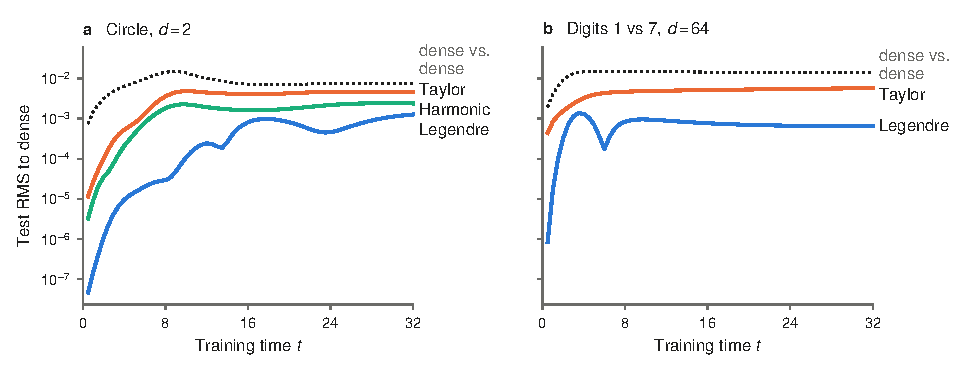
\includegraphics[width=\linewidth]{figures/exp_trajectory.pdf}
\caption{Error to the coupled width-4096 dense reference at every recorded
positive time, mean over three independent coupled references. The dotted
curve is the mean dense-versus-dense discrepancy. Models are those of
\Cref{tab:app-costs}; only declared query inputs are scored.}
\label{fig:app-trajectory}
\end{figure}

\begin{figure}[h]
\centering
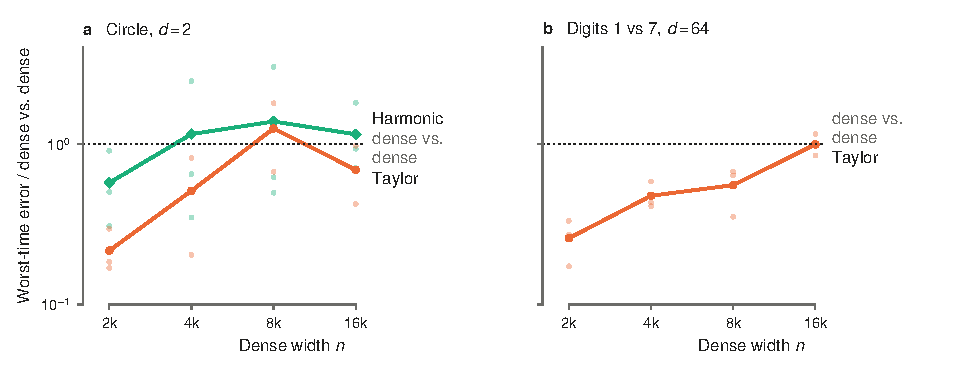
\includegraphics[width=\linewidth]{figures/exp_fixed_budget.pdf}
\caption{A fixed compact width of 512 as the dense reference widens. Each
point is the mean over three pairs of the ratio of the compression's
worst-time error to the dense pair's worst-time error; dots show the
individual pairs. All complete candidates are included, whether or not they
pass. Source settings may vary with dense width.}
\label{fig:app-fixed-budget}
\end{figure}

\begin{figure}[h]
\centering
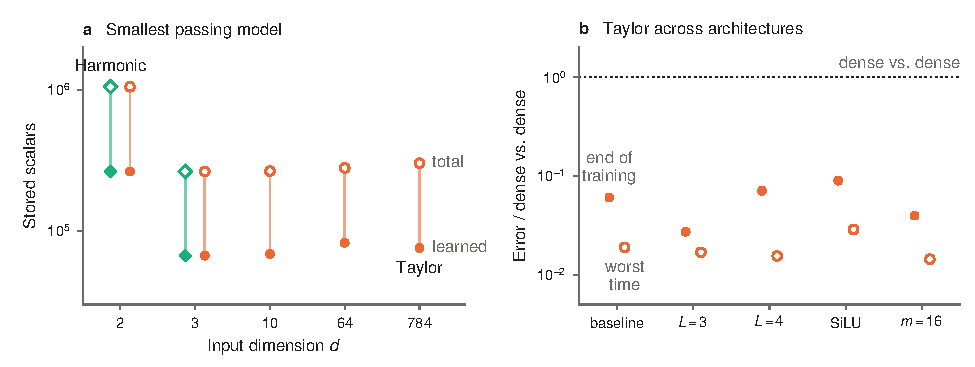
\includegraphics[width=\linewidth]{figures/exp_robustness.pdf}
\caption{(a) Smallest passing learned (filled) and total (hollow) storage
across input dimensions, using the worst-time criterion of
\Cref{fig:exp-storage}; at $d=784$ Taylor uses a fixed, counted projection
onto the panel span. (b) Taylor's endpoint and worst-time errors relative to
dense-versus-dense for five single-seed architecture variants with one
shared configuration: the two-layer baseline, three and four hidden layers,
SiLU activations, and sixteen training inputs.}
\label{fig:app-robustness}
\end{figure}

\begin{figure}[h]
\centering
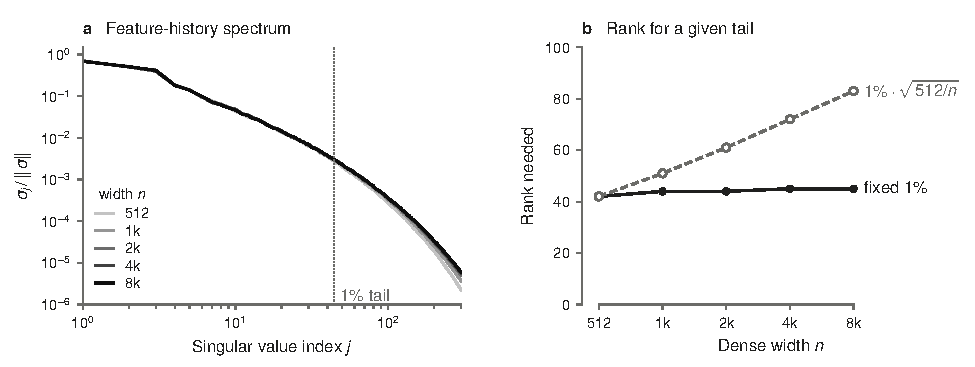
\includegraphics[width=\linewidth]{figures/exp_spectra.pdf}
\caption{(a) Normalized singular values of saved dense feature histories at
five widths. (b) Rank needed to leave a fixed $1\%$ relative tail (solid),
and a tail shrinking like $n^{-1/2}$ (dashed). The mandatory initial span is
additional. Single-seed reconstruction evidence, not a prediction-error
guarantee.}
\label{fig:app-spectra}
\end{figure}

\begin{figure}[h]
\centering
\begin{minipage}[t]{0.49\linewidth}
\centering
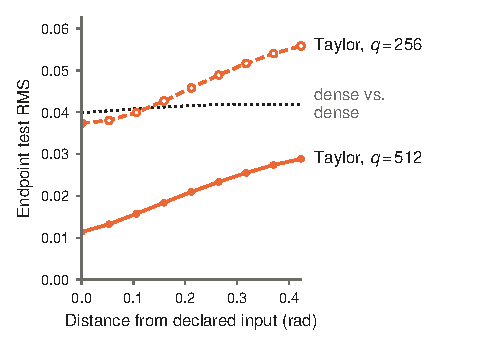
\includegraphics[width=\linewidth]{figures/exp_query_distance.pdf}
\end{minipage}\hfill
\begin{minipage}[t]{0.49\linewidth}
\centering
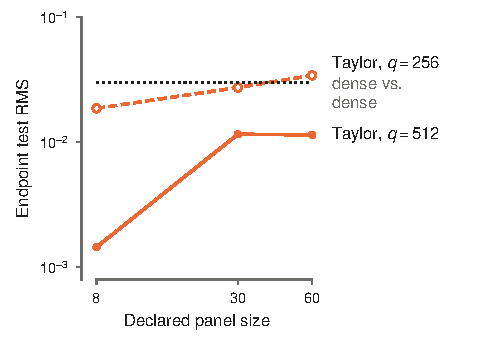
\includegraphics[width=\linewidth]{figures/exp_panel_size.pdf}
\end{minipage}
\caption{Scope of the declared panel. Left: Taylor's endpoint error along six
fixed geodesic paths leaving the declared inputs, for one seed in ambient
dimension 10 with a target depending on three coordinates. Right: panels of
8, 30 and 60 declared inputs at fixed source rank, all scored on the same
original queries. Labels of declared inputs are never used.}
\label{fig:app-panel}
\end{figure}

\begin{figure}[h]
\centering
\begin{minipage}[t]{0.49\linewidth}
\centering
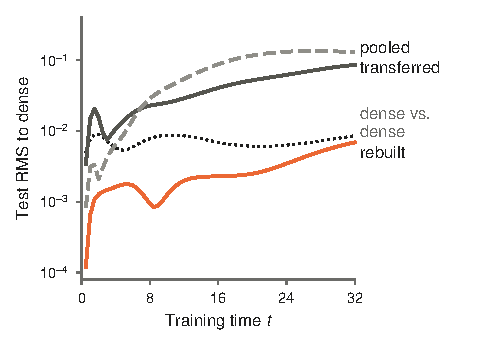
\includegraphics[width=\linewidth]{figures/exp_transfer.pdf}
\end{minipage}
\caption{Changing the labels after the sources are built. Sources rebuilt
for the new labels track the dense reference; sources transferred from the
old labels, or pooled across both, do not. The fixed-data theorem does not
promise label-independent sources.}
\label{fig:app-transfer}
\end{figure}

\begin{figure}[h]
\centering
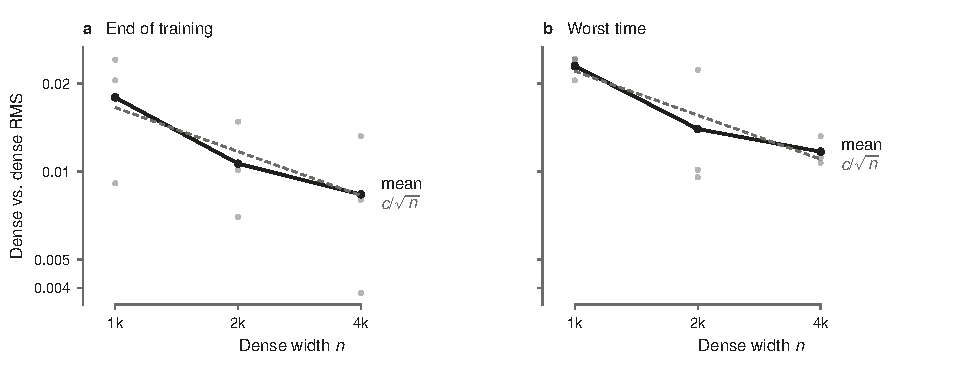
\includegraphics[width=\linewidth]{figures/exp_dense_pairs_sphere.pdf}
\par\medskip
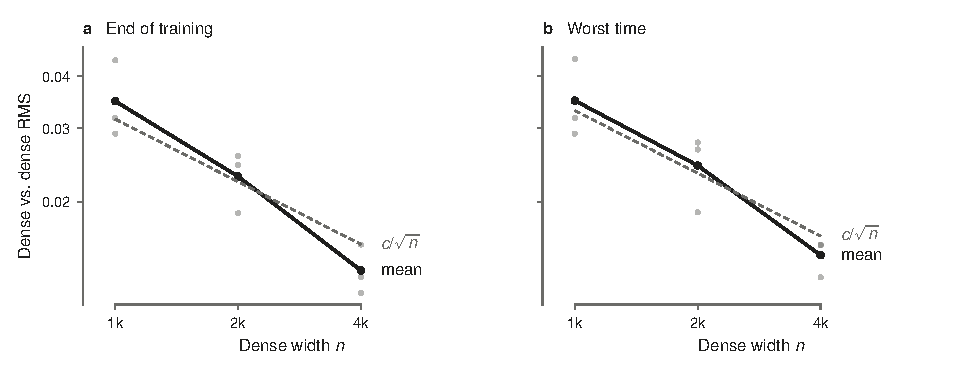
\includegraphics[width=\linewidth]{figures/exp_dense_pairs_mnist.pdf}
\caption{Independent dense discrepancy against width, at the end of
training and at the worst recorded time: sphere with $d=3$ (top) and raw
MNIST 1 versus 7 with $d=784$ (bottom). Three independent pairs per width;
dashed curves are descriptive $c/\sqrt n$ fits.}
\label{fig:app-dense-pairs}
\end{figure}

% Existing static assets only: one PDF per stem, including every gallery page.
% Nonfloating blocks keep each caption with its image and avoid float-only pages.
\clearpage
\section{Figures and numerical illustrations}
\label{cp:figures}
\begingroup
\raggedbottom
\captionsetup{font=small,labelfont=bf,skip=4pt,hypcap=false}
\newcommand{\figureplate}[4][1]{%
  \par\noindent\begin{minipage}{\linewidth}
  \centering
  \includegraphics[page=#1,width=\linewidth,height=#2\textheight,
                   keepaspectratio]{figures/#3.pdf}
  \captionof{figure}{#4}\label{fig:archive:#3:#1}
  \end{minipage}\par\medskip}

This collection preserves the static figures already accompanying the paper,
including alternate layouts and all seven pages of the illustrated gallery.
Format copies and interactive explainers are omitted. These are earlier
illustrations under their recorded protocols, not new experiments or
certificates of the headline theorem. Unless stated otherwise, RMS means
disagreement with dense predictions on sampled queries, not error against
labels. Recorded times do not certify a continuous-time supremum, and
separately fitted endpoints need not share a physical time. Historical
artwork sometimes writes $P$ for the history order $q$. In radial plots,
$f(\theta)$ denotes the prediction at input angle $\theta$.

\figureplate{.23}{mechanism}{Response-memory reconstruction and the
product-of-tails identity. Both histories use the same Legendre modes;
the initialized mixer remains fixed and retained. The printed finite-horizon
rates are schematic, not the present complete-trajectory estimates.}
\figureplate{.32}{memory_mechanism}{Single-sample, three-mode illustration:
paired forward and residual-weighted backward moments reconstruct the learned
connection. The reconstructed network supplies the next responses; the
polynomial basis is fixed while its neuron-valued coefficients evolve.}

\figureplate{.31}{paired_projection}{Projecting both histories onto the same
orthogonal history space cancels the two mixed terms, leaving the pairing of
the omitted histories. Trajectory control additionally requires regularity
and feedback stability.}
\figureplate{.25}{clocks}{Illustrative four-mode fits of a normalized backward
history in physical time and two alternative clocks. The displayed fit errors
describe this example, not a general ordering of clock accuracy.}
\figureplate{.19}{moments}{Three neuron histories reconstructed with one,
two, and three Legendre coefficients, with coefficient distributions below.
Errors are normalized by each history's range. This older nonzero-readout
example illustrates memory coordinates, not the canonical initialization
theorem.}

\figureplate{.39}{learning_clocks}{A constructed smooth response path in
physical time and a clock that also tracks response motion. Matching colors
identify the same events; this is a coordinate-change schematic, not a
measured training trajectory or a constant-speed assertion.}
\figureplate{.39}{learning_in_motion}{Earlier eight-checkpoint circle
comparison: two tanh hidden layers, $n=2048$, and $q=1,3,7$.
Snapshots share physical times; discrepancies use 2048 query angles.
Dotted numerical sensitivities and connecting lines do not certify the
unobserved times.}

\figureplate{.20}{trajectory}{Paired-label circle predictions at common times
$0,5,20,80$: two tanh hidden layers, $n=2048$, $q=1,3,7$.
Radius is $3+f(\theta)$ and black points are training labels.
This is the later 39-checkpoint, two-tolerance Heun replay.}
\figureplate{.28}{trajectory_rms}{Companion dense-versus-memory RMS at the
38 positive common times of that replay. The coarse/fine sensitivity scale
is an empirical numerical diagnostic, not a continuous-time bound.}
\figureplate{.24}{orders}{Deep-circle endpoint discrepancies, coarse/fine
sensitivity, and hidden-feature motion for $q=1,2,3$.
These three-hidden-layer tanh runs have $n=4096$ and individual training-MSE
$10^{-3}$ endpoints; the sensitivity ranges are not confidence intervals.}

\figureplate{.59}{circle_deep}{Five circle tasks with three tanh hidden
layers, $n=4096$, and $q=1,2,3$. Each curve uses its own training-MSE
$10^{-3}$ endpoint: the comparison is between fitted functions, not common
physical times.}
\figureplate{.23}{circles_deep}{Compact radial view of the deep-circle
family. Radius is $3+f(\theta)$; the printed values are RMS differences from
dense predictions on 8192 circle queries. This is an alternate layout,
not an additional experiment.}

\figureplate{.43}{circle_shallow}{Earlier Cartesian circle comparison with
two tanh hidden layers, $n=2048$, and $q=1,3,7$, at individual training-MSE
$10^{-3}$ endpoints. This export uses archived dense references, unlike
the selected references in the radial views.}
\figureplate{.40}{circle_shallow_radial}{Shallow-circle radial comparison at
the same loss threshold. Radius is $3+f(\theta)$; RMS uses 8192 queries
against four fresh dense references and one refined archived reference.
Black points mark training labels.}

\figureplate{.59}{circle_deep_radial}{Larger radial panels for the deep-circle
family: three tanh hidden layers, $n=4096$, $q=1,2,3$, and separately fitted
training-MSE $10^{-3}$ endpoints. The printed discrepancies use 8192 circle
queries; fixed dense mixers remain additional storage.}
\figureplate{.23}{circles_shallow}{Compact radial layout of the shallow-circle
family, using the same selected references as its larger radial view.
The printed RMS values measure fitted-function disagreement, not label risk.}

\figureplate{.39}{order_decay}{Observed circle discrepancy versus history
order in five tasks. The inverse-order reference lines are visual comparisons,
not fitted or certified convergence rates.}

\figureplate{.25}{same_rank}{Selected circle endpoints compare response
memory with two directly trained factor seeds at the same correction-rank
bound. Equal correction rank does not imply equal total storage or a
comparison with every low-rank optimizer.}
\figureplate{.39}{factors}{Paired-label fitted functions and five-task rank
sweeps for two tanh hidden layers of width 2048. RMS uses 8192 queries at
individual training-MSE $10^{-3}$ endpoints; fixed mixers are additional,
and omitted or precision-limited runs are not exact successes.}

\figureplate{.39}{same_rank_dynamics}{Alternate presentation of the factor
comparison, including the rank-24 paired-label example and five-task sweep.
Despite the filename, these are separately fitted endpoints, not common-time
dynamics. Hollow points have limited numerical precision; one capped run is
omitted.}
\figureplate{.39}{same_rank_radial_preview}{Enlarged paired-label comparison:
dense training, order-3 memory, and two factor seeds with correction-rank
bound 24. Radius is $3+f(\theta)$; RMS uses 8192 angles at individual
training-MSE $10^{-3}$ endpoints.}

\figureplate{.39}{frozen_ntk_radial_preview}{Dense training, its full frozen
initial empirical NTK, and order-3 memory from the same width-2048
initialization. Each reaches training MSE $10^{-3}$ at its own time.
Radius is $30+f(\theta)$ here, preserving the large signed NTK excursions.}
\figureplate{.36}{learning_controls_equal_mixed_odd}{Equally spaced
mixed-label control: dense training, frozen initial NTK, two factor seeds,
and order-3 memory. RMS uses 8192 queries at individual training-MSE
$10^{-3}$ endpoints. The correction-rank bound is 12 after the antipodal
quotient.}

\figureplate{.36}{learning_controls_quadrant_alternating}{Quadrant
alternating labels, with the same width-2048 two-hidden-layer tanh control
protocol. The factor correction-rank bound is 24; the NTK panel explicitly
uses a 100-times-wider output scale. RMS is disagreement with dense,
not ground-truth error.}
\figureplate{.36}{learning_controls_quadrant_center_edges}{Quadrant
center-versus-edges labels under the same endpoint protocol. The NTK panel
alone uses a 200-times-wider output scale, with signed ticks in original
units. All reported RMS discrepancies use 8192 circle queries.}

\figureplate{.36}{learning_controls_quadrant_pairs}{Quadrant paired labels:
the same dense, frozen-NTK, rank-24 factor, and order-3 memory comparison.
Each model fits separately to training MSE $10^{-3}$; the NTK output scale
is explicitly widened tenfold.}

\figureplate{.82}{learning_controls_gallery}{Overview of all five preceding
control tasks. This combines the same observations, with marked NTK scale
changes and correction-rank bounds 24 or 12; it is not another replicate.}
\figureplate{.51}{learning_controls_gallery_a}{Page-friendly assembly of
the three quadrant control tasks. The protocols, separate fitted endpoints,
and marked NTK output-scale changes are unchanged.}
\figureplate{.34}{learning_controls_gallery_b}{Companion assembly of the
outlier and equally spaced mixed-label tasks. These are the remaining two
rows of the full control gallery, not additional experiments.}

\figureplate{.27}{mnist}{Earlier MNIST 3-versus-8 comparison: 100 training
and 1984 held-out images, two tanh hidden layers, $n=4096$.
The order-3 agreement plot and order-1--3 differences use individual
training-MSE $10^{-3}$ endpoints. RMS is disagreement with dense predictions.}
\figureplate{.46}{mnist_rms}{MNIST validation discrepancy across history
orders and the displayed training-loss endpoints. Bars show observed
refinement margins, not confidence intervals; open markers identify failures
of the numerical gate.}

\figureplate{.39}{mnist_residuals}{Alternate MNIST endpoint presentation.
Signed memory-minus-dense differences share one vertical scale; order 2 is
slightly closer than order 3 in this run. These are function-agreement
measurements, not classification accuracies.}
\figureplate{.25}{mnist_scatter}{Held-out MNIST predictions for $q=1,2,3$
against dense predictions at the primary training-MSE $10^{-3}$ endpoints.
This scatter layout uses the same endpoint data, not another replicate.}

\figureplate{.41}{sphere_orders}{Sphere illustration with four ReLU hidden
layers, $n=2048$, $m=64$, and 8192 equal-area queries. Both hemispheres and
a shared error scale are shown. Each model stops at training RMS $0.01$;
the single-seed Euler run uses step $1/128$. ReLU is outside the analytic
activation theorem.}
\figureplate{.41}{sphere_comparison}{Dense output, order-3 memory output,
and their signed difference for the same sphere run. Black points are
training locations. This fitted-endpoint illustration has no
continuous-flow refinement certificate.}

\figureplate{.39}{sphere3_time}{Saved sphere-3 query RMS from a width-4096
dense reference over recorded times, with eight training and 30 test inputs.
The export's ``Logarithmic'' family is called Taylor by its adjacent plotting
script, not the seeded decoder below. Dense-control curves aggregate three
small-network seeds and two dense pairs by geometric means.}
\figureplate{.39}{sphere3_tradeoff_endpoint}{Sphere-3 fitted-endpoint RMS
versus moving parameter count. Smaller-dense summaries are medians and
observed ranges over three seeds. ``Logarithmic'' retains the same historical
Taylor-family label; fixed storage and offline setup are additional.}

\figureplate{.39}{sphere3_tradeoff_max_time}{Companion sphere-3 tradeoff for
maximum RMS over recorded times, rather than endpoint RMS. The shaded
small-network range is not a confidence interval; the horizontal axis still
excludes fixed storage and source-construction costs.}
\figureplate{.26}{compression_validation}{Earlier Harmonic circle
confirmation at widths 1024, 2048, and 4096, with three held-out seeds per
width. Curves show maximum-recorded-time query RMS and retained tensor
scalars; shading is the observed seed range. Source setup and query workspace
are additional.}

\figureplate{.26}{compression_logarithmic}{Earlier dimension-five
\emph{seeded decoder}, labelled ``Logarithmic'' in this artwork: finite-program
query fidelity and persistent numerical payload across three widths.
This is not Taylor. The dotted storage curve adds query workspace; flat
payload in these tests is not an asymptotic scaling estimate.}
\figureplate{.23}{compression_checks}{Further Harmonic dimension and
PCA-based digits checks, followed by seeded-decoder dimension checks.
The decoder's circle failure remains visible. Seed counts vary; ranges and
the empirical factor-three threshold are not confidence statements.
The digits task differs from the MNIST100 figures above.}
\figureplate{.26}{learning_controls_two_outliers_alternating}{Remaining
circle control: alternating labels with two outliers, under the earlier
width-2048 tanh endpoint protocol. The NTK output scale is widened tenfold;
RMS measures fitted-function disagreement on 8192 queries.}

\figureplate[1]{.39}{experimental_gallery}{Original illustrated gallery,
page 1: the three-mode memory mechanism. The next six plates preserve the
remaining pages, including their explanatory headings; they reuse earlier
illustrations rather than add experiments.}
\figureplate[2]{.39}{experimental_gallery}{Gallery page 2: the earlier
eight-checkpoint common-time circle comparison, not the later 39-checkpoint
replay. Its numerical sensitivities are diagnostics between saved runs.}
\figureplate[3]{.39}{experimental_gallery}{Gallery page 3: same-correction-rank
factor controls at separately fitted endpoints. Rank equality is not an
equal-total-storage claim.}
\figureplate[4]{.39}{experimental_gallery}{Gallery page 4: the constructed
smooth-path clock illustration. The change of coordinate preserves events,
not necessarily their speed.}
\figureplate[5]{.39}{experimental_gallery}{Gallery page 5: orthogonal pairing
of two histories leaves a product of omitted tails. Feedback stability is a
separate requirement for controlling the evolving network.}
\figureplate[6]{.39}{experimental_gallery}{Gallery page 6: the earlier
MNIST100 fitted-prediction comparison and signed differences. RMS measures
disagreement with dense predictions, not error against labels.}
\figureplate[7]{.39}{experimental_gallery}{Gallery page 7: deep-circle order
sensitivity and hidden-feature motion. Refinement scales are empirical
diagnostics, and the observed order trend need not be monotone.}
\figureplate{.39}{order_sensitivity}{Standalone view of the deep-circle order,
numerical-sensitivity, and feature-motion comparison. Each model uses its own
training-MSE $10^{-3}$ endpoint; order 2 is closer than order 3 on the two
alternating-label tasks, so the observed order trend is not uniformly monotone.}
\endgroup

